\documentclass[11pt]{text/ucsddissertation}
% mathptmx is a Times Roman look-alike (don't use the times package)
% It isn't clear if Times is required. The OGS manual lists several
% "standard fonts" but never says they need to be used.
\usepackage{mathptmx}
\usepackage[NoDate]{currvita}
\usepackage{array}
\usepackage{tabularx}
\usepackage{booktabs}
\usepackage{ragged2e}
\usepackage{microtype}
\usepackage[breaklinks=true,pdfborder={0 0 0}]{hyperref}
\usepackage{graphicx}


\usepackage{text/liquidHaskell}
\usepackage{amsmath,amssymb, latexsym}

\usepackage{amsmath}
\usepackage{amsthm}
\usepackage{thmtools}
\usepackage{text/commands}


\usepackage{stmaryrd}

\usepackage{comment}
\usepackage{flushend}
\usepackage[inference]{semantic}

\usepackage{paralist}

\newtheorem{notation}{Notation}{\itshape}{}
\newtheorem{invariant}{Invariant}
\newtheorem{lemma}{Lemma}
\newtheorem{definition}{Definition}
\newtheorem{lemma*}{Lemma}
\newtheorem{theorem}{Theorem}
\newtheorem{theorem*}{Theorem}
\newtheorem{corollary}{Corollary}
\usepackage{listings}

% uncomment next line to restore colors
% \def\withcolor{}

\ifdefined\withcolor
	\definecolor{haskellblue}{rgb}{0.0, 0.0, 1.0}
	\definecolor{haskellblue}{rgb}{1.0, 0.0, 0.0}
	\definecolor{gray_ulisses}{gray}{0.55}
	\definecolor{castanho_ulisses}{rgb}{0.71,0.33,0.14}
	\definecolor{preto_ulisses}{rgb}{0.41,0.20,0.04}
	\definecolor{green_ulisses}{rgb}{0.0,0.4,0.0}
\else
	\definecolor{haskellblue}{gray}{0.1}
	\definecolor{haskellred}{gray}{0.1}
	\definecolor{gray_ulisses}{gray}{0.1}
	\definecolor{castanho_ulisses}{gray}{0.1}
	\definecolor{preto_ulisses}{gray}{0.1}
	\definecolor{green_ulisses}{gray}{0.1}
\fi


\def\codesize{\normalsize}
\newcommand\showfocus[1]{\color{purple}{\textbf{#1}}}

\lstdefinelanguage{HaskellUlisses} {
	basicstyle=\ttfamily\footnotesize,
	sensitive=true,
	morecomment=[l][\color{gray_ulisses}\ttfamily\codesize]{--},
	%% morecomment=[s][\color{gray_ulisses}\ttfamily\codesize]{\{-}{-\}},
	morestring=[b]",
	moredelim=[is][\showfocus]{\#}{\#},
	stringstyle=\color{haskellred},
	showstringspaces=false,
	numberstyle=\codesize,
	numberblanklines=true,
	showspaces=false,
	breaklines=true,
	showtabs=false,
    literate={
           {dollar}{{$\text{\$}$}}1
           {`}{{{$^{\backprime}{}$}}}1
           {'}{{{$^{\prime}{}$}}}1
           {^label}{{$^{\text{l}}$}}2
           % {QED}{{{\color{lcolor}QED}}}3
           % {***}{{{\color{lcolor}***}}}3
           {?}{{{$\therefore$}}}1
           % {<}{{$<$}}1
           % {>}{{$>$}}1
           {<=}{{$\leq$}}2
           {>>=}{>>=}3
           {>=}{{$\geq$}}2
           {theta}{{$\theta$}}1
           {env}{{$\Gamma$}}1
           {|-}{{$\vdash$}}1
           {<=!}{{{\color{lcolor}<=!}}}3
           {!=}{{$\neq$}}2
           {forall}{{$\forall$}}1
           {->}{{$\rightarrow$}}2
           {=*}{{$\eqfun$}}2
           {<=>}{{$\Leftrightarrow$}}3
           {=>}{{$\Rightarrow$}}2
           {<:}{{$\preceq$}}1
           {mempty}{{$\mempty$}}1
           {mappend}{{$\mappend$}}1
           {<>}{{$\mappend$}}1
           {stringMempty}{{$\stringMempty$}}1
           {<+>}{{$\stringMappend$}}1
           {stringMappend}{{$\stringMappend$}}1
           {listMempty}{{[]}}1
           {listMappend}{{++}}2
           {epsilon}{{$\epsilon$}}1
           {eta}{{$\eta$}}1
           {&&&}{&&&}3
           {&&}{{$\land$}}1
           {_m}{{${}_m$}}1
           {_n}{{${}_n$}}1
           {m^+}{{m${}^{+}$}}2
           {SetMem}{{$\in$}}1
           {Set_cup}{{$\cup$}}1
           {Set_cap}{{$\cap$}}1
           {Set_emp}{{$\emptyset$}}1
           {Set_sub}{{$\subseteq$}}1
           },
	emph=
	{[1]
		FilePath,IOError,abs,acos,acosh,all,and,any,appendFile,approxRational,asTypeOf,asin,
		asinh,atan,atan2,atanh,basicIORun,break,catch,ceiling,chr,compare,concat,concatMap,
		const,cos,cosh,curry,cycle,decodeFloat,denominator,digitToInt,div,divMod,drop,
		dropWhile,either,elem,encodeFloat,enumFrom,enumFromThen,enumFromThenTo,enumFromTo,
		error,even,exp,exponent,fail,filter,flip,floatDigits,floatRadix,floatRange,floor,
		fmap,foldl,foldl1,foldr,foldr1,fromDouble,fromEnum,fromInt,fromInteger,
		fromRational,fst,gcd,getChar,getContents,getLine,head,id,inRange,index,init,intToDigit,
		interact,ioError,isAlpha,isAlphaNum,isAscii,isControl,isDenormalized,isDigit,isHexDigit,
		isIEEE,isInfinite,isLower,isNaN,isNegativeZero,isOctDigit,isPrint,isSpace,isUpper,iterate,
		last,lcm,length,lex,lexDigits,lexLitChar,lines,log,logBase,lookup,map,mapM,mapM_,max,
		maxBound,maximum,maybe,min,minBound,minimum,mod,negate,not,notElem,numerator,odd,
		or,pi,pred,primExitWith,print,product,properFraction,putChar,putStr,putStrLn,quot,
		quotRem,range,rangeSize,read,readDec,readFile,readFloat,readHex,readIO,readInt,readList,readLitChar,
		readLn,readOct,readParen,readSigned,reads,readsPrec,realToFrac,recip,rem,repeat,replicate,
		reverse,round,scaleFloat,scanl,scanl1,scanr,scanr1,seq,sequence,sequence_,show,showChar,showInt,
		showList,showLitChar,showParen,showSigned,showString,shows,showsPrec,significand,signum,sin,
		sinh,snd,span,splitAt,sqrt,subtract,succ,sum,tail,take,takeWhile,tan,tanh,threadToIOResult,toEnum,
		toInt,toInteger,toLower,toRational,toUpper,truncate,uncurry,undefined,unlines,until,unwords,unzip,
		unzip3,userError,words,writeFile,zip,zip3,zipWith,zipWith3,listArray,doParse,for,initTo,
        maxEvens,create,get,set,initialize,idVec,fastFib,fibMemo,
        insert,union,split,size,fromList,initUpto,trim,quickSort,insertSort,append,upperCase,
        copy, group, doDownLoop, mapAccumR, peekByteOff,
        pokeByteOff,spanByte, 
        good, bad, foo, explode, 
        fib, ack, 
        tLen,
        memcpy,writeChar,unsafeWrite,unsafeFreeze,
        singleton
	},
	emphstyle={[1]\color{haskellblue}},
	emph=
	{[2]
		Bool,Char,Double,Either,Float,IO,Integer,Int,Maybe,Ordering,Rational,Ratio,ReadS,ShowS,String,
		Word8,Nat,NonZero,Nat64,Text,ByteString,ByteStringSZ,ByteStringN,
        Ptr,ForeignPtr,CSize
        InPacket,Tree,Prop,TreeEq,TreeLt,Vec,
        NullTerm,IncrList,DecrList,UniqList,BST,MinHeap,MaxHeap,
        PtrN,ByteStringN,ByteStringEq,VO,ByteStringsEq,ByteStringNE
	},
	emphstyle={[2]\color{castanho_ulisses}},
	emph=
	{[3]
		case,class,data,deriving,do,else,if,return,def,import,in,infixl,infixr,instance,let,
		module,measure,predicate,of,primitive,then,refinement,type,where,lazy, type, bound
	},
	emphstyle={[3]\color{preto_ulisses}\textbf},
	emph=
	{[4]
		quot,rem,div,mod,elem,notElem,seq
	},
	emphstyle={[4]\color{castanho_ulisses}\textbf},
	emph=
	{[5]
		PS,Tip,Node,EQ,False,GT,Just,LT,Left,Nothing,Right,True,Show,Eq,Ord,Num
	},
	emphstyle={[5]\color{green_ulisses}}
}

%%%ORIG
%%%\lstnewenvironment{code}
%%%{\textbf{Haskell Code} \hspace{1cm} \hrulefill \lstset{language=HaskellUlisses}}
%%%{\hrule\smallskip}

%V1
%\lstnewenvironment{code}
%{\smallskip \lstset{language=HaskellUlisses}}
%{\smallskip}

\lstnewenvironment{code}
{\lstset{language=HaskellUlisses}}
{}

\lstnewenvironment{mcode}
{\lstset{language=HaskellUlisses,columns=fullflexible,keepspaces,mathescape}}
{}


\lstMakeShortInline[language=HaskellUlisses,mathescape,keepspaces,mathescape,basicstyle=\ttfamily\normalsize,breakatwhitespace]@


%\lstMakeShortInline[language=HaskellUlisses,basicstyle=\ttfamily\normalsize,breakatwhitespace]@



\AtBeginDocument{%
	\settowidth\cvlabelwidth{\cvlabelfont 0000--0000}%
}

% OGS recommends increasing the margins slightly.
\increasemargins{.1in}

% These are just for testing/examples, delete them
\usepackage{trace}
%\usepackage{showframe} % This package was just to see page margins
\usepackage[english]{babel}
\usepackage{blindtext}
\overfullrule5pt
% ---

% Required information
\title{Liquid Haskell: Haskell as a Theorem Prover}
\author{Niki Vazou}
\degree{Computer Science}{Doctor of Philosophy}
% Each member of the committee should be listed as Professor Foo Bar.
% If Professor is not the correct title for one, then titles should be
% omitted entirely.
\chair{Professor Ranjit Jhala}
% Your committee members (other than the chairs) must be in alphabetical order
\committee{Professor Samuel R. Buss}
\committee{Professor Cormac Flanagan}
\committee{Professor Sorin Lerner}
\committee{Professor Daniele Micciancio}
\degreeyear{2016}

% Start the document
\begin{document}

\chapter{Related Work}\label{chapter:related}

\section{Refinement Types in Practice}\label{sec:realword:related}

Next, we situate \toolname with 
existing Haskell verifiers.

\spara{Dependent Types} are the basis of many verifiers, 
or more generally, proof assistants.
%
Verification of haskell code is possible with
``full'' dependently typed systems like Coq~\cite{coq-book}, 
Agda~\cite{norell07}, Idris~\cite{Brady13}, Omega~\cite{Sheard06}, and
 {$\lambda_\rightarrow$}~\cite{LohMS10}.
 %
 While these systems are highly expressive,
their expressiveness comes at the cost of making logical validity checking undecidable
thus rendering verification cumbersome.	
 %
 Haskell itself can be considered a dependently-typed language,
 as type level computation is allowed via 
 Type Families~\cite{McBride02},
 Singleton Types\cite{Weirich12}, 
 Generalized Algebraic  Datatypes (GADTs)~\cite{JonesVWW06, SchrijversJSV09}, 
 and type-level functions~\cite{ChakravartyKJ05}.
 %
Again, 
verification in haskell itself turns out to be quite painful~\cite{LindleyM13}.

\spara{Refinement Types} are a form of dependent types where 
invariants are encoded via a combination of types and predicates
from a restricted \emph{SMT-decidable} 
logic~\cite{Rushby98,pfenningxi98,Dunfield07,GordonTOPLAS2011}. 
%
\toolname uses Liquid Types~\cite{LiquidPLDI09} 
that restrict the invariants even more
to allow type inference, a crucial feature of a usable type system.
%
Even though the language of refinements is restricted,
as we presented, the combination of
Abstract Refinements~\cite{vazou13} 
with sophisticated measure definitions 
allows specification and verification of a wide variety 
of program properties.

\spara{Static Contract Checkers} 
like ESCJava~\cite{ESCJava} are a classical way of verifying 
correctness through assertions and pre- and post-conditions. 
%
\cite{XuPOPL09} describes a static contract checker for 
Haskell that uses symbolic execution to unroll procedures
upto some fixed depth, yielding weaker ``bounded'' soundness
guarantees.
% 

Similarly, Zeno~\cite{ZENO} is an automatic Haskell 
prover that combines unrolling with heuristics for rewriting
and proof-search. 
%%Based on rewriting, it is sound but 
%%``Zeno might loop forever'' when faced with 
%%non-termination.
%
Finally, the Halo~\cite{halo} contract checker encodes 
Haskell programs into first-order logic by directly 
modeling the code's denotational semantics,
again, requiring heuristics for instantiating axioms 
describing functions' behavior.
%


\spara{Totality Checking}
is feasible by GHC itself, via an option flag that warns of any incomplete patterns.
%
Regrettably, GHC's warnings are local, \ie
GHC will raise a warning for @head@'s partial definition, 
but not for its caller, as the programmer would desire.
%%(2)~ and preservative:
%%a warning will be raised for any incomplete pattern
%%without an attempt to reason if it is reachable or not.
%
Catch~\cite{catch}, 
a fully automated tool that tracks incomplete patterns,
addresses the above issue
%
by computing functions' pre- and post-conditions.
Moreover, catch statically analyses the code 
to track reachable incomplete patterns.
%
\toolname allows more precise analysis than catch, 
thus, by assigning the appropriate
types to $\star$Error functions (\S~\ref{sec:totality}) 
it tracks reachable incomplete patters 
%we get catch analysis
as a side-effect of verification.

\spara{Termination Analysis}
is crucial for \toolname's soundness 
and is implemented in a technique inspired by~\cite{XiTerminationLICS01}, 
%
Various other authors have proposed techniques to verify termination of
recursive functions, either using the ``size-change
principle''~\cite{JonesB04,Sereni05}, or by annotating types with size indices
and verifying that the arguments of recursive calls have smaller
indices~\cite{HughesParetoSabry96,BartheTermination}.
%
To our knowledge, none of the above analyses have been empirically
evaluated on large and complex real-world libraries.

AProVE~\cite{Giesl11} implements a powerful, fully-automatic
termination analysis for Haskell based on term-rewriting.
%
Compared to AProVE,
encoding the termination proof via 
refinements provides advantages that are crucial in 
large, real-world code bases. 
Specifically, refinements
let us
%
(1) prove termination over a subset 
    (not all) of inputs; many functions (\eg @fac@) 
    terminate only on @Nat@ inputs and not all @Int@s,
%
(2) encode pre-conditions, 
    post-conditions, and auxiliary invariants that 
    are essential for proving termination, (\eg @qsort@),
%
(3) easily specify non-standard 
    decreasing metrics and prove termination, (\eg @range@).
%
In each case, the code could be (significantly) 
\emph{rewritten} to be amenable to AProVE but this defeats
the purpose of an automatic checker.
%


\section{Refinement Types for Haskell}\label{sec:refinedhaskell:related}

Next we situate our work with closely related lines of research.

\spara{Dependent Types} are the basis of many verifiers, 
or more generally, proof assistants.
%
In this setting arbitrary terms may appear inside types,
so to prevent logical inconsistencies, and enable
the checking of type equivalence, all terms must
terminate.
%
``Full'' dependently typed systems like Coq~\cite{coq-book}, 
Agda~\cite{norell07}, and Idris~\cite{Brady13} typically use 
\emph{structural} checks where recursion is allowed on 
sub-terms of ADTs to ensure that \emph{all} terms terminate.
%
We differ in that, since the refinement logic is
restricted, we do not require that all functions terminate,
and hence, we can prove properties of possibly diverging 
functions like @collatz@ as well as lazy functions like @repeat@.
%
Recent languages like Aura~\citep{AURA} and Zombie~\citep{Zombie}
allow general recursion, but constrain the logic to a terminating 
sublanguage, as we do, to avoid reasoning 
about divergence in the logic.
%
In contrast to us, the above systems crucially assume 
\emph{call-by-value} semantics to ensure that binders are bound
to values, \ie cannot diverge.





   Haskell itself can be used to \emph{fake} ``lightweight'' dependent 
   types~\citep{ChakravartyKJ05,JonesVWW06,Weirich12}.
   In this style, the invariants are expressed in 
   a restricted~\citep{Jia10} total 
   index language and relationships (\eg $x<y$ and $y<z$) 
   are combined (\eg $x<z$) by explicitly constructing
   a term denoting the consequent from terms 
   denoting the antecedents.
   %
   On the plus side this ``constructive'' approach
   ensures soundness. 
   It is impossible to witness inconsistencies, 
   as doing so triggers diverging computations.
   %
   However, it is not easy to use restricted indices
   with explicitly constructed relations to verify 
   complex properties~\citep{hasochism}.


\spara{Refinement Types} are a form of dependent types where 
invariants are encoded via a combination of types and predicates
from a restricted \emph{SMT-decidable} 
logic~\cite{Rushby98,pfenningxi98,Dunfield07,GordonTOPLAS2011}. 
%
The restriction makes it safe to support arbitrary recursion, 
which has hitherto never been a problem for refinement types.
%
However, we show that this is because all the above systems 
implicitly assume that all free variables are bound to values, 
which is only guaranteed under CBV and, as we have seen, leads 
to unsoundness under lazy evaluation.



\spara{Tracking Divergent Computations}
The notion of type stratification to track potentially 
diverging computations dates to at least~\citep{ConstableS87} 
which uses $\bar{\typ}$ to encode diverging terms, and types 
$\efix{}$ as $(\bar{\typ}\rightarrow\bar{\typ}) \rightarrow \bar{\typ}$).
%
More recently, \cite{Capretta05} tracks diverging 
computations within a \emph{partiality monad}.
%
Unlike the above, we use refinements to 
obtain terminating fixpoints (\etfix{}), which let us prove 
the vast majority (of sub-expressions) in real world libraries 
as non-diverging, avoiding the restructuring that would
be required by the partiality monad.

\spara{Termination Analyses}
Various authors have proposed techniques to verify termination 
of recursive functions, either using the ``size-change principle'' 
\cite{JonesB04,Sereni05}, or by annotating types with size indices 
and verifying that the arguments of recursive calls have smaller 
indices~\cite{HughesParetoSabry96,BartheTermination}.
%
Our use of refinements to encode terminating fixpoints is most 
closely related to~\cite{XiTerminationLICS01}, but this work 
also crucially assumes CBV semantics for soundness.

AProVE~\cite{Giesl11} implements a powerful, fully-automatic
termination analysis for Haskell based on term-rewriting.
%
While we could use an external analysis like AProVE,
we have found that encoding the termination proof via 
refinements provided advantages that are crucial in 
large, real-world code bases. Specifically, refinements
let us
%
(1) prove termination over a subset 
    (not all) of inputs; many functions (\eg @fac@) 
    terminate only on @Nat@ inputs and not all @Int@s,
%
(2) encode pre-conditions, 
    post-conditions, and auxiliary invariants that 
    are essential for proving termination, (\eg @gcd@),
%
(3) easily specify non-standard 
    decreasing metrics and prove termination, (\eg @range@).
%
In each case, the code could be (significantly) 
\emph{rewritten} to be amenable to AProVE but this defeats
the purpose of an automatic checker.
%
Finally, none of the above analyses have been empirically
evaluated on large and complex real-world libraries.


\spara{Static Contract Checkers} 
like ESCJava~\cite{ESCJava} are a classical way of verifying 
correctness through assertions and pre- and post-conditions. 
%
Side-effects like modifications of global variables are a 
well known issue for static checkers for imperative languages;
the standard approach is to use an effect analysis to determine
the ``modifies clause'' \ie the set of globals modified by a procedure.
%
Similarly, one can view our approach as implicitly computing 
the non-termination effects.
%
%
\cite{XuPOPL09} describes a static contract checker for 
Haskell that uses symbolic execution to unroll procedures
upto some fixed depth, yielding weaker ``bounded'' soundness
guarantees.
% 

%
Similarly, Zeno~\cite{ZENO} is an automatic Haskell 
prover that combines unrolling with heuristics for rewriting
and proof-search. 
Based on rewriting, it is sound but 
``Zeno might loop forever'' when faced with 
non-termination.
%
Finally, the Halo~\cite{halo} contract checker encodes 
Haskell programs into first-order logic by directly 
modeling the code's denotational semantics,
again, requiring heuristics for instantiating axioms 
describing functions' behavior. Halo's translation of Haskell
programs directly encodes constructors as uninterpreted functions,
axiomatized to be injective (as the denotational semantics requires).
This heavyweight encoding is more precise than predicate abstraction 
but leads to model-theoretic problems (outlined in the Halo paper) and 
affects the efficiency of the encoding when scaling to larger programs 
(see also \ref{sec:refinedhaskell:conclusion}, paragraph B) in the lack of specialized 
decisions procedures.
%
Unlike any of the above, our type-based approach does 
not rely on heuristics for unrolling recursive procedures, 
or instantiating axioms. 
%
Instead we are based on decidable SMT validity 
checking and abstract interpretation~\cite{LiquidPLDI08} 
which makes the tool predictable and the overall workflow
scale to the verification of large, real-world
code bases.

\section{Abstract Refinement Types}\label{sec:related}

The notion of type refinements was introduced by Freeman and
Pfenning~\cite{FreemanPfenning91}, with refinements limited to
restrictions on the structure of algebraic datatypes, for which
inference is decidable.
%
Our present notion of refinement types has its roots in the
\emph{indexed types} of Xi and Pfenning~\cite{pfenningxi98}, wherein
data types' ranges are restricted by \emph{indices}, analogous to our
refinement predicates, drawn from a decidable domain; in the example
case explored by Xi and Pfenning, types were indexed by terms from
Presburger arithmetic.
%
Since then, several approaches to developing richer refinement type
systems and accompanying methods for type checking have been
developed.
%
Knowles and Flanagan~\cite{Knowles10} allow refinement predicates to
be arbitrary terms of the language being typechecked and present a
technique for deciding some typing obligations statically and
deferring others to runtime.
%; Gronksi \etal~\cite{Gronski06} present animplementation of such a system.
%
Findler and Felleisen's~\cite{Findler02} higher-order contracts, which
extend Eiffel's~\cite{MeyerBook} first-order contracts --- ordinary
program predicates acting as dynamic pre- and post-conditions --- to
the setting of higher-order programs, eschew any form of static
checking, and can be seen as a dynamically-checked refinement type
system.
%
Bengtson \etal~\cite{GordonTOPLAS2011} present a refinement type
system in which type refinements are drawn from a decidable logic,
making static type checking tractable.
%
Greenberg \etal~\cite{Greenberg11} gives a rigorous treatment of the
metatheoretic properties of such a refinement type system.

Refinement types have been applied to the verification of a variety of
program properties~\cite{pfenningxi98,Dunfield,GordonTOPLAS2011,FournetCCS11}.
%
In the most closely related work to our own, Kawaguchi \etal~\cite{LiquidPLDI09} 
introduce \emph{recursive} and \emph{polymorphic} refinements for data
structure properties.
%
The present work unifies and generalizes these two somewhat ad-hoc notions 
into a single, strictly and significantly more expressive mechanism of
abstract refinements.

%  Higher-order logics: Coq/HTT/F*/Agda which have explicit predicates, quantification 
A number of higher-order logics and corresponding verification tools
have been developed for reasoning about programs.
%
Example of systems of this type include NuPRL \cite{Constable86},
%F$_{<:}$ \cite{Cardelli91},
Coq \cite{coq-book}, F$^\star$ \cite{SwamyCFSBY11} and Agda \cite{norell07}
which support the development and verification of higher-order, 
pure functional programs.
%
While these systems are highly expressive, their expressiveness comes at the
cost of making logical validity checking undecidable.
%
To help automate validity checking, both built-in and user-provided
tactics are used to attempt to discharge proof obligations; however,
the user is ultimately responsible for manually proving any
obligations which the tactics are unable to discharge.

\section{Bounded Refinement Types}\label{sec:abstractrefinements:related}

\paragraph{Higher order Logics and Dependent Type Systems}
%
including
NuPRL~\citep{Constable86},
Coq~\citep{coq-book}, Agda~\citep{norell07},
and even to some extent, \haskell~\citep{JonesVWW06, McBride02},
occupy the maximal extreme of the expressiveness spectrum.
However, in these settings, checking requires explicit
proof terms which can add considerable programmer overhead.
%
Our goal is to eliminate the programmer overhead of
proof construction by restricting specifications to
decidable, first order logics and to see how far
we can go without giving up on expressiveness.
%
The \fstar system enables full dependent typing via
SMT solvers via a higher-order universally quantified
logic that permit specifications similar to ours
(\eg @compose@, @filter@ and @foldr@).
%% https://github.com/FStarLang/FStar/
%
While this approach is at least as expressive
as bounded refinements it has two drawbacks.
%
First, due to the quantifiers, the generated VCs
fall outside the SMT decidable theories.
This renders the type system undecidable (in theory),
forcing a dependency on the solver's unpredictable
quantifier instantiation heuristics (in practice).
%
Second, more importantly, % perhaps more importantly,
the higher order
predicates must be \emph{explicitly} instantiated,
placing a heavy annotation burden on the programmer.
%
In contrast, bounds permit decidable
checking, and are automatically instantiated
via Liquid Types.


\paragraph{Our notion of Refinement Types}
%
has its roots in the predicate subtyping
of PVS~\cite{Rushby98} and \emph{indexed types}
(DML~\cite{pfenningxi98}) where types are constrained
by predicates drawn from a logic.
%
To ensure decidable checking several refinement
type systems including~\citep{pfenningxi98,Dunfield07,LiquidICFP14}
restrict refinements to decidable, quantifier free logics.
%
While this ensures predictable checking and inference~\cite{LiquidPLDI08}
it severely limits the language of specifications, and makes it hard to
fashion simple higher order abstractions like @filter@ (let alone the more
complex ones like relational algebras and state transformers.)

\paragraph{To Reconcile Expressiveness and Decidability}
%
\catalyst~\citep{catalyst} permits a form of
higher order specifications where refinements
are relations which may themselves be parameterized
by other relations, which allows for example, a
way to precisely type @filter@ by suitably
composing relations.
%
However, to ensure decidable checking, \catalyst
is limited to relations that can be specified as
catamorphisms over inductive types, precluding
for example, theories like arithmetic.
More importantly, (like \fstar), \catalyst provides
no inference: higher order relations must be
\emph{explicitly} instantiated.
%
Bounded refinements build directly upon
abstract refinements~\citep{vazou13},
a form of refinement polymorphism
analogous to parametric polymorphism.
%
While \cite{vazou13} adds expressiveness via
abstract refinements, without bounds we cannot
specify any \emph{relationships between} the
abstract refinements. The addition of bounds
makes it possible to specify and verify the examples
shown in this paper,
while preserving decidability and inference.

\paragraph{Our Relational Algebra Library} builds on a long
line of work on type safe database access.
%
The HaskellDB~\citep{haskellDB}
showed how phantom types could be used to eliminate
certain classes of errors.
%
Haskell's HList library~\citep{heterogeneous}
extends this work with type-level computation
features to encode heterogeneous lists, which
can be used to encode database schema, and
(unlike HaskellDB) statically reject accesses
of ``missing'' fields.
%
The HList implementation is non-trivial,
requiring new type-classes for new operations
(\eg @append@ing lists); \citep{thepipower}
shows how a dependently typed language greatly
simplifies the implementation.
%
Much of this simplicity can be recovered in
Haskell using the @singleton@ library~\citep{Weirich12}.
%
Our goal is to show that bounded refinements
are expressive enough to permit the construction
of rich abstractions like a relational algebra
and generic combinators for safe database access
while using SMT solvers to provide decidable
checking and inference. Further, unlike the
HList based approaches, refinements they can
be used to \emph{retroactively} or \emph{gradually}
verify safety; if we erase the types we still
get a valid Haskell program operating over
homogeneous lists.


\paragraph{Our Approach for Verifying Stateful Computations} using monads
indexed by pre- and post-conditions is inspired by the method of
Filli\^atre~\citep{Filliatre98}, which was later enriched with
separation logic in Ynot~\citep{ynot}. In future work it would
be interesting to use separation logic based refinements to specify
and verify the complex sharing and aliasing patterns allowed by Ynot.
%
\fstar encodes stateful computations in a special Dijkstra
Monad~\citep{dijkstramonad} that replaces the two assertions with
a single (weakest-precondition) predicate transformer which
can be composed across sub-computations to yield a transformer
for the entire computation.
%
Our \RIO approach uses the idea of indexed monads but
has two concrete advantages.
%
First, we show how bounded refinements alone suffice to
let us fashion the \RIO abstraction from scratch.
%
Consequently, second, we automate inference of pre- and
post-conditions and loop invariants as refinement instantiation
via Liquid Typing~\citep{LiquidPLDI08}.


\section{Refinement Reflection}\label{sec:refinementreflection:related}

% We compare refinement reflection to the most closely related
% lines of work in the vast literature on program verification.

\mypara{SMT-Based Verification}
%
SMT-solvers have been extensively used to automate
program verification via Floyd-Hoare logics~\cite{Nelson81}.
%
Our work is inspired by Dafny's Verified
Calculations~\citep{LeinoPolikarpova16},
a framework for proving theorems in
Dafny~\citep{dafny}, but differs in
%
(1)~our use of reflection instead of axiomatization and
(2)~our use of refinements to compose proofs.
%
Dafny, and the related \fstar~\citep{fstar}
which like \toolname, uses types to compose
proofs, offer more automation by translating
recursive functions to SMT axioms.
However, unlike reflection, this axiomatic
approach renders typechecking and verification
undecidable (in theory) and leads to
unpredictability and divergence
(in practice)~\citep{Leino16}.
%\NV{CHECL Relational-F*, Barthe et al, from POPL 2014, and EasyCrypt}

%% In a work more closely related to
%% ours, \fstar uses refinement types
%% for program verification supporting
%% expressiveness of fully dependent types.
%% %
%% As in Dafny, \fstar directly translates
%% recursive functions to axioms in the logic
%% thus suffers from the ``butterfly effect''
%% and allows the user to explicitly write SMT tactics to control it.

%% Leino \etal~\citep{Leino16}
%% name this problem as the ``butterfly
%% effect'', in which minor modifications
%% to the program source cause significant
%% instabilities in verification and propose
%% trigger selection strategies to address it.
%% %
%% We avoid the ``butterfly effect'' by not
%% directly axiomatizing functions into logic.
%% Instead the information about the function's
%% body is exactly captured in function's result
%% type and user needs to explicitly invoke the function to push
%% the function's definition information into the logic.


\mypara{Dependent types}
%
Our work is also inspired by dependently typed
systems like Coq~\citep{coq-book} and
Agda~\citep{agda}.
%
Reflection shows how deep specification
and verification in the style of Coq and Agda
can be \emph{retrofitted} into existing languages
via refinement typing.
%
Furthermore, we can use SMT to significantly
automate reasoning over important theories like
arithmetic, equality and functions.
%
It would be interesting to investigate how
the tactics and sophisticated proof search
of Coq \etc can be adapted to the refinement setting.

% which allow for arbitrary expressiveness of the type system
% in the cost of automatic verification.
%
%% The syntax of \libname's operators is inspired by
%% Equational Reasoning in Agda~\citep{agda}.
%% Here we extended these equational operators
%% to support linear arithmetic and, for example, prove
%% properties of Ackermann function.
%% %
%% Unlike Adga, proof term are explicit in \libname,
%% we do not use heuristics to infer proofs.


\mypara{Dependent Types for Non-Terminating Programs}
%
Zombie~\citep{Zombie, Sjoberg2015} integrates
dependent types in non terminating programs
and supports automatic reasoning for equality.
%
Vazou \etal have previously~\citep{Vazou14} shown
how Liquid Types can be used to check
non-terminating programs.
%
Reflection makes \toolname at least as
expressive as Zombie, \emph{without}
having to axiomatize the theory of
equality within the type system.
%
Consequently, in contrast to Zombie,
SMT based reflection lets \toolname
verify higher-order specifications
like @foldr_fusion@.

% which lets us use SMT automation
% to verify deep specifications of
% non-trivial programs.
%
% Our current extension is orthogonal to the
% previous work: our system remains sound as
% long as logical terms provably terminate.
%
% We get automation from SMT solvers for not only
% the theory of equality, but also linear arithmetic.
%
% \NV{Zombie with rewritting does not allow HIGHER ORDER reasoning}

\mypara{Dependent Types in Haskell}
%
Integration of dependent types into Haskell
has been a long standing goal that dates back
to Cayenne~\citep{cayenne}, a Haskell-like,
fully dependent type language with undecidable
type checking.
%
In a recent line of work~\citep{EisenbergS14}
Eisenberg \etal aim to allow fully dependent
programming within Haskell, by making
``type-level programming ... at least as
  expressive as term-level programming''.
%
Our approach differs in two significant ways.
%
First, reflection allows SMT-aided verification,
which drastically simplifies proofs over key theories
like linear arithmetic and equality.
%
Second, refinements are completely erased at run-time.
That is, while both systems automatically lift Haskell
code to either uninterpreted logical functions
or type families, with refinements, the logical
functions are not accessible at run-time and
promotion cannot affect the semantics of
the program.
%
As an advantage (resp. disadvantage), refinements
cannot degrade (resp. optimize)
the performance of programs.

\mypara{Proving Equational Properties}
% of Haskell Programs}
%
Several authors have proposed tools for proving
(equational) properties of (functional) programs.
%
Systems~\citep{sousa16} and \citep{KobayashiRelational15}
extend classical safety verification algorithms,
respectively based on Floyd-Hoare logic and Refinement Types,
to the setting of relational or $k$-safety properties
that are assertions over $k$-traces of a program.
%
Thus, these methods can automatically prove that
certain functions are associative, commutative \etc.
but are restricted to first-order properties and
are not programmer-extensible.
%
Zeno~\citep{ZENO} generates proofs by term
rewriting and Halo~\citep{halo} uses an axiomatic
encoding to verify contracts.
%
Both the above are automatic, but unpredictable and not
programmer-extensible, hence, have been limited to
far simpler properties than the ones checked here.
%
HERMIT~\citep{Farmer15} proves equalities by rewriting
the GHC core language, guided by user specified scripts.
%
In contrast, our proofs are simply Haskell programs,
we can use SMT solvers to automate reasoning, and,
most importantly, we can connect the validity of
proofs with the semantics of the programs.

% \RJ{say: hermit does typeclass laws}
%
% \NV{TO ADD Naoki and class laws for TFP}
%
%% Compared to these systems, our proofs are
%% expressed as Haskell programs and do not
%% require the user to learn a different
%% tactic languages.
%% %
%% Moreover, our system is more general
%% as it allows for both equational
%% and linear arithmetic proofs.
%% %
%% On the other hand, \libname requires
%% explicit proofs and does not currently
%% support any automatic heuristics.

\mypara{Deterministic Parallelism}
%
Deterministic parallelism has plenty of theory but relatively few practical
implementations.  Early discoveries were based on limited producer-consumer
communication, such as single-assignment variables \cite{Tesler-1968,IStructures}, Kahn
process networks~\cite{kahn-1974}, and synchronous dataflow~\cite{lee-sdf}.
Other models use synchronous updates to shared state, as in
Esterel~\cite{synchronous-overview} or PRAM.  Finally, work on type systems for
permissions management \cite{permission-types,habanero-java-permissions},
supports the development of {\em non-interfering} parallel programs that access
disjoint subsets of the heap in parallel.  Parallel functional programming is
also non-interfering~\cite{manticore,multicore-ghc}.
%
Irrespective of which theory is used to support deterministic parallel
programming, practical implementations such as Cilk~\cite{cilk} or Intel
CnC~\cite{cnc} are limited by host languages with type systems insufficient to
limit side effects, much less prove associativity.  Conversely, dependently
typed languages like Agda and Idris do not have parallel programming APIs and
runtime systems.

% synchronous languages such as Esterel


\section{String Matcher}\label{sec:stringmatcher:related}


\paragraph{SMT-Based Verification}
%
SMT solvers have been extensively used to automate
reasoning on verification languages like
Dafny~\cite{dafny}, Fstar~\cite{fstar} and Why3~\cite{why3}.
%
These languages are designed for verification,
thus have limited support for commonly used language
features like parallelism and optimized libraries
that we use in our verified implementation.
%
Refinement Types~\cite{ConstableS87,FreemanPfenningDONTCITE91,Rushby98}
on the other hand, target existing general purpose languages,
such as
ML~\cite{pfenningxi98,GordonRefinement09,LiquidPLDI08},
C~\cite{deputy,LiquidPOPL10},
Haskell~\cite{Vazou14},
Racket~\cite{RefinedRacket}
and Scala~\cite{refinedscala}.
However, before Refinement Reflection~\cite{reflection} was introduced,
they only allowed ``shallow'' program specifications,
that is, properties that only talk about behaviors of program functions
but not functions themselves.
%

\paragraph{Dependent Types}
Unlike Refinement Types, dependent type systems,
like Coq~\cite{coq-book}, Adga~\cite{agda} and Isabelle/HOL~\cite{isabelle} allow for ``deep'' specifications
which talk about program functions,
such as the program equivalence reasoning we presented.
%
Compared to (Liquid) Haskell,
these systems allow for tactics and heuristics
that automate proof term generation
but lack SMT automations and
general-purpose language features,
like non-termination, exceptions and IO.
%
Zombie~\cite{Zombie,Sjoberg2015} and Fstar~\cite{fstar} allow dependent types to
coexist with divergent and effectful programs,
but still lack the optimized libraries,
like @ByteSting@, which come
with a general purpose language
with long history, like Haskell.



\paragraph{Parallel Code Verification}
Dependent type theorem provers have been used before to
verify parallel code.
%
BSP-Why~\cite{bspwhy} is an extension to Why2 that is using both Coq and SMTs
to discharge user specified verification conditions.
%
Daum~\cite{daum07} used Isabelle to formalize the semantics
of a type-safe subset of C, 
by extending Schirmer's~\cite{schirmer06}
formalization of sequential imperative languages.
%
Finally, Swierstra~\cite{wouter10} formalized mutable arrays in Agda
and used them to reason about distributed maps and sums.

One work  closely related to ours is
SyDPaCC~\cite{SyDPaCC}, a Coq library that
automatically parallelizes list homomorphisms
by extracting parallel Ocaml versions of user provided Coq functions.
%
Unlike SyDPaCC, we are not automatically generating the parallel
function version, because of engineering limitations
(\S~\ref{sec:evaluation}).  Once these are addressed, code extraction
can be naturally implemented by turning
Theorem~\ref{theorem:two-level} into a Haskell type class with a
default parallelization method.
%
SyDPaCC used maximum prefix sum as a case study,
whose morphism verification is
much simpler than our string matching case study.
%
Finally, our implementation consists of
2K lines of Liquid Haskell, which we consider verbose and aim to
use tactics to simplify.
On the contrary, the SyDPaCC implementation
requires three different languages:
2K lines of Coq with tactics, 600 lines of Ocaml and 120 lines of C,
and is considered ``very concise''.





\begin{comment}
% Begin with frontmatter and so forth
\frontmatter
\maketitle
\makecopyright
\makesignature
% Optional
\begin{dedication}
\setsinglespacing
\raggedright % It would be better to use \RaggedRight from ragged2e
\parindent0pt\parskip\baselineskip
\center{ For my mother, father and sister.}
\end{dedication}
% Optional
\begin{epigraph}
\vskip0pt plus.5fil
\setsinglespacing
{\flushright
Simplicity is the ultimate sophistication.
\vskip\baselineskip
\textit{Leonardo Da Vinci}\par}
\end{epigraph}


\tableofcontents
\listoffigures
\listoftables

% Preface
%%\begin{preface}
%%optional and may be omitted
%%\end{preface}

% Your fancy acks here. Keep in mind you need to ack each paper you
% use. See the examples here. In addition, each chapter ack needs to
% be repeated at the end of the relevant chapter.
\begin{acknowledgements}
% \todonum{acks}
I want to thank Ranjit Jhala for being such a great supervisor. 
%
It is his unique way to interpret, simplify, and beautify my 
work
and his strong willingness and enthusiasm to do useful research 
that directed my research and influenced the way I am thinking. 

A big thanks to my committee members 
Sam Buss, 
Cormac Flanagan,
Sorin Lerner, 
and Daniele Micciancio for their interest and insights in my work. 

Next, I thank all my labmates in the UCSD programming languages group and specifically my 
collaborators
Patric Rondon,
Alexander Bakst, and
Eric Seidel 
for providing a supportive, friendly, and inspiring working environment.

I also want to thank all these people who hosted me in my internships. 
%
%The Opa group in Paris who foresaw that types can help industrial development.
%
Dimitrios Vytiniotis and Simon Peyton-Jones
at Microsoft Research Cambridge
who were the first ghc people who believed in Liquid Haskell
and have been still supporting both the project and me personally.
%
I want to thank Jeff Polakow and all the people at Awake Networks 
for giving me the opportunity to spend an awesome summer in Mountain View 
and use Liquid Haskell in real world development code. 
%
Last but not least, 
I a huge thanks to Daan Leijen 
for hosting me at Microsoft Research Redmond 
and mentoring me since then, giving me all his insightful
knowledge about research and life in general.

Finally, I want to thank my family and friends, around the world,
who supported me throughout this journey.
%
All my San Diego friends who were next to me 
during times of both joy and sorrow and 
who turned this beautiful place into 
my second home.
%
All the people I met in my numerous trips in these five years, 
that made me realize how knowledge unites people from different parts of the globe.
%
All my friends and family in Greece that despite the distance, 
always welcome me during my escapes in my home country. 
%
Specifically, my parents Voula and Nikos and my sister Marianna
who staid up all these Sunday nights for our online calls. 

It is great that the destination is reached, 
but after all, it is the journey that matters. 

\newpage

Chapter~\ref{chapter:tool} contains material adapted from the following publication:
\noindent N. Vazou, E. Seidel, and R. Jhala,
``LiquidHaskell: Experience with Refinement Types in the Real World'', 
Haskell, 2014.

Chapter~\ref{chapter:refinedhaskell} contains material adapted from the following publication:
\noindent N. Vazou, E. Seidel, R. Jhala, D. Vytiniotis, and S. Peyton-Jones,
``Refinement Types for Haskell'', 
ICFP, 2014.

Chapter~\ref{chapter:abstractrefinements} contains material adapted from the following publication:
\noindent N. Vazou, P. Rondon, and R. Jhala,
``Abstract Refinement Types'', 
ESOP, 2013.

Chapter~\ref{boundedrefinements} contains material adapted from the following publication:
\noindent N. Vazou, A. Bakst, and R. Jhala,
``Bounded Refinement Types'',
ICFP, 2015.


Chapter~\ref{refinementrflection} has been submitted for publication of the material as it may appear in PLDI 2017:
\noindent Vazou, Niki; Choudhury, Vikraman; Scott, Ryan G.; Newton, Ryan R.; Jhala, Ranjit.
``Refinement Reflection: Parallel Legacy Languages as Theorem Provers''.

Chapter~\ref{stringmatcher} has been submitted for publication of the material as it may appear in ESOP 2017:
\noindent Vazou, Niki; Polakow, Jeff.
``Verified Parallel String Matching in Haskell''.

The dissertation author was the primary investigator and author of these papers.
\end{acknowledgements}

% Stupid vita goes next
\begin{vita}
\noindent
\begin{cv}{}
\begin{cvlist}{}
% \item[2010] B.S. in  Computer Software \& Computer Systems, National Technical University of Athens
\item[2010] B.S. in Computer Software, National Technical University of Athens
\item[2016] Ph.D. in Computer Science, University of California, San Diego
\end{cvlist}
\end{cv}

% This puts in the PUBLICATIONS header. Note that it appears inside
% the vita environment. It is optional.
\publications

\noindent N. Vazou, M. Papakyriakou, and N. Papaspyrou, 
``Memory Safety and Race Freedom in Concurrent Programming with Linear Capabilities'',
FedCSIS, 2011.\\

\noindent N. Vazou, P. Rondon, and R. Jhala,
``Abstract Refinement Types'', 
ESOP, 2013.\\

\noindent N. Vazou, E. Seidel, R. Jhala, D. Vytiniotis, and S. Peyton-Jones,
``Refinement Types for Haskell'', 
ICFP, 2014.\\

\noindent N. Vazou, E. Seidel, and R. Jhala,
``LiquidHaskell: Experience with Refinement Types in the Real World'', 
Haskell, 2014.\\

\noindent E. Seidel, N. Vazou, and R. Jhala,
``Type Targeted Testing'',
ESOP, 2015.\\

\noindent N. Vazou, A. Bakst, and R. Jhala,
``Bounded Refinement Types'',
ICFP, 2015.\\

\noindent N. Vazou, and D. Leijen,
``From Monads to Effects and Back'',
PADL 2016.\\

\end{vita}

% Put your maximum 350 word abstract here.
\begin{dissertationabstract}
Code deficiencies and bugs constitute an unavoidable part of software systems.
%
In safety-critical systems, like aircrafts or medical equipment, 
even a single bug can lead to catastrophic impacts
such as injuries or death.
%
Formal verification can be used to statically 
track code deficiencies by proving or disproving correctness properties 
of a system. 
%
However, at its current state formal verification is a cumbersome process
that is rarely used by mainstream developers, mostly because it targets non general purpose languages (e.g., Coq, Agda, Dafny).

We present \toolname, a \textit{usable} program verifier that aims to
establish formal verification as an
integral part of the development process.
%
\toolname \textit{naturally integrates}
the specification of correctness properties
as logical refinements of Haskell's types. 
%
Moreover, it uses the abstract interpretation framework of liquid types
to \textit{automatically} check correctness of specifications via SMT solvers
requiring no explicit proofs or complicated annotations.
%
Finally, the specification language is arbitrary \textit{expressive},
allowing the user to write general correctness properties about their code, 
thus turning Haskell into a theorem prover. 

Transforming a mature language 
--- with optimized libraries and highly tuned parallelism ---
into a theorem prover enables us to verify a wide variety of properties 
on real world applications.
%
We used \toolname to verify shallow invariants of existing Haskell code, 
\eg memory safety of the optimized string manipulation library @ByteString@.
%
Moreover, we checked deep, sophisticated properties of parallel Haskell code, 
\eg program equivalence of a na\"ive string matcher and its parallelized version. 
%
Having verified about 20K of Haskell code, we present how \toolname 
serves as a prototype verifier in a future where formal techniques will 
be used to facilitate, instead of hinder, software development. 
\end{dissertationabstract}

% This is where the main body of your dissertation goes!
\mainmatter

% Optional Introduction
\begin{dissertationintroduction}
Code deficiencies and bugs constitute an unavoidable part of software systems.
%
In safety-critical systems, like aircrafts or medical equipment, 
even a single bug can lead to catastrophic impacts
such as injuries or death.
%
Even in less critical code development, 
programs use various runtime assertions to establish correctness properties. 
%
Formal verification can be used to statically 
discharge assertions and 
track code deficiencies by proving or disproving correctness properties 
of a system. 
%
However, at its current state formal verification is a cumbersome process
that is rarely used by mainstream developers. 

We present \toolname, a \textit{usable} program verifier that aims to 
establish formal verification as an 
integral part of the development process.
%
A usable verifier \textit{naturally integrates}
the specification of correctness properties
in the development process. 
%
Moreover, verification should be \textit{automatic},
%with minimal user effort,
requiring no explicit proofs or complicated annotations. 
%
At the same time, the specification language should be \textit{expressive},
allowing the user to write arbitrary correctness properties. 
%
Finally, a usable verifier should be tested in \textit{real-world programs}. 

\href{http://goto.ucsd.edu/~rjhala/liquid/haskell/blog/about/}{\toolname} is a 
 verifier for Haskell programs
that takes as input Haskell source code, annotated with 
correctness specifications in the form of refinement types and checks whether the code satisfies the specifications. 
%
We designed \toolname in such a way as to satisfy most of the 
aforementioned criteria of a usable verifier.
%%

% integrated to the language (\cite{ICFP14})
\mypara{Natural Integration} of correctness specifications 
comes by our choice of the functional programming language Haskell as a target language.
%
% Functios are first class objects
% No mutation or side effects
% Rich type system natural to express specifications
Haskell's first class functions lead to modular specifications. 
The lack of mutations and side-effects allows a direct correspondence between 
source code and logic. 
%
Correctness specifications are naturally added to Haskell's expressive type system
as \textit{refinement types}, \ie types annotated with logical predicates.
As an example, the type 
\begin{code}
  type NonZero = {v:Int | 0 != v}
\end{code}
describes a value @v@ which is an integer 
and the refinement specifies that this value is not zero.
%
The specification language is simple
as most programmers are familiar with both
its ingredients, \ie Haskell types and logical formulas.

\mypara{Real World applications} have been verified using 
\toolname. 
%
We proved critical safety and functional correctness of 
more that 10,000 lines of popular Haskell libraries (Chapter~\ref{chapter:tool})
with minimal amount of annotations.
%
We verified correctness of \textit{array-based sorting algorithm} ($\texttt{Vector-Algorithms}$),
preservation of \textit{binary search tree} properties ($\texttt{Data.Map}$, $\texttt{Data.Set}$),
preservation of \textit{uniqueness invariants} ($\texttt{XMonad}$), 
\textit{low-level memory safety} ($\texttt{Bytestring}$, $\texttt{Text}$), 
and even found and fixed a subtle correctness bug related to unicode handling in $\texttt{Text}$.
%
In the above libraries we automatically 
proved \textit{totality} and \textit{termination} of 
all interface functions. 
%
Even though most of Haskell's features facilitate verification, 
lazy semantics rendered standard refinement typing unsound. 

% Laziness
% The state: refinement types have been used for eager
% Eager: binders to terminating values
% Partial correctness: 
\textbf{Soundness under Lazy Evaluation}~\ref{chapter:refinedhaskell} describes
how we adjusted refinement typing to soundly 
verify Haskell's lazy programs. 
% 
Refinement types were introduced in 1991 % ~\cite{freeman}
and since then have been successfully applied to many eager languages.
%
When checking an expression, such type systems
implicitly assume that all the free variables in the expression are
bound to values. 
%
This property is trivially guaranteed by eager evaluation, but 
not in a lazy setting.
% 
Thus, to be sound and precise,
a refinement type system for Haskell 
must take into account which subset of binders
actually reduces to values. 
%
To track potentially diverging binders, 
we used refinement types to build a termination checker 
whose correctness is recursively checked by refinement types.
%


%% 
\textbf{Automatic Verification} comes by constraining refinements in specifications 
to decidable logics. 
Program verification checks that the source code satisfies 
a set of specifications. 
%
A trivial example is to \textit{specify} that the second argument of a division operator 
is different than zero.
%
In \toolname terms one would write this specification as:
@div :: Int -> NonZero -> Int@.
To \textit{check} whether an expression with type 
@{v:Int | 0 < v}@
is a safe argument to the division operator, the system checks 
whether $ 0 < v $ implies $0 \neq v$. 
%
By constraining all predicates to be drawn from decidable logics, 
such implications can be \textit{automatically} checked via an SMT solver.
%
\textit{Liquid Types}~\cite{LiquidPLDI09} are a subset of refinement types 
that achieve automation and type inference by 
constraining the language of the logical predicates to quantifier-free \textit{decidable} logics, including 
logical formulas, linear arithmetic and uninterpreted functions.
%
%% \NV maybe add how type inference is precious!


%%
%%%- use maximum example to show unmodular
%%%     write Pos, NonNeg
%%%- use an abstract refinement to solve the problem 
%%%- use a bound like upclosed to show bounded qualification
%% expressiveness: Set up the problem
\textbf{Expressiveness} of the specifications is critically hindered 
by our choice to constrain the language of predicates to decidable logics.
%
Liquid types specifications are naturally used to describe first order properties
but prevent modular, higher order specifications. 
%
Consider a function that sorts lists of integers, with type 
@sort :: [Int] -> [Int]@.
%
Using \toolname we can specify that 
sorting positive numbers returns a list of positive numbers,
but we cannot give a modular specification 
accounting for \textit{all} different kinds of numbers
@sort@ will be invoked. 
%
We developed ``Abstract'' and ``Bounded'' refinement types to allow for 
modular specifications while preserving SMT decidability. 

In \textbf{Abstract Refinement Types}~(Chapter~\ref{chapter:abstractrefinements})
we parameterize a type over its refinements
allowing modular specifications while preserving SMT-based decidable type checking. 
%
As an example, 
since @sort@ preserves the elements of the input list,
we can use abstract refinements to specify
that \textit{for every} refinement $p$ on integers, 
@sort@ takes a list of integers that satisfy $p$ and returns a list of integers that satisfy
the same refinement $p$.
\begin{code}
  sort :: forall <p :: Int -> Bool>. [{v:Int | p v}] -> [{v:Int | p v}]
\end{code}
%
With this modular specification, 
we can prove that @sort@ preserves the property that all the input numbers satisfy, 
for any property, ranging from being positive numbers to 
being numbers that are safe keys for a security protocol.
%
We used abstract refinements to describe modular properties of recursive data structures. 
With such abstractions we simultaneously 
reasoned about challenging invariants such as 
\textit{sortedness and uniqueness of lists} or 
preservation of \textit{red-black invariants or heap properties} on trees. 
%
Without abstract refinements reasoning about each of these invariants would 
require a special purpose analysis. 
%
Crucially, abstractions over refinements 
preserve SMT-based decidability, simply by encoding 
refinement parameters as uninterpreted propositions within the ground
refinement logic.

\textbf{Bounded Refinement Types}~(Chapter~\ref{boundedrefinements})
constrain and relate abstract refinement and let us express even more interesting invariants
while preserving SMT-decidability.
%
As an example, we used bounds on refinement types to 
reason about \textit{stateful computations}.
We expressed the pre- and post-conditions of the computations with 
two abstract refinements, $p$ and $q$ respectively and used bounds to impose constraints upon them. 
For instance, when sequencing two computation we bound the first post-condition $q_1$ to imply 
the second pre-condition $p_2$.
%
%%As a trivial example, we can bound the abstract refinement $p$ of \maximum 
%%to only refer to refinements satisfying \textit{some} constraint, 
%%say that $p$ is \textit{upward closed} satisfying the property $\forall x.\ p\ x \Rightarrow p\ (x+1)$.
%%%and use it to constraint the type of \maximum only to refinements that are upward closed, like positive %%%As an example, we can bound the abstract refinement $p$ of \maximum 
%%%to only refer to refinements satisfying \textit{some} constraint, 
%%%say that $p$ is \textit{upward closed}.
%%%% 
%%%We define a \textit{bound} \bupclosed 
%%%$$ \texttt{bound}\ \bupclosed\ p = \forall x.\ p\ x \Rightarrow p\ (x+1)$$
%%%and use it to constraint the type of \maximum only to refinements that are upward closed, like positive numbers
%%%$$\maximum :: \forall p :: \tint \rightarrow \texttt{Bool}. \
%%%              (\bupclosed\ p) \Rightarrow
%%%              \texttt{List}\ \{ v:\tint\ |\ p\ v\} \rightarrow \{ v:\tint\ |\ p\ v\} $$
%%%%
%%%Bounded quantification expands the expressiveness
%%%of refinement typing by allowing us to 
%%%both constrain but also 
%%%define relations or transformations over the abstracted refinements.
%
We implemented the above idea in a refined Haskell $\texttt{IO}$ state monad that 
encodes \textit{Floyd-Hoare logic state transformations}
and used this encoding to track capabilities and resource usage. 
%%
Moreover, we encoded \textit{safe database access} using 
abstract refinements to encode key-value properties 
and bounds to express the constraints imposed by 
relational algebra operators, like disjointedness, union \etc. 
%
Bounds are internally translated to ``ghost'' functions, 
thus the increased expressiveness comes while preserving the automated
and decidable SMT-based type checking 
that makes liquid typing effective in practice.
%
Abstract and Bounded refinement types 
do allow modular higher order specifications, 
but the expressiveness of the specifications is crucially 
restricted by the fact that, 
for automatic verification, arbitrary, Haskell functions are not allowed to 
appear in the refinements.

\textbf{Refinement Reflection}~(Chapter~\ref{refinementrflection})
allows arbitrary terminating Haskell functions to 
appear into the specifications 
as uninterpreted functions thus preserving automatic and decidable 
type checking. 
%
The key idea is to reflect the ​code implementing a​
user-defined function into the function's (output)
refinement type.
%
As a consequence, at \emph{uses} of the function,
the function definition is unfolded into the refinement logic
in a precise and predictable manner.
%
With Refinement Reflection, 
the user can write arbitrarily expressive (fully dependent type)
specifications expressing theorems about the code, 
but to prove such theorems the user needs to appropriately 
%
We show how to use reflection to verify
that many widely used instances of the Monoid,
Applicative, Functor and Monad typeclasses
actually satisfy key algebraic laws needed to
making the code using the typeclasses safe.
%
Finally, transforming a mature language---with
highly tuned parallel runtime---into a theorem
prover  enables us to build the parallel applications, 
like an efficient String Matcher~\ref{stringmatcher}, 
and prove it equivalent with its na\"ive, sequential version.

In short, \toolname is a usable verifier for real world Haskell applications 
as it allows for natural integration of expressive, type based specifications 
that can be automatically verified using SMT solvers. 

\end{dissertationintroduction}


%% main 
\chapter{Refinement Types for Haskell}\label{chapter:refinedhaskell}
\todonum{refined Haskell}

\section{Overview}\label{sec:overview}

We start with an informal overview of a sound refinement type 
system for Haskell. 
%
After recapitulating the basics of refinement types
we illustrate why the classical approach based on 
verification conditions (VCs) is unsound due to 
lazy evaluation.  
%
Next, we step back to understand precisely how the 
VCs arise from refinement subtyping and how subtyping
is different under eager and lazy evaluation. 
In particular, we demonstrate that under lazy, but 
\emph{not} eager, evaluation, the refinement type 
system, and hence the VCs, must account for divergence.
%
Consequently, we develop a type system that accounts 
for divergence in a modular and syntactic fashion 
and illustrate its use via several small examples.
%
Finally, we show how a refinement-based termination
analysis is used to improve precision, yielding 
a highly effective SMT-based verifier for Haskell.

\subsection{Standard Refinement Types: From Subtyping to VC}\label{subsec:vc}


\begin{figure}[!t]
\centering
\captionsetup{justification=centering}
$$
\begin{array}{rrcl}
\emphbf{Refinements} & \refi     & ::= & \dots \text{varies} \dots \\[0.05in] 
\emphbf{Basic Types} & \base  & ::= & \tref{v}{\tint}{}{\refi} \spmid \dots \\[0.05in] 
\emphbf{Types}       & \typ   & ::= & \base \spmid \tfunref{\x}{\typ}{\typ}{v}{\refi} \\[0.05in] 
\emphbf{Environment} & \env   & ::= & \emptyset \spmid \bind{x}{\typ}, \env \\[0.1in]

\multicolumn{3}{l}{\emphbf{Subtyping}}   & \issubtype{\env}{\typ_1}{\typ_2} \\[0.1in]

\multicolumn{4}{l}{\mbox{\emphbf{Abbreviations}}} \\[0.05in]
  \multicolumn{2}{r}{\bind{x}{\ttref{\refi}}} & \doteq & \bind{x}{\tref{x}{\tint}{}{\refi}} \\[0.05in]
  \multicolumn{2}{r}{\ttreftsimple{\x}{\refi}}   & \doteq & {\tref{x}{\tint}{}{\refi}} \\[0.05in]
  \multicolumn{2}{r}{\ttref{\refi}}             & \doteq & {\tref{v}{\tint}{}{\refi}} \\[0.05in]
  \multicolumn{2}{r}{\reft{\x}{\reft{\y}{\tint}{\refi_\y}}{\refi_\x}} & \doteq & 
  					{\reft{\x}{\tint}{\refi_\x \land \refi_\y\sub{\y}{\x}}} \\[0.05in]


\multicolumn{4}{l}{\mbox{\emphbf{Translation}}} \\[0.05in]
\multicolumn{2}{r}{\embed{\issubtype{\env}{\base_1}{\base_2}}} & \defeq& \isvalidvc{\embed{\env}}{\embed{\base_1}}{\embed{\base_2}}\\[0.05in]
  \multicolumn{2}{r}{\embed{\tttref{\x}{\tint}{}{\refi}}} & \defeq & \lref\\[0.05in]
  \multicolumn{2}{r}{\embed{\ttbind{\x}{\tttref{\vv}{\tint}{}{\refi}}}} &\defeq & \ \mbox{``$\mathtt{\x}$ is a value"}  \Rightarrow \SUBST{\lref}{\vv}{\x}\\[0.05in]
  \multicolumn{2}{r}{\embed{\bind{\x}{(\tfun{\y}{\typ_\y}{\typ})}}} &\defeq & \tttrue\\[0.05in]
  \multicolumn{2}{r}{\embed{\ttbind{\x_1}{\typ_1},\ldots,\ttbind{\x_\n}{\typ_\n}}} & \defeq & \embed{\ttbind{\x_1}{\typ_1}} \wedge \ldots \wedge \embed{\ttbind{\x_\n}{\typ_\n}} \\
\end{array}
$$
\caption[Summary of Informal Notation]{Informal Notation: Types, Subtyping, and VCs}
\label{fig:overview:syntax}
\end{figure}


First, let us see how standard refinement type systems 
\cite{LiquidPLDI08, Knowles10} will 
use
the aforementioned refinement type aliases @Pos@ and @Nat@ 
and the specification for @div@
%
to \emph{accept} @good@ and
\emph{reject} @bad@.
We use the syntax of Figure~\ref{fig:overview:syntax}, where $r$ is a
\emph{refinement expression}, or just \emph{refinement} for short.
We will vary the expressiveness of the language of refinements in
different parts of this document.
%
\begin{code}
    good     :: Nat -> Nat -> Int
    good x y = let z = y + 1 in x `div` z

    bad      :: Nat -> Nat -> Int
    bad x y  = x `div` y
\end{code}

\spara{Refinement Subtyping} 
To analyze the body of @bad@, the refinement type system will 
check that the second parameter @y@ has type @Pos@ at the call 
to @div@; formally, that %. Formally, the system will check that the type of
the actual parameter @y@ is a \emph{subtype} of the type of 
@div@'s second input, via a subtyping query:
%
$$
 \ttbind{x}{\tref{x}{Int}{}{x \geq 0}}, 
 \ttbind{y}{\tref{y}{Int}{}{y \geq 0}}
 \vdash
 \subt{\tttref{y}{Int}{}{y \geq 0}}{\tttref{v}{Int}{}{v > 0}}$$
%
We use the Abbreviations of Figure~\ref{fig:overview:syntax} to simplify the 
syntax of the queries.
%
So the above query simplifies to:
$$\ttbind{x}{\ttref{x \geq 0}},\ \ttbind{y}{\ttref{y \geq 0}}\ \vdash\ \subtref{v \geq 0}{v > 0}$$

\spara{Verification Conditions}
To discharge the above subtyping query, a refinement type system
generates a \emph{verification condition} (VC), a logical formula 
that stipulates that under the assumptions corresponding to the 
environment bindings, the refinement in the sub-type \emph{implies} 
the refinement in the super-type.
%
We use the translation \embed{\cdot} shown in Figure~\ref{fig:overview:syntax}
to reduce a subtyping query to a verification condition.
%
The translation of a basic type into logic is the refinement of the type.
The translation of an environment is the conjunction of its bindings.
Finally, the translation of a binding \ttbind{\x}{\typ} is the embedding of \typ 
guarded by a predicate denoting that ``\x is a value''.
%
For now, let us ignore this guard and see how the subtyping query for 
@bad@ reduces to the \emph{classical} VC:
%%
$$\mathvc{\mathvc{(\ttx \geq 0)}} \wedge \mathvc{(\tty \geq 0)}\ \Rightarrow\ \mathvc{(\ttv \geq 0)} \Rightarrow \mathvc{(\ttv > 0)}$$
%%
Refinement type systems are carefully engineered (\Sref{sec:typing}) 
so that (\emph{unlike} with full dependent types) the logic of 
refinements \emph{precludes} arbitrary functions and only includes 
formulas from efficiently decidable logics, \eg the quantifier-free 
logic of linear arithmetic and uninterpreted functions (\logiclang).
Thus, VCs like the above can be efficiently validated by SMT 
solvers \cite{z3}. 
%
In this case, the solver will reject the above VC as \emph{invalid} meaning the 
implication, and hence, the relevant subtyping requirement does not hold.
So the refinement type system will \emph{reject} @bad@.

On the other hand, a refinement system \emph{accepts} @good@.
Here, @+@'s type exactly captures its behaviour into the logic:
\begin{code}
  (+) :: x:Int -> y:Int -> {v:Int | v = x + y} 
\end{code}
Thus, we can conclude that the divisor @z@ is a positive number. 
The subtyping query for the argument to @div@ is
%
\begin{align*}
\ttbind{x}{\ttref{x \geq 0}},
\ttbind{y}{\ttref{y \geq 0}}, 
\ttbind{z}{\ttref{z = y + 1}} 
\vdash\ & \subtref{v = y + 1}{v > 0}
%\label{sub:good}
\intertext{which reduces to the \emph{valid} VC}
	\mathvc{(\ttx \geq 0)} \wedge \mathvc{(\tty \geq 0)}\wedge 
	\mathvc{(\ttz = \tty+1)} 
   \Rightarrow\ & \mathvc{(\ttv = \tty+1)} 
   \Rightarrow \mathvc{(\ttv > 0)} \nonumber
\end{align*}

\subsection{Lazy Evaluation Makes VCs Unsound} \label{sec:overview:unsound}

To generate the classical VC, we ignored the ``\x is a value'' guard 
that appears in the embedding of a binding \embed{\ttbind{\x}{\typ}} (Figure~\ref{fig:overview:syntax}). 
%
Under lazy evaluation, ignoring this ``is a value'' guard can lead to unsoundness.
%
Consider 
%
\begin{code}
   diverge   :: Int -> {v:Int | false}
   diverge n = diverge n
\end{code}
%
The output type captures the \emph{post-condition} 
that the function returns an @Int@ satisfying @false@. 
This counter-intuitive specification states, in essence, 
that the function \emph{does not terminate}, \ie does not
return \emph{any} value. 
%
Any standard refinement type checker (or Floyd-Hoare
verifier like Dafny~\cite{dafny}) 
will verify the given signature for @diverge@ 
via the classical method of inductively \emph{assuming} 
the signature holds for @diverge@ and then 
\emph{guaranteeing} the signature~\cite{Hoare71,Nipkow02}.
%
Next, consider the call to @div@ in @explode@:
%
\begin{code}
   explode   :: Int -> Int
   explode x = let {n = diverge 1; y = 0}
               in  x `div` y
\end{code}
%
To analyze @explode@, the refinement type system will check 
that @y@ has type @Pos@ at the call to @div@, \ie will check 
that 
%
\begin{align}
   \ttbind{\ttn}{\ttref{\ttfalse}},\ \ttbind{\tty}{\ttref{\tty = 0}}\ \vdash\ & \subtref{\ttv = 0}{\ttv > 0} 
   \label{sub:explode}
\intertext{In the environment, \texttt{n} is 
  bound to the type corresponding to the \emph{output} 
  type of \texttt{diverge} and \texttt{y} is bound to 
  the type stating \texttt{y} equals \texttt{0}.
  In this environment, we must prove that actual parameter's 
  type -- \ie that of \texttt{y} -- is a subtype of \texttt{Pos}. 
  The subtyping, using the embedding of Figure~\ref{fig:overview:syntax} 
  and ignoring the ``is a value'' guard, 
  reduces to the VC:}
    \mathvc{\ttfalse} \wedge \mathvc{\tty = 0}\ \Rightarrow\ & \mathvc{(\ttv = 0)} \Rightarrow \mathvc{(\ttv > 0)}
    \label{vc:explode}
\end{align}
%
The SMT solver proves this VC valid using the 
contradiction in the antecedent, thereby unsoundly 
proving the call to @div@ safe!

\mypara{Eager vs. Lazy Verification Conditions}
%
We pause to emphasize that the problem lies 
in the fact that the classical technique for encoding subtyping 
(or generally, Hoare's ``rule of consequence" \cite{Hoare71}) 
with VCs is \emph{unsound under lazy evaluation}.
%
To see this, observe that the VC~(\ref{vc:explode}) is perfectly 
\emph{sound} under eager (strict, call-by-value) evaluation.
%
In the eager setting, the program is safe in that
@div@ is never called with the divisor @0@, as it 
is not called at all!
%
The inconsistent antecedent in the VC logically encodes the 
fact that, under eager evaluation, the call to @div@ is 
\emph{dead code}.
%
Of course, this conclusion is spurious under Haskell's lazy 
semantics. As @n@ is not required, the program will dive 
headlong into evaluating the @div@ and hence crash, 
rendering the VC meaningless.


\mypara{The Problem is Laziness} Readers familar 
with fully dependently typed languages like 
Cayenne~\cite{cayenne}, Agda~\cite{norell07}, 
Coq~\cite{coq-book}, or Idris~\cite{Brady13}, may be
tempted to attribute the unsoundness to the presence 
of arbitrary recursion and hence non-termination 
(\eg @diverge@).
While it \emph{is} possible to define a sound semantics 
for dependent types that mention potentially non-terminating
expressions~\citep{Knowles10}, it is not clear how to reconcile
such semantics with decidable type checking. 

Refinement type systems avoid this situation by carefully restricting 
types so that they do not contain arbitrary terms (even through 
substitution), but rather only terms from restricted logics that
preclude arbitrary user-defined functions~\cite{pfenningxi98,Dunfield07,fstar}.
Very much like previous work, for now, we enforce the same restriction
with a \emph{well-formedness condition} on 
refinements (\rwbased in Fig.~\ref{fig:declang:typing}).
%
In Chapter~\ref{refinementrflection} we present how 
our logic is extended with provably terminating arbitrary terms, 
while preserving both soundness and decidability.

However, we show that restricting the logic of refinements
\emph{is plainly not sufficient for soundness} 
when laziness is combined with non-termination, 
as binders can be bound to diverging expressions. 
Unsurprisingly, in a strongly
normalizing language the question of lazy or strict semantics is irrelevant for soundness, and hence 
an ``easy'' way to solve the problem would be to completely eliminate non-termination and rely on the soundness
of previous refinement or dependent type systems! Instead, we show here how to 
recover soundness for a lazy language \emph{without} imposing such a drastic requirement. 


\subsection{Semantics, Subtyping \& Verification Conditions} \label{sec:den-sem}

To understand the problem, let us take a step 
back to get a clear view of the relationship 
between the operational semantics, subtyping,
and verification conditions.
%
We use the formulation of evaluation-order 
independent refinement subtyping developed 
for \hlang~\cite{Knowles10} in which 
refinements $r$ are \emph{arbitrary} expressions $e$ from the source language.
We define a denotation for types and use it 
to define subtyping declaratively.

\mypara{Denotations of Types and Environments}
%
Recall the type @Pos@ defined as {@{v:Int | 0 < v}@}.
Intuitively, @Pos@ denotes the \emph{set of} @Int@ 
expressions which evaluate to values greater than @0@.
%
We formalize this intuition by defining the denotation
of a type as:
$$\interp{\tttref{\x}{\typ}{}{\refi}} \defeq \{e \mid \hastype{\emptyset}{e}{\typ}, \mbox{ if } \goesto{e}{\val} \mbox{ then } \goesto{\SUBST{\refi}{\x}{\val}}{\etrue} \}$$
%
That is, the type denotes the set of expressions \mie that have
the corresponding base type \typ which \emph{diverge or} reduce 
to values that make the refinement reduce to $\etrue$. 
%
The guard \goesto{\mie}{\val} is crucially required to prove soundness in the presence of recursion.
Thus, quoting~\cite{Knowles10}, ``refinement types specify partial and not total correctness''. 

An \emph{environment} $\env$ is a sequence of type bindings
and a \emph{closing substitution} \sto\xspace is a sequence of expression bindings:
$$\env \defeq \ttbind{\x_1}{\typ_1},\ldots\ttbind{\x_\n}{\typ_\n} \qquad \qquad
  \sto \defeq \tgbind{\x_1}{\mie_1}, \ldots, \tgbind{\x_\n}{\mie_\n}$$ %%
%% 
Thus, we define the denotation of $\env$ as the set of substitutions:
%%
$$\interp{\env} \defeq \{\sto \mid \forall \ttbind{\x}{\typ} \in \env. \sto(\x) \in \interp{\thetasub{\sto}{\typ}} \}$$

\mypara{Declarative Subtyping}
Equipped with interpretations for types and environments, 
we define the \emph{declarative subtyping} \rtdsub 
(over basic types $\base$, shown in Figure~\ref{fig:overview:syntax}) 
to be containment between the types' denotations:
$$
\inference
  {\forall \sto\in \interp{\env}.\  
  		 \interp{\thetasub{\sto}{\tttref{\vv}{\Base}{}{\refi_1}}} 
  		\subseteq   \interp{\thetasub{\sto}{\tttref{\vv}{\Base}{}{\refi_2}}}}
  {\issubtype{\env}{\tttref{\vv}{\Base}{}{\refi_1}}{\tttref{\vv}{\Base}{}{\refi_2}}}
  \rtdsub
$$
%
Let us revisit the @explode@ example from \Sref{sec:overview:unsound}; 
recall that the function is safe under eager evaluation but unsafe under 
lazy evaluation. Let us see how the declarative subtyping allows us to 
reject in the one case and accept in the other.

\mypara{Declarative Subtyping with Lazy Evaluation}
Let us revisit the query (\ref{sub:explode}) to see whether it
holds under the declarative subtyping rule \rtdsub. The denotation
containment
%
\begin{align}
\label{con:explode}
   \forall \sto \in &\interp{
   		\ttbind{n}{\ttref{\ttfalse}},\ \ttbind{y}{\ttref{y = 0}}
   		}. 
     \interp{{{\sto}\ {\ttref{v = 0}}}} \subseteq \interp{{\sto}\ {\ttref{v > 0}}} 
\end{align}
%
\emph{does not} hold. To see why, consider a $\sto$ that maps 
$n$ to any diverging expression of type $\ttInt$ and $y$ 
to the value $0$.
%
Then, $0 \in \interp{\sto\ \ttref{v = 0}}$ but $0 \not \in \interp{\sto\ \ttref{v > 0}}$, 
thereby showing that the denotation containment does not hold.


\mypara{Declarative Subtyping with Eager Evaluation}
Since denotational containment (\ref{con:explode}) does not hold,
\hlang cannot verify @explode@ under eager evaluation.
%
However, Belo \etal~\cite{Greenberg11} note that under eager (call-by-value) 
evaluation, each binder in the environment is only added \emph{after} 
the previous binders have been reduced to \emph{values}. 
%
Hence, under eager evaluation we can \emph{restrict the range} of 
the closing substitutions to values (as opposed to expressions).
%
Let us reconsider (\ref{con:explode}) in this new light: 
%
there \emph{is no value} that we can map \ttn to, so the set of
denotations of the environment is empty. Hence, the 
containment~(\ref{con:explode}) vacuously holds under
eager evaluation, which proves the program safe.
%
Belo's observation 
is implicitly used by refinement types for eager languages
to prove that the standard (\ie call-by-value)
reduction from subtyping to VC is sound.

\mypara{Algorithmic Subtyping via Verification Conditions}
The above subtyping (\rtdsub) 
rule allows us to prove preservation and progress~\cite{Knowles10} 
but quantifies over evaluation of arbitrary expressions, 
and so is undecidable.
%
To make checking \emph{algorithmic} we approximate the 
denotational containment using \emph{verification conditions} (VCs), 
formulas drawn from a decidable logic, that are valid 
only if the undecidable containment holds.
%
As we have seen, the classical VC is sound only under 
eager evaluation. Next, let us use the distinctions 
between lazy and eager declarative subtyping, 
to obtain both sound and decidable VCs for the lazy setting. 

\mypara{Step 1: Restricting Refinements To Decidable Logics}
%
Given that \hlang refinements can be \emph{arbitrary} expressions,
the first step towards obtaining a VC, regardless of evaluation order,
is to restrict the refinements to a \emph{decidable} logic. 
%
We choose the quantifier free logic of equality, uninterpreted functions 
and linear arithmetic (\logiclang). 
%
Our typing rules ensure that for any valid derivation, all
refinements belong in this restricted language.

\mypara{Step 2: Translating Containment into VCs}
Our goal is to encode the denotation containment antecedent of \rtdsub
%
\begin{align}\label{denotcont}
\forall \sto\in \interp{\env}.\  
  		 \interp{\thetasub{\sto}{\tttref{\vv}{\Base}{}{\refi_1}}} 
  		\subseteq   \interp{\thetasub{\sto}{\tttref{\vv}{\Base}{}{\refi_2}}}
\end{align}
as a logical formula, that is valid \emph{only when} the above holds.
Intuitively, we can think of the closing substitutions $\sto$ as 
corresponding to \emph{assignments} or \emph{interpretations} 
$\embed{\sto}$ 
of variables $X$ of the VC.
%
We use the variable \x to approximate denotational containment 
by stating that  
if \x belongs to the type $\tttref{\vv}{\Base}{}{\refi_1}$
then \x belongs to the type $\tttref{\vv}{\Base}{}{\refi_2}$:
$$
\forall X \in \mathit{dom}(\Gamma), \x. 
    \embed{\Env}\Rightarrow 
  		 {\embed{\ttbind{\x}{\tttref{\vv}{\Base}{}{\refi_1}}}} 
  		\Rightarrow \embed{\ttbind{\x}{\tttref{\vv}{\Base}{}{\refi_2}}}
$$
where $\embed{\env}$ and $\embed{\ttbind{\x}{\typ}}$ are respectively the translation 
of the environment and bindings into logical formulas 
that are only satisfied by assignments $\embed{\sto}$
as shown in Figure~\ref{fig:overview:syntax}.
%
Using the translation of bindings, 
and by renaming \x to \vv,
we rewrite the condition as
$$
\forall X \in \mathit{dom}(\Gamma), \vv. 
    \embed{\env}
    \Rightarrow
     ({\text{``}\vv\ \text{is a value"}}  \Rightarrow \lref_1)
    \Rightarrow
     ({\text{``}\vv\ \text{is a value"}}  \Rightarrow \lref_2)
$$
Type refinements are carefully chosen to belong to the 
decidable logical sublanguage \logiclang, so we directly translate
type refinements into the logic.
%
Thus, what is left is to translate into logic the environment and the ``is a value'' guards.
%
We postpone translation of the guards as we approximate the above formula by 
a \emph{stronger}, \ie sound with respect to \ref{denotcont},
VC that just omits the guards:
$$
\forall X \in \mathit{dom}(\Gamma), \vv. 
    \embed{\env}
    \Rightarrow
      \lref_1 \Rightarrow \lref_2
$$
%
To translate environments, we conjoin their bindings' translations:
\begin{align*}
%
\embed{\ttbind{\x_1}{\typ_1},\ldots,\ttbind{\x_\n}{\typ_\n}} \defeq & 
\embed{\ttbind{\x_1}{\typ_1}} \wedge \ldots \wedge \embed{\ttbind{\x_\n}{\typ_\n}} \\
%
\intertext{However, since types denote \emph{partial correctness},
   the translations must also explicitly account for possible divergence:}
\embed{\ttbind{\x}{\tlref{\vv}{\tint}{}{\refi}}} \defeq & \ \mbox{``$\x$ is a value"}  \Rightarrow \SUBST{\lref}{\vv}{\x}
\end{align*}
%
That is, we \emph{cannot} assume that each \x satisfies its 
refinement \refi; we must \emph{guard} that assumption with a 
predicate stating that \x is bound to a value (not a diverging term).

The crucial question is: \emph{how} can one discharge these guards
to conclude that \x indeed satisfies \refi?
%
One natural route is to enrich the refinement logic with 
a predicate that states that ``\x is a value", and then 
use the SMT solver to \emph{explicitly} reason about 
this predicate and hence, divergence.
%
Unfortunately, we show in \Sref{sec:conclusion}, that 
such predicates lead to three-valued logics,
which fall outside the scope of the efficiently 
decidable theories supported by current solvers.
%
Hence, this route is problematic if we want to use 
existing SMT machinery to build automated verifiers 
for Haskell.

\subsection{Our Answer: Implicit Reasoning About Divergence}

One way forward is to \emph{implicitly} reason about divergence 
by \emph{eliminating} the ``\x is a value" guards (\ie \emph{value guards}) from the VCs.

\mypara{Implicit Reasoning: Eager Evaluation}
Under eager evaluation the domain of the closing substitutions 
can be restricted to values~\cite{Greenberg11}.
%
Thus, we can trivially eliminate the value guards, 
as they are guaranteed to hold by virtue of the 
evaluation order.
%
Returning to @explode@, we see that after eliminating 
the value guards, we get the VC (\ref{vc:explode})
which is, therefore, sound under eager evaluation.

\mypara{Implicit Reasoning: Lazy Evaluation}
However, with lazy evaluation, we cannot just 
eliminate the value guards, as the closing 
substitutions are not restricted to just values.
%
Our solution is to take this reasoning out of the 
hands of the SMT logic and place it in the hands of 
a \emph{stratified type system}.
%
We use a non-deterministic $\beta$-reduction 
(formally defined in \Sref{sec:language})
to label each type as:
%
A \Div-type, written $\DivTy{\typ}$,
which are the default types given to binders 
that \emph{may diverge}, or,
%
a \Wnf-type, written $\WnfTy{\typ}$, 
which are given to binders that are guaranteed to 
reduce, in a finite number of steps, to \emph{Haskell values}
in Weak Head Normal Form (WHNF).
%
Up to now we only discussed \tint basic types, but 
our theory supports user-defined algebraic data types.
%
An expression like @0 : repeat 0@ is an infinite Haskell value.
%
As we shall discuss, such infinite values cannot be represented in the logic.
%
To distinguish infinite from finite values, we use a \Fin-type, written $\FinTy{\typ}$,
to label binders of expressions that are guaranteed to reduce to \emph{finite values} with no redexes.
%%%
This stratification lets us generate VCs that are sound 
for lazy evaluation. 
%
Let \Base be a basic labelled type. 
%
The key piece is the translation of environment bindings:
$$
\embed{\ttbind{\x}{\tttref{\vv}{\Base}{}{\refi}}} \defeq 
  \begin{cases}
    \tttrue,         & \mbox{if $\Base$ is a \Div type} \\ 
    \SUBST{\lref}{\vv}{\x}, & \mbox{otherwise}
  \end{cases}
$$
That is, if the binder may diverge, we simply \emph{omit} 
any constraints for it in the VC, and otherwise the translation 
directly states (\ie without the value guard) that the 
refinement holds.
%
Returning to @explode@, the subtyping query (\ref{sub:explode}) 
yields the \emph{invalid} VC
$$
\tttrue \Rightarrow \ttv = 0 \Rightarrow \ttv > 0
$$
and so @explode@ is soundly rejected under lazy evaluation.

As binders appear in refinements and binders may refer 
to potentially infinite computations (\eg @[0..]@), we must 
ensure that refinements are well defined (\ie do not diverge).
%
We achieve this via stratification itself, \ie by ensuring that 
all refinements have type $\FinTy{\tbool}$. By
Corollary~\ref{cor:stratification}, this suffices to ensure that 
all the refinements are indeed well-defined and converge.



\subsection{Verification With Stratified Types}\label{sec:overview:examples}
While it is reassuring that the lazy VC soundly \emph{rejects} 
unsafe programs like @explode@, we demonstrate by example
that it usefully \emph{accepts} safe programs.
% 
First, we show how the basic system -- all terms
have \Div types -- allows us to prove ``partial correctness''
properties without requiring termination.
%
Second, we extend the basic system by 
using Haskell's pattern matching semantics to assign 
the pattern match scrutinees \Wnf types, thereby 
increasing the expressiveness of the verifier.
%
Third, we further improve the precision 
and usability of the system by using a termination 
checker to assign various terms \Fin types.
%
Fourth, we close the loop, by illustrating how the 
termination checker can itself be realized using 
refinement types.
%
Finally, we use the termination checker to ensure that
all refinements are well-defined (\ie do converge).

\mypara{Example: VCs and Partial Correctness}
The first example illustrates how, unlike Curry-Howard based
systems, refinement types \emph{do not require} termination. 
%
That is, we retain the Floyd-Hoare notion of ``partial correctness''
and can verify programs where \emph{all} terms have \Div-types.
%
Consider @ex1@ which uses the result of @collatz@ as a divisor.
%
\begin{code}
  ex1   :: Int -> Int 
  ex1 n = let x = collatz n in 10 `div` x 

  collatz :: Int -> {v:Int | v = 1}
  collatz n 
    | n == 1    = 1 
    | even n    = collatz (n / 2)
    | otherwise = collatz (3*n + 1)
\end{code}
%
The jury is still out on \emph{whether} the @collatz@ 
function terminates~\cite{collatzWiki}, but it is easy
to verify that its output is a \Div @Int@ equal to @1@.
%
At the call to @div@ the parameter @x@ has the output type 
of @collatz@, yielding the subtyping query:
%
\begin{align*}
   \tbind{\ttx}{\tref{\ttv}{\ttInt}{}{\ttv=1}} \vdash\ & \subtref{v = 1}{v > 0} 
\end{align*}
% 
where the sub-type is just the type of $\ttx$. 
As $\ttInt$ is a \Div type, the above reduces to the VC 
${(\etrue \Rightarrow\  \ttv = 1 \Rightarrow\ \ttv > 0)}$
which the SMT solver proves valid, verifying @ex1@.

\mypara{Example: Improving Precision By Forcing Evaluation}
\label{sec:overview:pattern-match}
If all binders in the environment have \Div-types then, effectively, 
the verifier can make \emph{no} assumptions about the context in 
which a term evaluates, which leads to a drastic loss of precision. 
Consider:
\begin{code}
  ex2 = let {x = 1; y = inc x} in 10 `div` y

  inc :: z:Int -> {v:Int | v > z }
  inc = \z -> z + 1
\end{code}
%
The call to @div@ in @ex2@ is obviously safe, but the system 
would reject it, as the call yields the subtyping query:
%
$$
   \tbind{\ttx}{\tref{\ttx}{\ttInt}{}{\ttx = 1}},\
   \tbind{\tty}{\tref{\tty}{\ttInt}{}{\tty > \ttx}}\ 
   \vdash\ \subtref{v > \ttx}{v > 0} 
$$
Which, as $\ttx$ is a \Div type, reduces to the invalid VC:
$$
   \tttrue \Rightarrow\ \ttv > \ttx \Rightarrow \ttv > 0
$$
%
We could solve the problem by forcing evaluation of @x@.
%
In Haskell the @seq@ operator or a bang-pattern can be used to force evaluation.
%
In our system the same effect is achieved by the @case-of@ primitive:
inside each case the matched 
binder is guaranteed to be a Haskell value in WHNF.  
%
This intuition is formalized by the typing rule (\rtcased), which checks each 
case after assuming the scrutinee and the match binder have \Wnf types. 
%

If we force @x@'s evaluation, using the case primitive, 
the call to @div@ yields the subtyping query:
\begin{align}
   \ttbind{\ttx}{\ttreft{\ttx}{\WnfTy{\ttInt}}{\ttx = 1}},\
   \ttbind{\tty}{\ttreft{\tty}{\ttInt}{\tty > \ttx}}      	
	& \vdash\ \subtref{v > \ttx}{v > 0}\label{sub:pm:ex3:good}
\intertext{As $\ttx$ is \Wnf, we accept \texttt{ex2} by proving the validity of the VC:} 
   \ttx = 1 \Rightarrow\  \ttv > \ttx & \Rightarrow \ttv > 0
\label{vc:pm:ex3:good}
\end{align}

\mypara{Example: Improving Precision By Termination}
While forcing evaluation allows us to ensure that certain 
environment binders have non-\Div types, 
it requires program rewriting using case-splitting 
or the @seq@ operator which leads to non-idiomatic code.

Instead, our next key optimization is based on 
the observation that in practice, \emph{most terms don't diverge}.
%
Thus, we can use a termination analysis to 
aggressively assign terminating expressions 
\Fin types, which lets us strengthen the 
environment assumptions needed to prove 
the VCs.
%
For example, in the @ex2@ example the term @1@ obviously terminates.
Hence, we type @x@ as $\FinTy{\ttInt}$, yielding
the subtyping query for @div@ application:
%
\begin{align}
   \ttbind{\ttx}{\ttreft{\ttx}{\FinTy{\ttInt}}{\ttx = 1}},\
   \ttbind{\tty}{\ttreft{\tty}{\ttInt}{\tty > \ttx}}      	
	& \vdash\ \subtref{v > \ttx}{v > 0}\label{sub:ex3:good}
\intertext{As $\ttx$ is \Fin, we accept \texttt{ex2} by proving the validity of the VC:} 
   \ttx = 1 \Rightarrow\ \ttv > \ttx & \Rightarrow \ttv > 0
\label{vc:ex3:good}
\end{align}

\mypara{Example: Verifying Termination With Refinements}
%
While it is straightforward to conclude that the term @1@ 
does not diverge, how do we do so in general?
%
For example:
%
\begin{code}
  ex4 = let {x = f 9; y = inc x} in 10 `div` y
  
  f   :: Nat -> {v:Int | v = 1}
  f n = if n == 0 then 1 else f (n-1)
\end{code}
%
We check the call to @div@ via subtyping query (\ref{sub:ex3:good}) and 
VC (\ref{vc:ex3:good}), which requires us to prove that @f@ terminates on
\emph{all} $\FinTy{\mathtt{Nat}}$ inputs.

We solve this problem by showing how
refinement types may themselves be 
used to prove termination, by following
the classical recipe of proving termination 
via decreasing metrics~\cite{Turing36}
as embodied in sized types~\cite{HughesParetoSabry96,XiTerminationLICS01}.
%
The key idea is to show that each 
recursive call is made with arguments 
of a \emph{strictly smaller} size, 
where the size is itself a well 
founded metric, \eg a natural number.

We formalize this intuition by type checking
recursive procedures in a {termination-weakened environment}
where the procedure itself may only be called with arguments 
that are strictly smaller than the current parameter 
(using terminating fixpoints of \Sref{sec:typing:stratify}).
%
For example, to prove @f@ terminates, we check its body in an environment 
%
$${\ttn} : {\FinTy{\ttNat}}, \qquad {\ttf} : {\ttreft{\ttnp}{\FinTy{\ttNat}}{\ttnp < \ttn} \rightarrow \ttref{v=1}}$$
%
where we have weakened the type of $\ttf$ to stipulate that it 
\emph{only} be (recursively) called with $\ttNat$ values $\ttnp$ that are 
\emph{strictly less than} the (current) parameter $\ttn$. 
The argument of \ttf exactly captures these constraints, 
as using the Abbreviations of Figure~\ref{fig:overview:syntax}
the argument of \ttf is expanded to 
$\ttreft{\ttnp}{\FinTy{\tint}}{\ttnp < \ttn \land \ttnp >= 0}$.
The body
type-checks as the recursive call generates the valid VC:
%
$$0 \leq \ttn \wedge \lnot (0 = \ttn)  \Rightarrow \ttv = \ttn - 1 \Rightarrow (0 \leq \ttv < \ttn)$$

\mypara{Example: Diverging Refinements}
Finally, we discuss why refinements should always converge
and how we statically ensure convergence.
%
Consider the invalid specification
\begin{code}
  diverge 0 :: {v:Int | v = 12}
\end{code}
that states that the value of a diverging integer is @12@.
%
The above specification should be rejected, 
as the refinement $\mathtt{v = 12}$ does not evaluate to \etrue 
(\goesto{\mathtt{diverge\ 0 = 12} \not}{\etrue}),
instead it diverges.

We want to check the validity of the formula $\mathtt{v = 12}$
under a model that maps \ttv to the diverging integer $\mathtt{diverge \ 0}$.
%
Any system that decides this formula to be true
will be unsound, \ie the VCs will not soundly approximate subtyping.
%
For similar reasons, the system should not decide that this formula is false.
%
To reason about diverging refinements one needs three valued logic, 
where logical formulas can be solved to true, false, or diverging.
%
Since we want to discharge VC using SMT solvers that currently do not support 
three valued reasoning, we exclude diverging refinements from types.
%
To do so, we restrict $\mathtt{=}$ to finite integers
$$ \mathtt{=} :: {\tint^{\finite}}\rightarrow{\tint^\finite}\rightarrow{\tbool^\finite}$$
and we say that \ttreft{\vv}{\Base}{\refi} 
is well-formed \emph{iff} \refi has a $\tbool^\finite$ type (Corollary~\ref{cor:stratification}).
%
Thus the initial invalid specification will be rejected as non well-formed.
%%\DV{This paragraph is confusing. I thought
%%$len :: [a]^\Downarrow -> Int^\Downarrow$ no? But then we are not able to apply len to anything else? Is len (repeat 35) ill typed? This does not look good. 
%%Or is this typing only affecting refinements and not actual programs?}
%%\NV{
%%It can be either 
%%$len :: [a]^\Downarrow -> Int^\Downarrow$
%%or 
%%$len :: [a]^\Downarrow -> Int$.
%%Either ways len (repeat 35) should be ill typed, when len is required to terminate, 
%%for example when the result of len is used inside the refinements.
%%Though, in actual programs we can have diverging expressions, so 
%%length (repeat 35) can be well-typed, with 
%%$length :: [a] -> Int$.
%%}

%
%%% In \Sref{sec:typing} we formalize our system for proving termination 
%%% with refinements, and then show, in \S~\ref{sec:haskell}, how to generalize
%%% it to handle complex data types.
%%% The proof of the pudding is in \S~\ref{sec:evaluation} where we demonstrate 
%%% empirically the effectiveness of \toolname's approach of proving termination
%%% \emph{for} and \emph{by} refinements, on a large corpus of 10KLOC of widely 
%%% used, complex, real-world Haskell libraries.


%% JUNK
%%         take 0 _  = []
%%         take n xs = case xs of
%%                       (x:xs') -> x : take (n-1) xs'
%%                       []      -> liquidError 
%%
%%
%%
%%         findPos (x:xs) 
%%           | x > 0       = Just x 
%%           | otherwise   = find p xs
%%         findPos []      = Nothing
%% 
%%         ex0 ys = 24 `div` (findPos ys)
%% 
%%         x:Nat -> {y | x < y} -> Int
%%         ex1 = 24 `div` y

%% \subsection{An Optimization: Termination}
%%   x:Nat -> {y | x < y} -> Int
%%   ex1 = 24 `div` y
%%
%% fail      :: n:Nat -> {m:Nat | n < m} -> Int
%% fail n m  = 10000 `div` m
%% 
%% fail'     :: n:Nat -> {m:Nat | n < m} -> Int
%% fail' n m = case n of _ -> 10000 `div` m
%% 
%% bar     :: Int -> Int -> Int
%% bar     = foo x y 
%%   where 
%%     x   = fac 10
%%     y   = x + 1


%%% THE FOLLOWING FAILS IN APROVE BUT COMPLETES AUTOMATICALLY IN LH
%%% 
%%% foo   :: Int -> Int
%%% foo 0 = 0
%%% foo n = 0 + foo (n-1)
%%% 
%%% top   :: Int -> Int
%%% top n = if n < 0 then 1 else foo (foo n)


%%% Local Variables: 
%%% mode: latex
%%% TeX-master: "main"
%%% End: 

\newcommand\hnull{\ensuremath{\text{[]}}\xspace}

\subsection{Measures: From Integers to Data Types}\label{sec:measures}

\begin{figure}
\centering
\captionsetup{justification=centering}
$$
\begin{array}{lrcl}
{\emphbf{Definition}} &
  \mathit{def} & ::=  &  \mathtt{measure} \ f :: \tau \\
              & &      &  \quad eq_1 \ldots eq_n       \\[0.05in]

{\emphbf{Equation}}   & 
  \mathit{eq}  & ::=  &   f\ (D\ \overline{x}) = r    \\[0.15in] 

{\emphbf{Equation to Type}} &
\quad \embed{f\ (D\ \overline{x}) = r} & \defeq & D :: \overline{\tbind{x}{\tau}} \rightarrow \tref{\mathtt{v}}{\tau}{}{f\ \mathtt{v} = r}
\end{array}
$$
\caption{Syntax of Measures.}
\label{fig:measures}
\end{figure}



So far, all our examples have used only integer and boolean expressions in refinements.
To describe properties of algebraic data types, we use \emph{measures},
introduced in prior work on Liquid Types~\cite{LiquidPLDI09}.
%
Measures are inductively defined functions that can be used in refinements and
provide an efficient way to axiomatize properties of data types.
%
For example, @emp@ determines whether a list is empty:
%
\begin{code}
  measure emp  :: [Int] -> Bool
    emp []     = true
    emp (x:xs) = false
\end{code}
The syntax for measures deliberately looks like Haskell, but it is \emph{far} more
restricted, and should really be considered as a separate language.
A measure has exactly one argument and is defined by a list of equations,
each of which has a simple pattern on the left hand side (Figure~\ref{fig:measures}).
The right-hand side of the equation is a refinement expression $r$.
Measure definitions are typechecked in the usual way; we omit the typing rules which are standard.
(Our metatheory does not support type polymorphism,
so here we simply reason about lists of integers;
however, our implementation supports polymorphism.)

\paragraph{Denotational semantics}
The denotational semantics of types in \hlang in \Sref{sec:den-sem} is readily extended to
support measures.  In \hlang a refinement $r$ is an arbitrary expression and
calls to a measure are evaluated in the usual way by pattern matching.
For example, with the above definition of @emp@ it is straightforward to show that
\begin{align}
  \mathtt{[1, 2, 3]} \dcolon \tref{\mathtt{v}}{[\tint]}{}{\mathtt{not}\ (\mathtt{emp}\ \mathtt{v})} \label{type:len}
\end{align}
as the refinement @not (emp ([1, 2, 3]))@ evaluates to $\tttrue$.

\mypara{Measures as Axioms}
How can we reason about invocations of measures in the decidable logic of VCs?
A natural approach is to treat a measure like @emp@ as an uninterpreted function
and add logical axioms that capture its behaviour. This looks easy: each equation 
of the measure definition corresponds to an axiom, thus:
%
\begin{align*}
\ttemp\ \hnull &= \tttrue\\
\forall \ttx, \ttxs.\, \ttemp\ (\ttx:\ttxs) &= \ttfalse
\end{align*}
%
Under these axioms the judgement~\ref{type:len} is indeed valid. 
% % Measures as data constructor refinements

\mypara{Measures as Refinements in Types of Data Constructors}
Axiomatizing measures is \emph{precise}; that is, 
the axioms exactly capture the meaning of measures.
Alas, axioms render SMT solvers \emph{inefficient}, and render the VC mechanism \emph{unpredictable}, 
as one must rely on various brittle syntactic matching and instantiation heuristics~\cite{simplifyj}.

Instead, we use a different approach that is \emph{both} precise \emph{and} efficient.
The key idea is this: \emph{instead of translating each measure equation into an axiom, 
we translate each equation into a refined type for the corresponding data constructor}~\citep{LiquidPLDI09}.
This translation is given in Figure~\ref{fig:measures}.
For example, the definition of the measure @emp@ yields the following refined types for the list data constructors:
$$
\begin{array}{lcl}
\hnull  & :: & \ttreft{v}{[\tint]}{emp\ v = true}\\
{:}  & :: & \tfun{\ttx}{\tint}{\tfun{\ttxs}{[\tint]}{\ttreft{v}{[\tint]}{emp\ v = false}}}
\end{array}
$$
These types ensure that:
%
~(1) each time a list value is \emph{constructed}, 
its type carries the appropriate emptiness information. 
Thus our system is able to statically decide that 
(\ref{type:len}) is valid and
~(2) each time a list value is \emph{matched}, 
the appropriate emptiness information is used to 
improve precision of pattern matching, as we see next.

\mypara{Using Measures}
\label{sec:pattern-match}
As an example, we use the measure @emp@ to 
provide an appropriate type for the @head@ function:
%
\begin{code}
  head    :: {v:[Int] | not (emp v)} -> Int 
  head xs = case xs of
              (x:_) -> x
              []    -> error "yikes"  

  error   :: {v:String | false} -> a
  error   = undefined
\end{code}
%
@head@ is safe as its input type stipulates that it will only 
be called with lists that are \emph{not} @[]@, and so
@error "..."@ is dead code.
%
The call to @error@ generates the subtyping query
%
\begin{align*}
   \tbind{\ttxs}{\tref{\ttxs}{[\tint]}{\trivial}{\lnot (\ttemp\ \ttxs)}}, \
   \tbind{\ttb}{\tttref{\ttb}{[\tint]}{\trivial}{(\ttemp\ \ttxs)= true}} 	
	 & \vdash \subtref{\tttrue}{\ttfalse} 
\end{align*}
%
The match-binder $\ttb$ holds the result of the 
match~\cite{SulzmannCJD07}. In the \texttt{[]} case,
we assign it the refinement of the type of \texttt{[]} 
which is $(\ttemp\ \ttxs) = \tttrue$. %~\cite{LiquidPLDI09}.
%
Since the call is done inside a @case-of@ expressions 
both @xs@ and @b@ are in WHNF,
thus they have \Wnf types. 
  
The verifier \emph{accepts} the program as the above subtyping reduces to the valid VC:
\begin{align*}
\lnot (\ttemp\ \ttxs) \wedge ((\ttemp\ \ttxs)= \tttrue) \Rightarrow\ & \tttrue \Rightarrow\ \ttfalse
\end{align*}
%
Thus, our system supports idiomatic 
Haskell, \eg taking the @head@ of an infinite list:
%
\begin{code}
  ex x     = head (repeat x)
  
  repeat   :: Int -> {v:[Int] | not (emp v)}
  repeat y = y : repeat y
\end{code}
%

\mypara{Multiple Measures}
If a type has multiple measures, we simply refine each data constructor's type
with the \emph{conjunction} of the refinements from each measure.
%
For example, consider a measure that computes the length of a list:
\begin{code}
  measure len  :: [Int] -> Int
    len ([])   = 0
    len (x:xs) = 1 + len xs
\end{code}
%
Using the translation of Figure~\ref{fig:measures},
we get the following types for list's data constructors.
%
\begin{align*}
\text{[]}  & ::  \ttreft{v}{[\tint]}{len\ v = 0}\\
{:}  & ::  \tfun{\ttx}{\tint}{\tfun{\ttxs}{[\tint]}{\ttreft{v}{[\tint]}{len\ v = 1 + (len\ xs)}}}\\
\intertext{The final types for list data are the 
conjunction of the refinements from $\mathtt{len}$ and $\mathtt{emp}$:}\\
\text{[]}  & ::  \ttreft{v}{[\tint]}{emp\ v = true \land len\ v = 0}\\
{:}  & ::  \tfun{\ttx}{\tint}{\tfun{\ttxs}{[\tint]}
           {\ttreft{v}{[\tint]}{emp\ v = false \land len\ v = 1 + (len\ xs)}}}
\end{align*}



\section{Declarative Typing: \undeclang}\label{sec:language}\label{sec:undec}

Next, we formalize our stratified refinement type system, in two steps.
%
First, in this section, we present a core calculus \undeclang, 
with a general $\beta$-reduction semantics. We describe the syntax,
operational semantics, and sound but undecidable declarative typing 
rules for \undeclang. 
%
Second, in \Sref{sec:typing}, we describe \logiclang, a subset 
of \undeclang that forms a decidable logic of refinements, and 
use it to obtain \declang with decidable SMT-based algorithmic typing.

\subsection{Syntax}\label{sec:undec:syntax} 

\begin{figure}
\hrule width 0.48\textwidth \vspace{0.05in}
$$
\begin{array}{rrcl}

\emphbf{Constants} \quad 
  & c & ::=    & 0,1,-1,\ldots \spmid \etrue, \efalse \\
  &   & \spmid & +,-,\ldots \spmid =, <, \ldots \spmid \ecrash 
  \\[0.05in]

\emphbf{Values} \quad 
  & \val & ::= &  c \spmid \efun{x}{\typ}{e} \spmid \edapp{D}{e}
  \\[0.05in] 

\emphbf{Expressions} \quad 
  & e & ::=    & \val \spmid x \spmid \eapp{e}{e} \spmid \elet{x}{e}{e} \\ 
  &   & \spmid & \ecase{e}{D}{\overline{x}}{e}{x} \\[0.05in] 

\emphbf{Refinements} \quad 
  & r & ::= &   e \\[0.05in] 

\emphbf{Basic Types} \quad 
  & \tbase & ::= & \tint \spmid \tbool \spmid \ttct \\[0.05in] 

\emphbf{Types} \quad 
  & \typ & ::= & \tref{v}{\Base}{}{r} \spmid \tfunref{x}{\typ}{\typ}{v}{e} \\[0.1in]
\end{array}
$$
% \hrule width 0.48\textwidth

$$
\begin{array}{rrcl}
\emphbf{Contexts} \quad 
  & C
  & ::= 
  &   	 \bullet 
  \spmid \eapp{C}{e} 
  \spmid \eapp{c}{C} 
  \spmid D\ \overline{e}\ C\ \overline{e}\\
  &&\spmid &
  \ecase{C}{D}{\overline{y}}{e}{x}
  \\[0.05in] 
\end{array}
$$

\judgementHead{Reduction}{\eval{e}{e}}

$$
\begin{array}{rcl}
\eval{C[e]&}{&C[e']} \qquad \text{if}\ \eval{e}{e'} \\
	\eval{\eapp{c}{v}&}{& \ceval{c}{v}}\\
\eval{\eapp{(\efun{x}{\tau_x}{e})}{e_x}&}{&e\sub{x}{e_x}}\\
	\eval{\elet{x}{e_x}{e}&}{&e\sub{x}{e_x}} \\
	\eval{\ecase{D_j\ \overline{e}}{D_i}{\overline{y_i}}{e_i}{x}&}
	{&e_j\sub{x}{D_j\ \overline{e}}\sub{\overline{y_j}}{\overline{e}}} \\
\end{array}
$$

\caption{\undeclang: Syntax and Operational Semantics}
\label{fig:undeclang}
\label{fig:operational}
\end{figure}


Figure~\ref{fig:undeclang} summarizes the syntax of \undeclang, 
which is essentially the calculus \hlang~\cite{Knowles10} 
\emph{without} the dynamic checking features (like casts), but 
\emph{with} the addition of data constructors.
%
In \undeclang, as in \hlang, refinement expressions $r$ are not drawn from a decidable 
logical sublanguage, but can be arbitrary expressions $e$
(hence $r ::= e$ in Figure~\ref{fig:undeclang}). 
This choice allows us to prove preservation and progress, 
but renders typechecking undecidable. 
 
%The syntactic elements of \undeclang are layered into 
%primitive constants, values, and expressions.

\spara{Constants}
The primitive constants of \undeclang include  
$\tttrue$, $\ttfalse$, $\mathtt{0}$, $\mathtt{1}$, $\mathtt{-1}$, \etc,
and arithmetic and logical operators like $\mathtt{+}$, $\mathtt{-}$, 
$\mathtt{\leq}$,$\mathtt{/}$, $\mathtt{\land}$, $\mathtt{\lnot}$.
%
In addition, we include a special \emph{untypable} constant $\ecrash$ 
that models ``going wrong''. Primitive operations return a $\ecrash$
when invoked with inputs outside their domain, \eg when $\mathtt{/}$ 
is invoked with $\mathtt{0}$ as the divisor, or when $\mathtt{assert}$ is 
applied to $\mathtt{false}$.

\spara{Data Constructors}
We encode data constructors as special constants. 
Each data type has an arity $\arity{T}$ that represents
the exact number of data constructors that return a value of 
type $T$.
%
For example the data type \tintlist, which represents 
lists of integers, has two data constructors: $\dnull$ and $\dcons$,
\ie has arity $2$.
%%$D^\tintlist_1 \defeq \dnull$ and
%% $D^\tintlist_2 \defeq \dcons$.


\spara{Values \& Expressions}
The values of \undeclang include constants, 
$\lambda$-abstractions $\efun{x}{\typ}{e}$, and 
fully applied data constructors $D$ that wrap expressions.
%
The expressions of \undeclang include values, as well as
variables $x$, 
applications $\eapp{e}{e}$, 
and the $\mathtt{case}$ 
and $\mathtt{let}$ expressions.

\subsection{Operational Semantics}

Figure~\ref{fig:operational} summarizes the small 
step contextual $\beta$-reduction semantics for 
\undeclang.
%
Note that we allow for reductions under data constructors, 
and thus, values may be further reduced.
%
We write \evalj{e}{e'}{j} if there exist $e_1,\ldots,e_j$ such that
$e$ is $e_1$, $e'$ is $e_j$ and $\forall i,j, 1 \leq i < j$, we have
\eval{e_i}{e_{i+1}}.
%
We write \evals{e}{e'} if there exists some (finite) $j$ such that
$\evalj{e}{e'}{j}$.

\spara{Constants} Application of a constant requires the
argument be reduced to a value; in a single step the 
expression is reduced to the output of the primitive 
constant operation. 
%
For example, consider $=$, the primitive equality operator 
on integers. We have $\ceval{=}{n} \defeq =_n$
where $\ceval{=_n}{m}$ equals \etrue iff $m$ is the same as $n$.
%%as follows:
%%%
%%$$
%%\ceval{=}{n} \defeq =_n \qquad \ceval{=_n}{m} \defeq \begin{cases} \etrue, & \mbox{if}\ m = n \\
%%                                                                     \efalse, & \mbox{otherwise}
%%                                                       \end{cases}
%%$$

%% \begin{align*}
%% \interp{=}(n) \defeq & =_n \\
%% \interp{=_n}(m) \defeq & \begin{cases} \etrue, & \mbox{if}\ m = n \\
%%                                        \efalse, & \mbox{otherwise}
%%                          \end{cases}
%% \end{align*}
%%
%%\spara{Data Constructors} \RJ{This para is cancelled with $\beta$-reduction, right?}
%%%
%%There is no rule to evaluate application of data constructors.
%%Like Haskell, our semantics do not force evaluation of expressions 
%%wrapped in data constructors, thus, $D \ e_1\ \dots \ e_n$ is a 
%%value, without requiring $e_i$s to be values.


\subsection{Types}

\undeclang types include basic types, which are \emph{refined} with predicates, 
and dependent function types.
%
\emph{Basic types} $\tbase$ comprise integers, booleans, and a family of data-types 
$T$ (representing lists, trees \etc.)
%
For example the data type \tintlist represents lists of integers.
%
We refine basic types with predicates (boolean valued expressions $e$) to obtain
\emph{basic refinement types} $\tref{v}{\tbase}{}{e}$.
%
Finally, we have dependent \emph{function types} $\tfun{x}{\typ_x}{\typ}$ 
where the input $x$ has the type $\typ_x$ and the output $\typ$ may
refer to the input binder $x$.

\spara{Notation} We write $\tbase$ to abbreviate $\tref{v}{\tbase}{}{\etrue}$, 
and \tfunbasic{\typ_x}{\typ} to abbreviate \tfun{x}{\typ_x}{\typ} if 
$x$ does not appear in $\typ$. 
% We use $p$, $q$, and $r$ for 
% refinements, and 
We use $\_$ for unused binders.
We write $\tref{v}{\tnat}{l}{r}$ to abbreviate $\tref{v}{\tint}{l}{0 \leq v \wedge r}$.


\spara{Denotations}
%
Each type $\typ$ \emph{denotes} a set of expressions $\interp{\typ}$,
that are defined via the dynamic semantics~\cite{Knowles10}.
%
Let \erase{\typ} be the type we get if we erase all refinements 
from $\typ$ and $\hastypebasesmall{\Env}{e}{\erase{\typ}}$ be the 
standard typing relation for the typed lambda calculus.
%
Then, we define the denotation of types as: 
\begin{align*}
\interp{\tref{x}{\tbase}{}{r}} \defeq & 
    \{e \mid  \hastypebasesmall{\emptyset}{e}{\tbase},
              \mbox{ if } \evals{e}{w} 
              \mbox{ then } \evals{\SUBST{r}{x}{w}}{\etrue} \}\\
\interp{\tfun{x}{\typ_x}{\typ}} \defeq & 
    \{e \mid  \hastypebasesmall{\emptyset}{e}{\erase{\tfunbasic{\typ_x}{\typ}}}, 
              \forall e_x \in \interp{\typ_x}.\ \eapp{e}{e_x} \in \interp{\typ\sub{x}{e_x}}
    \}
\end{align*}

%% The meaning of the refined type $\tref{v}{b}{}{e_r}$
%% is all the closed expressions $e$ of basic type $b$ for 
%% which $e_r$ holds, 
%% in the sense that if \evals{e}{v} for some value $v$, 
%% then $e_r\sub{v}{e}$ evaluates to \etrue.
%% %
%% A dependent function type $\tfunref{x}{\typ_x}{\typ}{}{}$ 
%% is interpreted as the set of closed expressions of
%% simple type \tfunbasic{\typ_x}{\typ}. 
%% that give output in $\interp{\typ\sub{x}{e_x}}$ 
%% %whenever their input $e_x$ is in \interp{\typ_x}

\spara{Constants}
For each constant $c$ we define its type \constty{c}
such that $c \in \interp{\constty{c}}$. 
%
For example,
%Each constant $c$ we define is in the denotation of its type \constty{c}:
%
%Each constant $c$ is has type \constty{c} such that
%$c \in \interp{\constty{c}}$. 
%
%% For example,
%
$$
\begin{array}{lcl}
\constty{3} &\doteq& \tttref{v}{\tint}{}{v = 3}\\
\constty{+} &\doteq& \tfun{\ttx}{\tint}{\tfun{\tty}{\tint}{\tttref{v}{\tint}{}{v = x + y}}}\\
\constty{/} &\doteq& \tfunbasic{\tint}{\tfunbasic{\tttref{v}{\tint}{}{v > 0}}{\tint}}\\
\constty{\eerror{\typ}} &\doteq& \tfunbasic{\tttref{v}{\tint}{}{\efalse}}{\typ}
\end{array}
$$
%
So, by definition we get the constant typing lemma
%
\begin{lemma}{[Constant Typing]}\label{lemma:constants}
Every constant $c \in \interp{\constty{c}}$.
\end{lemma}
%
Thus, if $\constty{c} \defeq \tfun{x}{\typ_x}{\typ}$, then for every value 
$w \in \interp{\typ_x}$, we require that $\ceval{c}{w} \in \interp{\typ\sub{x}{w}}$.
%
For every value $w \not \in \interp{\typ_x}$, it suffices to define $\ceval{c}{w}$
as \ecrash, a special untyped value.

\spara{Data Constructors}
%As discussed in ~\Sref{sec:measures}, 
The types of data constructor constants are refined 
with predicates that track the semantics of the 
\emph{measures} associated with the data type.
%
For example, as discussed in \Sref{sec:measures} 
we use @emp@ to refine the list data constructors' types:
$$
\begin{array}{lcl}
\constty{\dnull}  & \defeq & \tttref{v}{\tintlist}{}{\eisNull{v}}\\
\constty{\dcons}  & \defeq & \tfunbasic{\tint}{\tfunbasic{\tintlist}{\tttref{v}{\tintlist}{}{\lnot (\eisNull{v})}}}
\end{array}
$$
%
By construction it is easy to prove that Lemma~\ref{lemma:constants}
holds for data constructors.
%
For example, $\ttemp\ \dnull$ goes to $\tttrue$.
%%We \emph{compose} multiple measures for a type by 
%%refining the constructors with the \emph{conjunction} 
%%of each measure's refinements.
%


\subsection{Type Checking}\label{subsec:typing}

\begin{figure}[p]
\centering
\captionsetup{justification=centering}
\judgementHead{Well-Formedness}{\isWellFormed{\Gamma}{\sigma}}

$$\begin{array}{ccc}
\inference
  {}
  {\isWellFormed{\Gamma}{\true(\vref)}}
  [\wtTrue]
&
\quad
&
\inference
    {\isWellFormed{\Gamma}{\areft(\vref)} && 
     \hastype{\Gamma}{\rvapp{\rvar}{e} \ \vref}{\tbbool}
    }
    {\isWellFormed{\Gamma}{(\areft \wedge \rvapp{\rvar}{e})(\vref)}}
    [\wtRVApp]
\end{array}$$
%
$$\inference
    {\hastype{\Gamma, \vref:b}{\reft}{\tbbool} \quad 
%     \isWellFormed{\Gamma, \vref:b}{\areft(\vref)}
     \hastype{\Gamma, \vref:b}{\areft(\vref)}{\tbbool}
    }
    {\isWellFormed{\Gamma}{\tpref{b}{\areft}{\reft}}}
    [\wtBase]
$$
%
$$
\inference
    {
	%\hastype{\Gamma, v:\tfun{x}{\tau_x}{\tau}}{e}{\tbbool} &&
	\hastype{\Gamma}{\reft}{\tbbool} &&
    \isWellFormed{\Gamma}{\tau_x} &&
	\isWellFormed{\Gamma, x:\tau_x}{\tau}
    }
    {\isWellFormed{\Gamma}{\trfun{x}{\tau_x}{\tau}{\reft}}}
    [\wtFun]
$$
%
$$\begin{array}{ccc}
\inference
  {\isWellFormed{\Gamma, \rvar:\tau}{\sigma}}
  {\isWellFormed{\Gamma}{\tpabs{\rvar}{\tau}{\sigma}}}
  [\wtPred]
&
\quad
&
\inference
    {\isWellFormed{\Gamma, \alpha}{\sigma}}
    {\isWellFormed{\Gamma}{\ttabs{\alpha}{\sigma}}}
    [\wtPoly]
\end{array}$$

\medskip \judgementHead{Subtyping}{\isSubType{\Gamma}{\sigma_1}{\sigma_2}}

$$
\inference
   {\text{SMT-Valid}(\inter{\Gamma} \land \inter{\areft_1\ \vref} \land \inter{\reft_1} 
                 \Rightarrow \inter{\areft_2\ \vref} \land \inter{\reft_2})}
   {\isSubType{\Gamma}{\tpref{b}{\areft_1}{\reft_1}}{\tpref{b}{\areft_2}{\reft_2}}}
   [\tsubBase]
$$
%
$$
\inference
   {%\text{Valid}(\inter{\Gamma}\land \inter{e_1} \Rightarrow \inter{e_2}) \\
	\isSubType{\Gamma}{\tau_2}{\tau_1} &
	\isSubType{\Gamma, x_2:{\tau_2}}{\SUBST{\tau_1'}{x_1}{x_2}}{\tau_2'}	
   }
   {\isSubType{\Gamma}
	  {\trfun{x_1}{\tau_1}{\tau_1'}{\reft_1}}
	  {\trfun{x_2}{\tau_2}{\tau_2'}{\true}}
}[\tsubFun]
$$
%
$$
\begin{array}{ccc}
\inference
   {\isSubType{\Gamma, \rvar:\tau}{\sigma_1}{\sigma_2}}
   {\isSubType{\Gamma}{\tpabs{\rvar}{\tau}{\sigma_1}}{\tpabs{\rvar}{\tau}{\sigma_2}}}
   [\tsubPred]
&
\quad
&
\inference
   {\isSubType{\Gamma}{\sigma_1}{\sigma_2}}
   {\isSubType{\Gamma}{\ttabs{\alpha}{\sigma_1}}{\ttabs{\alpha}{\sigma_2}}}
   [\tsubPoly]
\end{array}
$$

\medskip \judgementHead{Type Checking}{$\hastype{\Gamma}{e}{\sigma}$}

$$\inference
  {  \hastype{\Gamma}{e}{\sigma_2} && \isSubType{\Gamma}{\sigma_2}{\sigma_1} 
  && \isWellFormed{\Gamma}{\sigma_1}
  }
  {\hastype{\Gamma}{e}{\sigma_1}}
  [\tsub]
\quad
\inference
  {}
  {\hastype{\Gamma}{c}{\tc{c}}}
  [\tconst]
$$
$$
\inference
  {x: \tpref{b}{\areft}{\reft} \in \Gamma}
  {\hastype{\Gamma}{x}{\tpref{b}{\areft}{e \land \vref = x}}}
  [\tbase]
\quad
\inference
  {x:\tau \in \Gamma}
  {\hastype{\Gamma}{x}{\tau}} 
  [\tvariable]
$$
$$
\inference
   {\hastype{\Gamma, x:\tau_x}{e}{\tau} 
    && \isWellFormed{\Gamma}{\tau_x}
   }
   {\hastype{\Gamma}{\efunt{x}{\tau_x}{e}}{\tfun{x}{\tau_x}{\tau}}}
   [\tfunction]
\quad
\inference
   {\hastype{\Gamma}{e_1}{\tfun{x}{\tau_x}{\tau}} 
   &&  \hastype{\Gamma}{e_2}{\tau_x}
   }
   {\hastype{\Gamma}{\eapp{e_1}{e_2}}{\SUBST{\tau}{x}{e_2}}}
   [\tapp]
$$
$$
\inference
  {\hastype{\Gamma, \alpha}{e}{\sigma}}
  {\hastype{\Gamma}{\etabs{\alpha}{e}}{\ttabs{\alpha}{\sigma}}}
  [\tgen]
\quad
\inference
  {\hastype{\Gamma}{e}{\ttabs{\alpha}{\sigma}} && 
   \isWellFormed{\Gamma}{\tau}
  }
  {\hastype{\Gamma}{\etapp{e}{\tau}}{\SUBST{\sigma}{\alpha}{\tau}}}
  [\tinst]
$$
$$
\inference
    {\hastype{\Gamma, \rvar:\tau}{e}{\sigma} &&
     \isWellFormed{\Gamma}{\tau} 
     % \tau \mbox{ is non-refined } 
     %\isWellFormed{\Gamma}{\tpabs{p}{\tau}{\pi}} && 
     %p \notin \fv{e}
    }
    {\hastype{\Gamma}{\epabs{\rvar}{\tau}{e}}{\tpabs{\rvar}{\tau}{\sigma}}}
    [\tpgen]
\ \
\inference
    {\hastype{\Gamma}{e}{\tpabs{\rvar}{\tau}{\sigma}} && 
     \hastype{\Gamma}{\efunbar{x:\tau_x}{\reft'}}{\tau}
    }
    {\hastype{\Gamma}
             {\epapp{e}{\efunbar{x:\tau_x}{\reft'}}}
             {\rpinst{\sigma}{\rvar}{\efunbar{x:\tau_x}{\reft'}}}
     %        {\sigma\sub{\eapp{p}{\overline{e_p}}}{\eapp{\reft'}{\overline{e_p}}}}
    }
    [\tpinst]
$$
\caption[Type checking of \corelan.]{Well-formedness, Subtyping and Type Checking of \corelan.}
\label{fig:rules}
\end{figure}



Next, we present the type-checking judgments and rules of \undeclang. 

\spara{Environments and Closing Substitutions}
A \emph{type environment} $\Env$ is a sequence of type bindings 
$\tbind{x_1}{\typ_1},\ldots,\tbind{x_n}{\typ_n}$. An environment
denotes a set of \emph{closing substitutions} $\sto$ which are 
sequences of expression bindings: 
$\gbind{x_1}{e_1}, \ldots, \gbind{x_n}{e_n}$ such that:
$$
\interp{\Env} \defeq  \{\sto \mid \forall \tbind{x}{\typ} \in \Env. 
                                    \sto(x) \in \interp{\thetasub{\sto}{\typ}} \}
$$

\spara{Judgments}
We use environments to define three kinds of
rules: Well-formedness, Subtyping, 
and Typing~\cite{Knowles10,GordonTOPLAS2011}.
%
%\spara{Well-formedness}
A judgment \undeciswellformed{\Env}{\typ} states that 
the refinement type $\typ$ is well-formed in 
the environment $\Env$.
%
Intuitively, the type $\typ$ is well-formed if all
the refinements in $\typ$ are $\tbool$-typed in $\Env$.
%
%\spara{Subtyping} 
A judgment \undecissubtype{\Env}{\typ_1}{\typ_2} states 
that the type $\typ_1$ is a subtype of %the type 
$\typ_2$ in the environment $\Env$.
%
Informally, $\typ_1$ is a subtype of $\typ_2$ if, when 
the free variables of $\typ_1$ and $\typ_2$ 
are bound to expressions described by $\Env$,
the denotation of $\typ_1$ 
is \emph{contained in} the denotation of $\typ_2$. 
%
Subtyping of basic types reduces to denotational containment checking.
%
%\spara{Implication} 
%%A judgment \issubref{\Env}{p_1}{p_2} states 
%%that the predicate $p_1$ \emph{implies} 
%%the predicate $p_2$ in the environment $\Env$.
%
That is, for any closing substitution $\sto$
in the denotation of $\Env$, for every expression $e$, 
if $e \in \interp{\thetasub{\sto}{\typ_1}}$ then 
$ e \in \interp{\thetasub{\sto}{\typ_2}}$.
%
%\spara{Typing}
A judgment \undechastype{\Env}{e}{\typ} states that
the expression $e$ has the type $\typ$ in 
the environment $\Env$.
That is, when the free variables in $e$ are 
bound to expressions described by $\Env$, the 
expression $e$ will evaluate to a value 
described by $\typ$.

\mypara{Soundness}
Following \hlang~\cite{Knowles10}, we use the (undecidable) \rsubbase to show that each step 
of evaluation preserves typing, and that if an expression
is not a value, then it can be further evaluated:
%
\begin{itemize}
\item\textbf{Preservation:} 
	If \undechastype{\emptyset}{e}{\typ} and \eval{e}{e'}, 
	then \undechastype{\emptyset}{e'}{\typ}. 
\item\textbf{Progress:}
	If \undechastype{\emptyset}{e}{\typ} and $e \not = w$,
	then \eval{e}{e'}. 
\end{itemize}
%
We combine the above to prove that evaluation preserves 
typing, and that a well typed term will not \ecrash.
%
\begin{theorem}{[Soundness of \undeclang]}\label{thm:safety}
\begin{itemize}
\item\textbf{Type-Preservation:} If \undechastype{\emptyset}{e}{\typ}, %NV with the v -> w edit this didn't fit in 1 line
       $\evals{e}{w}$ then $\undechastype{\emptyset}{w}{\typ}$.
\item\textbf{Crash-Freedom:} If \undechastype{\emptyset}{e}{\typ} 
        then $\evals{e\not}{\ecrash}$.
\end{itemize}
\end{theorem}

We prove the above following the overall recipe of~\cite{Knowles10}. 
Crash-freedom follows from type-preservation and as \ecrash has no type.
%
The Substitution Lemma, in particular, follows from a connection between
the typing relation and type denotations:

\begin{lemma}{[Denotation Typing]}\label{lem:denotation}
If $\undechastype{\emptyset}{e}{\typ}$ then $e \in \interp{\typ}$.
\end{lemma} 

%%% Local Variables: 
%%% mode: latex
%%% TeX-master: "main"
%%% End: 

\renewcommand\rimpl{\rsubbase}
\renewcommand{\rtdimp}{\rsubbased}
%
\section{Algorithmic Typing: \declang}\label{sec:typing}

% Here is the syntax and typing rules for \lambda-D and QF-EUFLIAD

\renewcommand\restrictdecidable[2]{#1}
\newcommand\samerule[1]{}


\begin{figure}[t!]
\centering
\captionsetup{justification=centering}
$$
\begin{array}{rrcl}
\multicolumn{4}{l}{\text{\emphbf{Expressions}, \emphbf{Values}, \emphbf{Constants}, \emphbf{Basic types}:
see Figure~\ref{fig:undeclang}}} \\[0.05in]

\emphbf{Types} \quad 
  & \tau
  & ::=  
  & 	 \tref{v}{\ttbase}{}{\refi}
  \spmid \tref{v}{\ttbase}{l}{\refi}\\
  &&
  \spmid & \tfunref{x}{\tau}{\tau}{v}{\refi}   \\[0.05in]

\emphbf{Labels} \quad 
  & l
  & ::= 
  & \trivial \spmid \finite 
  \\[0.05in] 

\emphbf{Refinements} \quad 
  & \refi
  & ::=
  & p
  \\[0.05in] 

\emphbf{Predicates} \quad 
  & p
  & ::= 
  &   	 \lterm = \lterm
  \spmid \lterm < \lterm
  \spmid       p \land p
  \spmid \lnot p\\
  &&
  \spmid &   	 n 
  \spmid x 
  \spmid f \ \overline{\lterm}
  % \spmid D \ \overline{\lterm}
  \spmid \lterm \oplus \lterm
  \\ && \spmid &
  \etrue
  \spmid \efalse 
  \\[0.05in] 

\emphbf{Measures} \quad 
  & \multicolumn{3}{l}{f,g,h}
  \\[0.05in] 
  
\emphbf{Operators} \quad 
  & \oplus
  & ::= 
  &   	 + 
  \spmid -  
  \spmid \dots
  \\[0.05in] 
  
\emphbf{Integers} \quad 
  & n
  & ::= 
  &   	 0 
  \spmid 1
  \spmid -1
  \spmid \dots
  \\[0.05in] 

\emphbf{Domain} \quad 
  & d
  & ::= 
  & n 
  \spmid c_w 
  \spmid D\ \overline{d}  
  \spmid \etrue
  \spmid \efalse
  \\[0.05in] 
  
\emphbf{Model} \quad 
  & \sigma & ::= & \gbind{x_1}{d_1},\ldots,\gbind{x_n}{d_n}
  \\[0.05in] 

\emphbf{Lifted Values} \quad 
  & \botv
  & ::= 
  &   	 c 
  \spmid \efun{x}{}{e} 
  \spmid D \ \overline{\botv}
  \spmid \ebot
\end{array}
$$
\caption{Syntax of \declang}
\label{fig:declang:syntax}
\end{figure}


\begin{figure}[t!]
\centering
\captionsetup{justification=centering}

All rules as in Figure~\ref{fig:typing} except as follows: \\

\judgementHead{Well-Formedness}{\deciswellformed{\Gamma}{\tau}}
$$
\inference{
	\dechastype{\Gamma, \tbind{v}{\Base}}{\restrictdecidable{p}{r}}{\FinTy{\tbool}}
}{
	\deciswellformed{\Gamma}{\tref{v}{\Base}{}{\restrictdecidable{p}{r}}}
}[\rwbased]
%%%% \samerule{\qquad
%%%% \inference{
%%%% 	\deciswellformed{\Gamma}{\tau_x} &&
%%%% 	\deciswellformed{\Gamma, x \colon \tau_x}{\tau}
%%%% }{
%%%% 	\deciswellformed{\Gamma}{\tfunref{x}{\tau_x}{\tau}{v}{e}}
%%%% }[\rwfun]
%%%% }
$$

%%\judgementHead{Implication}{\issubref{\Gamma}{\restrictdecidable{p}{e}}{\restrictdecidable{p}{e}}}
%%\restrictdecidable{
%%$$
%%\inference{
%%  \VCOND{\Env}{p_1}{p_2}\ \mbox{is u-valid}
%%}{
%%	\issubref{\Env}{p_1}{p_2}
%%}[\rtdimp]
%%$$}{$$
%%\inference{
%%	\forall \theta. \deciswellformed{\Gamma}{\theta} \land
%%				\evals{\theta\ e_1}{\etrue} 
%%	\Rightarrow \evals{\theta\ e_2}{\etrue}
%%}{
%%	\issubref{\Gamma}{e_1}{e_2}
%%}[\rimpl]
%%$$}
\judgementHead{Subtyping}{\decissubtype{\Gamma}{\tau_1}{\tau_2}}

$$
\inference{
  \VCOND{\Env, v:B}{p_1}{p_2}\ \mbox{is valid}
}{
	\decissubtype{\Gamma}
		{\tref{v}{B}{}{\restrictdecidable{p_1}{e_1}}}
		{\tref{v}{B}{}{\restrictdecidable{p_2}{e_2}}}
}[\rsubbased]
\samerule{\qquad
\inference{
	\decissubtype{\Gamma}{\tau'_x}{\tau_x} &&
	\decissubtype{\Gamma, x \colon \tau'_x}{\tau}{\tau'}
}{
	\decissubtype{\Gamma}{\tfunref{x}{\tau_x}{\tau}{v}{e_1}}{\tfunref{x}{\tau'_x}{\tau'}{v}{e_2}}
}[\rsubfun]
}$$

\judgementHead{Typing}{\dechastype{\Gamma}{e}{\tau}}
\samerule{$$
\inference{
	(x,\tau) \in \Gamma 
}{
	\dechastype{\Gamma}{e}{\tau}
}[\rtvar]
$$

$$
\inference{
}{
	\dechastype{\Gamma}{c}{\constty{c}}
}[\rtconst]
\qquad
\inference{
	\dechastype{\Gamma}{e}{\tau'} &&
	\decissubtype{\Gamma}{\tau'}{\tau} &&
	\deciswellformed{\Gamma}{\tau} &&
}{
	\dechastype{\Gamma}{e}{\tau}
}[\rtsub]
$$}
$$
\samerule{
\inference{
	\dechastype{\Gamma, x\colon\tau_x}{e}{\tau} &&
	\deciswellformed{\Gamma}{\tau_x}
}{
	\dechastype{\Gamma}{\efun{x}{e}}{(\tfun{x}{\tau_x}{\tau})}
}[\rtfun]
\qquad}
\inference{
	\dechastype{\Gamma}{e_1}{(\tfunref{x}{\tau_{x}}{\tau}{v}{e_v})} &&
	\dechastype{\Gamma}{\restrictdecidable{y}{e_2}}{\tau_{x}}
}{
	\dechastype{\Gamma}{\eapp{e_1}{\restrictdecidable{y}{e_2}}}{\tau\sub{x}{\restrictdecidable{y}{e_2}}}
}[\rtapp-D]
$$
\samerule{
$$
\inference{
	\dechastype{\Gamma}{e_x}{\tau_{x}} &&
 in Figure~\ref{fig:}	\dechastype{\Gamma,x\colon\tau_x}{e}{\tau} &&
	\deciswellformed{\Gamma}{\tau}
}{
	\dechastype{\Gamma}{\elet{x}{e_x}{e}}{\tau}
}[\rtlet]
$$
}
$$\inference{
	l \not \in \{\finite, \trivial\} \Rightarrow \tau \ \text{is}\ \Div &&
	\dechastype{\Gamma}{e}{\tref{v}{T}{l}{r}} &&
	 \deciswellformed{\Gamma}{\tau}\\
	\forall i. \constty{D_i} = \overline{y_j}{\tau_j} \rightarrow \tref{v}{T}{}{r_i} &&
	\dechastype{\Gamma,  \overline{\tbind{y_j}{\tau_j}},
				\tbind{x}{\tref{v}{T}{\restrictdecidable{\trivial}
				{\ltrivial}
				}{r \land r_i}}}{e_i}{\tau}	
}{
	\dechastype{\Gamma}{\ecase{e}{D_i}{\overline{y_j}}{e_i}{x}}{\tau}
}[\rtcased]$$
\caption{Typechecking for \declang}
\label{fig:declang:typing}
\end{figure}



While \undeclang is sound, it cannot be \emph{implemented} 
thanks to the undecidable denotational containment rule \rsubbase
(Figure~\ref{fig:refinedhaskell:typing}).
%
Next, we go from \undeclang to \declang, a core calculus 
with sound, SMT-based algorithmic type-checking in four 
steps.
%
First, we show how to restrict the language of 
refinements to an SMT-decidable sub-language 
\logiclang~(\Sref{sec:typing:logic}).
%
Second, we \emph{stratify} the types to specify 
whether their inhabitants may diverge, must reduce
to values, or must reduce to finite values~(\Sref{sec:typing:stratify}).
%
Third, we show how to \emph{enforce} the stratification
by encoding recursion using special fixpoint combinator 
constants (\Sref{sec:typing:termination}).
%
Finally, we show how to use \logiclang and the 
stratification to approximate the undecidable \rsubbase
with a decidable verification condition \rsubbased, thereby 
obtaining the algorithmic system \declang~(\Sref{sec:typing:vc}).


\subsection{Refinement Logic: \logiclang}\label{sec:typing:logic}

Figure~\ref{fig:declang:syntax} summarizes the syntax of \declang.
Refinements $r$ are now predicates $p$, drawn from 
\logiclang, the decidable logic of equality, 
uninterpreted functions and linear arithmetic
~\cite{Nelson81}.
%
Predicates $p$ include linear arithmetic constraints,
function application where function symbols correspond
to measures (as described in \Sref{sec:measures}), and 
boolean combinations of sub-predicates.

\mypara{Well-Formedness} 
For a predicate to be well-formed it should be boolean and
arithmetic operators 
should be applied to integer terms, measures should be applied 
to appropriate arguments 
(\ie \eisNull\ is applied to \tintlist),
and equality or inequality to basic 
(integer or boolean) terms.
%
Furthermore, we require that refinements, and thus measures,
always evaluate to a value.
%
We capture these requirements by assigning appropriate types 
to operators and measure functions, after which we require that
each refinement $r$ has type $\FinTy{\tbool}$ (rule \rwbased in
Figure~\ref{fig:declang:typing}).

\mypara{Assignments}
Figure~\ref{fig:declang:syntax} defines the elements $d$
of the domain \dom 
of integers, booleans, and data constructors that wrap
elements from \dom.
%
The domain \dom also contains a constant $c_w$
for each value $w$ of \undeclang that does 
not otherwise belong in \dom (\eg functions or other primitives).
%
An \emph{assignment} $\sigma$ is a map from variables 
to $\dom$.

%% \NV{DONE:Can we just drop the measure + axioms step?}
\mypara{Satisfiability \& Validity}
We interpret boolean predicates in the logic over the domain 
\dom.
%
We write \lmodels{\sigma}{p} %(resp. \umodels{\sigma}{p}) 
if $\sigma$ is a model of $p$.
%% where the interpretations of 
%%measures respect the measure axioms (resp. measures are 
%%uninterpreted).
%
We omit the formal definition for space.
%
A predicate $p$ is \emph{satisfiable}  %(resp. \emph{u-satisfiable}) 
if there \emph{exists} $\lmodels{\sigma}{p}$. %(resp. $\umodels{\sigma}{p}$).
%
A predicate $p$ is \emph{valid} %(resp. \emph{u-valid}) 
if \emph{for all} assignments $\lmodels{\sigma}{p}$. % (resp. \umodels{\sigma}{p}).
%
%Note that if $p$ is u-valid then $p$ is trivially valid.


%\begin{lemma}\label{ref:valid} If $p$ is u-valid then $p$ is valid.
%\end{lemma}

\mypara{Connecting Evaluation and Logic}
To prove soundness, we need to formally connect the
notion of logical models with the evaluation of a 
refinement to \etrue.
%
We do this in several steps, briefly outlined for brevity
(the detailed proof is in~\cite{vazou14techrep}).
%
First, we introduce a primitive \emph{bottom expression} 
\ebot that can have \emph{any} \Div type, but does not evaluate.
%%(\NV{only values can be applied to primitive constants, 
%%so $c\ \ebot$ will just not evaluate.}
%%\ie yields \ebot when applied to any primitive constant).
%
Second, we define \emph{lifted values} \botv 
(Figure~\ref{fig:declang:syntax}), which are values that
contain \ebot.
%
Third, we define \emph{lifted substitutions} 
$\botsto$, which are mappings from variables to 
lifted values.
%
Finally, we show how to \emph{embed} a lifted substitution 
\botsto into a \emph{set of} assignments \embed{\botsto} 
where, intuitively speaking, each \ebot is replaced by
some arbitrarily chosen element of \dom.
%
%Equipped with the above notions, we prove the following which
%connects evaluation and logical satisfaction.
Now, we can connect evaluation and logical satisfaction:
%
\begin{theorem}\label{thm:equiv}
If \dechastype{\emptyset}{\botsto(p)}{\FinTy{\tbool}}, then
$\evals{\botsto(p)}{\etrue}\ 
\mbox{iff}\ \ 
\forall \sigma \in \embed{\botsto}. \lmodels{\sigma}{p}$.
\end{theorem}

\mypara{Restricting Refinements to Predicates}
Our goal is to restrict \rimpl so that only predicates 
from the decidable logic \logiclang (not arbitrary expressions)
appear in implications \isimplied{\Env}{\p_1}{\p_2}.
%
Towards this goal, as shown in Figures~\ref{fig:declang:syntax}
and~\ref{fig:declang:typing}, 
we restrict the syntax and well-formedness of types to contain
only predicates
%
and we convert the program to ANF after which we can 
restrict the application rule \rtappd to applications 
to variables, which ensures that refinements remain 
within the logic after substitution~\cite{LiquidPLDI08}.
%
Recall, that this is not enough to ensure that refinements do converge, 
as under lazy evaluation,
even binders can refer to potentially divergent values.

\subsection{Stratified Types}\label{sec:typing:stratify}

The typing rules for \declang are given in Figure~\ref{fig:declang:typing}.
Instead of \emph{explicitly} reasoning about divergence or 
strictness in the refinement logic, which leads to significant
theoretical and practical problems, as discussed in \Sref{sec:refinedhaskell:conclusion}, 
we choose to reason \emph{implicitly} about divergence within the type system.
%
Thus, the second critical step in our path to \declang is the 
stratification of types into those inhabited by potentially
diverging terms, terms that only reduce to values, and 
terms which reduce to finite values.
%
Furthermore, the stratification crucially allows us to prove 
Theorem~\ref{thm:equiv}, which requires that refinements do 
not diverge (\eg by computing the length of an infinite list)
by ensuring that inductively defined measures are only applied 
to finite values.
%
Next, we describe how we stratify types with labels and 
then type the various constants, in particular the fixpoint 
combinators, to enforce stratification.

\mypara{Labels}
We specify stratification using two \emph{labels} for types.
%
The label \trivial\ (resp. \finite) is assigned to types given 
to expressions that reduce (using $\beta$-reduction from Figure~\ref{fig:operational})  
to a value $w$ (resp. \emph{finite} value,
\ie an element of the inductively defined \dom).
%
Formally,
%
\begin{align}
  \mbox{\emphbf{\Wnf types}} \quad 
\interp{\tref{\vv}{\Base}{\trivial}{r}} \defeq & 
    \interp{\tref{\vv}{\Base}{}{r}} \cap \{ e \mid \evals{e}{w} \}
    \label{eq:trivial} \\
  \mbox{\emphbf{\Fin types}} \quad 
\interp{\tref{\vv}{\Base}{\finite}{r}} \defeq & 
    \interp{\tref{\vv}{\Base}{}{r}} \cap \{ e \mid \evals{e}{d} \} 
    \label{eq:finite} 
\end{align}
%
Unlabelled types are assigned to expressions that may diverge.
%
Note that for any $\Base$ and refinement $r$ we have
$$
\interp{\tref{\vv}{\Base}{\finite}{r}} \subseteq
\interp{\tref{\vv}{\Base}{\trivial}{r}} \subseteq
\interp{\tref{\vv}{\Base}{}{r}}
$$ 
%
The first two sets are \emph{equal} for $\tint$ and $\tbool$, 
and \emph{unequal} for (lazily) constructed data types $T$. 
%
We need not stratify function types (\ie they are \Div types)
as binders with function types do not appear inside the VC, and 
are not applied to measures.

\mypara{Enforcing Stratification}\label{sec:typing:termination}
%
We enforce stratification in two steps.
%
First, the $\rtcased$ rule uses the operational semantics of case-of to 
type-check each case in an environment where the scrutinee
$x$ is assumed to have a \Wnf type. 
%
All the other rules, not mentioned in Figure~\ref{fig:declang:typing},
remain the same as in Figure~\ref{fig:refinedhaskell:typing}.
%
Second, we create stratified variants for the primitive constants 
and \emph{separate} fixpoint combinator constants for 
(arbitary, potentially non-terminating) recursion (\efix{}) 
and bounded recursion (\etfix{}).

\mypara{Stratified Primitives}
First, we restrict the primitive operators whose output 
types are refined with logical operators, so they are only 
invoked on finite arguments (so that the corresponding 
refinements are guaranteed to not diverge).
%
\begin{align*}
  \constty{\mathtt{\n}} \defeq & \tlref{\vv}{\tint}{\finite}{\vv = \n} \\
  \constty{\mathtt{=}} \defeq & \tfun{x}
                                     {\tbase^\finite}
                                     {\tfun{y}
                                           {\tbase^\finite}
                                           {\tlref{\vv}{\tbool}{\finite}{\vv \Leftrightarrow \x = \y}}} \\
  \constty{\mathtt{+}} \defeq & \tfun{x}
                                     {\tint^\finite}
                                     {\tfun{y}
                                           {\tint^\finite}
                                           {\tlref{\vv}{\tint}{\finite}{\vv = \x + \y}}}\\
  \constty{\mathtt{\land}} \defeq & \tfun{x}
                                         {\tbool^\finite}
                                         {\tfun{y}
                                               {\tbool^\finite}
                                               {\tlref{\vv}{\tbool}{\finite}{\vv \Leftrightarrow \x \land \y}}}
\end{align*}
%
It is easy to prove that the above primitives respect 
their stratification labels, \ie belong in the denotations
of their types. 

Note that the above types are restricted in that they can only be applied to finite arguments.
%
In future work~\ref{chapter:conclusion}, we could address this issue with unrefined versions of primitive types
that soundly allow operation on arbitrary arguments.
%
For example, with the current type for $\mathtt{+}$, addition of potentially 
diverging expressions is rejected.
%
Thus, we could define an unrefined signature 
\begin{align*}
  \constty{\mathtt{+}} \defeq & \tfun{x}
                                     {\tint}
                                     {\tfun{y}
                                           {\tint}
                                           {\tint}}
\end{align*}
and allow the two types of $\mathtt{+}$ to co-exist (as an intersection type),
where the type checker would choose the precise refined type 
if and only if both of $\mathtt{+}$'s arguments are finite.

\mypara{Diverging Fixpoints ($\efix{\typ}$)}
Next, note that the only place where divergence enters the picture is 
through the fixpoint combinators used to encode recursion. 
%
For any function or basic type $\typ \defeq \typ_1 \rightarrow \ldots \rightarrow \typ_n$,
we define the \emph{result} to be the type $\typ_n$.

For each $\typ$ whose result is a \Div type, 
there is a \emph{diverging fixpoint} combinator
$\efix{\typ}$, such that
%
\begin{align*}
  \ceval{\efix{\typ}}{f} \defeq & f\ (\efix{\tau}\ f) \\
  \constty{\efix{\typ}}   \defeq & (\typ \rightarrow \typ) \rightarrow \typ
\end{align*}
%
\ie, $\efix{\typ}$ yields recursive functions of type $\typ$.
Of course, $\efix{\typ}$ belongs in the denotation of
its type~\cite{PLC} \emph{only if} the result type is 
a \Div type (and \emph{not} when the result is a 
\Wnf or \Fin type). 
%
Thus, we restrict diverging fixpoints to functions with \Div result types.

\mypara{Indexed Fixpoints ($\tfixn{\typ}{n}$)}
For each type $\typ$ whose result is a \Fin 
type, we have a family of \emph{indexed} 
fixpoints combinators $\tfixn{\typ}{n}$: 
%
\begin{align*}
  \ceval{\tfixn{\typ}{n}}{f} \defeq & {\efun{m}{}{f\ m\ (\tfixn{\typ}{m}\ f)}}\\
%% (n:nat → τ_n → τ) → τ_n
\constty{\tfixn{\typ}{n}} \defeq & 
  \tfunbasic{(\tfun{n}
                   {\FinTy{\tnat}}
                   {\tfunbasic{\decr{\typ}{n}}{\typ}})}
            {\decr{\typ}{n}} \\
\mbox{where,}\ \decr{\typ}{n} \defeq & \tfunbasic{\tref{v}{\tnat}{\finite}{v < n}}{\typ}
\end{align*}
%
$\decr{\typ}{n}$ is a \emph{weakened} version of $\typ$ 
that can only be invoked on inputs \emph{smaller} than $n$.
%
Thus, we enforce termination by requiring that $\tfixn{\typ}{n}$ is 
\emph{only} called with $m$ that are \emph{strictly smaller than} $n$. 
% 
As the indices are well-founded $\tnat$s, evaluation will terminate. 
  
\mypara{Terminating Fixpoints ($\etfix{\typ}$)}
Finally, we use the indexed combinators to define the 
\emph{terminating} fixpoint combinator $\etfix{\typ}$ as:
\begin{align*}
  \ceval{\etfix{\typ}}{f} \defeq & {\efun{n}{}{f\ n\ (\tfixn{\typ}{n}\ f)}}\\
%% (n:nat → τ_n → τ) → m:nat⇓ → τ
\constty{\etfix{\typ}} \defeq & 
  \tfunbasic{(\tfun{n}
                   {\FinTy{\tnat}}
                   {\tfunbasic{\decr{\typ}{n}}{\typ}})}
            {\tfunbasic{\FinTy{\tnat}}{\typ}}
\end{align*}
%
Thus, the top-level call to the recursive function
requires a $\FinTy{\tnat}$ parameter $n$ that acts
as a \emph{starting} index, after which, all ``recursive''
calls are to combinators with \emph{smaller} indices, 
ensuring termination.

\mypara{Example: Factorial} 
Consider the factorial function:
$$\efac \defeq 
\efun{n}{}{\efun{f}{}{
	\ecaseinstance{\_}{(n = 0)}{
		 \begin{array}{l}
			 \ealt{\etrue}{1}\\ 
			 \ealt{\_}{n \times f (n-1)}	
		\end{array}
	}
}}$$
Let $\typ \defeq {\FinTy{\tnat}}$. 
We prove termination by typing 
\begin{align*}
  \emptyset \vdash_D \etfix{\typ}\ \efac : &\ \tfunbasic{\FinTy{\tnat}}{\typ} \\
\intertext{To understand \emph{why}, note that $\tfixn{\typ}{n}$ is 
only called with arguments strictly smaller than $n$ 
}
% fix fac n 
\etfix{\typ}\ \efac\ n 
%   = fixn fac n
% \stepsym^* & \ \tfixn{\typ}{n}\ \efac\ n\\
%   = fac n (fixn fac)
\stepsym^* & \ \efac\ n\ (\tfixn{\typ}{n}\ \efac)\\
%   = n * (fixn fac (n-1))
\stepsym^* & \ n \times (\tfixn{\typ}{n}\ \efac\ (n-1))\\
%   = n * (fac (n-1) (fix_n-1 fac))
\stepsym^* & \ n \times (\efac\ (n-1)\ (\tfixn{\typ}{n-1}\ \efac))\\
%   = n * (n-1) * (fix_n-1 fac (n-2))
\stepsym^* & \ n \times n-1 \times (\tfixn{\typ}{n-1}\ \efac\ (n-2))\\
%   = n * (n-1) * (fac (n-2) (fix_n-2 fac))
%   = n * (n-1) * (n-2) * (fix_n-2 fac (n-3))
%   = n * (n-1) * ... * (fix_1 fac 0)
\stepsym^* & \ n \times n-1 \times \ldots \times (\tfixn{\typ}{1}\ \efac\ 0)\\
\stepsym^* & \ n \times n-1 \times \ldots \times (\efac\ 0\ (\tfixn{\typ}{0}\ \efac))\\
%   = n * (n-1) * ... * 1
\stepsym^* & \ n \times n-1 \times \ldots \times 1
\end{align*}

\mypara{Soundness of Stratification}
To formally \emph{prove} that stratification is soundly 
enforced, it suffices to prove that the Denotation 
Lemma~\ref{lem:denotation} holds for \declang.
%
This, in turn, boils down to proving that each 
(stratified) constant belongs in its type's denotation, 
\ie each $c \in \interp{\constty{c}}$
or that the Lemma~\ref{lemma:constants} holds for \declang.
%
The crucial part of the above is proving that 
the indexed and terminating fixpoints inhabit 
their types' denotations.
%

\begin{theorem}{[Fixpoint Typing]} 
\begin{itemize}
  \item $\efix{\typ} \in \interp{\constty{\efix{\typ}}}$, 
  \item $\forall n. \etfixn{\typ}{f}{n} \in \interp{\constty{\etfixn{\typ}{f}{n}}}$,
  \item $\etfix{\typ} \in \interp{\constty{\etfix{\typ}}}$.
\end{itemize}
\end{theorem}

With the above we can prove soundness of Stratification as a corollary 
Denotation Lemma~\ref{lem:denotation}, given the interpretations of 
the stratified types. 
%
\begin{corollary}{[Soundness of Stratification]}\label{cor:stratification} 
\begin{enumerate}
  \item If $\dechastype{\emptyset}{e}{\FinTy{\typ}}$, then  evaluation of $e$ is finite.
  \item If $\dechastype{\emptyset}{e}{\WnfTy{\typ}}$, then  $e$ reduces to WHNF.
  \item\label{col:ref} If $\dechastype{\emptyset}{e}{\ttreft{\vv}{\typ}{\p}}$, then \p cannot diverge.
\end{enumerate}
\end{corollary}

Finally, as a direct implication the well-formedness rule \rwbased 
we conclude \ref{col:ref}, \ie that refinements cannot diverge.

\subsection{Verification With Stratified Types}\label{sec:typing:vc}

We can put the pieces together to obtain an algorithmic implication 
rule \rtdimp instead of the undecidable \rimpl (from Figure~\ref{fig:refinedhaskell:typing}).
%
Intuitively, each closing substitution $\sto$ will correspond to 
a set of logical assignments $\embed{\sto}$. 
%
Thus, we will translate $\Env$ into logical
formula $\embed{\Env}$ and 
denotation inclusion into logical implication 
such that:
%
\begin{itemize}
\item $\sto \in \interp{\Env}$ \textit{iff} all $\sigma \in \embed{\sto}$ 
     satisfy $\embed{\Env}$, and 
%%\item $\evals{\sto(p_i)}{\etrue}$ iff each $\sigma \in \embed{\sto}$ 
%%     satisfies $p_i$, and
\item ${\sto}{\ttreft{\vv}{\mathit{B}}{\p_1}}\subseteq {\sto}{\ttreft{\vv}{\mathit{B}}{\p_2}}$ 
		\textit{iff} all $\sigma \in \embed{\sto}$ satisfy $p_1 \Rightarrow p_2$.
\end{itemize} 

%%Thus, we will translate $\Env$, $p_1$, and $p_2$ into logical
%%formulas $\embed{\Env}$, $\embed{p_1}$, and $\embed{p_2}$ such 
%%that:
%%%
%%\begin{itemize}
%%\item $\evals{\sto(p_i)}{\etrue}$ iff each $\sigma \in \embed{\sto}$ 
%%     satisfies $\embed{p_i}$, and
%%\item $\sto \in \interp{\Env}$ iff each $\sigma \in \embed{\sto}$ 
%%     satisfies $\embed{\Env}$.
%%\end{itemize}

\mypara{Translating Refinements \& Environments}
To translate environments into logical formulas, recall that $\sto \in \interp{\Env}$
iff for each $\tbind{x}{\typ} \in \Env$, we have 
$\sto(x) \in \interp{\thetasub{\sto}{\typ}}$. Thus, 
%
\begin{align*}
\embed{\tbind{x_1}{\typ_1},\ldots,\tbind{x_n}{\typ_n}} \defeq &
  \embed{\tbind{x_1}{\typ_1}} \wedge \ldots \wedge \embed{\tbind{x_n}{\typ_n}}\\
\intertext{How should we translate a single binding? Since a binding denotes}
\interp{\tref{x}{\ttbase}{}{p}} \defeq &
  \{ e \mid \mbox{if } \evals{e}{w}\ \mbox{then}\ \evals{\SUBST{p}{x}{w}}{\etrue} \}\\
\intertext{a direct translation would require a logical value 
  predicate $\isvalue{x}$, which we could use to obtain the logical 
  translation}
\embed{\tref{x}{\ttbase}{}{p}} \defeq & \lnot \isvalue{x} \vee p
\end{align*}
%
This translation poses several theoretical and 
practical problems that preclude the use of existing 
SMT solvers (as detailed in \Sref{sec:conclusion}). 
However, our stratification guarantees 
(cf. (\ref{eq:trivial}), (\ref{eq:finite}))
that labeled types reduce to values and 
so we can simply conservatively translate 
the \Div and labeled (\Wnf, \Fin) bindings as:
$$\embed{\tref{x}{\ttbase}{}{p}}\ \defeq\ \etrue \qquad  \embed{\tref{x}{\ttbase}{l}{p}}\ \defeq\ p$$


\mypara{Soundness} We prove soundness by showing that
the decidable implication \rtdimp approximates 
the undecidable \rimpl. 

\begin{theorem}{}\label{thm:approximation} If \decissubref{\Env}{p_1}{p_2} is
  valid then 
  $\undecissubtype{\Env}{\ttreft{\vv}{\Base}{\p_1}}{\ttreft{\vv}{\Base}{\p_2}}$.
\end{theorem}

%% \begin{theorem}{[Approximation]}\label{thm:approximation} Let $\VC \defeq \VCOND{\Env}{p_1}{p_2}$.
%%   \begin{itemize}
%%     \item If \VC is u-valid then \VC is valid, 
%%     %\item If \VC is valid then \isimplied{\Env}{p_1}{p_2}, 
%%     \item If \decissubref{\Env}{p_1}{p_2} then \isimplied{\Env}{p_1}{p_2}.
%%   \end{itemize}
%% \end{theorem}

To prove the above, let ${\VC \defeq \decissubref{\Env}{p_1}{p_2}}$. 
We prove that if the \VC is valid then 
\undecissubtype{\Env}{\ttreft{\vv}{\base}{\p_1}}{\ttreft{\vv}{\base}{\p_2}}.
%%
%%First, note that
%%if $\VC$ is u-valid then it is valid as the addition of axioms preserves
%%validity. Next, we prove that if the \VC is valid then 
%%\undechastype{\Env}{\ttreft{\vv}{\base}{\p_1}}{\ttreft{\vv}{\base}{\p_2}}.
%
This fact relies crucially on a notion of \emph{tracking evaluation} 
which allows us to reduce a closing substitution $\sto$ to a lifted substitution 
$\botsto$, written $\trackevals{\sto}{\botsto}$, after which we prove:

\begin{lemma}{[Lifting]} 
$\evals{\sto(e)}{c}$ iff $\exists \trackevals{\sto}{\botsto}$ s.t. $\evals{\botsto(e)}{c}$.
\end{lemma}

We combine the Lifting Lemma and the equivalence Theorem~\ref{thm:equiv} 
to prove that the validity of the \VC demonstrates 
the denotational containment
$\forall \sto\in \interp{\Env}. 
  		 \interp{\thetasub{\sto}{\ttreft{\vv}{\miBase}{\p_1}}} 
  		$ $\subseteq$ $\interp{\thetasub{\sto}{\ttreft{\vv}{\miBase}{\p_2}}}$.
%
The soundness of algorithmic typing follows from
Theorems~\ref{thm:approximation} and~\ref{thm:refinedhaskell:safety}:

\begin{theorem} {[Soundness of \declang]} 
\begin{itemize}
\item\textbf{Approximation:} If \dechastype{\emptyset}{e}{\typ} then
  \undechastype{\emptyset}{e}{\typ}.
\item\textbf{Crash-Freedom:} If \dechastype{\emptyset}{e}{\typ} 
        then $\evals{e\not}{\ecrash}$.
\end{itemize}
\end{theorem}

To prove approximation we need to prove that Lemma~\ref{lemma:constants} holds for
each constant, and thus it holds for data 
constructors.
In the metatheory we assume a stronger notion 
of validity that respects the measure axioms. 
%
%\RJ{CHECK}
However, since our implementation does not use axioms and instead, 
without loss of precision, treats measures as uninterpreted 
during SMT validity checking, we omit further discussion of axioms 
for clarity.


%% \NV{DONE: remove Uninterpreted Validity Checking}
%%\mypara{Uninterpreted Validity Checking}
%%We reduce the undecidable implication 
%%to checking u-validity of the \VC, \ie, validity 
%%where measures are uninterpreted.
%%%
%%This trivially implies validity of the \VC.
%%%
%%Recall that we use u-validity instead of validity to ensure 
%%predictable and efficient checking, as then the 
%%\VC belongs to \logiclang.
%%%
%%The elimination of the measure axioms is crucial 
%%for efficient and practical verification. 
%%%
%%% As demonstrated by our evaluation (\Sref{sec:evaluation}),
%%The absence of the axioms does not lead to loss 
%%of precision in practice; the semantics of the 
%%axioms are encoded in the refinement types of 
%%the data constructors, and hence already \emph{instantiated} 
%%inside (the environment and) the VC during type checking.
%%

%%% Local Variables: 
%%% mode: latex
%%% TeX-master: "main"
%%% End: 

% \newcommand\rectyp{\FinTy{\tnat}}

\newcommand\factyp{\typ}

\section{Implementation in \toolname}\label{sec:haskell}

We have implemented \declang in \toolname. 
% 
In \S~\ref{sec:termination} we saw real world termination checks.
%
Here claim soundness of \toolname's termination checker, 
as the checker derives as a the transition from \declang to \lhaskell.

\subsection{Termination}

%Let ${\factyp \defeq \tfunbasic{\FinTy{\tnat}}{\FinTy{\tnat}}}$.
Haskell's recursive functions of type ${\tfunbasic{\FinTy{\tnat}}{\typ}}$ 
are represented, in GHC's Core \cite{SulzmannCJD07} as
${\mathtt{let\ rec}\ f = \ \efun{n}{}{e}}$ which is operationally
equivalent to ${\mathtt{let}\ f = \ \etfix{\typ}\ (\efun{n}{}{\efun{f}{}{e}})}$.
Given the type of $\etfix{\typ}$, checking that $f$ has 
type $\tfunbasic{\FinTy{\tnat}}{\typ}$ reduces to checking
$e$ in a \emph{termination-weakened environment} where
$$\tbind{f}{\tfunbasic{\tref{v}{\tnat}{\finite}{v < n}}{\typ}}$$
%
Thus, \toolname proves termination just as \declang 
does: by checking the body in the above environment, 
where the recursive binder is called with $\tnat$ 
inputs that are strictly smaller than $n$.

\mypara{Default Metric}
For example, \toolname proves that 
%
\begin{code}
  fac n = if n == 0 then 1 else n * fac (n-1)
\end{code}
%
has type $\tfunbasic{\FinTy{\tnat}}{\FinTy{\tnat}}$ 
by typechecking the body of @fac@ 
in a termination-weakened environment 
${\mathtt{fac}\ : \tfunbasic{\tref{\ttv}{\tnat}{\finite}{\ttv < \ttn}}{\FinTy{\tnat}}}$.
The recursive call generates the query:
\begin{align*}
\tbind{\ttn}{\{0 \leq \ttn\}}, \lnot (\ttn = 0) \vdash_D &\  \subt{\ttref{v=n-1}}{\ttref{0 \leq v \wedge v < n}}\\ 
%\tlref{n}{\tint}{\finite}{0 \leq n}, \lnot (n = 0) \vdash_D &\  \subt{\ttref{v=n-1}}{\ttref{0 \leq v \wedge v < n}}\\ 
\intertext{Which reduces to the valid VC:}
0 \leq \ttn \wedge \lnot (\ttn = 0) \Rightarrow &\   (\ttv = \ttn-1) \Rightarrow (0 \leq \ttv \wedge \ttv < \ttn)
\end{align*}
%
proving that $\mathtt{fac}$ terminates, in essence because the
\emph{first parameter} forms a \emph{well-founded decreasing metric}.

\mypara{Refinements Enable Termination} 
Consider Euclid's GCD:
%
\begin{code}
  gcd :: a:Nat -> {v:Nat | v < a} -> Nat 
  gcd a 0 = a
  gcd a b = gcd b (a `mod` b)
\end{code}
%
Here, the first parameter is decreasing, but this requires
the fact that the second parameter is smaller than the first 
and that @mod@ returns results smaller than its second 
parameter. Both facts are easily expressed as refinements, 
but elude non-extensible checkers~\cite{Giesl11}.

\mypara{Explicit Termination Metrics}
The indexed-fixpoint combinator technique is easily extended to 
cases where some parameter \emph{other} than the first is the 
well-founded metric. For example, consider: 
% As an example, consider the tail-recursive factorial:
%
\begin{code}
  tfac     :: Nat -> n:Nat -> Nat / [n] 
  tfac x n | n == 0    = x
           | otherwise = tfac (n*x) (n-1)
\end{code}
%
We specify that the \emph{last parameter} is decreasing by 
specifying an explicit termination metric @/ [n]@ in the 
type signature.
%
\toolname \emph{desugars} the 
termination metric into a new $\tnat$-valued \emph{ghost parameter} @d@ 
whose value is always equal to the termination metric @n@:
\begin{code}
  tfac :: d:Nat -> Nat -> {n:Nat | d = n} -> Nat 
  tfac d x n | n == 0    = x
             | otherwise = tfac (n-1) (n*x) (n-1)
\end{code}
%
Type checking, as before, checks the body in an environment where 
the first argument of @tfac@ is weakened, \ie, requires proving @d > n-1@.
%
So, the system needs to know that the ghost argument @d@ 
represents the decreasing metric.
%
We capture this information in the type signature of @tfac@ where the \emph{last} 
argument exactly specifies that @d@ is the termination metric @n@, \ie, @d = n@.
%
Note that since the termination metric can depend on any argument, 
it is important to refine the last argument,
so that all arguments are in scope, with the fact that @d@ is the termination metric.

To generalize, desugaring of termination metrics proceeds as follows.
Let $f$ be a recursive function with parameters $\overline{x}$ and 
termination metric $\mu(\overline{x})$. Then \toolname will
\begin{itemize}
\item add a $\tnat$-valued ghost first parameter $d$ in the definition of $f$, 
\item weaken the last argument of $f$ with the refinement $d = \mu(\overline{x})$, %and
\item at each recursive call of $f\ \overline{e}$, 
apply $\mu(\overline{e})$ as the first argument.
\end{itemize}  
%
%%As will shall see this technique can be used 
%%when the termination metric is any logical expression.

\mypara{Explicit Termination Expressions} 
Let us now apply the previous technique in a function where
none of the parameters themselves decrease across recursive calls,
but there is some \emph{expression} that forms the decreasing metric.
%
%Sometimes, none of the parameters themselves decrease across recursive calls,
%but there is some \emph{expression} that forms the decreasing metric.
%
Consider @range lo hi@ (as in~\S~\ref{sec:termination}), which returns the list of 
@Int@s from @lo@ to @hi@:
%
We generalize the explicit metric specification to 
\emph{expressions} like @hi-lo@. \toolname \emph{desugars} the 
expression into a new $\tnat$-valued \emph{ghost parameter} 
whose value is always equal to @hi-lo@, that is:
\begin{code}
  range :: lo:Nat -> {hi:Nat | hi >= lo} -> [Nat] 
         / [hi-lo]
  range lo hi 
    | lo < hi = lo : range (lo + 1) hi
    | _       = [] 
\end{code}
%
Here, neither parameter is decreasing (indeed, the first one
is \emph{increasing}) but @hi-lo@ decreases across each call. 
%
We generalize the explicit metric specification to 
\emph{expressions} like @hi-lo@. \toolname \emph{desugars} the 
expression into a new $\tnat$-valued \emph{ghost parameter} 
whose value is always equal to @hi-lo@, that is:
%
\begin{code}
  range lo hi = go (hi-lo) lo hi
    where 
      go :: d:Nat -> lo:Nat 
         -> {hi:Nat | d = hi - lo} -> [Nat]
      go d lo hi
       | lo < hi = l : go (hi-(lo+1)) (lo+1) hi 
       | _       = []
\end{code}
%
After which, it proves @go@ terminating, by showing 
that the first argument @d@ is a \tnat that decreases across each 
recursive call (as in @fac@ and @tfac@).

\mypara{Recursion over Data Types}
The above strategy generalizes easily to functions that recurse
over (finite) data structures like arrays, lists, and trees.
In these cases, we simply use \emph{measures} to project the 
structure onto \tnat, thereby reducing the verification to 
the previously seen cases. For each user defined type, \eg
%
\begin{code}
  data L [sz] a = N | C a (L a)
\end{code}
%
we can define a \emph{measure}
%
\begin{code}
  measure sz  :: L a -> Nat
    sz (C x xs) = 1 + (sz xs)
    sz N        = 0
\end{code}
%
We prove that @map@ terminates using the type:
%
\begin{code}
  map :: (a -> b) -> xs:L a -> L b / [sz xs]
  map f (C x xs) = C (f x) (map f xs)
  map f N        = N
\end{code}
%
That is, by simply using @(sz xs)@  as the 
decreasing metric.

\mypara{Generalized Metrics Over Datatypes}
Finally, in many functions there is no single argument 
whose (measure) provably decreases. For example, consider:
%
\begin{code}
  merge :: xs:L a -> ys:L a -> L a / [sz xs + sz ys]
  merge (C x xs) (C y ys)
    | x < y     = x `C` (merge xs  (y `C` ys))
    | otherwise = y `C` (merge (x `C` xs)  ys)
\end{code}
%
from the homonymous sorting routine. Here, neither parameter
decreases, but the \emph{sum} of their sizes does. 
%
As before \toolname desugars the decreasing expression into 
a ghost parameter and thereby proves termination (assuming, 
of course, that the inputs were finite lists, \ie 
$\FinTy{\mathtt{L}}\ a$).

\mypara{Automation: Default Size Measures}
Structural recursion on the first argument is a common pattern 
in \lhaskell code.
%
\toolname automates termination proofs for this common case,
by allowing users to specify a \emph{size measure} 
for each data type, (\eg @sz@ for @L a@).
%
Now, if \emph{no} termination metric is given, by default 
\toolname assumes that the \emph{first} argument whose type
has an associated size measure decreases.
%
Thus, in the above, we need not specify metrics for @fac@ 
or @gcd@ or @map@ as the size measure is automatically 
used to prove termination. 
%
This simple heuristic allows us to {automatically}
prove 67\% of recursive functions terminating.

%%% \mypara{Summary}
%%% To sum up, 
%%% %
%%% \begin{itemize}
%%% \item No termination check for functions marked @lazy@, 
%%% \item If no explicit termination metrice, then first 
%%%       argument with size measure used by default,
%%% \item Otherwise, explicit termination metric desugared 
%%%       into ghost @nat@ parameter that is used to prove 
%%%       termination.
%%% \end{itemize}

\subsection{Non-termination}

By default, \toolname checks that every function is 
terminating. We show in \Sref{sec:refinedhaskell:evaluation} that 
this is in fact the overwhelmingly common case in practice.
%
However, annotating a function as @lazy@ deactivates 
\toolname's termination check (and marks the result as a 
\Div type).
%
This allows us to check functions that are 
non-terminating, and allows \toolname to prove safety 
properties of programs that manipulate \emph{infinite} 
data, such as streams, which arise idiomatically with 
Haskell's lazy semantics.
% 
For example, consider the classic @repeat@ function:
%
\begin{code}
  repeat x = x `C` repeat x
\end{code}
%
We cannot use the $\etfix{}$ combinators to 
represent this kind of recursion, and hence, 
use the non-terminating $\efix{}$ combinator 
instead. 
%
I \toolname, we use the @lazy@ keyword to denote 
potentially diverging definitions 
defined using the non-terminating $\efix{}$ combinator.


\begin{comment}
Abstract Streams

Let us see how we can use refinements to statically 
distinguish between finite and infinite streams. 
The direct, \emph{global} route of using a measure
%
\begin{code}
  measure inf    :: L a -> Prop 
    inf (C x xs) = inf xs
    inf N        = false 
\end{code}
%
to describe infinite lists is unavailable as such 
a measure, and hence, the corresponding refinement
would be non-terminating.
%
Instead, we describe infinite lists in \emph{local} 
fashion, by stating that each \emph{tail} is non-empty.

\mypara{Step 1: Abstract Refinements} 
We can parametrize a datatype with abstract 
refinements that relate sub-parts of the 
structure \cite{vazou13}. 
For example, we parameterize the list type as:
%
\begin{code}
  data L a <p :: L a -> Prop> 
    = N | C a {v: L<p> a | (p v)}
\end{code}
%
which parameterizes the list with a refinement 
@p@ which holds \emph{for each} tail of the list, 
\ie holds for each of the second arguments to 
the @C@ constructor in each sub-list.


\mypara{Step 2: Measuring Emptiness} Now, we can write a measure that 
states when a list is \emph{empty}
%
\begin{code}
  measure emp  :: L a -> Prop 
    emp N        = true
    emp (C x xs) = false
\end{code}
%
As described in \Sref{sec:typing}, \toolname translates the 
abstract refinements and measures into refined types for 
@N@ and @C@.

\mypara{Step 3: Specification \& Verification}
Finally, we can use the abstract refinements and measures to 
write a type alias describing a refined version of @L a@ 
representing infinite streams:
%
\begin{code}
  type Stream a = 
    {xs: L <{\v -> not(emp v)}> a | not(emp xs)}
\end{code}
%
We can now type @repeat@ as:
%
\begin{code}
  lazy repeat :: a -> Stream a
  repeat x    = x `C` repeat x 
\end{code}
%
The @lazy@ keyword \emph{deactivates} termination checking, and 
marks the output as a \Div type.
%
Even more interestingly, we can prove safety properties of 
infinite lists, for example:
%
\begin{code}
  take            :: Nat -> Stream a -> L a
  take 0 _        = N
  take n (C x xs) = x `C` take (n-1) xs
  take _ N        = error "never happens"
\end{code}
%
\toolname proves, similar to the @head@ example from
\Sref{sec:overview}, that we never match a @N@ when 
the input is a @Stream@.

\mypara{Finite vs. Infinite Lists}
%
Thus, the combination of refinements 
and labels allows our stratified type 
system to specify and verify whether 
a list is finite or infinite.
%
Note that:
%
$\FinTy{\mathtt{L}}\ a$ represents
\emph{finite} lists \ie those 
produced using the (inductive) 
terminating fixpoint combinators,
%
$\WnfTy{\mathtt{L}}\ a$ represents 
(potentially) infinite lists which 
are guaranteed to reduce to values, 
\ie non-diverging computations that
yield finite or infinite lists,
and
$\DivTy{\mathtt{L}}\ a$ represents 
computations that may diverge or 
produce a finite or infinite list.

\end{comment}

\subsection{User Specifications and Type Inference}

In program verification it is common that the user provides functional
specification that the code should satisfy.
In \toolname these specifications can be provided as type signatures 
for @let@-bound variables.
%
Consider the typechecking rules of Figure~\ref{fig:typing}
that is used by \declang.
%
$$
\inference{
	\hastype{\Gamma}{e_x}{\tau_{x}} &&
	\hastype{\Gamma,\tbind{x}{\tau_x}}{e}{\tau} &&
	\iswellformed{\Gamma}{\tau}
}{
	\hastype{\Gamma}{\elet{x}{e_x}{e}}{\tau}
}[\rtlet]
$$
%
Note that \rtlet \emph{guesses} an appropriate type $\tau_x$
for $e_x$ and binds it to $x$ to typecheck $e$.

\toolname allows the user to specify the type $\tau_x$ for top level bindings.
%
For every binding \elet{x}{e_x}{\dots}, if the user provides a type specification $\tau_x$,
\toolname checks using the appropriate environment 
(1)~that the specified type is well-formed and 
(2)~that the expression $e_x$ typechecks under the specification $\tau_x$.
%
For the other top level bindings, \ie those without user-provided specifications, 
as well as all local bindings, \toolname uses the Liquid Types~\citep{LiquidPLDI08} 
framework to infer refinement types, thus greatly reducing the number of annotations 
required from the user.



\section{Evaluation}\label{sec:refinedhaskell:evaluation}

Our goal is to build a practical and effective 
SMT \& refinement type-based verifier for Haskell. 
%
We have shown that lazy evaluation requires the 
verifier to reason about divergence; we have proposed 
an approach for implicitly reasoning about divergence 
by eagerly proving termination, thereby optimizing 
the precision of the verifier.
%
Next, we describe an experimental evaluation of our 
approach that uses \toolname to prove termination 
on the already verified libraries from Chapter~\ref{chapter:tool}.
%
Our evaluation seeks to determine whether our approach is
%
\emph{suitable} for a lazy language (\ie do most Haskell functions terminate?),
\emph{precise}  enough to  capture the termination reasons (\ie is \toolname able to prove that most functions terminate?), 
\emph{usable}   without placing an unreasonably high burden on the user in the form of explicit termination annotations, and
\emph{effective}  enough to  enable the verification of functional correctness properties.
%

%%\spara{Implementation} \toolname takes as input:
%%%
%%(1)~A Haskell \emph{source} file, 
%%%
%%(2)~Refinement type \emph{specifications}, 
%%    including refined datatype definitions,
%%    measures, predicate and type aliases,
%%    and function signatures, and
%%%
%%(3)~Predicate fragments called \emph{qualifiers}
%%    which are used to infer refinement types using 
%%    the abstract interpretation framework of Liquid
%%    Typing~\cite{LiquidPLDI08}.
%%%
%%The verifier returns as output, \textsc{Safe} or \textsc{Unsafe}, 
%%depending on whether the code meets the specifications or not, 
%%and, importantly for debugging the code (or specification!) 
%%the inferred types for all sub-expressions.

\spara{Benchmarks}
As benchmarks, we used the following famous Haskell libraries:
%
\texttt{GHC.List} and \texttt{Data.List}, which implement many standard
list operations,
\texttt{Data.Set.Splay}, which implements an splay functional set,
\texttt{Data.Map.Base}, which implements a functional 
map,
\libvectoralgos, 
which includes a suite of ``imperative'' % (\ie monadic)
array-based sorting algorithms,
\bytestring, a library for manipulating byte arrays, and
\libtext, a library for high-performance Unicode text processing. 
%
%%These benchmarks represent a wide spectrum of idiomatic
%%Haskell code: the first three are widely used libraries 
%%based on recursive data structures, the fourth and fifth 
%%perform subtle, low-level arithmetic manipulation of array
%%indices and pointers, and the last is a rich, high-level
%%library with sophisticated application-specific invariants,
%%well outside the scope of Haskell's expressive type system.
%%Thus, this suite provides a diverse and challenging test-bed 
%%for evaluating \toolname.
The verification of functional correctness on our benchmarks
is already discussed in~\S~\ref{sec:realworld:evaluation}. 
%
Here we focus only on the extra proof obligations 
required to reason about function termination. 

\begin{table}
\begin{scriptsize}
\centering
\begin{tabular}{|l|r|rrrr|r|}
\hline
\textbf{Module} & \textbf{LOC} & \textbf{Fun} & \textbf{Rec} & \textbf{Div} & \textbf{Hint} & \textbf{Time}\\
\hline\hline
\texttt{GHC.List}       & 309   & 66   & 34  & 5  & 0   & 14 \\
\texttt{Data.List}      & 504   & 97   & 50  & 2  & 6   & 11 \\

\texttt{Data.Map.Base}  & 1396  & 180  & 94  & 0  & 12  & 175 \\
\texttt{Data.Set.Splay} & 149   & 35   & 17  & 0  & 7   & 26 \\

\bytestring             & 3505  & 569  & 154 & 8  & 73  & 285 \\

\libvectoralgos         & 1218  & 99   & 31  & 0  & 31  & 85 \\

\libtext                & 3128  & 493  & 124 & 5  & 44  & 481 \\

\hline
\textbf{Total}          & 10209 & 1539 & 504 & 20 & 173 & 1080 \\
\hline
\end{tabular}
\caption{\scriptsize A quantitative evaluation of our experiments.
  \textbf{LOC}  is the number of non-comment lines of source code as reported
                   by \texttt{sloccount}.
  \textbf{Fun}  is the total number of functions in the library.
  \textbf{Rec}  is the number of recursive functions.
  \textbf{Div}  is the number of functions marked as potentially non-terminating.
  \textbf{Hint} is the number of termination hints, in the form of
                   \emph{termination expressions}, given to \toolname.
  \textbf{Time} is the time, in seconds, required to run \toolname.}
\label{table:results}
\end{scriptsize}
\end{table}


\spara{Results}
Table~\ref{table:realworldhaskell:results} summarizes our experiments, which 
covered 39 modules totaling 10,209 non-comment lines of 
source code. % and 1,652 lines of specifications.
%
The results were collected on a machine with an Intel Xeon 
X5600 and 32GB of RAM~(no benchmark required more than 1GB).
%
Timing data was for runs that performed full
verification of safety and functional correctness 
properties in addition to termination. %; we only discuss the latter here.

\begin{itemize}
  \item{\emph{Suitable:}} Our approach of eagerly proving termination is in
    fact, \emph{highly} suitable: of the % a total of 1,539 functions, including
    504 recursive functions, only 12 functions were \emph{actually}
    non-terminating (\ie non-inductive).
    That is, 97.6\% of recursive functions 
    % (or 99.1\% of all functions)
    are inductively defined.

  \item{\emph{Precise:}} Our approach is extremely precise, as refinements
    provide auxiliary invariants and extensibility that is crucial for 
    proving termination. We successfully \emph{prove} that 96.0\% of 
    recursive functions % (or 98.6\% of all functions)
    terminate. 
    % (Of the 8 that we fail on, 1 terminates for reasons not fully clear to us!)

  \item{\emph{Usable:}} Our approach is highly usable and only places a 
    modest annotation burden on the user. The default metric, namely the first 
    parameter with an associated size measure, suffices to automatically 
    prove 65.7\% of recursive functions terminating. Thus, only 34.3\% require 
    explicit termination metric, totaling about 1.7 witnesses (about 1 line
    each) per 100 lines of code.

  \item{\emph{Effective:}} Our approach is extremely effective at improving the
    precision of the overall verifier (by allowing the VC to use facts
    about binders that provably reduce to values).
    % As shown in the \textbf{Err} column in Table~\ref{table:results}, 
    Without the termination optimization, \ie by only using information 
    for matched-binders (thus in WHNF), \toolname reports 1,395 
    unique functional correctness warnings -- about 1 per 7 lines.
    With termination information, this number goes to zero.
\end{itemize}



\begin{comment}


Next, we present a qualitative overview of how to prove termination
properties using \toolname.
\subsection{Proving Termination with Refinements}
\label{sec:proving-termination-with-refinements}
{

% 1. Nats
% 2. structural recursion on Lists
% 3. auxiliary invariants that need ghost variables or termination
% expressions, e.g. list merge
% 4. Bytestring
\ES{Assuming we have already outlined the approach with sized types
  encoded via refinements in the overview.}

Let us begin with one of the simplest recursive functions, the
fibonacci function.
%
\begin{code}
  fib  :: Nat -> Int
  fib 0 = 1
  fib 1 = 1
  fib n = fib (n-1) + fib (n-2)
\end{code}
%
Recall that we have simply defined @Nat@ as @{v:Int | v>=0}@. In
this case, the argument @n@ can itself be used as the termination
metric. The precondition ensures that @n@ will be non-negative, \ie
@n@ is \emph{well-founded}, and \toolname knows from the type of
@(-)@ that @n-1@ and @n-2@ are both strictly less than @n@, therefore
@fib@ \emph{must} terminate. 

Not all recursive functions on @Nat@s have such simple termination
metrics, one famous example is the Ackermann function.
%
\begin{code}
  ack m n 
    | m == 0    = n + 1
    | n == 0    = ack (m-1) 1 
    | otherwise = ack (m-1) (ack m (n-1))
\end{code}
%
Neither @m@ nor @n@ can be shown to decrease in each recursive call,
however @ack@ can still be proven terminating because \emph{either}
@m@ decreases \emph{or} @m@ remains the same and @n@ decreases. In
other words, the pair @(m,n)@ strictly decreases according to a
well-founded \emph{lexicographic} ordering. We express lexicographic
termination in \toolname using \emph{termination expressions}, which
take the form @x :: t / e@ where @e@ is a list of \toolname
expressions that should be used to prove termination. In the case of
@ack@ the expressions will simply be references to the parameters @m@
and @n@
%
\begin{code}
  ack :: m:Nat -> n:Nat -> Nat / [m,n]
\end{code}
%
encoding the requirement that @(m,n)@ is a lexicographically
decreasing pair.

\spara{Measuring the Size of Structures}
Many functions are structurally recursive and can be proven
terminating by showing that they always recur on a \emph{substructure}.
Consider the function @map@ defined over the standard list type.
%
\begin{code}
  map f []     = [] 
  map f (x:xs) = f x : map f xs
\end{code}
%
In @map@, the recursive call is made with a ``smaller'' input.
We formalize the notion of size with \emph{measures}.
%
\begin{code}
  measure len :: [a] -> Nat
  len []     = 0
  len (x:xs) = 1 + len xs
\end{code}
%
With the above definition, 
the @measure@ strengthens the type of the data constructors to:
%
\begin{code}
  []  :: {v: [a] | len v = 0}
  (:) :: x:a -> xs:[a]
      -> {v:[a] | len v = 1 + len xs}
\end{code}
%
where @len@ is simply an uninterpreted function in the SMT
logic~\cite{LiquidPLDI09}. With the strengthened data constructors,
\toolname happily proves that @map@ is always called recursively with
smaller inputs\footnote{\toolname defaults to the second parameter
  here for proving termination because it has no notion of the size of
  a function.}, and that the input size is bounded below by 0,
therefore it must terminate.
\spara{Expressing Termination} 
Sometimes, the decreasing metric cannot be associated with a single
parameter or lexicographically ordered sequence of parameters, but is
instead an auxiliary value that is a \emph{function} of the
parameters.
%
For example, here is the @union@ function from the splay-tree-based
set library
%
\begin{code}
  union Leaf         t = t
  union (Node x a b) t = Node x taa tbb
    where 
      taa          = union ta a
      tbb          = union tb b
      (ta, _, tb)  = split x t
\end{code}
%
which uses the following datatype:
%
\begin{code}
  data Splay a = Leaf 
               | Node a (Splay a) (Splay a)
\end{code}
%
Here, as the recursive call ``swaps'' the parameters, \ie the first
(resp. second) argument of the recursive call is computed from the
second (resp. first) parameter, neither parameter provably decreases,
nor do they form a lexicographically-ordered pair.
%
However, on closer inspection it turns out that the \emph{sum}
of the sizes of the trees strictly decreases, as @split@ has type
%
\begin{code}
  a -> t:Splay a -> (SplayL a t, SplayL a t)
\end{code}
%
where the output type uses the alias
%
\begin{code}
  type SplayL a T 
    = {v:Splay a | size v <= size T}
\end{code}
%
and @size@ is a \emph{measure} akin to @len@.
%
\begin{code}
  measure size     :: Splay a -> Nat
  size Leaf         = 0
  size (Node v l r) = 1 + size l + size r
\end{code}
%
We already know how to express this type of termination metric using
our handy termination expressions, so we give @union@ the following type:
%
\begin{code}
  union :: Ord a => x:Splay a -> y:Splay a
        -> Splay a / [size x + size y]
\end{code}

% For example, here is the standard @merge@ function from the eponymous sorting
% procedure:
% %
% \begin{code}
%     merge xs@(x:xs') ys@(y:ys') 
%       | x < y     = x : merge xs' ys
%       | otherwise = y : merge xs  ys'
% \end{code}
% %
% neither parameter provably decreases in both calls, but the \emph{sum}
% of the sizes of the parameters strictly decreases. 

% In these cases, we can reuse our termination expression syntax from
% above, but with a more complex expression.
% %
% \begin{code}
%     merge :: xs:[a] -> ys:[a] -> [a] 
%           / [len xs + len ys]
% \end{code}
% %
% This is equivalent to rewriting @merge@ to take a \emph{ghost}
% parameter that acts as a termination witness, \eg
% %
% \begin{code}
%     merge :: xs:[a] -> ys:[a] 
%           -> {v:Nat | v = len xs + len ys} 
%           -> [a] 
% \end{code}
% %
% except that with the termination expression, one need not modify the
% actual code! Now, \toolname verifies that in each recursive call the
% expression @len xs + len ys@ is strictly smaller, thereby proving that
% @merge@ terminates.

\spara{Pointer-based Termination}
For our last example we will look at the \bytestring
library. \bytestring is an interesting target for our termination
experiments because proving termination of \bytestring functions often
requires reasoning about the length of the memory segment that a
pointer points to.

A (strict) @ByteString@ is a triple of a @pay@load pointer, 
an @off@set into the memory buffer referred to by the pointer 
(at which the string actually ``begins'') and a @len@gth 
corresponding to the number of bytes in the string, which is 
the size of the buffer \emph{after} the @off@set, that
corresponds to the string.
%
We define a measure for the \emph{size} of 
a @ForeignPtr@'s buffer, and use it to define 
the key invariants as a refined datatype 
%
\begin{code}
  measure fplen  :: ForeignPtr a -> Nat
  data ByteString = PS
   { pay :: ForeignPtr Word8
   , off :: {v:Nat | v       <= fplen pay}
   , len :: {v:Nat | off + v <= fplen pay} 
   }
\end{code}
%
\ES{can probably kill this para about invariants if we need space}
The definition states that 
the offset is a @Nat@ no bigger than the size of 
the @payload@'s buffer, and that
the sum of the @off@set and non-negative @len@gth
is no more than the size of the payload buffer.
Finally, we encode a @ByteString@'s size as a measure.
%
\begin{code}
  measure blen   :: ByteString -> Nat
  blen (PS p o l) = l
\end{code}

Consider the function @findIndex@, which searches through a
@ByteString@ for a @Word8@ that satisfies some predicate @p@.

\begin{code}
  findIndex p (PS x s l) = inlinePerformIO $ 
    withForeignPtr x $ \f -> 
      go l (f `plusPtr` s) 0
  where
    go :: ptr:_ -> n:_ -> _ / [l - n]
    go ptr n
      | n >= l    = return Nothing
      | otherwise = do 
          w <- peek ptr
          if p w
            then return (Just n)
            else go (ptr `plusPtr` 1) (n+1)
\end{code}

The bulk of the work is done by the recursive inner function @go@,
which repeatedly increments @ptr@ until it finds an appropriate byte
or it reaches the end of the valid memory region. We use @l - n@ as
the termination metric for @go@, which denotes the number of bytes
remaining in the valid memory region.

\spara{Nested Data}
For our final example, consider @group@, which
splits a string like @"aart"@ into the list
@["aa","r","t"]@.
% , \ie a list of
% (a)~non-empty @ByteString@s whose 
% (b)~total length equals that of the input. 
% To specify these requirements, we define a measure for 
% the total length of strings in a list and use it to
% write an alias for a list of \emph{non-empty} strings
% whose total length equals that of another string:

% \begin{code}
% measure blens :: [ByteString] -> Int 
% blens ([])     = 0
% blens (x:xs)   = blen x + blens xs

% type ByteStringNE 
%   = {v:ByteString | blen v > 0}
% type ByteStringsEq B
%   = {v:[ByteStringNE] | blens v = blen b}
% \end{code}
%
% \toolname uses the above to verify that 
%
\begin{code}
  group xs
    | null xs   = []
    | otherwise = (y `cons` ys) : group zs
    where
      x         = unsafeHead xs
      xs'       = unsafeTail xs
      (ys, zs)  = spanByte x xs' 
\end{code}
%
This example illustrates why refinements are critical for
proving termination. \toolname determines that @unsafeTail@ 
returns a \emph{shorter} @ByteString@ than its input, and that
each element returned by @spanByte@ is no longer than the 
input, concluding that @zs@ is smaller than @xs@, and hence
checking the body under the termination-weakened environment.

\ES{figure out why things break when we change spanByte to use term exprs}

Let's also look at @spanByte@, which splits strings into a pair, to
see how \toolname infers its crucial type:
%
\begin{code}
  spanByte c ps@(PS x s l) 
    = inlinePerformIO $ withForeignPtr x $
        \p -> go (p `plusPtr` s) 0
    where
      go :: p:_ -> i:_ -> _ / [l - i]
      go p i 
        | i >= l    = return (ps, empty)
        | otherwise = do
            c' <- peekByteOff p i
            if c /= c'
            then let b1 = unsafeTake i ps
                     b2 = unsafeDrop i ps
                 in  return (b1, b2)
            else go p (i+1)
\end{code}
%
Here again, the work is all done by the inner recursive function @go@,
which uses the same termination metric as above. \toolname can 
infer that both @ByteString@s in the pair are no longer than @ps@
through a case analysis. In the base case, @blen ps <= blen ps@ and 
@blen empty <= blen ps@ both hold trivially, and in the recursive case
@blen b1 <= blen ps@ and @blen b2 <= blen ps@ both hold because
\toolname infers that @unsafeTake@ and @unsafeDrop@ both
return shorter strings. Thus, both @ByteString@s returned by
@spanByte@ are at most as long as its input @xs'@, which is
\emph{strictly} shorter than the input to @group@; therefore @group@
is only called recursively on smaller inputs and it must terminate!

So the bright side is that, although sound and precise refinements in
a lazy language incurs the additional burden of termination proofs,
refinements make proving termination easy!

\end{comment}

%%% Local Variables: 
%%% mode: latex
%%% TeX-master: "main"
%%% End: 


\section{Introduction}\label{sec:introduction}

Refinement types enable specification of complex invariants 
by extending the base type system with \emph{refinement predicates} 
drawn from decidable logics. For example,
%
\begin{code}
  type Nat = {v:Int | 0 <= v}
  type Pos = {v:Int | 0 <  v}
\end{code}
%
are refinements of the basic type @Int@ with a logical predicate 
that states the \emph{values} @v@ being described must be 
\emph{non-negative} and \emph{postive} respectively. 
%
We can specify \emph{contracts} of functions by refining function types. 
For example, the contract for @div@
%
\begin{code}
  div :: n:Nat -> d:Pos -> {v:Nat | v <= n}
\end{code}
%
states that @div@ \emph{requires} a non-negative dividend @n@ and a positive
divisor @d@, and \emph{ensures} that the result is less than the dividend.
%
If a program (refinement) type checks, we can be sure that @div@ will never 
throw a divide-by-zero exception.

What are refinement types good for?
%
While there are several papers describing the \emph{theory} behind  
refinement types 
~\cite{Zenger97,pfenningxi98,ORS92,flanagan06,GordonTOPLAS2011,fstar,LiquidPLDI08}, 
even for \toolname~\cite{LiquidICFP14}, there is rather less 
literature on how the approach can be \emph{applied} to large, real-world
codes. In particular, we try to answer the following questions:
%
\begin{enumerate}
  \item What properties can be specified with refinement types?
  \item What inputs are provided and what feedback is received?
  \item What is the process for modularly verifying a library?
  \item What are the limitations of refinement types? 
\end{enumerate}

In this paper, we attempt to investigate these questions, by using the
refinement type checker \toolname, to specify and verify a variety of 
properties of over 10,000 lines of Haskell code from various popular 
libraries, including @containers@, \hbox{@hscolor@,} @bytestring@, @text@, 
@vector-algorithms@ and @xmonad@. 
%
First (\S~\ref{sec:liquidhaskell}), 
we present a high-level overview of \toolname, through a tour 
of its features.
%
Second, we present a qualitative discussion of the kinds of properties
that can be checked -- ranging from generic application independent 
criteria like totality (\S~\ref{sec:totality}), 
\ie that a function is defined for all inputs (of a given type),  
and termination, 
(\S~\ref{sec:termination}) 
\ie that a recursive function cannot diverge,
to application specific concerns like memory safety (\S~\ref{sec:memory-safety}) 
and functional correctness properties (\S~\ref{sec:structures}).
%
Finally (\S~\ref{sec:evaluation}), we present a quantitative evaluation of the approach, with a view
towards measuring the efficiency and programmer's effort required for
verification, 
and we discuss various limitations of the approach which could
provide avenues for further work.


%%% Local Variables: 
%%% mode: latex
%%% TeX-master: "main"
%%% End: 

\section{\toolname}\label{sec:liquidhaskell}
\begin{figure*}[ht!]
\noindent\makebox[\textwidth]{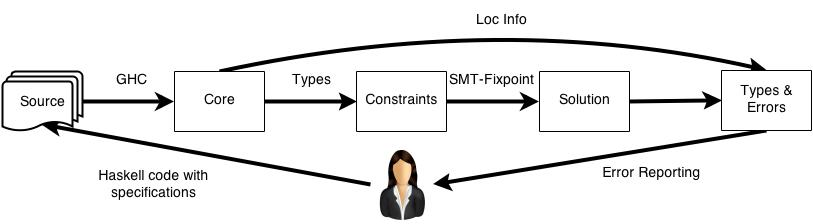
\includegraphics[width=\textwidth]{text/realworldhaskell/liquidHaskell}}
\caption{\toolname Workflow}
	\label{fig:internals}
\end{figure*}
% 
% link for workflow
% https://www.draw.io/#G0Bwp_mIorSVqJb2RENnNVWVlQTmc
%
We will start with a short description of the \toolname workflow,
summarized in Figure~\ref{fig:internals}, and continue with an 
example driven overview of how properties are specified
and verified using the tool. 

% \mypara{Usage} 
\mypara{Source}
\toolname can be run from the command-line\footnote{\url{https://hackage.haskell.org/package/liquidhaskell}}
or within a web-browser\footnote{\url{http://goto.ucsd.edu/liquid/haskell/demo/}}.
It takes as \emph{input}:
%
(1)~a single Haskell \emph{source} file with code and refinement
    type specifications including refined datatype definitions, 
    measures (\S~\ref{sec:tool:measures}), predicate and type 
    aliases, and function signatures;
%
(2)~a set of directories containing \emph{imported modules} 
    (including the \verb+Prelude+) which may themselves 
    contain specifications for exported types and functions; and
%
(3)~a set of predicate fragments called \emph{qualifiers},
    which are used to infer refinement types. This set is 
    typically empty as the default set of qualifiers extracted 
    from the type specifications suffices for inference.

\mypara{Core}
\toolname uses GHC to reduce the source to the Core IL~\cite{SulzmannCJD07}, 
and, to facilitate source-level error reporting, creates a map from Core 
expressions to locations in the Haskell source.

\mypara{Constraints}
Then, it uses the abstract interpretation framework of Liquid Typing~\cite{LiquidPLDI08}, 
modified to ensure soundness under lazy evaluation~\citep{LiquidICFP14},
to generate logical constraints from the Core IL.
     
\mypara{Solution}
Next, it uses a fixpoint algorithm (from~\citep{LiquidPLDI08})
combined with an SMT solver to solve the constraints, and hence 
infers a valid refinement typing for the program. 
%
\toolname can use any solver that implements the SMT-LIB2
standard~\cite{SMTLIB2}, including Z3~\citep{Z3}, CVC4~\citep{CVC4}, and
MathSat~\citep{MathSat}.

 
\mypara{Types \& Errors}
% \NV{satisfiability and validity refer to different things here, 
% which is confusing...}
If the set of constraints is satisfiable, then \toolname outputs 
\textsc{Safe}, meaning the program is verified.
If instead, the set of constraints is not satisfiable, then \toolname
outputs \textsc{Unsafe}, and uses the invalid constraints to 
report refinement type errors at the \emph{source positions}
that created the invalid constraints, using the location 
information to map the invalid constraints to source positions.
%
In either case, \toolname produces as output a source map
containing the \emph{inferred} types for each program 
expression, which, in our experience, is crucial for 
debugging the code and the specifications.

%\mypara{Optional Typing}
%
\toolname is best thought of as an \emph{optional} type checker
for Haskell. By optional we mean that the refinements have \emph{no} 
influence on the dynamic semantics, which makes it easy to apply 
\toolname to \emph{existing} libraries.
%
To emphasize the optional nature of refinements and preserve 
compatibility with existing compilers, all specifications 
appear within comments of the form \verb|{-@ ... @-}|, 
which we omit below for brevity.

\subsection{Specifications}

A refinement type is a Haskell type where each component
of the type is decorated with a predicate from a (decidable)
refinement logic. We use the quantifier-free logic of equality, 
uninterpreted functions and linear arithmetic (QF-EUFLIA)~\cite{Nelson81}. 
For example,
%
\begin{code}
   {v:Int | 0 <= v && v < 100}
\end{code}
%
describes @Int@ values between @0@ and @100@.

\mypara{Type Aliases} For brevity and readability, it is often convenient 
to define abbreviations for particular refinement predicates and types.
For example, we can define an alias for the above predicate
%
\begin{code}
  predicate Btwn Lo N Hi = Lo <= N && N < Hi
\end{code}
%
and use it to define a \emph{type alias}
%
\begin{code}
  type Rng Lo Hi = {v:Int | (Btwn Lo v Hi)} 
\end{code}
%
We can now describe the above integers as @(Rng 0 100)@.

\mypara{Contracts} 
To describe the desired properties of a function, we need
simply refine the input and output types with predicates 
that respectively capture suitable pre- and post-conditions. 
For example,
%
\begin{code}
  range :: lo:Int -> hi:{Int | lo <= hi} 
        -> [(Rng lo hi)]
\end{code}
%
states that @range@ is a function that takes two @Int@s 
respectively named @lo@ and @hi@ and returns a list of @Int@s 
between @lo@ and @hi@. There are three things worth
noting.
%
First, we have binders to name the function's \emph{inputs} 
(\eg, @lo@ and @hi@) and can use the binders inside the 
function's \emph{output}.
%
Second, the refinement in the \emph{input} type describes the 
\emph{pre-condition} that the second parameter @hi@ cannot 
be smaller than the first @lo@.
%
Third, the refinement in the \emph{output} type describes the
\emph{post-condition} that all returned elements are between 
the bounds of @lo@ and @hi@.


\subsection{Verification}\label{sec:tool:verification}

Next, consider the following implementation for @range@:
%
\begin{code}
  range lo hi 
    | lo <= hi  = lo : range (lo + 1) hi
    | otherwise = []
\end{code}
%
When we run \toolname on the above code, it reports an 
error at the definition of @range@. This is unpleasant! 
One way to debug the error is to determine what type has
been \emph{inferred} for @range@, \eg, by hovering the 
mouse over the identifier in the web interface. 
In this case, we see that the output type is essentially:
%
\begin{code}
  [{v:Int | lo <= v && v <= hi}]
\end{code}
%
which indicates the problem. There is an \emph{off-by-one} 
error due to the problematic guard. If we replace the second @<=@ 
with a @<@ and re-run the checker, the function is verified.

\mypara{Holes} It is often cumbersome to specify the Haskell
types, as those can be gleaned from the regular type signatures 
or via GHC's inference. Thus, \toolname allows the user to leave 
holes in the specifications. Suppose @rangeFind@ has type 
%
\begin{code}
  (Int -> Bool) -> Int -> Int -> Maybe Int
\end{code}
%
where the second and third parameters define a range. 
We can give @rangeFind@ a refined specification:
%
\begin{code}
  _ -> lo:_ -> hi:{Int | lo <= hi} 
    -> Maybe (Rng lo hi)
\end{code}
%
where the @_@ is simply the unrefined Haskell type for the 
corresponding position in the type.

\mypara{Inference} Next, consider the implementation
%
\begin{code}
  rangeFind f lo hi = find f $ range lo hi 
\end{code}
%$
where @find@ from @Data.List@ has the (unrefined) type
%
\begin{code}
  find :: (a -> Bool) -> [a] -> Maybe a
\end{code}
%
\toolname uses the abstract interpretation framework of 
Liquid Typing~\cite{LiquidPLDI08} to infer that the type
parameter @a@ of @find@ can be instantiated with @(Rng lo hi)@
thereby enabling the automatic verification of @rangeFind@.

Inference is crucial for automatically synthesizing types
for polymorphic instantiation sites -- note there is another
instantiation required at the use of the apply operator 
@$@ --  and to relieve the programmer of the tedium of %$
specifying signatures for all functions. 
%
Of course, for functions exported by the module,
we must write signatures to specify preconditions -- otherwise, 
the system defaults to using the trivial (unrefined) Haskell 
type as the signature \ie, checks the implementation assuming 
arbitrary inputs.

\subsection{Measures}\label{sec:tool:measures}
%% \NV{DONE(R1)
%% measure is introduced as something that gives the size of a value, 
%% but it is later used for more general properties e.g. almostRB 
%% over red-black trees.
%% }
So far, the specifications have been limited to comparisons and 
arithmetic operations on primitive values. 
We use \emph{measure functions}, or just measures, to 
specify \emph{inductive properties} of algebraic data types. 
%
For example, we define a measure @len@ to write properties about the number
of elements in a list.
%
\begin{code}
  measure len :: [a] -> Int
  len []      = 0
  len (x:xs)  = 1 + (len xs)
\end{code}
%
Measure definitions are \emph{not} arbitrary Haskell code but a very 
restricted subset~\cite{LiquidICFP14}.
Each measure has a single equation per constructor that defines the
value of the measure for that constructor. The right-hand side of the 
equation is a term in the restricted refinement logic. Measures are 
interpreted by generating refinement types for the corresponding 
data constructors.
%
For example, from the above, \toolname derives the 
following types for the list data constructors:
%
\begin{code}
  []  :: {v:[a]| len v = 0}
  (:) :: _ -> xs:_ -> {v:[a]| len v = 1 + len xs}
\end{code}
%
Here, @len@ is an \emph{uninterpreted function} in the refinement logic.
We can define multiple measures for a type; \toolname simply conjoins
the individual refinements arising from each measure to obtain a single
refined signature for each data constructor.

\mypara{Using Measures}
We use measures to write specifications about algebraic types. 
For example, we can specify and verify that: 
%
\begin{code}
  append :: xs:[a] -> ys:[a] 
         -> {v:[a]| len v = len xs + len ys}

  map    :: (a -> b) -> xs:[a] 
         -> {v:[b]| len v = len xs} 

  filter :: (a -> Bool) -> xs:[a] 
         -> {v:[a]| len v <= len xs}
\end{code}

\mypara{Propositions} 
%%In addition to allowing the specification of structural features like
%%lengths, heights and so on, 
Measures can be used to encode sophisticated 
invariants about algebraic data types.
%
To this end, the user can write a measure whose output has a special type 
@Prop@ denoting propositions in the refinement logic. For instance, we can
describe a list that contains a @0@ as:
%
\begin{code}
  measure hasZero :: [Int] -> Prop
  hasZero []      = false
  hasZero (x:xs)  = x == 0 || (hasZero xs) 
\end{code}
%
We can then define lists containing a @0@ as:
%
\begin{code}
  type HasZero = {v : [Int] | (hasZero v)} 
\end{code}
%
Using the above, \toolname will accept 
%
\begin{code}
  xs0 :: HasZero 
  xs0 = [2,1,0,-1,-2]
\end{code}
%
but will reject
%
\begin{code}
  xs' :: HasZero 
  xs' = [3,2,1]
\end{code}



\subsection{Refined Data Types}

Often, we require that \emph{every} instance of a type satisfies some invariants. 
For example, consider a @CSV@ data type, that represents tables:
%
\begin{code}
  data CSV a = CSV { cols :: [String]
                   , rows :: [[a]]    }
\end{code}
%
% With \toolname we can enforce the invariant that for every @CSV@ table, 
% with a number of columns given by @dim@,
% each row has @dim@ elements,
% with the below refined data type definition
%%With \toolname we can enforce the invariant that every @CSV@ table 
%%has the number of columns given by @dim@, and that each row has 
%%@dim@ elements with a refined data type definition, such as:
With \toolname we can enforce the invariant that every row in a @CSV@ table
should have the same number of columns as there are in the header
%
\begin{code}
  data CSV a = CSV { cols :: [String]  
                   , rows :: [ListL a cols] }
\end{code}
%
using the alias
%
\begin{code}
  type ListL a X = {v:[a]| len v = len X}
\end{code}
%
A refined data definition is \emph{global} in that \toolname 
will reject any @CSV@-typed expression that does not respect 
the refined definition. For example, both of the below 
%
\begin{code}
  goodCSV = CSV [  "Month", "Days"] 
                [ ["Jan"  , "31"]
                , ["Feb   , "28"]
                , ["Mar"  , "31"] ]

  badCSV  = CSV [  "Month", "Days"] 
                [ ["Jan"  , "31"]
                , ["Feb   , "28"]
                , ["Mar"        ] ]
\end{code}
%
are well-typed Haskell, but the latter is rejected by \toolname.
%
Like measures, the global invariants are enforced by refining 
the constructors' types. 

\subsection{Refined Type Classes}\label{sec:type-classes}

Next, let us see how \toolname supports the verification of
programs that use ad-hoc polymorphism via type classes.
%
While the implementation of each typeclass instance is 
different, there is often a common interface that we 
expect all instances to satisfy.

\mypara{Class Measures}
As an example, consider the class definition
%
\begin{code}
  class Indexable f where
    size :: f a -> Int
    at   :: f a -> Int -> a
\end{code}
%
For safe access, we might require that @at@'s second 
parameter is bounded by the @size@ of the container.
To this end, we define a \emph{type-indexed} 
measure, using the @class measure@ keyword
%
\begin{code}
  class measure sz :: a -> Nat
\end{code}
%
Now, we can specify the safe-access precondition  
independent of the particular instances of @Indexable@:
%
\begin{code}
  class Indexable f where
    size :: xs:_ -> {v:Nat | v = sz xs}
    at   :: xs:_ -> {v:Nat | v < sz xs} -> a
\end{code}

\mypara{Instance Measures}
For each concrete type that instantiates a class, we require 
a corresponding definition for the measure. 
For example, to define lists as an instance of @Indexable@, 
we require the definition of the @sz@ instance for lists:
%
\begin{code}
  instance measure sz :: [a] -> Nat
  sz []     = 0
  sz (x:xs) = 1 + (sz xs)
\end{code}
%
Class measures work just like regular measures in that the above 
definition is used to refine the types of the list data constructors.
After defining the measure, we can define the type instance as:
%
\begin{code}
  instance Indexable [] where
    size []        = 0
    size (x:xs)    = 1 + size xs

    (x:xs) `at` 0  = x
    (x:xs) `at` i  = index xs (i-1)
\end{code}
%
\toolname uses the definition of @sz@ for lists to check that @size@ 
and @at@ satisfy the refined class specifications. 
% NV the dictionary relevant this were removed
% , and hence, that 
% the above creates a valid instance dictionary for @Indexable@.

\mypara{Client Verification}
At the clients of a type-class we use the refined 
types of class methods. Consider a client of @Indexable@s:
%
\begin{code}
  sum :: (Indexable f) => f Int -> Int
  sum xs = go 0 
    where
      go i | i < size xs = xs `at` i + go (i+1)
           | otherwise   = 0
\end{code}
%
\toolname proves that each call to @at@ is safe, by using the refined
class specifications of @Indexable@. 
Specifically, each call to @at@ is guarded by a check @i < size xs@
and @i@ is  increasing 
from 0, so \toolname proves that @xs `at` i@ will always be safe.

\subsection{Abstracting Refinements}

So far, all the specifications have used \emph{concrete} refinements. Often it is
useful to be able to \emph{abstract} the refinements that appear in a
specification. For example, consider a monomorphic variant of @max@
%
\begin{code}
  max     :: Int -> Int -> Int 
  max x y = if x > y then x else y
\end{code}
%
We would like to give @max@ a specification that lets us verify:
%
\begin{code}
  xPos  :: {v: _ | v > 0}
  xPos  = max 10 13

  xNeg  :: {v: _ | v < 0}
  xNeg  = max (-5) (-8)

  xEven :: {v: _ | v mod 2 == 0} 
  xEven = max 4 (-6)
\end{code}
%
To this end, \toolname allows the user to \emph{abstract refinements} over
types~\cite{vazou13}, for example by typing @max@ as:
%
\begin{code}
 max :: forall <p :: Int -> Prop>. 
          Int<p> -> Int<p> -> Int<p>
\end{code}
%
The above signature states that for any refinement @p@, if the two
inputs of @max@ satisfy @p@ then so does the output. \toolname uses
Liquid Typing to automatically instantiate @p@ with suitable concrete
refinements, thereby checking @xPos@, @xNeg@, and @xEven@.


\mypara{Dependent Composition}
Abstract refinements turn out to be a surprisingly expressive and 
useful specification mechanism. For example, consider the function 
composition operator:
%
\begin{code}
  (.) :: (b -> c) -> (a -> b) -> a -> c
  (.) f g x = f (g x)  
\end{code}
%
Previously, it was not possible to check, \eg that:
%
\begin{code}
  plus3 :: x:_ -> {v:_ | v = x + 3}
  plus3 = (+ 1) . (+ 2)
\end{code}
%
as the above required tracking the dependency between @a@, @b@ and @c@,
which is crucial for analyzing idiomatic Haskell.
With abstract refinements, we can give the @(.)@ operator the type:
%
\begin{code}
  (.) :: forall < p :: b -> c -> Prop
                , q :: a -> b -> Prop>.
           f:(x:b -> c<p x>) 
        -> g:(x:a -> b<q x>) 
        -> y:a 
        -> exists[z:b<q y>].c<p z>
\end{code}
%
which gets automatically instantiated at usage sites, allowing \toolname
to precisely track invariants through the use of the ubiquitous 
higher-order operator.

\mypara{Dependent Pairs}
Similarly, we can abstract refinements over the definition of datatypes.
% Similarly, we can abstract refinements over the definition of datatypes.
For example, we can express dependent pairs in \toolname by refining the 
definition of tuples as:
%
\begin{code}
  data Pair a b <p :: a -> b -> Prop> 
    = Pair { fst :: a, snd :: b<p fst>}
\end{code}
%
That is, the refinement @p@ relates the @snd@ element with the @fst@.
Now we can define increasing and decreasing pairs
%
\begin{code}
  type IncP = Pair <{\x y -> x < y}> Int Int
  type DecP = Pair <{\x y -> x > y}> Int Int
\end{code}
%
and then verify that:
%
\begin{code}
  up :: IncP
  up = Pair 2 5
  
  dn :: DecP
  dn = Pair 5 2
\end{code}
%
Now that we have a bird's eye view of the various specification mechanisms
supported by \toolname, let us see how we can profitably apply them to
statically check a variety of correctness properties in real-world codes.

%%% Local Variables: 
%%% mode: latex
%%% TeX-master: "main"
%%% End: 

\section{Totality}\label{sec:totality}
%% OK \NV{DONE intro (R1)
%% OK Sections 3 and 4 cover "totality" and "termination" respectively. It would be helpful to explain these terms at the start of section 3, so that the two are distinguished appropriately.
%% OK }
Well typed Haskell code can go very wrong:
%
\begin{code}
  *** Exception: Prelude.head: empty list
\end{code}
%
As our first application, let us see how to use 
\toolname to statically guarantee the absence
of such exceptions, \ie, to prove various 
functions \emph{total}.

\subsection{Specifying Totality}

First, let us see how to specify the notion of
totality inside \toolname. Consider the source of 
the above exception:
%
\begin{code}
  head :: [a] -> a
  head (x:_) = x
\end{code}
%
Most of the work towards totality checking is done by 
the translation to GHC's Core, in which every function 
\emph{is} total, but may explicitly call an \emph{error} 
function that takes as input a string that describes the 
source of the pattern-match failure and throws an exception.
%
For example @head@ is translated into
%
\begin{code}
  head d = case d of 
             x:xs -> x
             []   -> patError "head"
\end{code}

Since every core function is total, but may explicitly 
call error functions, to prove that the source function is 
total, it suffices to prove that @patError@ 
will \emph{never} be called.
%
We can specify this requirement by giving the error 
functions a @false@ pre-condition:
%
\begin{code}
  patError :: {v:String | False } -> a
\end{code}
%
The pre-condition states that the input type is \emph{uninhabited}
and so an expression containing a call to @patError@ will only type 
check if the call is \emph{dead code}.


\subsection{Verifying Totality}

The (core) definition of @head@ does not typecheck
as is; but requires a pre-condition that states that the function
is only called with non-empty lists. Formally, we do so by 
defining the alias
%
\begin{code}
  predicate NonEmp X = 0 < len X 
\end{code}
%
and then stipulating that 
%
\begin{code}
  head :: {v : [a] | NonEmp v} -> a
\end{code}
%
To verify the (core) definition of @head@, \toolname uses the above signature
to check the body in an environment
%
\begin{code}
  d :: {0 < len d}
\end{code}
%
When @d@ is matched with @[]@, the environment is 
strengthened with the corresponding refinement from 
the definition of @len@, \ie,
%
\begin{code}
  d :: {0 < (len d) && (len d) = 0}
\end{code}
%
Since the formula above is a contradiction, \toolname concludes that the
call to @patError@ is dead code, and thereby verifies the totality 
of @head@. Of course, now we have pushed the burden of proof onto clients
of @head@ -- at each such site, \toolname will check that the argument 
passed in is indeed a @NonEmp@ list, and if it successfully does so, then
we, at any uses of @head@, can rest assured that @head@ will never throw an 
exception. 

\mypara{Refinements and Totality} 
While the @head@ example is quite simple, in general, refinements make
it easy to prove totality in complex situations, where we must track
dependencies between inputs and outputs. For example, consider the @risers@
function from \cite{catch}:
%
\begin{code}
  risers []       = []
  risers [x]      = [[x]]
  risers (x:y:zs) 
    | x <= y      = (x:s) : ss 
    | otherwise   = [x] : (s:ss) 
    where 
      s:ss    = risers (y:etc)
\end{code}
%
The pattern match on the last line is partial; its core translation is
%
\begin{code}
  let (s, ss) = case risers (y:etc) of
                  s:ss -> (s, ss)
                  []   -> patError "..."
\end{code}
%
What if @risers@ returns an empty list? 
Indeed, @risers@ \emph{does}, on occasion, return an empty list per its
first equation. However, on close inspection, it turns out that 
\emph{if} the input is non-empty, \emph{then} the output is also
non-empty. Happily, we can specify this as:
%
\begin{code}
  risers :: l:_ -> {v:_ | NonEmp l => NonEmp v} 
\end{code}

\toolname verifies that @risers@ meets the above specification, 
and hence that the @patError@ is dead code as at that 
site, the scrutinee is obtained from calling @risers@ with a
@NonEmp@ list.

\mypara{Non-Emptiness via Measures}
Instead of describing non-emptiness indirectly using @len@, a 
user could a special measure:
%
\begin{code}
  measure nonEmp  :: [a] -> Prop
  nonEmp (x:xs)   = True
  nonEmp []       = False

  predicate NonEmp X = nonEmp X
\end{code}
%
After which, verification would proceed analagous to the above.

\mypara{Total Totality Checking} 
@patError@ is one of many possible errors thrown by non-total functions.  
@Control.Exception.Base@ has several others including @recSelError@, @irrefutPatError@, \etc which serve the purpose of making 
core translations total.
%
Rather than hunt down and specify @False@ preconditions one
by one, the user may automatically turn on totality checking 
by invoking \toolname with the \cmdtotality command line option, 
at which point the tool systematically checks that all the above 
functions are indeed dead code, and hence, that all definitions are total.

\subsection{Case Studies}

We verified totality of two libraries: \lbhscolour and \lbmap, earlier versions
of which had previously been proven total by \texttt{catch}~\citep{catch}.

\mypara{\lbmap} 
is a widely used library for (immutable) key-value maps, implemented
as balanced binary search trees.
Totality verification of \lbmap was quite straightforward.
We had already verified termination and the crucial 
binary search invariant~\ref{chapter:abstractrefinements}. To verify 
totality it sufficed to simply re-run verification with
the \cmdtotality argument.
%
All the important specifications were already captured by the types, 
and no additional changes were needed to prove totality.
%
%% \RJ{was it trivially total? i.e. is it total if you strip out all refinements
%% from specs?}
%% \NV{No, it fails in 6 functions all of which can trivially be reasoned to be total}
%% \NV{hedgeUnion, hedgeDiff, hedgeMerge, submap', join, merge}
%% \NV{The interesting story is that during verification \emph{we accidentally modified}
%% turn a function to partial, see my commit 041f1f0fea4d34ee41f50dbf7ce43e3c084c2743}
%

This case study illustrates an advantage of \toolname over specialized provers 
(\eg, \texttt{catch}~\citep{catch}): it can be used to prove totality, termination and
functional correctness at the same time, facilitating a nice reuse of
specifications for multiple tasks.

%% DONE \NV{(R3)
%% DONE Before discussing HsColour, I'd give a brief explanation of what it is.
%% DONE }
\mypara{\lbhscolour} is a library for generating syntax-highlighted LATEX and HTML from
Haskell source files.
Checking \lbhscolour was not so easy, as in some cases assumptions are used about the 
structure of the input data:
%
For example, @ACSS.splitSrcAndAnnos@ handles an
input list of @String@s and assumes that whenever
a specific @String@ (say @breakS@) appears then 
at least two @String@s (call them @mname@ and @annots@)
follow it in the list.
Thus, for a list @ls@ that starts with @breakS@ 
the irrefutable pattern  @(_:mname:annots)@ @=@ @ls@
should be total.
%
Though possible, it is currently it is somewhat cumbersome to specify such 
properties. 
%
As an easy and practical solution, 
to prove totality, we added a dynamic check that 
validates that the length of the input @ls@ exceeds @2@.

%% measure follows a b c = \case 
%%   []   -> true
%%   x:xs -> if x == a then first2 b c xs else follows a b c xs
%% 
%% measure first2 b c = \case
%%   []   -> false
%%   x:xs -> x == b && first1 c xs
%% 
%% measure first1 c = \case
%%   []   -> false
%%   x:xs -> x == c
%% 
%% Worse, \toolname has no way to express such an invariant: 
%% \toolname naturally describes invariants that recursively 
%% hold for every list element and 
%% reaches its limitations when reasoning about non-recursive
%% properties.

In other cases assertions were imposed via monadic checks, \eg @HsColour.hs@ reads the input arguments and 
checks their well-formedness using 
%
\begin{code}
  when (length f > 1) $ errorOut "..."
\end{code} %$
%
Currently \toolname does not support monadic reasoning that 
allows assuming that @(length f <= 1)@
holds when executing the action \emph{following} the @when@ check. 
%
Finally, code modifications were required to capture properties 
that are cumbersome to express with \toolname.
%
For example, @trimContext@ checks if there is an element that 
satisfies @p@ in the list @xs@; if so it defines 
%
@ys = dropWhile (not . p) xs@
%
and computes @tail ys@.
%
By the check we know that @ys@ has at least one element, the 
one that satisfies @p@. 
%
Due to the complexity of this property, we preferred to rewrite the specific code 
in a more verification friendly version. 


%%% \mynote{Bug}
%%% %
%%% \RJ{WHY? Seems like a simple GHC CHECK?}
%%% %
%%% On the positive side, totality verification revealed a subtle bug:
%%% %
%%% The instance @Enum@ of @Highlight@ does not define the @toEnum@ 
%%% method. In core, this reduces to a call to the error function 
%%% @noMethodBinding@.
%%% %
%%% Even though this totality bug can be tracked by GHC compilation,
%%% it exposes the strengths of our totality checker.

On the whole, while proving totality can be cumbersome 
(as in \lbhscolour) it is a nice side benefit of refinement
type checking and can sometimes be a fully automatic corollary
of establishing more interesting safety properties (as in \lbmap).

\section{Termination}\label{sec:termination}

To soundly account for Haskell's non-strict evaluation, a refinement
type checker must distinguish between terms that may potentially 
diverge and those that will not~\cite{LiquidICFP14}.
%
Thus, by default, \toolname proves termination of each recursive function.
Fortunately, refinements make this onerous task quite straightforward. 
We need simply associate a \emph{well-founded termination metric} % $\mu$
on the function's parameters, and then use refinement typing to check 
that the metric strictly decreases at each recursive call. In practice,
due to a careful choice of defaults, this amounts to about a line 
of termination-related hints per hundred lines of source. 
Details about the termination checker may be found in \cite{LiquidICFP14}, 
we include a brief description here to make the paper self-contained.

\mypara{Simple Metrics}
As a starting example, consider the @fac@ function
%
\begin{code}
  fac :: n:Nat -> Nat / [n]
  fac 0 = 1 
  fac n = n * fac (n-1)
\end{code}
%
The termination metric is simply the parameter @n@; 
as @n@ is non-negative and decreases at the recursive 
call, \toolname verifies that @fac@ will terminate.
%
We specify the termination metric in the type signature 
with the @/[n]@.

Termination checking is performed at the same 
time as regular type checking, as it can be 
reduced to refinement type checking with a 
special terminating fixpoint combinator~\cite{LiquidICFP14}.
Thus, if \toolname fails to prove that a given 
termination metric is well-formed and decreasing, 
it will report a @Termination Check@ @Error@. 
%% \RJ{Seems untrue -- I just get a plain old liquid type error?
%% NV: IF you provide termination metrics, you DO get termination check error}.
At this point, the user can either debug 
the specification, or mark the function 
as non-terminating.


%%\mypara{Refinements Enable Termination} 
%%Consider Euclid's GCD:
%%%
%%\begin{code}
%%  gcd :: a:Nat -> {v:Nat | v < a} -> Nat 
%%  gcd a 0 = a
%%  gcd a b = gcd b (a `mod` b)
%%\end{code}
%%%
%%Here, the termination metric is the first parameter @a@.
%%To prove that @a@ is decreasing requires
%%the fact that the second parameter is smaller than the first 
%%and that @mod@ returns results smaller than its second 
%%parameter. Both facts are easily expressed as refinements, 
%%but elude non-extensible checkers~\cite{Giesl11}.
%%
%%\mypara{Explicit Termination Metrics}
%%The termination metric can be some parameter \emph{other} than the first 
%%argument.
%%For example, consider: % As an example, consider the tail-recursive factorial:
%%%
%%\begin{code}
%%  tfac     :: Nat -> n:Nat -> Nat / [n] 
%%  tfac x 0 = if n == 0 then x
%%                       else tfac (n*x) (n-1)
%%\end{code}
%%%
%%%
%%It can be checked that @n@, \ie, the second argument is decreasing at each recursive call.
%%
\mypara{Termination Expressions} 
Sometimes, no single parameter decreases across recursive calls,
but there is some \emph{expression} that forms the decreasing 
metric.
%
For example recall @range lo hi@ (from \S~\ref{sec:tool:verification}) 
which returns the list of @Int@s from @lo@ to @hi@:
%
\begin{code}
  range lo hi 
    | lo < hi   = lo : range (lo+1) hi
    | otherwise = [] 
\end{code}
%
Here, neither parameter is decreasing (indeed, the first 
one is increasing) but @hi-lo@ decreases across each call. 
To account for such cases, we can specify as the termination
metric a (refinement logic) expression over the function
parameters. Thus, to prove termination, we could type @range@ as:
\begin{code}
  lo:Int -> hi:Int -> [(Btwn lo hi)] / [hi-lo]
\end{code}

\mypara{Lexicographic Termination}
The Ackermann function
%
\begin{code}
  ack m n 
    | m == 0    = n + 1
    | n == 0    = ack (m-1) 1 
    | otherwise = ack (m-1) (ack m (n-1))
\end{code}
%
is curious as there exists no simple, natural-valued, 
termination metric that decreases at each recursive call.
%
However @ack@ terminates because at each call \emph{either}
@m@ decreases \emph{or} @m@ remains the same and @n@ decreases. 
%
In other words, the pair @(m,n)@ strictly decreases according to a
\emph{lexicographic} ordering. 
%
Thus \toolname supports termination metrics that are a 
\emph{sequence of} termination expressions. For example, 
we can type @ack@ as:
%
\begin{code}
  ack :: m:Nat -> n:Nat -> Nat / [m, n]
\end{code}
%
At each recursive call \toolname uses a lexicographic 
ordering to check that the sequence of termination 
expressions is decreasing (and well-founded in each component).

\mypara{Mutual Recursion}
%
The lexicographic mechanism lets us check termination of
mutually recursive functions, \eg @isEven@ and @isOdd@
%
\begin{code}
  isEven 0 = True
  isEven n = isOdd $ n-1
  
  isOdd n  = not $ isEven n 
\end{code}
%
Each call terminates as either @isEven@ calls @isOdd@ with a 
decreasing parameter, \emph{or} @isOdd@ calls @isEven@ with 
the same parameter, expecting the latter to do the decreasing.
%
For termination, we type:
%
\begin{code}
  isEven :: n:Nat -> Bool / [n, 0]
  isOdd  :: n:Nat -> Bool / [n, 1]
\end{code}
%
To check termination, \toolname verifies that at each recursive 
call the metric of the caller is less than the metric of the 
callee.
%
When @isEven@ calls @isOdd@, it proves that the caller's 
metric, namely @[n,0]@ is greater than the callee's @[n-1,1]@.
When \hbox{@isOdd@} calls @isEven@, it proves that the 
caller's metric @[n,1]@ is greater than the callee's @[n,0]@,
thereby proving the mutual recursion always terminates.

\mypara{Recursion over Data Types}
The above strategies generalize easily to functions that recurse
over (finite) data structures like arrays, lists, and trees.
In these cases, we simply use \emph{measures} to project the 
structure onto @Nat@, thereby reducing the verification to 
the previously seen cases. 
For example, we can prove that @map@ 
%
\begin{code}
  map f (x:xs) = f x : map f xs
  map f []     = []
\end{code}
%
terminates, by typing @map@ as 
%
\begin{code}
  (a -> b) -> xs:[a] -> [b] / [len xs]
\end{code}
%
\ie, by using the measure @len xs@, from \S~\ref{sec:tool:measures}, 
as the metric.

%%% %
%%% \begin{code}
%%%   data L [sz] a = N | C a (L a)
%%% \end{code}
%%% %
%%% we can define a \emph{measure}
%%% %
%%% \begin{code}
%%%   measure sz  :: L a -> Nat
%%%   sz (C x xs) = 1 + (sz xs)
%%%   sz N        = 0
%%% \end{code}
%%% %
%%% We prove that @map@ terminates using the type:
%%% %
%%% \begin{code}
%%%   map :: (a -> b) -> xs:L a -> L b / [sz xs]
%%%   map f (C x xs) = C (f x) (map f xs)
%%%   map f N        = N
%%% \end{code}
%%% %
%%% That is, by simply using @(sz xs)@  as the 
%%% decreasing metric.

\mypara{Generalized Metrics Over Datatypes}
In many functions there is no single argument 
whose measure provably decreases. Consider
%
\begin{code}
  merge (x:xs) (y:ys)
    | x < y     = x : merge xs (y:ys)
    | otherwise = y : merge (x:xs) ys
\end{code}
%
from the homonymous sorting routine. Here, neither
parameter decreases, but the \emph{sum} of their 
sizes does. To prove termination, we can type @merge@ as:
%
\begin{code}
  xs:[a] -> ys:[a] -> [a] / [len xs + len ys]
\end{code}

%%%% \begin{figure*}[!t]
%%%% 	\begin{code}
%%%% 	type OL  a   =  [a]<{\fld v -> (v >= fld)}>
%%%% 
%%%% 	qsort :: (Ord a) => xs:[a] -> OL a / [(len xs), 0]
%%%% 	qsort []         = []
%%%% 	qsort (x:xs)     = qpart x xs [] []
%%%% 
%%%% 	qpart :: (Ord a) => x:a -> q:[a] -> r: [{v:a|v<x}] -> p: [{v:a|v>=x}] -> OL a 
%%%% 	       / [((len q) + (len r) + (len p)), ((len q) + 1)]
%%%% 	qpart x []     rlt rge             = app x (qsort rlt) (x:qsort rge)
%%%% 	qpart x (y:ys) rlt rge | x > y     = qpart x ys (y:rlt) rge
%%%% 	                       | otherwise = qpart x ys rlt (y:rge)
%%%% 
%%%% 	app k []     ys = ys
%%%% 	app k (x:xs) ys = x : (app k xs ys)
%%%% 	\end{code}
%%%% \caption{Mutual-recursive qsort}
%%%% \label{fig:code:qsort}
%%%% \end{figure*}


\mypara{Putting it all Together}
The above techniques can be combined to prove 
termination of the mutually recursive quick-sort (from~\citep{XiTerminationLICS01})% \RJ{from where?}
%
\begin{code}
  qsort (x:xs)   = qpart x xs [] []
  qsort []       = []

  qpart x (y:ys) l r 
    | x > y      = qpart x ys (y:l) r 
    | otherwise  = qpart x ys l (y:r)
  qpart x [] l r = app x (qsort l) (qsort r) 

  app k []     z = k : z
  app k (x:xs) z = x : app k xs z
\end{code}
%
@qsort (x:xs)@ calls @qpart x xs@ to partition @xs@ 
into two lists @l@ and @r@ that have elements less 
and greater or equal than the pivot @x@, respectively.
%
When @qpart@ finishes partitioning it mutually recursively
calls @qsort@ to sort the two list and appends the results 
with @app@. 
%
\toolname proves sortedness as well~\cite{vazou13} but let us 
focus here on termination. To this end, we type the functions
as:
%
\begin{code}
  qsort :: xs:_ -> _ 
        / [len xs, 0]
    
  qpart :: _ -> ys:_ -> l:_ -> r:_ -> _ 
        / [len ys + len l + len r, 1 + len ys]
\end{code}
%
As before, \toolname checks that at each recursive call 
the caller's metric is less than the callee's. 
%
When @qsort@ calls @qpart@ the length of the unsorted 
list @len (x:xs)@ exceeds the \hbox{@len xs + len [] + len []@}.
%
When @qpart@ recursively calls itself the first component
of the metric is the same, but the length of the unpartitioned 
list decreases, \ie @1 + len y:ys@ exceeds \hbox{@1 + len ys@}.
%
Finally, when @qpart@ calls @qsort@ we have \hbox{@len ys + len l + len r@}
exceeds both @len l@ and @len r@, thereby ensuring termination.


%%% Before we dive into proving termination, note that the 
%%% type alias @OL a@ uses Abstract Refinements~\citep{vazou13} to describe 
%%% Ordered Lists. 
%%% Thus, when \toolname decides that the @qsort@ is SAFE, 
%%% it proves both termination and sortedness.
%%%%Note that classical appending @rlt ++ rge@ of the two sorted lists will lose 
%%%%the crucial for sorting information that every element of @rlt@ is less than each element of @rge@.
%%%%%
%%%%Thus we defined a new version of list appending @app@ that uses the pivot element @k@
%%%%as a ghost-parameter.
%%%%%
%%%%Good news is that \toolname will automatically infer the appropriate type of @app@!

%% Let \mus{xs} and \mup{q}{r}{p} be the (well-founded) termination pairs
%% for @qsort xs@ and @qpart x q r p@ respectively, as annotated in the type signatures.
%% %
%%%$\mu_s(x:xs) = (1 + len xs, 0) > (len xs + 0 + 0, len xs + 1) = \mu_p(xs, [], [])$
%%%$\mu_p(y:ys, rlt, rge) = ((1 + (len ys)) + (len rlt) + (len rge), (1 + len ys) + 1) > 
%%%(len ys + (1 + (len rlt)) + (len rge), ((len ys) + 1)) = \mu_p(ys, y:rlt, rge) $
%%%$\mu_p([], rlt, rge) = (0 + len rlt + len rge, 1) > (len rlt, 0) = \mu_s(rlt)$ 

%% Existing techniques~\citep{CookPR11} could be used to 
%% come up with termination metrics.
%% We leave embedding these techniques into \toolname as a future work, and instead
%% we use some defaults to automate termination proving 
%% on functions with trivial metrics.

\mypara{Automation: Default Size Measures}
%
The @qsort@ example illustrates that while \toolname is 
very expressive, devising appropriate termination metrics 
can be tricky.
%
Fortunately, such patterns are very uncommon, and the vast
majority of cases in real world programs are just structural 
recursion on a datatype.
%
\toolname automates termination proofs for this common case,
by allowing users to specify a \emph{default size measure} 
for each data type, \eg @len@ for @[a]@.
%
Now, if no explicit termination metric is given, by default 
\toolname assumes that the \emph{first} argument whose type
has an associated size measure decreases.
%
Thus, in the above, we need not specify metrics for @fac@ 
or @map@ as the size measure is automatically 
used to prove termination. 
%
This heuristic suffices to \emph{automatically}
prove 67\% of recursive functions terminating.

\mypara{Disabling Termination Checking}
In \texttt{Haskell}'s lazy setting not all functions are terminating.
% 
\toolname provides two mechanisms the disable termination proving.
%
A user can disable checking a single function by marking 
that function as lazy. For example, specifying @lazy repeat@ 
tells the tool to not prove @repeat@ terminates.
%
Optionally, a user can disable termination checking for a whole
module by using the command line argument \cmdnotermination
for the entire file.

\section{Memory Safety}\label{sec:memory-safety}

The terms ``Haskell'' and ``pointer arithmetic'' rarely occur in the same
sentence, yet many Haskell programs are constantly manipulating pointers under
the hood by way of using the \bytestring and \libtext libraries. These libraries
sacrifice safety for (much needed) speed and are therefore natural candidates for
verification through \toolname.

\subsection{Bytestring}\label{sec:bytestring}
The single most important aspect of the \bytestring 
library, %~\cite{bytestring}, 
our first case study, is its pervasive intermingling of
high level abstractions like higher-order loops,
folds, and fusion, with low-level pointer 
manipulations in order to achieve high-performance. 
%
%% From the package description, \bytestring is, 
%% ``A time and space-efficient implementation of byte vectors using packed
%% Word8 arrays, suitable for high performance use, both in terms of large
%% data quantities, or high speed requirements. Byte vectors are encoded as
%% strict Word8 arrays of bytes, held in a ForeignPtr, and can be passed
%% between C and Haskell with little effort."
%
\bytestring is an appealing target for evaluating
\toolname, as refinement types are an ideal way to 
statically ensure the correctness of the delicate 
pointer manipulations, errors in which lie below 
the scope of dynamic protection.

The library spans $8$ files (modules) totaling about 3,500 lines.
We used \toolname to verify the library by giving precise 
types describing the sizes of internal pointers and bytestrings. 
These types are used in a modular fashion to verify the 
implementation of functional correctness properties of 
higher-level API functions which are built using 
lower-level internal operations. 
Next, we show the key invariants and how
\toolname reasons precisely about pointer
arithmetic and higher-order codes.

\spara{Key Invariants}
A (strict) @ByteString@ is a triple of a @pay@load pointer, 
an @off@set into the memory buffer referred to by the pointer 
(at which the string actually ``begins") and a @len@gth 
corresponding to the number of bytes in the string, which is 
the size of the buffer \emph{after} the @off@set, that
corresponds to the string.
%
We define a measure for the \emph{size} of 
a @ForeignPtr@'s buffer, and use it to define 
the key invariants as a refined datatype 
%
\begin{code}
  measure fplen  :: ForeignPtr a -> Int
  data ByteString = PS 
     { pay :: ForeignPtr Word8
     , off :: {v:Nat | v       <= fplen pay }
     , len :: {v:Nat | off + v <= fplen pay } }
\end{code}
%
The definition states that 
the offset is a @Nat@ no bigger than the size of 
the @payload@'s buffer, and that
the sum of the @off@set and non-negative @len@gth
is no more than the size of the payload buffer.
Finally, we encode a @ByteString@'s size as a measure.
%
\begin{code}
  measure bLen   :: ByteString -> Int
  bLen (PS p o l) = l
\end{code}

\spara{Specifications}
We define a type alias for a @ByteString@ whose length is the same
as that of another, and use the alias to type the API 
function @copy@, which clones @ByteString@s.

\begin{code}
  type ByteStringEq B = {v:ByteString | (bLen v) = (bLen B)}
  
  copy :: b:ByteString -> ByteStringEq b 
  copy (PS fp off len) 
    = unsafeCreate len $ \p -> 
        withForeignPtr fp $ \f ->
          memcpy len p (f `plusPtr` off) 
\end{code}

\spara{Pointer Arithmetic}
The simple body of @copy@ abstracts a fair bit of internal work. 
@memcpy sz dst src@, implemented in \C and accessed via the FFI is a potentially
dangerous, low-level operation, that copies @sz@ bytes starting
\emph{from} an address @src@ \emph{into} an address @dst@. 
Crucially, for safety, the regions referred to be @src@ and @dst@ 
must be larger than @sz@. We capture this requirement by defining
a type alias @PtrN a N@ denoting GHC pointers that refer to a region
bigger than @N@ bytes, and then specifying that the destination
and source buffers for @memcpy@ are large enough. 

\begin{code}
  type PtrN a N = {v:Ptr a | N <= (plen v)}
  memcpy :: sz:CSize -> dst:PtrN a siz 
                     -> src:PtrN a siz 
                     -> IO () 
\end{code}


The actual output for @copy@ is created and filled in using the 
internal function @unsafeCreate@ which is a wrapper around. 
% -- | Create ByteString of size @l@ and use
% --   action @f@ to fill it's contents.
\begin{code}
  create :: l:Nat -> f:(PtrN Word8 l -> IO ())
         -> IO (ByteStringN l)
  create l f = do
      fp <- mallocByteString l
      withForeignPtr fp $ \p -> f p
      return $! PS fp 0 l
\end{code}

% We include the comment to illustrate how the 
% refinement type captures the natural language 
% requirement in a machine checkable manner.
%
The type of @f@ specifies that the action
will only be invoked on a pointer of length at least 
@l@, which is verified by propagating the types of
@mallocByteString@ and @withForeignPtr@. 
%
The fact that the action is only invoked on such pointers 
is used to ensure that the value @p@ in the body of @copy@ 
is of size @l@. This, and the @ByteString@ 
invariant that the size of the payload @fp@ 
exceeds the sum of @off@ and @len@, ensures 
safety of the @memcpy@ call.

\spara{Interfacing with the Real World}
The above illustrates how \toolname analyzes code that interfaces 
with the ``real world" via the \C FFI. We specify the behavior 
of the world via a refinement typed interface. These types are then assumed
to hold for the corresponding functions, \ie generate pre-condition checks
and post-condition guarantees at usage sites within the Haskell code.


\spara{Higher Order Loops} 
@mapAccumR@ combines a @map@ and a @foldr@ over a @ByteString@. 
The function uses non-trivial recursion, and demonstrates 
the utility of abstract-interpretation based inference. 
%
\begin{code}
  mapAccumR f z b = unSP $ loopDown (mapAccumEFL f) z b
\end{code}
%$
To enable fusion \cite{streamfusion} 
@loopDown@ uses a higher order @loopWrapper@ 
to iterate over the buffer with a @doDownLoop@ action:
%
%% DONE \ES{should we use a termination expression for ``loop'' even though it won't actually work atm in LH?}
\begin{code}
  doDownLoop f acc0 src dest len = loop (len-1) (len-1) acc0
    where
     loop :: s:_ -> _ -> _ -> _ / [s+1]
     loop s d acc 
       | s < 0 
       = return (acc :*: d+1 :*: len - (d+1))
       | otherwise       
       = do x <- peekByteOff src s
            case f acc x of
              (acc' :*: NothingS) -> 
                   loop (s-1) d acc'
              (acc' :*: JustS x') -> 
                   pokeByteOff dest d x'
                >> loop (s-1) (d-1) acc'
\end{code}

The above function iterates across the @src@ and @dst@ 
pointers from the right (by repeatedly decrementing the 
offsets @s@ and @d@ starting at the high @len@ down to @-1@). 
Low-level reads and writes are carried out using the 
potentially dangerous @peekByteOff@ and @pokeByteOff@ 
respectively. To ensure safety, we type these low level 
operations with refinements stating that they are only 
invoked with valid offsets @VO@ into the input buffer @p@.

\begin{code}
  type VO P    = {v:Nat | v < plen P}
  peekByteOff :: p:Ptr b -> VO p -> IO a
  pokeByteOff :: p:Ptr b -> VO p -> a -> IO ()
\end{code}

The function @doDownLoop@ is an internal function.
Via abstract interpretation~\cite{LiquidPLDI08}, 
\toolname infers that
%
(1)~@len@ is less than the sizes of @src@ and @dest@,
(2)~@f@ (here, @mapAccumEFL@) always returns a @JustS@, so
(3)~source and destination offsets satisfy $\mathtt{0 \leq s, d < {len}}$,
(4)~the generated @IO@ action returns a triple @(acc :*: 0 :*: len)@,
%
thereby proving the safety of the accesses in @loop@ \emph{and}
verifying that @loopDown@ and the API function @mapAccumR@ 
return a \bytestring whose size equals its input's.
 
To prove \emph{termination}, we add a \emph{termination expression} 
@s+1@ which is always non-negative and decreases at each call.

\spara{Nested Data}
@group@ splits a string like @"aart"@ into the list
@["aa","r","t"]@, \ie a list of
(a)~non-empty @ByteString@s whose 
(b)~total length equals that of the input. 
To specify these requirements, we define a measure for 
the total length of strings in a list and use it to
define the list of \emph{non-empty} strings
whose total length equals that of another string:

\begin{code}
  measure bLens :: [ByteString] -> Int 
  bLens ([])     = 0
  bLens (x:xs)   = bLen x + bLens xs
  
  type ByteStringNE    = {v:ByteString | bLen v > 0}
  type ByteStringsEq B = {v:[ByteStringNE] | bLens v = bLen b}
\end{code}
%
\toolname uses the above to verify that
%
\begin{code}
  group :: b:ByteString -> ByteStringsEq b
  group xs
   | null xs   = []
   | otherwise = let x        = unsafeHead xs
                     xs'      = unsafeTail xs
                     (ys, zs) = spanByte x xs' 
                 in (y `cons` ys) : group zs
\end{code}
%
The example illustrates why refinements are critical for
proving termination. \toolname determines that @unsafeTail@ 
returns a \emph{smaller} @ByteString@ than its input and that
each element returned by @spanByte@ is no bigger than the 
input, concluding that @zs@ is smaller than @xs@, hence
checking the body under the termination-weakened environment.

To justify the output type, let's look at @spanByte@,
which splits strings into a pair:
%
\begin{code}
  spanByte c ps@(PS x s l) 
    = inlinePerformIO $ withForeignPtr x $
          \p -> go (p `plusPtr` s) 0
    where
      go :: _ -> i:_ -> _ / [l-i]
      go p i 
        | i >= l    = return (ps, empty)
        | otherwise = do
            c' <- peekByteOff p i
            if c /= c'
              then let b1 = unsafeTake i ps
                       b2 = unsafeDrop i ps
                   in  return (b1, b2)
              else go p (i+1)
\end{code}
%
Via inference, \toolname verifies the safety of 
the pointer accesses, and determines that the 
sum of the lengths of the output pair of 
@ByteString@s equals that of the input @ps@.
@go@ terminates as @l-i@ is a well-founded 
decreasing metric.

%%% Local Variables: 
%%% mode: latex
%%% TeX-master: "main"
%%% End: 


\subsection{Text}\label{sec:text}
Next %, to give a qualitative sense of the kinds of properties analyzed 
% during the course of our evaluation, 
we present a brief overview of the verification of \libtext, which 
is the standard library used for serious unicode text processing. 
\libtext uses byte arrays and stream fusion to guarantee 
performance while providing a high-level API.
In our evaluation of \toolname on \libtext,%~\cite{text},
we focused on two types of properties: 
(1) the safety of array index and write operations, and 
(2) the functional correctness of the top-level API.
%
These are both made more interesting by the fact that 
\libtext internally encodes characters using UTF-16, 
in which characters are stored in either two or four bytes.
%
\libtext is a vast library spanning 39 modules and 5,700 lines of
code, however we focus on the 17 modules that are relevant
to the above properties.
%
While we have verified exact functional correctness size properties
for the top-level API, we focus here on the low-level functions 
and interaction with unicode.

\spara{Arrays and Texts}
A @Text@ consists of an (immutable) @Array@ of 16-bit words,
an offset into the @Array@, and a length describing the
number of @Word16@s in the @Text@.  
The @Array@ is created and filled using a
\emph{mutable} @MArray@. 
All write operations in \libtext are performed on @MArray@s 
in the @ST@ monad, but they are \emph{frozen} into @Array@s
before being used by the @Text@ constructor.
%
We write a measure for the size of an @MArray@ and use
it to type the write and freeze operations.
%
\begin{code}
  measure malen       :: MArray s -> Int
  predicate EqLen A MA = alen A = malen MA
  predicate Ok I A     = 0 <= I < malen A
  type VO A            = {v:Int| Ok v A} 
  
  unsafeWrite  :: m:MArray s
               -> VO m -> Word16 -> ST s ()
  unsafeFreeze :: m:MArray s
               -> ST s {v:Array | EqLen v m}
\end{code}

\spara{Reasoning about Unicode}
The function @writeChar@ (abbreviating the function \texttt{unsafeWrite} from \texttt{UnsafeChar})
writes a @Char@ into an @MArray@.
\libtext uses UTF-16 to represent characters internally,
meaning that every @Char@ will be encoded using two or 
four bytes (one or two @Word16@s).
%
\begin{code}
  writeChar marr i c
      | n < 0x10000 = do
          unsafeWrite marr i (fromIntegral n)
          return 1
      | otherwise = do
          unsafeWrite marr i lo
          unsafeWrite marr (i+1) hi
          return 2
      where n = ord c
            m = n - 0x10000
            lo = fromIntegral
               $ (m `shiftR` 10) + 0xD800
            hi = fromIntegral
               $ (m .&. 0x3FF) + 0xDC00
\end{code}
%
The UTF-16 encoding complicates the specification of the function
as we cannot simply require @i@ to be less than the length of 
@marr@; if @i@ were @malen marr - 1@ and @c@ required two 
@Word16@s, we would perform an out-of-bounds write. 
%
We account for this subtlety with a predicate that states 
there is enough @Room@ to encode @c@.
%
% measure ord         :: Char -> Int
\begin{code}
  predicate OkN I A N  = Ok (I+N-1) A
  predicate Room I A C = if ord C < 0x10000
                         then OkN I A 1
                         else OkN I A 2
  
  type OkSiz I A = {v:Nat  | OkN  I A v}
  type OkChr I A = {v:Char | Room I A v}
\end{code}
%
@Room i marr c@ says 
``if @c@ is encoded using one @Word16@, 
  then @i@ must be less than @malen marr@,
  otherwise @i@ must be less than @malen marr - 1@.''
%
@OkSiz I A@ is an alias for a valid number of @Word16@s 
remaining after the index @I@ of array @A@. 
@OkChr@ specifies the @Char@s for which there is room (to write)
at index @I@ in array @A@.
%
The specification for @writeChar@ states that given an array \hbox{@marr@,}
an index @i@, and a valid @Char@ for which there is room at index \hbox{@i@,}
the output is a monadic action returning the number of @Word16@ occupied
by the @char@.
%
\begin{code}
  writeChar :: marr:MArray s
            -> i:Nat
            -> OkChr i marr
            -> ST s (OkSiz i marr)
\end{code}
%
\spara{Bug}
Thus, clients of @writeChar@ should only call it with suitable indices
and characters.
%
Using \toolname we found an error in one client, @mapAccumL@, 
which combines a map and a fold over a @Stream@, and stores 
the result of the map in a @Text@. Consider the inner loop of @mapAccumL@.
%
% \begin{code}
% mapAccumL f z0 (Stream next0 s0 len) =
%   (nz, Text na 0 nl)
%  where
%   mlen = upperBound 4 len
%   (na,(nz,nl)) = runST $ do
%        (marr,x) <- (new mlen >>= \arr ->
%                     outer arr mlen z0 s0 0)
%        arr      <- unsafeFreeze marr
%        return (arr,x)
%   outer arr top = loop
%    where
%     loop !z !s !i =
%       case next0 s of
%         Done          -> return (arr, (z,i))
%         Skip s'       -> loop z s' i
%         Yield x s'
%           | j >= top  -> do
%             let top' = (top + 1) `shiftL` 1
%             arr' <- new top'
%             copyM arr' 0 arr 0 top
%             outer arr' top' z s i
%           | otherwise -> do
%             let (z',c) = f z x
%             d <- writeChar arr i c
%             loop z' s' (i+d)
%           where j | ord x < 0x10000 = i
%                   | otherwise       = i + 1
% \end{code}
\begin{code}
  outer arr top = loop
   where
    loop !z !s !i =
      case next0 s of
        Done          -> return (arr, (z,i))
        Skip s'       -> loop z s' i
        Yield x s'
          | j >= top  -> do
            let top' = (top + 1) `shiftL` 1
            arr' <- new top'
            copyM arr' 0 arr 0 top
            outer arr' top' z s i
          | otherwise -> do
            let (z',c) = f z x
            d <- writeChar arr i c
            loop z' s' (i+d)
          where j | ord x < 0x10000 = i
                  | otherwise       = i + 1
\end{code}
%
Let's focus on the @Yield x s'@ case.
%
We first compute the maximum index @j@ to 
which we will write and determine the safety of a write. 
%
If it is safe to write to @j@ we call the provided 
function @f@ on the accumulator @z@ and the character 
@x@, and write the \emph{resulting} character @c@ into the array. 
%
However, we know nothing about @c@, in particular, 
whether @c@ will be stored as one or two @Word16@s! 
Thus, \toolname flags the call to @writeChar@ as \emph{unsafe}.
The error can be fixed by lifting @f z x@ into the @where@ clause and defining the
write index @j@ by comparing @ord c@ (not @ord x@). \toolname (and the authors)
readily accepted our fix.

%% INCLUDEPROOF To illustrate why the call is in fact buggy, 
%% INCLUDEPROOF consider a sample iteration of @loop@ 
%% INCLUDEPROOF where @i = malen arr - 1@ and
%% INCLUDEPROOF @ord x < 0x10000@. 
%% INCLUDEPROOF %
%% INCLUDEPROOF In this case @j@ will equal @i@ and we will enter
%% INCLUDEPROOF the @otherwise@ branch. 
%% INCLUDEPROOF %
%% INCLUDEPROOF Next, suppose @f z x@ returns a
%% INCLUDEPROOF @c@ such that  @ord c >= 0x10000@. 
%% INCLUDEPROOF %
%% INCLUDEPROOF The action @writeChar arr i c@ will write to
%% INCLUDEPROOF indices @i@ \emph{and} @i+1@ of @arr@, but 
%% INCLUDEPROOF @i+1 = malen arr@ and is not a valid index 
%% INCLUDEPROOF for writing! 
%% INCLUDEPROOF %
%% INCLUDEPROOF The error lies dormant till the next loop 
%% INCLUDEPROOF iteration, when @i = malen arr + 1@ and we 
%% INCLUDEPROOF trigger the @j >= top@ branch. 
%% INCLUDEPROOF %
%% INCLUDEPROOF Here, we allocate a larger array and copy 
%% INCLUDEPROOF the contents of the previous array into the 
%% INCLUDEPROOF new array. 
%% INCLUDEPROOF %
%% INCLUDEPROOF The @copyM arr' 0 arr 0 top@ call
%% INCLUDEPROOF only copies @top@ elements, \ie it 
%% INCLUDEPROOF \emph{does not}
%% INCLUDEPROOF copy the element \emph{at} \texttt{top},
%% INCLUDEPROOF \emph{losing} a @Word16@ and so 
%% INCLUDEPROOF yielding the wrong  output.
%% INCLUDEPROOF The fix is to replace...
%% INCLUDEPROOF \begin{code}
%% INCLUDEPROOF    | j >= top  -> do ...
%% INCLUDEPROOF    | otherwise -> do
%% INCLUDEPROOF      d <- writeChar arr i c
%% INCLUDEPROOF      loop z' s' (i+d)
%% INCLUDEPROOF    where (z',c) = f z x
%% INCLUDEPROOF          j | ord c < 0x10000 = i
%% INCLUDEPROOF            | otherwise       = i + 1
%% INCLUDEPROOF \end{code}

%%% Local Variables: 
%%% mode: latex
%%% TeX-master: "main"
%%% End: 




%%% Local Variables: 
%%% mode: latex
%%% TeX-master: "main"
%%% End: 

\newcommand\lbxmonad{\texttt{xmonad}\xspace}

\section{Functional Correctness Invariants}\label{sec:structures}

So far, we have considered a variety of general, application independent
correctness criteria. Next, let us see how we can use \toolname to specify 
and statically verify critical, application specific correctness properties,
using two illustrative case studies: red-black trees and the stack-set data
structure introduced in the \lbxmonad system.

\subsection{Red-Black Trees}\label{sec:redblack}

Red-Black trees have several non-trivial invariants that are ideal for 
illustrating the effectiveness of refinement types and contrasting with
existing approaches based on GADTs~\cite{Kahrs01}.
%
The structure can be defined via the following Haskell type:
%
\begin{code}
  data Col    = R | B
  data Tree a = Leaf 
              | Node Col a (Tree a) (Tree a)
\end{code}
%
However, a @Tree@ is a valid Red-Black tree only if it 
satisfies three crucial invariants:
%
\begin{itemize}
  \item{\emphbf{Order:}} 
    The keys must be binary-search ordered, \ie the key at each node must
    lie between the keys of the left and right subtrees of the node,
  \item{\emphbf{Color:}}
    The children of every \emph{red} @Node@ must be colored \emph{black}, 
    where each @Leaf@ can be viewed as black,
  \item{\emphbf{Height:}}
    The number of black nodes along any path from each @Node@ to its @Leaf@s 
    must be the same.
\end{itemize}

Red-Black trees are especially tricky as various operations create 
trees that can temporarily violate the invariants. Thus, while 
the above invariants can be specified with singletons and GADTs, 
encoding all the properties (and the temporary violations) results
in a proliferation of data constructors that can somewhat obfuscate 
correctness. In contrast, with refinements, we can specify and verify
the invariants in isolation (if we wish) and can trivially compose
them simply by \emph{conjoining} the refinements.

\mypara{Color Invariant}
To specify the color invariant, we define a \emph{black-rooted tree} as:
%
\begin{code}
  measure isB           :: Tree a -> Prop 
  color (Node c x l r)  = c == B
  color (Leaf)          = True
\end{code}
%
and then we can describe the color invariant simply as:
%
\begin{code}
  measure isRB        :: Tree a -> Prop
  isRB (Leaf)         = True
  isRB (Node c x l r) = isRB l && isRB r &&
                        c = R => (isB l && isB r)
\end{code}
%
The insertion and deletion procedures create intermediate \emph{almost} 
red-black trees where the color invariant may be violated at the root. 
Rather than create new data constructors we define almost red-black 
trees with a measure that just drops the invariant at the root:
%
\begin{code}
  measure almostRB        :: Tree a -> Prop
  almostRB (Leaf)         = True
  almostRB (Node c x l r) = isRB l && isRB r
\end{code}

\mypara{Height Invariant}
To specify the height invariant, we define a black-height measure:
%
\begin{code}
  measure bh        :: Tree a -> Int
  bh (Leaf)         = 0
  bh (Node c x l r) = bh l + if c = R then 0 else 1
\end{code}
%
and we can now specify black-height balance as:
%
\begin{code}
  measure isBal        :: Tree a -> Prop
  isBal (Leaf)         = true
  isBal (Node c x l r) = bh l = bh r 
                       && isBH l && isBH r 
\end{code}
%
Note that @bh@ only considers the left sub-tree, 
but this is legitimate, because @isBal@ will 
ensure the right subtree has the same @bh@.

\mypara{Order Invariant}
We refine the data definition of @Tree@ 
to encode the ordering property:
%
\begin{code}
  data Tree a
    = Leaf
    | Node { c   :: Col
           , key :: a
           , lt  :: Tree {v:a | v < key }
           , rt  :: Tree {v:a | key < v } }
\end{code}
%

\mypara{Composing Invariants}
Finally, we can compose the invariants and define a 
Red-Black tree with the alias:
%
\begin{code}
  type RBT a = {v:Tree a | isRB v && isBal v}
\end{code}
%
An almost Red-Black tree is the above with @isRB@ 
replaced with @almostRB@, \ie does not require any 
new types or constructors.
If desired, we can ignore a particular invariant 
simply by replacing the corresponding refinement 
above with @true@.
Given the above -- and suitable signatures \toolname 
verifies the various insertion, deletion and rebalancing
procedures for a Red-Black Tree library.

\subsection{Stack Sets in XMonad}\label{sec:xmonad}

\lbxmonad is a dynamically tiling \texttt{X11} 
window manager that is written and configured in Haskell. 
The set of windows managed by XMonad is organized into a
hierarchy of types. At the lowest level we have a 
\emph{set} of windows @a@ represented as a @Stack a@
%
\begin{code}
  data Stack a = Stack { focus :: a   
                       , up    :: [a] 
                       , down  :: [a] }
\end{code}
%
The above is a zipper~\cite{zipper} where @focus@ is the 
``current" window and @up@ and @down@ the windows ``before"
and ``after" it.
%
Each \hbox{@Stack@} is wrapped inside a @Workspace@ that has
additional information about layout and naming:
%
\begin{code}
  data Workspace i l a = Workspace 
     { tag    :: i
     , layout :: l
     , stack  :: Maybe (Stack a) }
\end{code}
%
which is in turn, wrapped inside a @Screen@:
%
\begin{code}
  data Screen i l a sid sd = Screen 
    { workspace    :: Workspace i l a
    , screen       :: sid
    , screenDetail :: sd }
\end{code}
%
The set of all screens is represented by the top-level zipper:
%
\begin{code}
  data StackSet i l a sid sd = StackSet 
    { cur :: Screen i l a sid sd  
    , vis :: [Screen i l a sid sd]
    , hid :: [Workspace i l a]   
    , flt :: M.Map a RationalRect } 
\end{code}


\mypara{Key Invariant: Uniqueness of Windows}
The key invariant for the @StackSet@ type is that each window @a@
should appear at most once in a @StackSet i l a sid sd@. That is,
a window should \emph{not be duplicated} across stacks or workspaces.
Informally, we specify this invariant by defining a measure for the 
\emph{set of elements} in a list, @Stack@, @Workspace@ and @Screen@,
and then we use that measure to assert that the relevant sets are 
disjoint.

\mypara{Specification: Unique Lists} To specify that the set of elements
in a list is unique, \ie there are no duplicates in the list we first define
a measure denoting the set using Z3's~\citep{z3} built-in theory of sets:
%
\begin{code}
  measure elts :: [a] -> Set a 
  elts ([])   = emp  
  elts (x:xs) = cup (sng x) (elts xs) 
\end{code}
%
Now, we can use the above to define uniqueness:
%
\begin{code}
  measure isUniq :: [a] -> Prop 
  isUniq ([])   =  true 
  isUniq (x:xs) =  notIn x xs && isUniq xs
\end{code}
%
where @notIn@ is an abbreviation: 
%
\begin{code}
  predicate notIn X S = not (mem X (elts S))
\end{code}

\mypara{Specification: Unique Stacks}
We can use @isUniq@ to define unique, \ie, duplicate free,
@Stack@s as:
%
\begin{code}
  data Stack a = Stack 
   { focus :: a   
   , up    :: {v:[a] | Uniq1 v focus}
   , down  :: {v:[a] | Uniq2 v focus up} }
\end{code}
%
using the aliases
%
\begin{code}
  predicate Uniq1 V X    = isUniq V  && notIn X V
  predicate Uniq2 V X Y  = Uniq1 V X && disjoint Y V
  predicate disjoint X Y = cap (elts X) (elts Y) = emp
\end{code}
%
\ie the field @up@ is a unique list of elements different 
from @focus@, and the field @down@ is additionally disjoint 
from @up@.

\mypara{Specification: Unique StackSets}
It is straightforward to lift the @elts@ measure to 
the @Stack@ and the wrapper types @Workspace@ and 
@Screen@, and then correspondingly lift @isUniq@ to 
@[Screen]@ and \hbox{@[Workspace]@.}
%
Having done so, we can use those measures to refine 
the type of @StackSet@ to stipulate that there are 
no duplicates:
%
\begin{code}
  type UniqStackSet i l a sid sd 
    = {v: StackSet i l a sid sd | NoDups v} 
\end{code}
%
using the predicate aliases
%
\begin{code}
  predicate NoDups V 
    =  disjoint3 (hid V) (cur V) (vis V) 
    && isUniq (vis V) && isUniq (hid V)
  
  predicate disjoint3 X Y Z 
    =  disjoint X Y && disjoint Y Z && disjoint X Z
\end{code}
%
\toolname automatically turns the record selectors of 
refined data types to measures that return the values 
of appropriate fields, hence @hid x@ (resp. @cur x@, @vis x@)
are the values of the \hbox{@hid@,} @cur@ and @vis@ fields of
a @StackSet@ named @x@.

%%%% \begin{code}
%%%% data Stack a = Stack { focus :: a   
%%%%                      , up    :: ULNEq a focus
%%%%                      , down  :: ULNEq a focus }
%%%% 
%%%% data StackSet i l a sid sd = StackSet 
%%%%    { lcurrent  ::  Screen i l a sid sd   
%%%%    , lvisible  :: [Screen i l a sid sd]
%%%%    , lhidden   :: [Workspace i l a]
%%%%    , lfloating :: M.Map a RationalRect     
%%%%    }
%%%% \end{code}
%%%% %
%%%% data Stack a = Stack { focus  :: !a   
%%%%                      , up     :: [a]   
%%%%                      , down   :: [a] } 
%%%%                                   
%%%% data Stack a = Stack { focus :: a   
%%%%                      , up    :: UListDif a focus
%%%%                      , down  :: UListDif a focus }
%%%% 
%%%% data Workspace i l a = Workspace  { tag :: !i, layout :: l, stack :: Maybe (Stack a) }
%%%% 
%%%% data Workspace i l a = Workspace  { tag :: i, layout :: l, stack :: Maybe (UStack a) }
%%%% 
%%%% type UStack a = {v:(Stack a) | (ListDisjoint (getUp v) (getDown v))}
%%%% 
%%%% 
%%%% data Screen i l a sid sd = Screen { workspace     :: !(Workspace i l a)
%%%%                                   , screen        :: !sid
%%%%                                   , screenDetail  :: !sd }
%%%% 
%%%% data StackSet i l a sid sd =
%%%%     StackSet { current  :: !(Screen i l a sid sd)    -- ^ currently focused workspace
%%%%              , visible  :: [Screen i l a sid sd]     -- ^ non-focused workspaces, visible in xinerama
%%%%              , hidden   :: [Workspace i l a]         -- ^ workspaces not visible anywhere
%%%%              , floating :: M.Map a RationalRect      -- ^ floating windows
%%%%              } 
%%%% 
%%%% A workspace is just a @Stack@ of virtual workspaces 
%%%% tagged with a tag @i@ and its layout @l@
%%%% @Workspace i l a@.
%%%% 
%%%% To view a workspace on a physical screen one needs to 
%%%% associate the workspace with physical screen's id @sid@
%%%% and details @sd@, 
%%%% forming the new data structure @Screen i l a sid sd@.
%%%% 
%%%% Xinerama in X11 allows viewing multiple virtual workspaces
%%%% simultaneously. 
%%%% %
%%%% While only one the current one will ever be in focus (i.e. will
%%%% receive keyboard events), other workspaces may be passively
%%%% viewable.  
%%%% %
%%%% We thus need to track which virtual workspaces are
%%%% associated (viewed) on which physical screens.  
%%%% %
%%%% To keep track of
%%%% this, \lbxmonad's main data structure  @StackSet i l a sid sd@ 
%%%% keeps, apart from the current screen,
%%%% separate lists of visible but non-focused
%%%% workspaces (@Screen@) , and non-visible workspaces (@Workspace@).

%%%% \mypara{Unique Stack} 
%%%% Assume the existence of a predicate 
%%%% @ULNeq (X::a) (XS::[a])@ that ensures that 
%%%% (1)~the list @XS@ has no duplicates and
%%%% (2)~@X@ is not an element of @XS@.
%%%% %
%%%% With that magical predicate we define an \emph{almost unique}
%%%% stack: 
%%%% \begin{code}
%%%% data Stack a = Stack { focus :: a   
%%%%                      , up    :: ULNEq a focus
%%%%                      , down  :: ULNEq a focus }
%%%% \end{code}
%%%% The stack has a @focus@ element @a@ and 
%%%% and two unique lists of @a@'s @up@ and @down@ of the focus.
%%%% 
%%%% The above Stack is almost unique, as an element 
%%%% may appear both in the @up@ and the @down@ lists.
%%%% %
%%%% We define a type alias for @U@nique@Stack@
%%%% that rejects with possibility:
%%%% 
%%%% \begin{code}
%%%% type UStack a = {v:(Stack a) |  (LDisjoint (up v) (down v))}
%%%% 
%%%% predicate LDisjoint X Y = 
%%%%   (Set_emp (Set_cap (elts X) (elts Y)))
%%%% \end{code}
%%%% 
%%%% 
%%%% Note that the above definitions crucially depend on set theoretic properties.
%%%% Thus, verification of \lbxmonad is achieved using an SMT back-end 
%%%% that supports set theory (like Z3~\citep{z3}).
%%%% 
%%%% We slightly modify the above measure definition
%%%% to define @dups@, a measure that returns the 
%%%% duplicate elements of a list.
%%%% %
%%%% \begin{code}
%%%%   measure dups :: [a] -> Set a
%%%%   dups ([])  = emp v
%%%%   dups(x:xs) = if mem x (elts xs) 
%%%%                  then cup (sng x) (dups xs)
%%%%                  else (dups xs)
%%%% \end{code}
%%%% 
%%%% Using @dups@ we define the magical list type @ULNEq a N@ 
%%%% as a list @v@ that has no duplicates, \ie the set @dups v@
%%%% is empty, and @N@ does not belong to the set @elts v@.
%%%% 
%%%% \begin{code}
%%%% type ULNEq a N = {v:[a] | ( (UL v) && (not (LElt N v))}
%%%% predicate LElt N LS  = (Set_mem N (elts LS)) 
%%%% predicate UL     LS  = (Set_emp (dups LS)   )
%%%% \end{code}
%%%% 
%%%% Throughout verification
%%%% we need to establish and use the invariant 
%%%% that each Stack is Unique.
%%%% %
%%%% This is achieved by the following annotation
%%%% \begin{code}
%%%% using (Stack a) as (UStack a)
%%%% \end{code}
%%%% that allows \toolname to 
%%%% (1)~ use the invariant:
%%%% each time a Stack value is retrieved from the environment
%%%% \toolname strengthens its type with the disjointness information;
%%%% (2)~ prove the invariant:
%%%% each time @Stack@ data constructor is used,
%%%% an disjoint constraint should be proved.
%%%% Failure to prove this constraint will raise an 
%%%% ``Invariant Check'' error.
%%%% 
%%%% \mypara{Unique StackSet} 
%%%% Establishing Uniqueness on StackSets is a generalization of the above procedure.
%%%% 
%%%% The definition of a @StackSet@ includes the @current@ Screen, the list of @visible@ screens,
%%%% and the list of @hidden@ workspaces.
%%%% \begin{code}
%%%% data StackSet i l a sid sd = StackSet 
%%%%    { lcurrent  ::  Screen i l a sid sd   
%%%%    , lvisible  :: [Screen i l a sid sd]
%%%%    , lhidden   :: [Workspace i l a]
%%%%    , lfloating :: M.Map a RationalRect     
%%%%    }
%%%% \end{code}
%%%% %
%%%% \toolname automatically turns the record selectors of refined data types
%%%% to measures that return the appropriate fields.
%%%% %
%%%% Thus we infix the refined selectors with an @l@
%%%% to distinguish between the haskell (\eg, @current@)
%%%% and the logical (\eg, @lcurrent@) selectors. 
%%%% 
%%%% To prove absence of duplicates we need to @use@
%%%% only @StackSet@s that have no duplicates:  
%%%% \begin{code}
%%%% using (StackSet i l a sid sd) 
%%%%  as  {v:StackSet i l a sid sd|(NoDuplicates v)}
%%%% \end{code}
%%%% 
%%%% @NoDuplicates@ ensures that the elements of
%%%% @hidden@, @current@, and @visible@ 
%%%% workspaces are mutually disjoint
%%%% and that the @visible@ and @hidden@ workspaces
%%%% have no duplicates.
%%%% %
%%%% \begin{code}
%%%% predicate NoDuplicates SS = 
%%%%     (Disjoint3  (workspacesElts (lhidden  SS)) 
%%%%                 (screenElts     (lcurrent SS)) 
%%%%                 (screensElts    (lvisible SS))) 
%%%%   &&
%%%%     (Set_emp (screensDups    (lvisible SS))) 
%%%%   &&
%%%%     (Set_emp (workspacesDups (lhidden  SS)))
%%%% \end{code}
%%%% %
%%%% Again we used recursively defined measures to grap 
%%%% the elements and the duplicates of the structures.
%%%% For example, @screenElts@ returns 
%%%% the elements of the stack of the workspace of the screen, 
%%%% and is used by @screensDup@ to grap the duplicates of 
%%%% a list of Screens.
%%%% 
\mypara{Verification}
\toolname uses the above refined type to verify the key invariant,
namely, that no window is duplicated.
%
% However, the verification process, while eventually successful, 
% revealed several limitations of our approach.
%
Three key actions of the, eventually successful, verification process
can be summarized as follows:
\begin{itemize}
\item\emph{Strengthening library functions.} 
  \lbxmonad repeatedly concatenates the lists of a Stack. %edit to fix overful box
  %
  To prove that for some \hbox{@s:Stack a@,} @(up s ++ down s)@ is a unique list,
  the type of @(++)@ needs to capture that concatenation of two unique and
  disjoint lists is a unique list.
  %
  For verification, we assumed that Prelude's @(++)@ satisfies this property.
  %
  But, not all arguments of @(++)@ are unique disjoint lists:
  @"StackSet" ++ "error"@ is a trivial example that does not satisfy
  the assumed preconditions of @(++)@ thus creating a type error.
  % 
  Currently, \toolname does not support intersection types, 
  thus we used an unrefined @(++.)@ variant of @(++)@ for such cases.
     
\item\emph{Restrict the functions' domain.}
%% \RJ{Seems like you HAVE to do this -- has nothing to do with LH?}
  @modify@ is a @maybe@-like function that given a default value @x@,
  a function @f@, and a StackSet @s@, applies @f@ on the @Maybe@
  values inside @s@. 
  %
\begin{code}
modify :: x:{v:Maybe (Stack a) | isNothing v}
       -> (y:Stack a -> Maybe {v:Stack a | SubElts v y})
       -> UniqStackSet i l a s sd 
       -> UniqStackSet i l a s sd
\end{code}
	%
        Since inside the StackSet @s@ each @y:Stack a@ could be replaced
    with either the default value @x@ or with @f y@, we need to
    ensure that both these alternatives will not insert duplicates.
	%
	This imposes the curious precondition that the default
	value should be @Nothing@.

			
	\item\emph{Code inlining}
    %
    Given a tag @i@ and a StackSet @s@,  @view i s@ will set the current Screen 
    to the screen with tag @i@, if such a screen exists in @s@.
    %
    Below is the original definition for @view@ in case when a screen with tag 
    @i@ exists in visible screens
    %
\begin{code}
view :: (Eq s, Eq i) => i 
     -> StackSet i l a s sd 
     -> StackSet i l a s sd
view i s    
  | Just x <- find ((i==).tag.workspace) (visible s)
  = s { current = x
      , visible = current s 
                : deleteBy (equating screen) x (visible s) } 
\end{code}
    %
    Verification of this code is difficult as we cannot suitably type @find@. 
    %
    Instead we \emph{inline} the call to @find@ and the field update into a 
    single recursive function @raiseIfVisible i s@ that in-place replaces @x@ 
    with the current screen.  
\end{itemize}

Finally, \lbxmonad comes with an extensive suite of QuickCheck properties,
that were formally verified in Coq~\cite{Swierstra2012}. In future work~\ref{chapter:conclusion},
it would be interesting to do a similar verification with \toolname, 
to compare the refinement types to proof-assistants.

%%% TODO \subsection{QuickCheck Properties}
%%% TODO 
%%% TODO \lbxmonad is tested against $113$ \texttt{quickcheck} properties.
%%% TODO %
%%% TODO Of those $15$ check the uniqueness invariant 
%%% TODO and the rest $113$ check various functional properties.
%%% TODO %
%%% TODO We started the endeavour of verifying these properties with \toolname.
%%% TODO %
%%% TODO We looked at a sample of $15$ properties to conclude that
%%% TODO which we categorized as follows:
%%% TODO \begin{itemize}
%%% TODO \item\emph{Easy to be proved.}
%%% TODO Consider the \texttt{quickcheck} property that checks that @view@ing 
%%% TODO a @StackSet a@ is idempotent:
%%% TODO \begin{code}
%%% TODO prop_view_idem (x :: T) (i :: NonNegative Int) 
%%% TODO   = i `tagMember` x ==> view i (view i x) == (view i x)
%%% TODO \end{code}
%%% TODO %
%%% TODO The above property directly translated to a haskell function
%%% TODO \begin{code}
%%% TODO type Valid     = {v:Bool | (Prop v) }
%%% TODO 
%%% TODO prop_view_idem :: StackSet i l a sid sd -> i -> Valid
%%% TODO prop_view_idem x i 
%%% TODO   | i `tagMember` x = view i (view i) == v
%%% TODO   | otherwise       = True
%%% TODO \end{code}
%%% TODO %
%%% TODO By the above type signature,
%%% TODO \ie by the result type @Valid@, 
%%% TODO we specify that the function should always returns True.
%%% TODO %
%%% TODO When typechecking the above function,
%%% TODO \toolname proves that the property holds.
%%% TODO %
%%% TODO \toolname is able to verify this property as the result type of @view@
%%% TODO is strengthens with a refinement 
%%% TODO (in this case @EqTag x i => x = v@) 
%%% TODO that directly implies this property.
%%% TODO 
%%% TODO The above is generalizing to (10/17) properties that we checked:
%%% TODO strengthening the function types by refinements that \toolname can prove
%%% TODO is sufficient to verify these properties.
%%% TODO 
%%% TODO \item\emph{Can be estimated.}
%%% TODO In some other properties (like checking that @view@ing is reversible),
%%% TODO two StackSets (@s1@ and @s2@) were normalized before being compared,
%%% TODO that is their elements were first sorted.
%%% TODO %
%%% TODO In our logic we do not support any operation that can normalize structures in such a way.
%%% TODO %
%%% TODO Thus we cannot prove this exact property.
%%% TODO %
%%% TODO Instead we approximated it, by proving that proving that @s1@ and @s2@
%%% TODO have the same sets of elements.
%%% TODO %
%%% TODO We approximated (3/17) of the properties.
%%% TODO 
%%% TODO \item\emph{Their proof cannot be supported, currently.} [1]
%%% TODO One \texttt{quickcheck} property checks 
%%% TODO that @i@ cannot belong to an empty stackset.
%%% TODO %
%%% TODO We used abstract refinements to encode empty stacksets.
%%% TODO %
%%% TODO Proving the above property would be easy 
%%% TODO if we could mix abstract and concrete refinements in logical formulas
%%% TODO or if \toolname supported sum types.
%%% TODO %
%%% TODO Both the alternatives constitutes features that
%%% TODO we would like to extend \toolname with in the near future.
%%% TODO %
%%% TODO Still, currently we are not able to prove such kind of properties.
%%% TODO \item\emph{Cannot be expressed}
%%% TODO Other properties %, like @prop_focus_left_master@ 
%%% TODO check that the order of the windows is not affected by certain operations.
%%% TODO %
%%% TODO Though not infeasible we acknowledge that \toolname 
%%% TODO is not appropriate for reasoning about order preserving
%%% TODO and verification of such properties 
%%% TODO would require many code modifications.
%%% TODO %
%%% TODO (3/17) are order preserving properties.
%%% TODO \end{itemize}

\section{Evaluation}\label{sec:realworld:evaluation}

% We implemented our technique by extending \toolname~\cite{vazou13}. 
% Next, we describe the tool, the benchmarks, 
% and a quantitative summary of our results.
% We then present a qualitative discussion 
% of how \toolname was used to verify safety, 
% termination, and functional correctness 
% properties of a large library, and 
% discuss the strengths and limitations 
% unearthed by the study.

% \subsection{Benchmarks and Results}

% Our goal was to use \toolname to verify a suite of real-world Haskell 
% programs, to evaluate whether our approach is
% %
% %\begin{itemize}
% %  \item 
%     \emph{efficient}  enough for large programs,
% %  \item 
%     \emph{expressive} enough to  specify key correctness properties, and
% %  \item 
%     \emph{precise}    enough to  verify idiomatic Haskell codes.
% %\end{itemize}
% %
% %\mypara{Benchmarks}
% Thus, we used these libraries as benchmarks:
% %
% \begin{itemize}
% \item \texttt{GHC.List} and \texttt{Data.List}, which together implement many standard
%       list operations; we verify various
%       size related properties,
% \item \texttt{Data.Set.Splay}, which implements a splay-tree
%       based functional set data type; we verify that all interface 
%       functions terminate and return well ordered trees,
% \item \texttt{Data.Map.Base}, which implements a functional 
%       map data type; we verify that all interface functions 
%       terminate and return binary-search ordered trees~\cite{vazou13}, 
% \item \libvectoralgos, which includes a suite of 
%       ``imperative'' (\ie monadic) array-based sorting algorithms; 
%       we verify the correctness of vector accessing, indexing, and slicing.
% \item \bytestring, a library for manipulating byte arrays, we
%       verify termination, low-level memory safety, and high-level
%       functional correctness properties\includeProof{(\ref{sec:bytestring})},
% \item \libtext, a library for high-performance unicode text 
%       processing; we verify various pointer safety and 
%       functional correctness properties (\ref{sec:text}),
%       during which we find a subtle bug.
% \end{itemize}
% %
% We chose these benchmarks as they represent a wide spectrum of idiomatic
% Haskell codes: the first three are widely used libraries based on recursive 
% data structures, the fourth and fifth perform subtle, low-level arithmetic 
% manipulation of array indices and pointers, and the last is a rich, high-level
% library with sophisticated application-specific invariants. 
% These last three libraries are especially representative as they pervasively 
% intermingle high level abstractions like higher-order loops, folds, and fusion, 
% with low-level pointer manipulations in order to deliver high-performance. 
% They are an appealing target for \toolname, as refinement types are an ideal 
% way to statically enforce critical invariants that are outside the scope of
% run-time checking as even Haskell's highly expressive type system.

We now present a quantitative evaluation of \toolname.

\begin{table*}[ht!]
\begin{scriptsize}
\caption[A quantitative evaluation of \toolname]{A quantitative evaluation of our experiments. 
  \textbf{Version} is version of the checked library.
  \textbf{LOC} is the number of non-comment lines of source code as reported by \texttt{sloccount}.
  \textbf{Mod}    is the number of modules in the benchmark and \textbf{Fun} is the number
                  of functions.
  \textbf{Specs}  is the number (/ line-count) of type specifications and aliases,
                  data declarations, and measures provided.
  \textbf{Annot}  is the number (/ line-count) of other annotations provided,
                  these include invariants and hints for
                  the termination checker.
  \textbf{Qualif} is the number (/ line-count) of provided qualifiers.
  \textbf{Time (s)}   is the time, in seconds, required to run \toolname. }
\label{table:realworldhaskell:results}
\centering
\begin{tabular}{|l|r|rrr|rrr|r|}
\hline
\textbf{Module} &\textbf{Version}           & \textbf{LOC} & \textbf{Mod} & \textbf{Fun} & \textbf{Specs} & \textbf{Annot} & \textbf{Qualif} & \textbf{Time (s)}\\
\hline\hline
\textsc{GHC.List} &      {7.4.1}    & 309          & 1            & 66           & 29 / 38        & 6 / 6          & 0 / 0           & 15 \\
\textsc{Data.List} &    {4.5.1.0}    & 504          & 1            & 97           & 15 / 26        & 6 / 6          & 3 / 3           & 11 \\
\hline
\textsc{Data.Map.Base} &   {0.5.0.0} & 1396         & 1            & 180          & 125 / 173      & 13 / 13        & 0 / 0           & 174 \\
\hline
\textsc{Data.Set.Splay} &  {0.1.1} & 149          & 1            & 35           & 27 / 37        & 5 / 5          & 0 / 0           & 27 \\
\hline
\textsc{HsColour} &{1.20.0.0}          & 1047         & 16           & 234          & 19 / 40        & 5 / 5          & 1 / 1           & 196 \\
\hline
\textsc{XMonad.StackSet} & {0.11}  & 256          & 1            & 106          & 74 / 213       & 3 / 3          & 4 / 4           & 27 \\
\hline
\textsc{ByteString} &    {0.9.2.1}   & 3505         & 8            & 569          & 307 / 465      & 55 / 55        & 47 / 124        & 294 \\
\hline
\textsc{Text}        &    {0.11.2.3}  & 3128         & 17           & 493          & 305 / 717      & 52 / 54        & 49 / 97         & 499 \\
\hline
\textsc{Vector-Algorithms}& {0.5.4.2} & 1218         & 10           & 99           & 76 / 266       & 9 / 9          & 13 / 13         & 89 \\
\hline
\textbf{Total}            & & 11512        & 56           & 1879         & 977 / 1975     & 154 / 156      & 117 / 242       & 1336 \\
\hline
\end{tabular}
\end{scriptsize}
\end{table*}


\subsection{Results}

We have used the following libraries as benchmarks:
%
\begin{itemize}
\item \texttt{GHC.List} and \texttt{Data.List}, which together implement many standard
      list operations; we verify various
      size related properties,
\item \texttt{Data.Set.Splay}, which implements a splay-tree
      based functional set data type; we verify that all interface 
      functions terminate and return well ordered trees,
\item \texttt{Data.Map.Base}, which implements a functional 
      map data type; we verify that all interface functions 
      terminate and return binary-search ordered trees~\cite{vazou13}, 
\item \texttt{HsColour}, a syntax highlighting program for Haskell code, we
      verify totality of all functions (\S~\ref{sec:totality}),
\item \texttt{XMonad}, a tiling window manager for X11, we verify the uniqueness
      invariant of the core datatype, as well as some of the QuickCheck
      properties (\S~\ref{sec:xmonad}),
\item \bytestring, a library for manipulating byte arrays, we
      verify termination, low-level memory safety, and high-level
      functional correctness properties (\S~\ref{sec:bytestring}),
\item \libtext, a library for high-performance unicode text 
      processing; we verify various pointer safety and 
      functional correctness properties (\S~\ref{sec:text}),
      during which we find a subtle bug,
\item \libvectoralgos, which includes a suite of 
      ``imperative'' (\ie monadic) array-based sorting algorithms; 
      we verify the correctness of vector accessing, indexing, and slicing \etc.
\end{itemize}

Table~\ref{table:realworldhaskell:results} summarizes our experiments, which covered 56 modules
totaling 11,512 non-comment lines of source code and 1,975 lines of specifications.
%
The results are on a machine with an Intel Xeon X5660 and 32GB of RAM~(no benchmark required more than 1GB.)
%
The upshot is that \toolname is very effective on real-world code bases.
%
The total overhead due to hints, \ie the sum of \bfAnnot and \bfQualif, is 3.5\% of \bfLOC.
%
The specifications themselves are machine checkable versions of the comments 
placed around functions describing safe usage and behavior, and required around
two lines to express on average.
%
% Our default metric, namely the first parameter with an associated size measure,
% suffices to prove \todonum\% of (recursive) functions terminating.
%
% \todonum\% require a hint (\ie the position of the decreasing argument) or a
% witness (\todonum\% required both), and the remaining \todonum\% were marked as potentially diverging.
%
% Of the \todonum functions marked as potentially diverging, we suspect \todonum
% actually terminate but were unable to prove so.
%
While there is much room for improving the running times, the tool is fast enough 
to be used interactively, verify a handful of API functions and associated helpers 
in isolation.

\subsection{Limitations}\label{sec:discussion}
%% \NV{
%% * When applying LiquidHaskell to a given library were any improvements to the tool necessary to complete the analysis, or was the tool sufficiently complete such that other users (not the maintainers) could have performed the same analysis?
%% }\NV{
%% * How practical is organizing and keeping source copies of all imported modules?
%% }\NV{
%% * When writing code, how can a developer know what constructs will present verification difficulties of the sort in HsColour?
%% }

Our case studies also highlighted several limitations
of \toolname. 
In most cases, we could alter the code slightly to 
facilitate verification. 

\mypara{Ghost parameters} are sometimes needed in 
order to materialize values that are not needed 
for the computation, but are necessary to prove 
various specifications. For example, the @piv@ 
parameter in the @append@ function for red-black trees
(\S~\ref{sec:redblack}).
%
Bounded Refinement Types (Chapter~\ref{boundedrefinements})
provide a complete, but unfortunately not elegant way to 
eliminated ghost parameters.

\mypara{Fixed-width integer and floating-point numbers}
\toolname uses the theories of linear arithmetic and
real numbers to reason about numeric operations. In some
cases this causes us to lose precision, \eg when we have to
approximate the behavior of bitwise operations. We could
address this shortcoming by using the theory of bit-vectors
to model fixed-width integers, but we are unsure of the
effect this would have on \toolname's performance.

\begin{comment}
\mypara{Higher-order functions} 
must sometimes be \emph{specialized} because the 
original type is not precise enough. 
%
For example, the \texttt{concat} function that
concatenates a list of input @ByteString@s %@xs@,
pre-allocates the output region by computing the 
total size of the input.
%
\begin{code}
  len = sum . map length $ xs
\end{code}
%$
Unfortunately, the type for @map@ is not sufficiently
precise to conclude that the value @len@ equals 
@bLens xs@, se we must manually specialize
the above into a single recursive traversal that 
computes the lengths.
%
Rather than complicating the type system with a very
general higher-order type for @map@ we suspect the 
best way forward will be to allow the user to specify
inlining in a clean fashion.
\end{comment}

\mypara{Functions as Data} Several libraries like \lbtext
encode data structures like (finite) streams using functions,
in order to facilitate fusion. Currently, it is not possible
to describe sizes of these structures using measures, as this
requires describing the sizes of input-output chains starting
at a given seed input for the function. In future work, it will 
be interesting to extend the measure mechanism to support 
multiple parameters (\eg a stream and a seed) in order to reason
about such structures. 

\mypara{Lazy binders} sometimes get in the way of verification. 
A common pattern in Haskell code is to define \emph{all} 
local variables in a single @where@ clause and use them 
only in a subset of all branches. 
%
\toolname flags a few such definitions as \emph{unsafe},
not realizing that the values will only be demanded in a
specific branch. 
%
Currently, we manually transform the code by pushing 
binders inwards to the usage site. % (via @let@).
This transformation could be easily automated.

\mypara{Assumes} 
which can be thought of as ``hybrid" run-time checks,
had to be placed in a couple of cases where the verifier 
loses information. 
%
One source is the introduction of assumptions about
mathematical operators that are currently conservatively 
modeled in the refinement logic (\eg that multiplication 
is commutative and associative). 
These may be removed by using more advanced non-linear 
arithmetic decision procedures.

\mypara{Error messages} are a crucial part of any type-checker.
Currently, we report error locations in the provided source
file and output the failed constraint(s). 
% 
In the future errors should be reported using an
interactive interface with features including 
code and type completion and counter example drive
error explanation. 


%% TECHREP
%% \RJ{CUT: No context} Another is the introduction 
%% of axioms about the semantics of uninterpreted 
%% measures, like @numchars@ used to model the 
%% number of (unicode) characters in a packed 
%% array~\cite{techreport}.
%% %
%% \RJ{CUT: Not enough context} Another source is current 
%% limitations in handling Haskell features like 
%% rank-2 polymorphism \eg like the @liquidAssume@ 
%% in @mapAccumL@ for @Text@.



%%% Local Variables: 
%%% mode: latex
%%% TeX-master: "main"
%%% End: 

\chapter{Abstract Refinement Types}\label{chapter:abstractrefinements}
\todonum{abstract refinements}


\renewcommand{\reft}{\ensuremath{e}\xspace}
\renewcommand{\areft}{\ensuremath{p}\xspace}
\renewcommand\rvapp[2]{\ensuremath{{#1 \ \overline{#2}}}} 
\renewcommand\tref[2]{\ensuremath{\left\lbrace \vref : #1\mid #2\right\rbrace}}
\renewcommand{\tpp}[2]{{#1 \langle #2 \rangle}}
\renewcommand\tpref[3]{\tref{\tpp{#1}{#2}}{#3}}


%\lstinline[language=HaskellUlisses]|showsPrec Vec a|
%@Vec (List a) showsPrec Vec a@

\section{Introduction}\label{sec:intro}

Refinement types offer an automatic means 
of verifying semantic properties of programs, 
by decorating types with predicates from logics 
efficiently decidable by modern SMT solvers.
For example, the refinement type 
@{v: Int | v > 0}@
denotes the basic type \ttcode{Int} refined with a logical
predicate over the ``value variable" \ttcode{v}.
This type corresponds to the set of \ttcode{Int} values 
\ttcode{v} which additionally satisfy the logical predicate, 
\ie the set of positive integers.  
The (dependent) function type 
@x:{v:Int| v > 0} -> {v:Int| v < x}@
describes functions that take a positive argument 
\ttcode{x} and return an integer less than \ttcode{x}.
%
Refinement type checking reduces to \emph{subtyping} queries 
of the form ${\cstr{\Gamma}{\valu}{\tau}{p}{\tau}{q}}$,
where $p$ and $q$ are refinement predicates. 
These subtyping queries reduce to logical \emph{validity} 
queries of the form
${\dbrkts{\Gamma} \wedge p \Rightarrow q}$, which can be 
automatically discharged using SMT solvers~\cite{z3}. 
 
Several groups have shown how refinement types 
can be used to verify properties ranging from partial 
correctness concerns like array bounds 
checking~\cite{pfenningxi98,LiquidPLDI08} and data structure
invariants~\cite{LiquidPLDI09} to the correctness of security
protocols~\cite{GordonTOPLAS2011}, web applications 
\cite{SwamyOAKLAND11} and implementations of cryptographic 
protocols~\cite{FournetCCS11}. 

Unfortunately, the automatic verification 
%% (\ie automatic type \emph{checking} not inference)
offered by refinements has come at a price. 
To ensure decidable checking with SMT solvers, the 
refinements are quantifier-free predicates drawn from a
decidable logic.  This significantly limits expressiveness by 
precluding specifications that enable abstraction over the 
refinements (\ie invariants). For example, consider the 
following higher-order for-loop where @set i x v@ returns 
the vector @v@ updated at index @i@ with the value @x@. 

\begin{code}
     for :: Int -> Int -> a -> (Int -> a -> a) -> a
     for lo hi x body      = loop lo x 
       where loop i x 
               | i < hi    = loop (i+1) (body i x)
               | otherwise = x
     
     initUpto :: Vec a -> a -> Int -> Vec a 
     initUpto a x n = for 0 n a (\i -> set i x) 
\end{code}

We would like to 
verify that @initUpto@ returns a vector whose \emph{first}
@n@ elements are equal to @x@. 
In a first-order setting, we could achieve the above with 
a loop invariant that asserted that at the $\ttcode{i}^{th}$
iteration, the first @i@ elements of the vector were 
already initalized to @x@. 
%
However, in our higher-order setting we require a means 
of \emph{abstracting} over possible invariants, each of which can
\emph{depend on} the iteration index @i@. 
%
Higher-order logics like Coq and Agda permit such quantification 
over invariants. Alas, validity in such logics is well outside the 
realm of decidability, and hence their use precludes automatic 
verification. %type checking.

In this paper, we present \emph{abstract refinement types} 
which enable abstraction (quantification) over the refinements 
of data- and function-types. Our key insight is that we can 
preserve SMT-based decidable type checking by encoding 
abstract refinements as \emph{uninterpreted} propositions 
in the refinement logic. 
%This insight yields the following contributions.
This yields several contributions:
\begin{itemize}
\item First, we illustrate how abstract refinements yield a variety 
of sophisticated means for reasoning about high-level program 
constructs (\S \ref{sec:overview}), including:
\emph{parametric} refinements for type classes,
\emph{index-dependent} refinements for key-value maps,
\emph{recursive} refinements for data structures, and
\emph{inductive} refinements for higher-order traversal routines.

\item Second, we demonstrate that type checking remains 
decidable (\S \ref{sec:check}) by showing a fully automatic
procedure that uses SMT solvers, or to be precise, 
decision procedures based on congruence closure~\cite{Nelson81}
to discharge logical subsumption queries over abstract refinements.

\item Third, we show that the crucial problem of \emph{inferring}
appropriate instantiations for the (abstract) refinement 
parameters boils down to inferring (non-abstract) refinement
types (\S \ref{sec:check}), which we have previously automated 
via the abstract interpretation framework of Liquid Types~\cite{LiquidPLDI08}. 

\item Finally, we have implemented abstract refinements in \toolname, 
a new Liquid Type-based verifier for Haskell. We present 
experiments using \toolname to concisely specify and 
verify a variety of correctness properties of several 
programs ranging from microbenchmarks to some widely 
used libraries (\S \ref{sec:experiments}).
\end{itemize}

\section{Overview}\label{sec:overview}

We start with a high level overview of abstract refinements, 
by illustrating how they can be used to uniformly specify and 
automatically verify various kinds of invariants.

\subsection{Parametric Invariants}\label{sec:overview:parametric}

\mypara{Parametric Invariants via Type Polymorphism}
Suppose we had a generic comparison @(<=) :: a -> a -> Bool@ as in
\ocaml.
We could use it to write: 
$$\centering\begin{tabular}{c}\begin{code}
max     :: a -> a -> a
max x y = if x <= y then y else x 

maximum :: [a] -> a
maximum (x:xs) = foldr max x xs
\end{code}\end{tabular}$$
In essence, the type given for @maximum@ states that
\emph{for any} @a@, if a list of @a@ values is passed
into @maximum@, then the returned result is also an @a@
value.
%
Hence, for example, if a list of \emph{prime} numbers 
is passed in, the result is prime, and if a list of 
\emph{even} numbers is passed in, the result is even. 
Thus, we can use refinement types \cite{LiquidPLDI08} 
to verify
%
$$\centering
\begin{tabular}{c}
\begin{code}
type Even = {v:Int | v % 2 = 0 }

maxEvens :: [Int] -> Even
maxEvens xs = maximum (0 : xs') 
  where xs' = [ x | x <- xs, x `mod` 2 = 0]
\end{code}
\end{tabular}$$
Here the @%@ represents the modulus operator in the refinement logic
\cite{z3} and we type the primitive {@mod :: x:Int -> y:Int -> {v: Int | v = x % y}@}.
Verification proceeds as follows.
Given that {@xs :: [Int]@}, the system has to verify that
{@maximum (0 : xs') :: Even@}.
%
To this end, the type parameter of @maximum@ is instantiated with the 
\emph{refined} type @Even@, yielding the instance:
%
$$\centering
\begin{tabular}{c}
\begin{code}
maximum :: [Even] -> Even
\end{code}
\end{tabular}$$
%
Then, @maximum@'s argument should be proved to have type
{@[Even]@}.
So, the type parameter of @(:)@ 
is instantiated with {@Even@}, yielding the instance: 
%
$$\centering
\begin{tabular}{c}
\begin{code}
(:) :: Even -> [Even] -> [Even]
\end{code}
\end{tabular}$$
%
Finally, the system infers that {@0 :: Even@} and {@xs' :: [Even]@}, 
\ie the arguments of {@(:)@} have the expected types, thereby verifying
the program.
%
The refinement type instantiations can be inferred,
from an appropriate set of logical qualifiers, 
using the abstract interpretation framework of Liquid
Types~\cite{LiquidPLDI08}.
Here, once 
@ v%2 = 0 @ 
is added to the set of qualifiers, either manually or (as done by 
our implementation) by automatically scraping predicates from 
refinements appearing in specification signatures, the 
refinement type instantiations, and hence verification, proceed 
automatically.
%
Thus, parametric polymorphism offers an easy means of encoding 
second-order invariants, \ie of quantifying over or parametrizing 
the invariants of inputs and outputs of functions. 

\mypara{Parametric Invariants via Abstract Refinements}
Instead, suppose that the comparison operator was monomorphic, and only
worked for @Int@ values. The resulting (monomorphic) signatures
$$\centering\begin{tabular}{c}
\begin{code}
max     :: Int -> Int -> Int
maximum :: [Int] -> Int
\end{code}
\end{tabular}$$
preclude the verification of @maxEvens@ (\ie typechecking against the 
signature shown earlier). This is because the new type of @maximum@ 
merely states that \emph{some} @Int@  is returned as output, and not 
necessarily one that enjoys the properties of the values in the input
list. This is a shame, since the property clearly still holds.
We could type
%@max :: forall t <: Int. t -> t -> t@
$$\centering
\begin{tabular}{c}
\begin{code}
max :: forall t <: Int. t -> t -> t
\end{code}
\end{tabular}$$
but this route would introduce the complications
that surround bounded quantification which could render checking 
undecidable~\cite{piercebook}.

To solve this problem, we introduce \emph{abstract refinements} 
which let us 
quantify or parameterize a type over its constituent refinements.
For example, we can type @max@ as
$$\centering
\begin{tabular}{c}
\begin{code}
max :: forall <p::Int->Bool>. Int<p> -> Int<p> -> Int<p>
\end{code}
\end{tabular}$$
where @Int<p>@ is an abbreviation for the refinement type {@{v:Int | p(v)}@}.
Intuitively, an abstract refinement @p@ is encoded in the refinement logic 
as an \emph{uninterpreted function symbol}, which satisfies the
\emph{congruence} axiom~\cite{Nelson81}
%
$$\forall \overline{X}, \overline{Y}: (\overline{X} = \overline{Y})
\Rightarrow P(\overline{X}) = P(\overline{Y})$$
%
Thus, it is trivial to verify, with an SMT solver, that @max@ 
enjoys the above type: the input types ensure that both @p(x)@ and @p(y)@ 
hold and hence the returned value in either branch satisfies 
the refinement  @{v:Int | p(v)}@, thereby ensuring the output 
type. By the same reasoning, we can generalize the type of @maximum@ 
to
$$\centering\begin{tabular}{c}
\begin{code}
maximum :: forall <p :: Int -> Bool>. [Int<p>] -> Int<p>
\end{code}\end{tabular}$$
Consequently, we can recover the verification of @maxEvens@.
Now, instead of instantiating a \emph{type} parameter, we simply instantiate
the \emph{refinement} parameter of @maximum@ with the concrete 
refinement 
@{\v -> v % 2 = 0}@,
after which type checking proceeds as usual \cite{LiquidPLDI08}. 
%
Later, we show how to retain automatic verification by inferring
refinement parameter instantiations via liquid typing
(\S~\ref{sec:infer}).

\mypara{Parametric Invariants and Type Classes}
The example above regularly arises in practice, due to type classes. 
In Haskell, the functions above are typed
%
$$\centering\begin{tabular}{c}\begin{code}
(<=)    :: (Ord a) => a -> a -> Bool
max     :: (Ord a) => a -> a -> a
maximum :: (Ord a) => [a] -> a
\end{code}\end{tabular}$$
%
We might be tempted to ignore the typeclass constraint, 
and treat \ttcode{maximum} as @[a] -> a@. 
This would be quite unsound, as typeclass predicates preclude
universal quantification over refinement types. 
Consider the function @sum :: (Num a) => [a] -> a@ which adds the elements 
of a list.
%Clearly,
The @Num@ class constraint implies that numeric operations occur 
in the function, so
if we pass @sum@ a list of odd numbers, 
we are \emph{not} guaranteed to get back an odd number. 

%Thus, given that we cannot instantiate class-predicated type 
%parameters with arbitrary refinement types, 

Thus, how do we soundly verify the desired type of @maxEvens@ 
without instantiating class predicated type parameters with 
arbitrary refinement types? First, via the same analysis as 
the monomorphic @Int@ case, we establish that
%
$$\centering\begin{tabular}{c}\begin{code}
max:: forall <p::a->Bool>. (Ord a)=> a<p> -> a<p> -> a<p>
maximum:: forall <p::a ->Bool>. (Ord a) => [a<p>] -> a<p>
\end{code}\end{tabular}$$
%
Next, at the call-site for @maximum@ in @maxEvens@ we
instantiate the type variable @a@ with @Int@, and 
the abstract refinement @p@ with @{\v -> v % 2 = 0}@
after which, the verification proceeds as described
earlier (for the @Int@ case).
Thus, abstract refinements allow us to quantify over 
invariants without relying on parametric polymorphism, 
even in the presence of type classes.

\subsection{Index-Dependent Invariants}\label{sec:overview:index}

Next, we illustrate how abstract invariants allow us to 
specify and verify index-dependent invariants of key-value maps. 
To this end, we develop a small library of \emph{extensible vectors} 
encoded, for purposes of illustration, as functions from @Int@ to 
some generic range @a@. Formally, we specify vectors as 
%
$$\centering\begin{tabular}{c}\begin{code}
data Vec a <dom :: Int -> Bool, rng :: Int -> a -> Bool> 
  = V (i:Int<dom> -> a <rng i>)
\end{code}\end{tabular}$$
%
Here, we are parameterizing the definition of the type @Vec@ 
with \emph{two} abstract refinements, @dom@ and @rng@, which
respectively describe the \emph{domain} and \emph{range} of the vector.
That is, @dom@ describes the set of \emph{valid} indices, 
and @r@ specifies an invariant relating each @Int@ index
with the value stored at that index.

\mypara{Creating Vectors}
We can use the following basic functions to create vectors:
%
$$\centering\begin{tabular}{c}\begin{code}
empty :: forall <p::Int->a->Bool>.Vec<{\_ -> False}, p> a
empty = V (\_ -> error "Empty Vec")

create :: x:a -> Vec <{\_ -> True}, {\_ v -> v = x}> a
create x = V (\_ -> x)
\end{code}\end{tabular}$$
%
The signature for @empty@ states that its domain is empty (\ie is
the set of indices satisfying the predicate @False@), and that the
range satisfies @any@ invariant. The signature for @create@,
instead, defines a \emph{constant} vector that maps every index to the
constant @x@.

\mypara{Accessing Vectors}
We can write the following @get@ function for reading the contents
of a vector at a given index:
%
$$\centering\begin{tabular}{c}\begin{code}
get :: forall <d :: Int -> Bool, r :: Int -> a -> Bool>
          i:Int<d> -> Vec<d, r> a -> a<r i>
get i (V f) = f i
\end{code}\end{tabular}$$
%
The signature states that for any domain @d@ and range @r@,
if the index @i@ is a valid index, \ie is of type, \verb+Int<d>+ 
then the returned value is an \verb+a+ that additionally satisfies the
range refinement at the index @i@.
%
The type for @set@, which \emph{updates} the vector at
a given index, is even more interesting, as it allows us to 
\emph{extend} the domain of the vector:
%
$$\centering\begin{tabular}{c}\begin{code}
set :: forall <d :: Int -> Bool, r :: Int -> a -> Bool>
          i:Int<d>
       -> a<r i>
       -> Vec<d && {\k -> k != i}, r> a
       -> Vec<d, r> a
set i v (V f) = V (\k -> if k == i then v else f k)
\end{code}\end{tabular}$$
%
The signature for @set@ requires that 
(a)~the input vector is defined everywhere at @d@ \emph{except}
the index @i@, and 
(b)~the value supplied must be of type @a<r i>@, \ie satisfy the range 
relation at the index @i@ at which the vector is being updated.
The signature ensures that the output vector is defined at
@d@ and each value satisfies the index-dependent range refinement @r@.
%
Note that it is legal to call @get@ with a vector that is \emph{also} 
defined at the index @i@ since, by contravariance, such a vector is a
subtype of that required by (a).


\mypara{Initializing Vectors} Next, we can write the following function,
@init@, that ``loops" over a vector, to @set@ each index to 
a value given by some function.
%
$$\centering\begin{tabular}{c}\begin{code}
initialize :: forall <r :: Int -> a -> Bool>.
              (z: Int -> a<r z>) 
           -> i: {v: Int | v >= 0} 
           -> n: Int 
           -> Vec <{\v -> 0 <= v && v < i}, r> a 
           -> Vec <{\v -> 0 <= v && v < n}, r> a 

initialize f i n a 
  | i >= n    = a
  | otherwise = initialize f (i+1) n (set i (f i) a)
\end{code}\end{tabular}$$
%
The signature requires that 
(a)~the higher-order function @f@ produces values that satisfy 
the range refinement @r@, and 
(b)~the vector is initialized from @0@ to @i@.
%
The function ensures that the output vector is initialized from @0@
through @n@.
%
We can thus verify that
%
$$\centering\begin{tabular}{c}\begin{code}
idVec  :: Vec <{\v -> 0<=v && v<n}, {\i v -> v=i}> Int
idVec n = initialize (\i -> i) 0 n empty
\end{code}\end{tabular}$$
%
\ie @idVec@ returns a vector of size @n@ where each
key is mapped to itself. Thus, abstract refinement types allow us 
to verify low-level idioms such as the incremental initialization 
of vectors, which have previously required 
special analyses~\cite{Gopan05,JhalaMcMillanCAV07,CousotsPOPL11}.

\mypara{Null-Terminated Strings}
%
We can also use abstract refinements to verify code which 
manipulates C-style null-terminated strings, 
represented as @Char@ vectors for ease of exposition.
Formally, a null-terminated string of size @n@ has the type
%
\begin{code}
type NullTerm n 
  = Vec <{\v -> 0<=v<n}, {\i v -> i=n-1 => v='\0'}> Char
\end{code}
%%Vec <{\v -> 0 <= v && v < n},
%%     {\i v -> i = n - 1 => v = '\0'}>
%%    Char
%
The above type describes a length-@n@ vector of characters whose
last element must be a null character, signalling the end of
the string.
%
We can use this type in the specification of a function,
@upperCase@, which iterates through the characters of a string,
uppercasing each one until it encounters the null terminator:
%
%  Vec <{\v -> 0 <= v && v < n},
%       {\i v -> i = n - 1 => v = '\0'}>
%      Char ->
%  Vec <{\v -> 0 <= v && v < n},
%       {\i v -> i = n - 1 => v = '\0'}>
%      Char
% upperCase n s = ucs 0 s where
%   ucs i s = let c = get i s in
%             if c == '\0' 
%               then s
%               else ucs (i + 1) (set i (toUpper c) s)
\begin{code}
upperCase :: n:{v: Int| v>0} -> NullTerm n -> NullTerm n
upperCase n s = ucs 0 s where
  ucs i s = case get i s of
              '\0' -> s
              c    -> ucs (i + 1) (set i (toUpper c) s)
\end{code}
%
Note that the length parameter @n@ is provided solely as a ``witness''
for the length of the string @s@, which allows us to use the length of
@s@ in the type of @upperCase@; @n@ is not used in the
computation.
%
In order to establish that each call to @get@ accesses string @s@
within its bounds, our type system must establish that, at each call
to the inner function @ucs@, @i@ satisfies the type
@{v: Int | 0 <= v && v < n}@.
%
This invariant is established as follows.
%
First, the invariant trivially holds on the first call to @ucs@, as
@n@ is positive and @i@ is $0$.
%
Second, we assume that @i@ satisfies the type
%
@{v: Int | 0 <= v && v < n}@,
%
and, further, we know from the types of @s@ and @get@ that @c@ has the
type @{v: Char | i = n - 1 => v = '\0'}@.
%
Thus, if @c@ is non-null, then @i@ cannot be equal to @n - 1@.
%
This allows us to strengthen our type for @i@ in the else branch to
@{v: Int | 0 <= v && v < n - 1}@ and thus to conclude that the value
@i + 1@ recursively passed as the @i@ parameter to @ucs@ satisfies the
type @{v: Int | 0 <= v && v < n}@, establishing the inductive
invariant and thus the safety of the @upperCase@ function.

\mypara{Memoization} 
Next, let us illustrate how the same expressive signatures allow us to
verify memoizing functions. We can specify to the SMT solver the 
definition of the Fibonacci function via an uninterpreted function 
@fib@ and an axiom:
%
$$\centering\begin{tabular}{c}\begin{code}
measure fib :: Int -> Int
axiom: forall i. fib(i) = i<=1 ? 1 : fib(i-1) + fib(i-2)
\end{code}\end{tabular}$$
%axiom_fib :: i:Int -> {v: Bool | (? v) <=> (fib(i) = i <= 1 ? 1 : fib(i-1) + fib(i-2))}
%
Next, we define a type alias @FibV@ for the vector 
whose values are either @0@ (\ie undefined), or 
equal to the Fibonacci number of the corresponding index. 
%(We use @Int@ instead of @Maybe Int@ as the domain for brevity.)
%
$$\centering\begin{tabular}{c}\begin{code}
type FibV = Vec<{\_->True},{\i v-> v!=0 => v=fib(i)}> Int 
\end{code}\end{tabular}$$
%
Finally, we can use the above alias to verify @fastFib@, 
an implementation of the Fibonacci function, which uses 
a vector memoize intermediate results 
%
$$\centering\begin{tabular}{c}\begin{code}
fastFib :: n:Int -> {v:Int | v = fib(n)}
fastFib n = snd $ fibMemo (create 0) n

fibMemo :: FibV -> i:Int -> (FibV, {v: Int | v = fib(i)})   
fibMemo t i 
  | i <= 1    = (t, 1)
  | otherwise = case get i t of   
                  0 -> let (t1, n1) = fibMemo t  (i-1)
                           (t2, n2) = fibMemo t1 (i-2)
                           n        = n1 + n2 
                       in  (set i n t2,  n)
                  n -> (t, n)
\end{code}\end{tabular}$$
%
%% axiom_fib :: i:Int -> {v: Bool | (? v) <=> (fib(i) = i <= 1 ? 1 : fib(i-1) + fib(i-2))}
%%
%% fibMemo t i 
%%   | i <= 1    
%%   = (t, assume (axiom_fib i) $ 1)
%%   
%%   | otherwise 
%%   = case get i t of   
%%       0 -> let (t1, n1) = fibMemo t  (i-1)
%%                (t2, n2) = fibMemo t1 (i-2)
%%                n        = assume (axiom_fib i) $ n1 + n2
%%            in  (set i n t2,  n)
%%       n -> (t, n)
%
Thus, abstract refinements allow us to define key-value maps with
index-dependent refinements for the domain and range. 
Quantification over the domain and range refinements allows us
to define generic access operations (\eg @get@, @set@,
@create@, @empty@) whose types enable us establish
a variety of precise invariants.

\subsection{Recursive Invariants}\label{sec:overview:rec}

Next, we turn our attention to recursively defined datatypes, and show 
how abstract refinements allow us to specify and verify high-level
invariants that relate the elements of a recursive structure.
Consider the following refined definition for lists:
%
$$\centering\begin{tabular}{c}\begin{code}
data [a] <p :: a -> a -> Bool> where
  []  :: [a]<p>
  (:) :: h:a -> [a<p h>]<p> -> [a]<p>
\end{code}\end{tabular}$$
%data List <p :: a -> a -> Bool> a where
%  Nil  :: List<p> a 
%  Cons :: h:a -> List<p> (a<p h>) -> List<p> a
%
%% data List a <p :: a -> a -> Bool>  
%%   = Cons { head :: a
%%          , tail :: List <p> (a <p head>) }
%%   | Nil
%% \end{code}
%
The definition states that a value of type @[a]<p>@ 
is either empty (@[]@) or constructed from a pair of  
a \emph{head} @h::a@ and a \emph{tail} of a list of 
@a@ values \emph{each} of which satisfies the refinement @(p h)@. 
Furthermore, the abstract refinement @p@ holds recursively
within the tail, ensuring that the relationship @p@ 
holds between \emph{all} pairs of list elements.

Thus, by plugging in appropriate concrete refinements, 
we can define the following aliases, which correspond 
to the informal notions implied by their names:
$$\centering\begin{tabular}{c}\begin{code}
type IncrList a = [a]<{\h v -> h <= v}>
type DecrList a = [a]<{\h v -> h >= v}>
type UniqList a = [a]<{\h v -> h != v}>
\end{code}\end{tabular}$$
%%
%\begin{code}
%type IncList a    = List <{\h v -> h <= v}> a 
%type DecList a    = List <{\h v -> h >= v}> a 
%type UniqueList a = List <{\h v -> h != v}> a 
%\end{code}
%
That is, @IncrList a@ (resp. @DecrList a@) describes a list sorted
in increasing (resp. decreasing) order, and @UniqList a@ describes
a list of \emph{distinct} elements, \ie not containing any duplicates.
We can use the above definitions to verify
%
$$\centering\begin{tabular}{c}\begin{code}
[1, 2, 3, 4] :: IncrList Int
[4, 3, 2, 1] :: DecrList Int
[4, 1, 3, 2] :: UniqList Int
\end{code}\end{tabular}$$
%
%
%\begin{code}
%xs :: IncList Int
%xs = 1 `Cons` 2 `Cons` 3 `Cons` 4 `Cons` Nil
%
%ys :: IncList Int
%ys = 4 `Cons` 3 `Cons` 2 `Cons` 1 `Cons` Nil
%
%zs :: UniqueList Int
%zs = 4 `Cons` 1 `Cons` 3 `Cons` 2 `Cons` Nil
%\end{code}
%
More interestingly, we can verify that the usual algorithms 
produce sorted lists:
%
$$\centering\begin{tabular}{c}\begin{code}
insertSort :: (Ord a) => [a] -> IncrList a 
insertSort []     = []
insertSort (x:xs) = insert x (insertSort xs) 

insert :: (Ord a) => a -> IncrList a -> IncrList a 
insert y []       = [y]
insert y (x:xs) 
  | y <= x        = y : x : xs
  | otherwise     = x : insert y xs
\end{code}\end{tabular}$$
%
%insertSort        :: (Ord a) => List a -> IncList a 
%insertSort Nil           = Nil 
%insertSort (x `Cons` xs) = insert x (insertSort xs) 
%
%insert y Nil                  
%  = y `Cons` Nil 
%insert y (Cons x xs) 
%  | y <= x    = y `Cons` (x `Cons` xs) 
%  | otherwise = x `Cons` (insert y xs)
%
%
Thus, abstract refinements allow us to \emph{decouple} the definition 
of the list from the actual invariants that hold.
This, in turn, allows us to conveniently reuse the same 
underlying (non-refined) type to implement various algorithms 
unlike, say, singleton-type based implementations which require 
up to three different types of lists (with three different ``nil" and ``cons" 
constructors~\cite{Sheard06}). This, makes abstract refinements 
convenient for verifying complex sorting implementations like that of 
@Data.List.sort@ which, for efficiency, use lists with different 
properties (\eg increasing and decreasing).

\mypara{Multiple Recursive Refinements} 
We can define recursive types with multiple parameters. 
For example, consider the following refined version of a type used 
to encode functional maps (\ttcode{Data.Map}):
%
$$\centering\begin{tabular}{c}\begin{code}
data Tree k v <l :: k->k->Bool, r :: k->k->Bool>
  = Bin { key   :: k
        , value :: v 
        , left  :: Tree <l, r> (k <l key>) v 
        , right :: Tree <l, r> (k <r key>) v }
  | Tip
\end{code}\end{tabular}$$
%
The abstract refinements \ttcode{l} and \ttcode{r} relate each \ttcode{key}
of the tree with \emph{all} the keys in the \emph{left} and \emph{right}
subtrees of \ttcode{key}, as those keys are respectively of type 
\ttcode{k <l key>} and \ttcode{k <r key>}.
%
Thus, if we instantiate the refinements with the following predicates
$$\centering\begin{tabular}{c}\begin{code}
type BST k v     = Tree<{\x y -> x> y},{\x y-> x< y}> k v
type MinHeap k v = Tree<{\x y -> x<=y},{\x y-> x<=y}> k v
type MaxHeap k v = Tree<{\x y -> x>=y},{\x y-> x>=y}> k v
\end{code}\end{tabular}$$
then @BST k v@, @MinHeap k v@ and @MaxHeap k v@ 
denote exactly binary-search-ordered, min-heap-ordered, and
max-heap-ordered trees (with keys and values of types @k@ and
@v@).  
%
We demonstrate in (\S~\ref{sec:experiments}) how we use the above types to 
automatically verify ordering properties of complex, full-fledged libraries.

\subsection{Inductive Invariants}\label{sec:overview:induction}

Finally, we explain how abstract refinements allow us to formalize 
some kinds of structural induction within the type system. 

\mypara{Measures} First, let us formalize a notion of \emph{length} for
lists within the refinement logic. To do so, we define a special 
\ttcode{len} measure by structural induction
%
$$\centering\begin{tabular}{c}\begin{code}
measure len :: [a] -> Int 
len []      = 0 
len (x:xs)  = 1 + len(xs)
\end{code}\end{tabular}$$
%
We use the measures to automatically strengthen the 
types of the data constructors\cite{LiquidPLDI09}:
%
$$\centering\begin{tabular}{c}\begin{code}
data [a] where 
  []  :: forall a.{v:[a] | len(v) = 0}
  (:) :: forall a.a -> xs:[a] -> {v:[a]|len(v)=1+len(xs)}
\end{code}\end{tabular}$$
%
Note that the symbol \ttcode{len} is encoded as an \emph{uninterpreted}
function in the refinement logic, and is, except for the congruence axiom,
opaque to the SMT solver. The measures are guaranteed, by construction, 
to terminate, and so we can soundly use them as uninterpreted 
functions in the refinement logic. Notice also, that we can define 
\emph{multiple} measures for a type; in this case we simply conjoin 
the refinements from each measure when refining each data constructor.

With these strengthened constructor types, we can verify, for example,
that @append@ produces a list whose length is the sum of the input lists'
lengths:
%
$$\centering\begin{tabular}{c}\begin{code}
append :: l:[a] -> m:[a] -> {v:[a]|len(v)=len(l)+len(m)}
append []     zs = zs
append (y:ys) zs = y : append ys zs
\end{code}\end{tabular}$$
%
However, consider an alternate definition of @append@ that uses @foldr@
%
$$\centering\begin{tabular}{c}\begin{code}
append ys zs = foldr (:) zs ys 
\end{code}\end{tabular}$$
%
where @foldr :: (a -> b -> b) -> b -> [a] -> b@.
It is unclear how to give @foldr@ a (first-order) refinement type
that captures the rather complex fact that the fold-function 
is ``applied" all over the list argument, or, that it is a catamorphism.
Hence, hitherto, it has not been possible to verify the second definition 
of @append@.


\mypara{Typing Folds} Abstract refinements allow us to 
solve this problem with a very expressive type for \ttcode{foldr} 
whilst remaining firmly within the boundaries of SMT-based 
decidability. We write a slightly modified fold:
%
$$\centering\begin{tabular}{c}\begin{code}
foldr :: forall <p :: [a] -> b -> Bool>. 
             (xs:[a] -> x:a -> b <p xs> -> <p (x:xs)>) 
          -> b<p []> 
          -> ys:[a]
          -> b<p ys>
foldr op b []     = b
foldr op b (x:xs) = op xs x (foldr op b xs) 
\end{code}\end{tabular}$$
%
The trick is simply to quantify over the relationship @p@
that @foldr@ establishes between the input list @xs@ and
the output @b@ value. This is formalized by the type signature,
which encodes an induction principle for lists: 
the base value @b@ must 
(1)~satisfy the relation with the empty list,
and the function @op@ must take 
(2)~a value that satisfies the relationship with the tail 
    @xs@ (we have added the @xs@ as an extra ``ghost"
    parameter to @op@), 
(3)~a head value @x@, and return
(4)~a new folded value that satisfies the relationship with \ttcode{x:xs}.
If all the above are met, then the value returned by @foldr@
satisfies the relation with the input list @ys@.
%
This scheme is not novel in itself~\cite{coq-book}
--- what is new is the encoding, via uninterpreted predicate symbols, 
in an SMT-decidable refinement type system.

\mypara{Using Folds} Finally, we can use the expressive type
for the above @foldr@ to verify various inductive properties 
of client functions:
%
$$\centering\begin{tabular}{c}\begin{code}
length :: zs:[a] -> {v: Int | v = len(zs)}
length = foldr (\_ _ n -> n + 1) 0

append :: l:[a] -> m:[a] -> {v:[a]| len(v)=len(l)+len(m)}
append ys zs = foldr (\_ -> (:)) zs ys 
\end{code}\end{tabular}$$
%
The verification proceeds by just (automatically) instantiating the 
refinement parameter \ttcode{p} of \ttcode{foldr} with the concrete
refinements, via Liquid typing:
%
$$\centering\begin{tabular}{c}\begin{code}
{\xs v -> v = len(xs)}                 -- for length
{\xs v -> len(v) = len(xs) + len(zs)}  -- for append
\end{code}\end{tabular}$$

%%This concludes a tour of the many kinds of expressive specifications
%%that abstract refinements enable, while preserving fully automatic
%%verification. 

\section{Syntax and Semantics}\label{sec:check}


Next, we present a core calculus \corelan that formalizes the notion
of abstract refinements. We start with the syntax (\S~\ref{sec:syntax}),
present the typing rules (\S~\ref{sec:typing}), show soundness 
via a reduction to contract calculi \cite{Knowles10,Greenberg11}
(\S~\ref{sec:soundness}), and inference via Liquid types (\S~\ref{sec:infer}).

\subsection{Syntax}\label{sec:syntax}

Figure~\ref{fig:syntax} summarizes the syntax of our core 
calculus \corelan which is a polymorphic $\lambda$-calculus 
extended with abstract refinements. 
%
We write 
$b$, 
$\tref{b}{\reft}$ and 
$\tpp{b}{\areft}$ 
to abbreviate 
$\tpref{b}{\true}{\true}$, 
$\tpref{b}{\true}{\reft}$, and
$\tpref{b}{\areft}{\true}$ respectively. 
We say a type or schema is \emph{non-refined} if all the 
refinements in it are $\true$. We write $\overline{z}$ 
to abbreviate a sequence $z_1 \ldots z_n$.


\mypara{Expressions}
\corelan\ expressions include the standard variables $x$, 
primitive constants $c$, $\lambda$-abstraction $\efunt{x}{\tau}{e}$,
application $\eapp{e}{e}$, type abstraction $\etabs{\alpha}{e}$,
and type application $\etapp{e}{\tau}$. The parameter $\tau$ in 
the type application is a \emph{refinement type}, as described shortly.
The two new additions to \corelan are the refinement abstraction
$\epabs{\rvar}{\tau}{e}$, which introduces a refinement variable 
$\rvar$ (together with its type $\tau$), which can appear in refinements
inside $e$, and the corresponding refinement application $\epapp{e}{e}$.
%
%where the argument, is of the form $\efun{\bar{x}{e}}$ which is
%an abbreviation for $\efun{x_1 \ldots x_n}{e}$.
%which is of the form $\ptype{\bar{\tau}}$ which is an 
%abbreviation for $\ptype{tau_1 \rightarrow \ldots \tau_n}$,
%where each $\tau_i$ is a simple (non-function) type.

\mypara{Refinements}
A \emph{concrete refinement} \reft is a boolean valued expression \reft 
drawn from a strict subset of the language of expressions which
includes only terms that 
(a)~neither diverge nor crash, and 
(b)~can be embedded into an SMT decidable refinement logic including 
the theory of linear arithmetic and uninterpreted functions.
%
An \emph{abstract refinement} \areft is a conjunction of refinement
variable applications of the form $\rvapp{\pi}{e}$.

\mypara{Types and Schemas}
The basic types of \corelan include the base types $\tbint$ and $\tbbool$
and type variables $\alpha$. An \emph{abstract refinement type} $\tau$ is 
either a basic type refined with an abstract and concrete refinements,
$\tpref{b}{\areft}{\reft}$, or 
a dependent function type where the parameter $x$ can appear in the 
refinements of the output type. 
We include refinements for functions, as refined type variables can be 
replaced by function types. However, typechecking ensures these refinements
are trivially true.
%
%type application
%Type application consists of a type constructor, its type arguments
%and its refinement arguments 
%that are used to describe properties between its elements.
%
Finally, types can be quantified over refinement variables and type 
variables to yield abstract refinement schemas.


\begin{figure}[t!]
\centering
$$
\begin{array}{rrcl}
\emphbf{Expressions} \quad 
  & e 
  & ::= 
  &      x 
  \spmid c 
  \spmid \efunt{x}{\tau}{e} 
  \spmid \eapp{e}{e} 
  \spmid \etabs{\alpha}{e} 
  \spmid \etapp{e}{\tau} 
  \spmid \epabs{\rvar}{\tau}{e}
  \spmid \epapp{e}{e} 
  \\[0.05in] 

\emphbf{Abstract Refinements} \quad 
  & \areft 
  & ::= 
  &      \true 
  \spmid \areft \land \rvapp{\rvar}{e}
  \\[0.05in] 

\emphbf{Basic Types} \quad 
  & b 
  & ::= 
  &      \tbint
  \spmid \tbbool
  \spmid \alpha
  \\[0.05in]

\emphbf{Abstract Refinement Types} \quad 
  & \tau 
  & ::= 
  &      \tpref{b}{\areft}{\reft} 
  \spmid \trfun{x}{\tau}{\tau}{\reft}
  \\[0.05in]

\emphbf{Abstract Refinement Schemas} \quad 
  & \sigma
  & ::= 
  &      \tau 
  \spmid \ttabs{\alpha}{\sigma}
  \spmid \tpabs{\rvar}{\tau}{\sigma}
  \\[0.05in]
\end{array}
$$
\caption{\textbf{Syntax of Expressions, Refinements, Types and Schemas}}
\label{fig:syntax}
\end{figure}

\subsection{Static Semantics}\label{sec:typing}

\begin{figure}[p]
\centering
\captionsetup{justification=centering}
\judgementHead{Well-Formedness}{\isWellFormed{\Gamma}{\sigma}}

$$\begin{array}{ccc}
\inference
  {}
  {\isWellFormed{\Gamma}{\true(\vref)}}
  [\wtTrue]
&
\quad
&
\inference
    {\isWellFormed{\Gamma}{\areft(\vref)} && 
     \hastype{\Gamma}{\rvapp{\rvar}{e} \ \vref}{\tbbool}
    }
    {\isWellFormed{\Gamma}{(\areft \wedge \rvapp{\rvar}{e})(\vref)}}
    [\wtRVApp]
\end{array}$$
%
$$\inference
    {\hastype{\Gamma, \vref:b}{\reft}{\tbbool} \quad 
%     \isWellFormed{\Gamma, \vref:b}{\areft(\vref)}
     \hastype{\Gamma, \vref:b}{\areft(\vref)}{\tbbool}
    }
    {\isWellFormed{\Gamma}{\tpref{b}{\areft}{\reft}}}
    [\wtBase]
$$
%
$$
\inference
    {
	%\hastype{\Gamma, v:\tfun{x}{\tau_x}{\tau}}{e}{\tbbool} &&
	\hastype{\Gamma}{\reft}{\tbbool} &&
    \isWellFormed{\Gamma}{\tau_x} &&
	\isWellFormed{\Gamma, x:\tau_x}{\tau}
    }
    {\isWellFormed{\Gamma}{\trfun{x}{\tau_x}{\tau}{\reft}}}
    [\wtFun]
$$
%
$$\begin{array}{ccc}
\inference
  {\isWellFormed{\Gamma, \rvar:\tau}{\sigma}}
  {\isWellFormed{\Gamma}{\tpabs{\rvar}{\tau}{\sigma}}}
  [\wtPred]
&
\quad
&
\inference
    {\isWellFormed{\Gamma, \alpha}{\sigma}}
    {\isWellFormed{\Gamma}{\ttabs{\alpha}{\sigma}}}
    [\wtPoly]
\end{array}$$

\medskip \judgementHead{Subtyping}{\isSubType{\Gamma}{\sigma_1}{\sigma_2}}

$$
\inference
   {\text{SMT-Valid}(\inter{\Gamma} \land \inter{\areft_1\ \vref} \land \inter{\reft_1} 
                 \Rightarrow \inter{\areft_2\ \vref} \land \inter{\reft_2})}
   {\isSubType{\Gamma}{\tpref{b}{\areft_1}{\reft_1}}{\tpref{b}{\areft_2}{\reft_2}}}
   [\tsubBase]
$$
%
$$
\inference
   {%\text{Valid}(\inter{\Gamma}\land \inter{e_1} \Rightarrow \inter{e_2}) \\
	\isSubType{\Gamma}{\tau_2}{\tau_1} &
	\isSubType{\Gamma, x_2:{\tau_2}}{\SUBST{\tau_1'}{x_1}{x_2}}{\tau_2'}	
   }
   {\isSubType{\Gamma}
	  {\trfun{x_1}{\tau_1}{\tau_1'}{\reft_1}}
	  {\trfun{x_2}{\tau_2}{\tau_2'}{\true}}
}[\tsubFun]
$$
%
$$
\begin{array}{ccc}
\inference
   {\isSubType{\Gamma, \rvar:\tau}{\sigma_1}{\sigma_2}}
   {\isSubType{\Gamma}{\tpabs{\rvar}{\tau}{\sigma_1}}{\tpabs{\rvar}{\tau}{\sigma_2}}}
   [\tsubPred]
&
\quad
&
\inference
   {\isSubType{\Gamma}{\sigma_1}{\sigma_2}}
   {\isSubType{\Gamma}{\ttabs{\alpha}{\sigma_1}}{\ttabs{\alpha}{\sigma_2}}}
   [\tsubPoly]
\end{array}
$$

\medskip \judgementHead{Type Checking}{$\hastype{\Gamma}{e}{\sigma}$}

$$\inference
  {  \hastype{\Gamma}{e}{\sigma_2} && \isSubType{\Gamma}{\sigma_2}{\sigma_1} 
  && \isWellFormed{\Gamma}{\sigma_1}
  }
  {\hastype{\Gamma}{e}{\sigma_1}}
  [\tsub]
\quad
\inference
  {}
  {\hastype{\Gamma}{c}{\tc{c}}}
  [\tconst]
$$
$$
\inference
  {x: \tpref{b}{\areft}{\reft} \in \Gamma}
  {\hastype{\Gamma}{x}{\tpref{b}{\areft}{e \land \vref = x}}}
  [\tbase]
\quad
\inference
  {x:\tau \in \Gamma}
  {\hastype{\Gamma}{x}{\tau}} 
  [\tvariable]
$$
$$
\inference
   {\hastype{\Gamma, x:\tau_x}{e}{\tau} 
    && \isWellFormed{\Gamma}{\tau_x}
   }
   {\hastype{\Gamma}{\efunt{x}{\tau_x}{e}}{\tfun{x}{\tau_x}{\tau}}}
   [\tfunction]
\quad
\inference
   {\hastype{\Gamma}{e_1}{\tfun{x}{\tau_x}{\tau}} 
   &&  \hastype{\Gamma}{e_2}{\tau_x}
   }
   {\hastype{\Gamma}{\eapp{e_1}{e_2}}{\SUBST{\tau}{x}{e_2}}}
   [\tapp]
$$
$$
\inference
  {\hastype{\Gamma, \alpha}{e}{\sigma}}
  {\hastype{\Gamma}{\etabs{\alpha}{e}}{\ttabs{\alpha}{\sigma}}}
  [\tgen]
\quad
\inference
  {\hastype{\Gamma}{e}{\ttabs{\alpha}{\sigma}} && 
   \isWellFormed{\Gamma}{\tau}
  }
  {\hastype{\Gamma}{\etapp{e}{\tau}}{\SUBST{\sigma}{\alpha}{\tau}}}
  [\tinst]
$$
$$
\inference
    {\hastype{\Gamma, \rvar:\tau}{e}{\sigma} &&
     \isWellFormed{\Gamma}{\tau} 
     % \tau \mbox{ is non-refined } 
     %\isWellFormed{\Gamma}{\tpabs{p}{\tau}{\pi}} && 
     %p \notin \fv{e}
    }
    {\hastype{\Gamma}{\epabs{\rvar}{\tau}{e}}{\tpabs{\rvar}{\tau}{\sigma}}}
    [\tpgen]
\ \
\inference
    {\hastype{\Gamma}{e}{\tpabs{\rvar}{\tau}{\sigma}} && 
     \hastype{\Gamma}{\efunbar{x:\tau_x}{\reft'}}{\tau}
    }
    {\hastype{\Gamma}
             {\epapp{e}{\efunbar{x:\tau_x}{\reft'}}}
             {\rpinst{\sigma}{\rvar}{\efunbar{x:\tau_x}{\reft'}}}
     %        {\sigma\sub{\eapp{p}{\overline{e_p}}}{\eapp{\reft'}{\overline{e_p}}}}
    }
    [\tpinst]
$$
\caption[Type checking of \corelan.]{Well-formedness, Subtyping and Type Checking of \corelan.}
\label{fig:rules}
\end{figure}



Next, we describe the static semantics of \corelan by describing the typing
judgments and derivation rules. Most of the rules are 
standard~\cite{Ou2004,LiquidPLDI08,Knowles10,GordonTOPLAS2011}; we 
discuss only those pertaining to abstract refinements.

\mypara{Judgments}
A type environment $\Gamma$ is a sequence of type bindings $x:\sigma$.
We use environments to define three kinds of typing judgments:

\begin{itemize}
\item{\emphbf{Wellformedness judgments} (\isWellFormed{\Gamma}{\sigma})} 
state that a type schema $\sigma$ is well-formed under environment
$\Gamma$, that is, the refinements in $\sigma$ are boolean 
expressions in the environment $\Gamma$.

\item{\emphbf{Subtyping judgments} (\isSubType{\Gamma}{\sigma_1}{\sigma_2})} 
state that the type schema $\sigma_1$ is a subtype of the type schema
$\sigma_2$ under environment $\Gamma$, that is, when the free variables
of $\sigma_1$ and $\sigma_2$
are bound to values described by $\Gamma$, the set of values described
by $\sigma_1$ is contained in the set of values described by $\sigma_2$. 

\item{\emphbf{Typing judgments} (\hastype{\Gamma}{e}{\sigma})} state that
the expression $e$ has the type schema $\sigma$ under environment $\Gamma$,
that is, when the free variables in $e$ are bound to values described by 
$\Gamma$, the expression $e$ will evaluate to a value described by $\sigma$.
\end{itemize}

\mypara{Wellformedness Rules}
The wellformedness rules check that the concrete and abstract
refinements are indeed $\tbbool$-valued expressions in the 
appropriate environment.
The key rule is \wtBase, which checks, as usual, that the (concrete) 
refinement $\reft$ is boolean, and additionally, that the abstract
refinement $\areft$ applied to the value $\vref$ is also boolean.
This latter fact is established by \wtRVApp which checks that 
each refinement variable application $\rvapp{\rvar}{e}\ \vref$ 
is also of type \tbbool in the given environment.

\mypara{Subtyping Rules}
The subtyping rules stipulate when the set of values described 
by schema $\sigma_1$ is subsumed by the values described by $\sigma_2$.
The rules are standard except for \tsubVar, which encodes the base types' 
abstract refinements $\areft_1$ and $\areft_2$ with conjunctions of 
\emph{uninterpreted predicates} 
$\inter{\areft_1\ \vref}$ and $\inter{\areft_2\ \vref}$ in the 
refinement logic as follows:
\begin{align*}
\inter{\true\ \vref} & \defeq \true\\
\inter{(\areft \land \rvapp{\rvar}{e})\ \vref} & \defeq \inter{\areft\
\vref} \land \rvar(\inter{e_1},\ldots,\inter{e_n},\vref)
\end{align*}
where $\rvar(\overline{e})$ is a term in the refinement logic corresponding
to the application of the uninterpreted predicate symbol $\rvar$ to the 
arguments $\overline{e}$.
% $\text{Valid}(p)$ (\tsubBase) holds if an SMT determines the formula $p$ 
% is \emph{valid}~\cite{Nelson81}.



\mypara{Type Checking Rules}
The type checking rules are standard except for \tpgen and \tpinst, which
pertain to abstraction and instantiation of abstract refinements.
%
The rule \tpgen is the same as \tfunction: we simply check the body
$e$ in the environment extended with a binding for the refinement 
variable $\rvar$.
%
The rule \tpinst checks that the concrete refinement is of the appropriate
(unrefined) type $\tau$, and then replaces all (abstract) applications of
$\rvar$ inside $\sigma$ with the appropriate (concrete) refinement $\reft'$ 
with the parameters $\overline{x}$ replaced with arguments at that application.
Formally, this is represented as $\rpinst{\sigma}{\rvar}{\efunbar{x:\tau}{\reft'}}$
which is $\sigma$ with each base type transformed as
%%$$\rpinst{\tpref{b}{\areft}{\reft}}{\rvar}{z}
%%  \defeq \tpref{b}{\areft''}{\reft \land \reft''} 
%%  \quad \mbox{where} (\areft'', \reft'') =
%%  \rpapply{\areft}{\rvar}{z}{\true}{\true}$$
\begin{align*}
\rpinst{\tpref{b}{\areft}{\reft}}{\rvar}{z}
  & \defeq \tpref{b}{\areft''}{\reft \land \reft''} \\
\mbox{where} \quad (\areft'', \reft'') 
  & \defeq \rpapply{\areft}{\rvar}{z}{\true}{\true} 
\intertext{$\mathsf{Apply}$ replaces each application of $\rvar$ in 
$\areft$ with the corresponding conjunct in $\reft''$, as}
\rpapply{\true}{\cdot}{\cdot}{\areft'}{\reft'} 
  & \defeq (\areft', \reft') \\
\rpapply{\areft \wedge \rvapp{\rvar'}{e}}{\rvar}{z}{\areft'}{\reft'} 
  & \defeq \rpapply{\areft}{\rvar}{z}{\areft' \land \rvapp{\rvar'}{e}}{\reft'} \\
\rpapply{\areft \wedge \rvapp{\rvar}{e}}{\rvar}{\efunbar{x:\tau}{\reft''}}{\areft'}{\reft'} 
  & \defeq
  \rpapply{\areft}{\rvar}{\efunbar{x:\tau}{\reft''}}{\areft'}{\reft' \wedge \SUBST{\reft''}{\overline{x}}{\overline{e},\vref}}
\end{align*}
In other words, the instantiation can be viewed as two symbolic 
reduction steps: first replacing the refinement variable with the
concrete refinement, and then ``beta-reducing" concrete refinement 
with the refinement variable's arguments. For example, 
$$\rpinst{\tpref{\tbint}{\rvar\ y}{\vref > 10}}
       {\rvar}
       {\efunt{x_1}{\tau_1}{\efunt{x_2}{\tau_2}{x_1 < x_2}}}
\defeq \tref{\tbint}{\vref > 10 \land y < \vref}$$
%%rp(x:tx->t , \rvar, z) = x:tx' -> t'
%%  where tx'      = rp(tx, \rvar, z)
%%        t'       = rp(t , \rvar, z)
%%
%%rp(\a.t, \rvar, z) = \a.t'
%%  where t'       = rp(t, \rvar, z)
%%
%%rp(\p.t, \rvar, z) = \p.t'
%%  where t'       = rp(t, \rvar, z)

%%The other rule that handles abstract refinements is \tcase.
%%This rule initially checks that the expression to be analyzed 
%%has a type application type $T = \tcon{\chi}{e_\chi}{\listOf{T}}{\listOf{e}}$.
%%Then for all cases, the case expression is typechecked in the initial environment, 
%%extended with case binders \listOf{x_i} and the initial expression binder $x$.
%%The types of these binders are gained after unfolding data constructor's type \tc{K_i}. 
%%The unfolding is done by replacing its type variables with actual type arguments
%%of $T$, ie. \listOf{T} 
%%its abstract refinements with actual inferred refinements \listOf{e},
%%and its binders with actual binders \listOf{x_i}.

\subsection{Soundness}\label{sec:soundness}

As hinted by the discussion about refinement variable instantiation,
we can intuitively think of abstract refinement variables as 
\emph{ghost} program variables whose values are boolean-valued 
functions. Hence, abstract refinements are a special case of 
higher-order contracts, that can be statically verified using 
uninterpreted functions. (Since we focus on static checking, 
we don't care about the issue of blame.)
We formalize this notion by translating \corelan programs into
the contract calculus \conlan of \cite{Greenberg11} and use this 
translation to define the dynamic semantics and establish soundness.

\mypara{Translation} 
We translate \corelan schemes $\sigma$ to \conlan schemes $\tx{\sigma}$
as by translating abstract refinements into contracts,
and refinement abstraction into function types:
$$\begin{array}{rclcrcl}
\tx{\true\ \vref} & \defeq 
  & \true  
  & \quad \quad &

\tx{\tpabs{\rvar}{\tau}{\sigma}} & \defeq 
  & \tfun{\rvar}{\tx{\tau}}{\tx{\sigma}} \\

\tx{(\areft \land \rvapp{\rvar}{e})\ \vref} & \defeq 
  & \tx{\areft\ \vref} \land \eapp{\eapp{\rvar}{\overline{e}}}{\vref} 
  & \quad \quad &

\tx{\ttabs{\alpha}{\sigma}} & \defeq 
  & \ttabs{\alpha}{\tx{\sigma}} \\

\tx{\tpref{b}{\areft}{\reft}} & \defeq 
  & \tref{b}{\reft \land \tx{\areft\ \vref}} 
  & \quad \quad &

\tx{\tfun{x}{\tau_1}{\tau_2}} & \defeq 
  & \tfun{x}{\tx{\tau_1}}{\tx{\tau_2}} 
%\tx{\trfun{x}{\tau_1}{\tau_2}{\reft}} \defeq 
%  & \trfun{x}{\tx{\tau_1}}{\tx{\tau_2}}{\tx{\reft}} \\
\end{array}$$
Similarly, we translate \corelan terms $e$ to \conlan 
terms $\tx{e}$ by converting refinement abstraction and application 
to $\lambda$-abstraction and application
$$\begin{array}{rclcrcl}
\tx{x} & \defeq & x & \quad \quad \quad & \tx{c} & \defeq & c \\
\tx{\efunt{x}{\tau}{e}} & \defeq & \efunt{x}{\tx{\tau}}{\tx{e}} & \quad & \tx{\eapp{e_1}{e_2}} & \defeq & \eapp{\tx{e_1}}{\tx{e_2}} \\
\tx{\etabs{\alpha}{e}} & \defeq & \etabs{\alpha}{\tx{e}} & \quad & \tx{\etapp{e}{\tau}} & \defeq & \eapp{\tx{e}}{\tx{\tau}} \\
\tx{\epabs{\rvar}{\tau}{e}} &\defeq & \efunt{\rvar}{\tx{\tau}}{\tx{e}} & \quad & \tx{\epapp{e_1}{e_2}} &\defeq & \eapp{\tx{e_1}}{\tx{e_2}}
\end{array}$$

%%\begin{align*}
%%\tx{\true\ \vref} \defeq 
%%  & \true\\
%%\tx{(\areft \land \rvapp{\rvar}{e})\ \vref} \defeq 
%%  & \tx{\areft\ \vref} \land \eapp{\eapp{\rvar}{\overline{e}}}{\vref}\\
%%\tx{\tpref{b}{\areft}{\reft}} \defeq 
%%  & \tref{b}{\reft \land \tx{\areft\ \vref}} \\
%%\tx{\tfun{x}{\tau_1}{\tau_2}} \defeq 
%%  & \tfun{x}{\tx{\tau_1}}{\tx{\tau_2}} \\
%%%\tx{\trfun{x}{\tau_1}{\tau_2}{\reft}} \defeq 
%%%  & \trfun{x}{\tx{\tau_1}}{\tx{\tau_2}}{\tx{\reft}} \\
%%\tx{\ttabs{\alpha}{\sigma}} \defeq 
%%  & \ttabs{\alpha}{\tx{\sigma}} \\
%%\tx{\tpabs{\rvar}{\tau}{\sigma}} \defeq 
%%  & \tfun{\rvar}{\tx{\tau}}{\tx{\sigma}}
%%\end{align*}
%%\tx{x} \defeq & x \\
%%\tx{c} \defeq & c \\
%%\tx{\efunt{x}{\tau}{e}} \defeq & \efunt{x}{\tx{\tau}}{\tx{e}} \\
%%\tx{\eapp{e_1}{e_2}} \defeq & \eapp{\tx{e_1}}{\tx{e_2}} \\
%%\tx{\etabs{\alpha}{e}} \defeq & \etabs{\alpha}{\tx{e}} \\
%%\tx{\etapp{e}{\tau}} \defeq & \eapp{\tx{e}}{\tx{\tau}} \\
%%\tx{\epabs{\rvar}{\tau}{e}} \defeq & \efunt{\rvar}{\tx{\tau}}{\tx{e}} \\
%%\tx{\epapp{e_1}{e_2}} \defeq & \eapp{\tx{e_1}}{\tx{e_2}}





\mypara{Translation Properties}
We can show by induction on the derivations that the 
type derivation rules of \corelan \emph{conservatively approximate}
those of \conlan. Formally, 

\begin{itemize}
\item If $\isWellFormed{\Gamma}{\tau}$ then $\isWellFormedH{\Gamma}{\tau}$,
\item If $\isSubType{\Gamma}{\tau_1}{\tau_2}$ then $\isSubTypeH{\Gamma}{\tau_1}{\tau_2}$,
\item If $\hastype{\Gamma}{e}{\tau}$ then
$\hastypeH{\tx{\Gamma}}{\tx{e}}{\tx{\tau}}$.
\end{itemize}

\mypara{Soundness} Thus rather than re-prove preservation and progress
for \corelan, we simply use the fact that the type derivations are
conservative to derive the following preservation and progress 
corollaries from \cite{Greenberg11}:
%
\begin{itemize}
\item{\textbf{Preservation: }} 
  If $\hastype{\emptyset}{e}{\tau}$ 
  and $\tx{e} \longrightarrow e'$ 
  then $\hastypeH{\emptyset}{e'}{\tx{\tau}}$

\item{\textbf{Progress: }}
  If $\hastype{\emptyset}{e}{\tau}$, then either
  $\tx{e} \longrightarrow e'$ or 
  $\tx{e}$ is a value.
\end{itemize}
%
Note that, in a contract calculus like \conlan, subsumption is encoded
as a \emph{upcast}. However, if subtyping relation can be statically 
guaranteed (as is done by our conservative SMT based subtyping) 
then the upcast is equivalent to the identity function and can 
be eliminated. Hence, \conlan terms $\tx{e}$ translated from well-typed 
\corelan terms $e$ have no casts.

\subsection{Refinement Inference}\label{sec:infer}

Our design of abstract refinements makes it particularly easy to 
perform type inference via Liquid typing, which is crucial for
making the system usable by eliminating the tedium of instantiating 
refinement parameters all over the code. (With value-dependent 
refinements, one cannot simply use, say, unification to determine
the appropriate instantations, as is done for classical type systems.)
We briefly recall how Liquid types work, and sketch how they are 
extended to infer refinement instantiations.

\mypara{Liquid Types} 
The Liquid Types method infers refinements in three steps. 
%
First, we create refinement \emph{templates} for the unknown, 
to-be-inferred refinement types. The \emph{shape} of the template 
is determined by the underlying (non-refined) type it corresponds to, 
which can be determined from the language's underlying (non-refined) 
type system. 
The template is just the shape refined with fresh refinement variables
$\kappa$ denoting the unknown refinements at each type position. 
For example, from a type ${\tfun{x}{\tbint}{\tbint}}$ we create 
the template ${\tfun{x}{\tref{\tbint}{\kappa_x}}{\tref{\tbint}{\kappa}}}$.
%
Second, we perform type checking using the templates (in place of the
unknown types.) Each wellformedness check becomes a wellformedness
constraint over the templates, and hence over the individual $\kvar$,
constraining which variables can appear in $\kvar$.
Each subsumption check becomes a subtyping constraint
between the templates, which can be further simplified, via syntactic
subtyping rules, to a logical implication query between the variables
$\kappa$.
%
Third, we solve the resulting system of logical implication constraints
(which can be cyclic) via abstract interpretation --- in particular,
monomial predicate abstraction over a set of logical qualifiers
\cite{Houdini,LiquidPLDI08}. The solution is a map from $\kvar$ to
conjunctions of qualifiers, which, when plugged back into the templates,
yields the inferred refinement types.

\mypara{Inferring Refinement Instantiations}
The key to making abstract refinements practical is a means of 
synthesizing the appropriate arguments $\reft'$ for each refinement 
application $\epapp{e}{\reft'}$. 
Note that for such applications, we can, from $e$, determine the 
non-refined type of $\reft'$, which is of the form 
${\tau_1 \rightarrow \ldots \rightarrow \tau_n \rightarrow \tbbool}$.
Thus, $\reft'$ has the template 
${\efunt{x_1}{\tau_1}{\ldots \efunt{x_n}{\tau_n}{\kvar}}}$
where $\kvar$ is a fresh, unknown refinement variable that 
must be solved to a boolean valued expression over $x_1,\ldots,x_n$.
Thus, we generate a \emph{wellformedness} constraint 
${\isWellFormed{x_1:\tau_1, \ldots, x_n:\tau_n}{\kvar}}$
and carry out typechecking with template, which, as before, yields
implication constraints over $\kvar$, which can, as before, be 
solved via predicate abstraction.
Finally, in each refinement template, we replace each $\kvar$ with its
solution $e_\kvar$ to get the inferred refinement instantiations.

%%To infer appropabstract refinements we used the liquid type variables
%%$\kappa$ with explicit arguments to avoid inferring function 
%%expressions:
%%To infer an expression to replace a predicate of type 
%%$\listOf{x_i:\tau_i; \tau}$ in an environment $\Gamma$, 
%%we create a fresh liquid variable $\kappa$ on $\tau$ which is
%%wellformed in the environment $\Gamma$ extended with the bindings
%%\listOf{x_i:\tau_i}.
%%When $\kvar$ is solved via predicate abstraction to an expression 
%%$e_\kvar$, we simply replace $\kvar$ with 
%%the set as the inferred expression 
%%$e =\efun{x_1}{\dots\efun{x_n}{\efun{v}{e_\kappa}}}$.
%add a refinement variable in place of expressions. 
%\mypara{Constants}\jhala{constant-refinements and soundness guarantees?}
%%TODO: 
%%[SKIP] add paragraph on constants to opsem
%%[SKIP] redefine \reft to r? (to emphasize not arbitrary expression?)


\section{Evaluation}\label{sec:experiments}


\def\benchToy{\texttt{Micro}}            
\def\benchFold{\texttt{Folds}}          
\def\benchVec{\texttt{Vector}}         
\def\benchSort{\texttt{ListSort}}       
\def\benchGsort{\texttt{Data.List.sort}} 
\def\benchSplay{\texttt{Data.Set.Splay}} 
\def\benchMap{\texttt{Data.Map.Base}}  


\def\locToy{32}  
\def\specToy{19}    
\def\cspecToy{948}    
\def\nspecToy{9}    
\def\annToy{4}    
\def\cannToy{115}    
\def\nannToy{1}    
\def\modToy{TBD}    
\def\timeToy{2}    

\def\locFold{0}  
\def\specFold{0}  
\def\annFold{0}  
\def\modFold{TBD}  
\def\timeFold{0}  

\def\locVec{56}   
\def\specVec{56}   
\def\nspecVec{14}   
\def\cspecVec{2203}   
\def\annVec{2}  
\def\cannVec{0}  
\def\nannVec{0}  
\def\modVec{TBD}  
\def\timeVec{14}

%ListSort.hs
\def\locSort{29}  
\def\specSort{4}  
\def\cspecSort{193}  
\def\nspecSort{4}  
\def\annSort{1}  
\def\cannSort{47}  
\def\nannSort{1}  
\def\modSort{TBD}  
\def\timeSort{3}  

%GhcListSort.hs
\def\locGsort{71} 
\def\specGsort{3}%lines
\def\cspecGsort{142}%characters
\def\nspecGsort{3}%number
\def\annGsort{1}
\def\cannGsort{47}
\def\nannGsort{1}
\def\modGsort{TBD}
\def\timeGsort{8} 

%Splay.hs
\def\locSplay{136} 
\def\specSplay{15} 
\def\nspecSplay{15} 
\def\cspecSplay{617} 
\def\annSplay{11} 
\def\nannSplay{6} 
\def\cannSplay{590} 
\def\modSplay{TBD} 
\def\timeSplay{15} 

\def\locMap{1399}   
\def\specMap{119}   
\def\cspecMap{10830}   
\def\nspecMap{86}   
\def\annMap{31}   
\def\cannMap{761}   
\def\nannMap{7}   
\def\modMap{TBD}   
\def\timeMap{235}

%total
\edef\locTot{\number\numexpr
  \locToy + \locFold + \locVec + 
  \locGsort + \locSort + \locSplay + \locMap 
  \relax}   

\edef\specTot{\number\numexpr
  \specToy + \specFold + \specVec + 
  \specGsort + \specSort + \specSplay + \specMap 
  \relax}   

\edef\annTot{\number\numexpr
  \annToy + \annFold + \annVec + 
  \annGsort + \annSort + \annSplay + \annMap 
  \relax}   

\def\modTot{0}   

\edef\timeTot{\number\numexpr
  \timeToy + \timeFold + \timeVec + 
  \timeGsort + \timeSort + \timeSplay + \timeMap 
  \relax}   


\begin{table}[t!]
\centering
% \captionsetup{justification=centering}
\begin{tabular}{lrrrrr}
\hline
\textbf{Program}& \textbf{LOC} & \textbf{Specs} & \textbf{Annot} &  \textbf{Time (s)} \\ 
\hline \hline
\benchToy       & \locToy   & \specToy   & \annToy   &  \timeToy     \\
\benchVec       & \locVec   & \specVec   & \annVec   &  \timeVec     \\
\benchSort      & \locSort  & \specSort  & \annSort  &  \timeSort    \\
\benchGsort     & \locGsort & \specGsort & \annGsort &  \timeGsort   \\
\benchSplay     & \locSplay & \specSplay & \annSplay &  \timeSplay   \\
\benchMap       & \locMap   & \specMap   & \annMap   &  \timeMap     \\
\hline
\textbf{Total}  & \locTot   & \specTot   & \annTot   &  \timeTot     \\
\end{tabular}
\caption[A quantitative evaluation of Abstract Refinements.]{ 
\textbf{(LOC)} is the number of non-comment Haskell source code lines as reported by \textit{sloccount},
%
\textbf{(Specs)} is the number of lines of type specifications,
%
\textbf{(Annot)} is the number of lines of other annotations, including refined
datatype definitions, type aliases and measures, required for verification,
%
\textbf{(Time)} is the time in seconds taken for verification.
}
\label{tab:eval}
\end{table}

In this section, we empirically evaluate the expressiveness and
usability of abstract refinement types by 
implementing abstract refinement in \toolname 
as uninterpreted functions.
%
We use \toolname to 
typecheck a set of challenging benchmark programs.
%
(We defer the task of extending the metatheory to a call-by-name calculus to future work).

\begin{comment}
\mypara{\toolname} We have implemented abstract refinement 
in \toolname, a refinement type checker for Haskell.
\toolname verifies Haskell source one module (.hs file) at a time. 
It takes as input:
\begin{itemize}
\item A \emph{target} Haskell source file, with the desired refinement
types specified as a special form of comment annotation, 
\item An (optional) set of type specifications for imported definitions; these 
can either be put directly in the source for the corresponding modules,
if available, or in special \verb+.spec+ files otherwise. For imported 
functions for which no signature is given, \toolname conservatively uses 
the non-refined  Haskell type. %with the trivial refinement @True@ everywhere.
\item An (optional) set of logical qualifiers, which are predicate 
templates from which refinements are automatically synthesized
\cite{LiquidPLDI08}.
%
Formally, a logical qualifier is a predicate whose variables range
over the program variables, the special value variable $\valu$, and
\emph{wildcards} $\placev$, which \toolname instantiates with the
names of program variables.
%
Aside from the qualifiers given by the user, \toolname also uses
qualifiers mined from the refinement type annotations present in the
program.
\end{itemize}
After analyzing the program, \toolname returns as output:
\begin{itemize}
\item Either \textsc{Safe}, indicating that all the specifications indeed
verify, or \textsc{Unsafe}, indicating there are refinement type errors,
together with the positions in the source code where type checking fails
(\eg functions that do not satisfy their signatures, or callsites where 
the inputs don't conform to the specifications).
%
\item
%
  An HTML file containing the program source code annotated with
  inferred refinement types for all sub-expressions in the program.
%
  The inferred refinement type for each program expression is the
  strongest possible type over the given set of logical qualifiers.
%
  When a type error is reported, the programmer can use the inferred
  types to determine why their program does not typecheck:
  they can examine what properties \toolname \emph{can} deduce about 
  various program expressions and add more qualifiers or alter 
  the program as necessary so that it typechecks.
%
\end{itemize}

\mypara{Implementation}
%
\toolname verifies the contents of a single file (module) at a time as follows. 
%
First, the Haskell source is fed into GHC, which desugars the program
to GHC's ``core" intermediate representation~\cite{VytiniotisJM12}.
%
Second, the desugared program,
the type signatures for the module functions (which are to be verified) and 
the type signatures for externally imported functions (which are assumed to hold)
are sent to the constraint generator, which traverses the core bindings in a
syntax-directed manner to generate subtyping constraints.
%
The resulting constraints are simplified via our subtyping rules
(\S~\ref{sec:check}) into simple logical implication
constraints.
%
Finally, the implication constraints, together with the logical
qualifiers provided by the user and harvested from the type
signatures, are sent into an SMT- and abstract interpretation-based
fixpoint computation procedure that determines if the constraints are
satisfiable \cite{GrafSaidi97,Houdini}.
%
If so, the program is reported to be \emph{safe}.
%
Otherwise, each unsatisfiable constraint is mapped back to the
corresponding program source location that generated it and a
potential error is reported at that line in the program.
\end{comment}

\mypara{Benchmarks}
We have evaluated \toolname over the following list of benchmarks
which, in total, represent the different kinds of reasoning described in
\S~\ref{sec:overview}.
%
While we can prove, and previously have proved~\cite{LiquidPLDI09},
many so-called ``functional correctness" properties of these data
structures using refinement types, in this work we focus on the key
invariants which are captured by abstract refinements.

\begin{itemize}
\item \benchToy, which includes several functions demonstrating 
parametric reasoning with base values, type classes, and higher-order 
loop invariants for traversals and folds, as described in
\S~\ref{sec:overview:parametric} and \S~\ref{sec:overview:induction};

\item \benchVec, which includes the domain- and range-generic @Vec@
  functions and several ``clients"
  that use the generic @Vec@ to implement incremental initialization,
  null-terminated strings, and memoization, as described in
  \S~\ref{sec:overview:index};

\item \benchSort, which includes various textbook sorting algorithms
including insert-, merge- and quick-sort. We verify that the functions
actually produce sorted lists, \ie are of type @IncrList a@, as described in
\S~\ref{sec:overview:rec};

\item \benchGsort, which includes three non-standard, optimized list 
sorting algorithms, as found in the \verb+base+ package. 
These employ lists that are increasing and decreasing, as well as 
lists of (sorted) lists, but we can verify that they also finally 
produce values of type @IncrList a@;

\item \benchSplay, which is a purely functional, top-down splay set 
library from the \verb+llrbtree+ package. We verify that all the 
interface functions take and return binary search trees;

\item \benchMap, which is the widely-used implementation of functional
maps from the \verb+containers+ package. We verify that all the interface
functions preserve the crucial binary search ordering property and various
related invariants.
\end{itemize}
%
Table~\ref{tab:eval} quantitatively summarizes the results of our
evaluation.
%
We now give a qualitative account of our experience using \toolname
by discussing what the specifications and other annotations look like.

\mypara{Specifications are usually simple}
In our experience, abstract refinements greatly simplify writing
specifications for the \emph{majority} of interface or public functions.
For example, for \benchMap, we defined the refined version of the
@Tree@  ADT (actually called @Map@ in the source, we reuse the type from
\S~\ref{sec:overview:rec} for brevity), and then instantiated
it with the concrete refinements for binary-search ordering with the alias
@BST k v@  as described in \S~\ref{sec:overview:rec}.
%%$${\centering\begin{tabular}{c}\begin{code}
%%type BST k v = Tree <{\x y -> x > y}, {\x y-> x < y}> k v
%%\end{code}\end{tabular}}$$
Most refined specifications were just the Haskell types
with the @Tree@ type constructor replaced with the 
alias @BST@. For example, the type of 
@fromList@ is refined from @(Ord k) => [(k, a)] -> Tree k a@ to 
@(Ord k) => [(k, a)] -> BST k a@.
%%$${\centering\begin{tabular}{c}\begin{code}
%%insert   :: (Ord k) => k -> v   -> Tree k v -> Tree k v
%%union    :: (Ord k) => k -> v   -> Tree k v -> Tree k v
%%fromList :: (Ord k) => [(k, a)] -> Tree k a 
%%\end{code}\end{tabular}}$$
%%simply get transformed to
%%$${\centering\begin{tabular}{c}\begin{code}
%%insert   :: (Ord k) => k -> v   -> BST k v -> BST k v  
%%union    :: (Ord k) => k -> v   -> BST k v -> BST k v  
%%fromList :: (Ord k) => [(k, a)] -> BST k a              
%%\end{code}\end{tabular}}$$
Furthermore, intra-module Liquid type inference permits 
the automatic synthesis of necessary stronger types for
private functions.
%%$$
%%{\centering
%%\begin{tabular}{c}\begin{code}
%%balanceL :: kcut:k -> a                -- root key, value
%%            -> BST {v:k | v < kcut} a  -- left  tree
%%            -> BST {v:k | v > kcut} a  -- right tree
%%            -> BST k a                 -- output tree
%%\end{code}
%%\end{tabular}}
%%$$
%but of course, one may explicitly specify these types too.

\mypara{Auxiliary Invariants are sometimes Difficult}
However, there are often rather thorny \emph{internal} functions with tricky
invariants, whose specification can take a bit of work. For example, the
function @trim@ in {\benchMap} has the following behavior (copied verbatim
from the documentation):
``\verb-trim blo bhi t- trims away all subtrees that surely
  contain no values between the range \verb-blo- to \verb-bhi-. 
   The returned tree is either empty or the key of the 
   root is between \verb-blo- and \verb-bhi-."
Furthermore @blo@ (resp. @bhi@) are specified as option 
(\ie @Maybe@) values with @Nothing@ denoting $-\infty$ (resp. $+\infty$). 
%
Fortunately, refinements suffice to encode such properties. 
First, we define measures
%
\begin{code}
  measure isJust     :: Maybe a -> Bool 
  isJust (Just x)    = true
  isJust (Nothing)   = false

  measure fromJust   :: Maybe a -> a 
  fromJustS (Just x) = x 

  measure isBin       :: Tree k v -> Bool
  isBin (Bin _ _ _ _) = true
  isBin (Tip)         = false

  measure key :: Tree k v -> k 
  key (Bin k _ _ _)   = k 
\end{code}
%
which respectively embed the @Maybe@ and @Tree@ root value into the
refinement logic, after which we can type the @trim@ function as
\begin{code}
  trim :: (Ord k) => blo:Maybe k 
                  -> bhi:Maybe k 
                  -> BST k a 
                  -> {v:BST k a | bound(blo, v, bhi)}
\end{code}
where @bound@ is simply a refinement alias
\begin{code}
  refinement bound(lo, v, hi) 
    =  isBin(v) => isJust(lo) => fromJust(lo) < key(v) 
    &&  isBin(v) => isJust(hi) => fromJust(hi) > key(v)
\end{code}
That is, the output refinement states that the root is appropriately 
lower- and upper- bounded if the relevant terms are defined. 
Thus, refinement types allow one to formalize the crucial behavior as
machine-checkable documentation.

\mypara{Code Modifications} On a few occasions we also have to change the
code slightly, typically to make explicit values on which various
invariants depend. Often, this is for a trivial reason; a simple
re-ordering of binders so that refinements for \emph{later} binders 
can depend on earlier ones. Sometimes we need to introduce
``ghost" values so we can write the specifications (\eg the @foldr@ in
\S~\ref{sec:overview:induction}). Another example is illustrated by the use
of list @append@ in @quickSort@. Here, the @append@ only produces a sorted
list if the two input lists are sorted and such that each element in
the first is less than each element in the second. 
We address this with a special @append@ parameterized on @pivot@ 
%append :: k:a -> IncrList {v:a|v<k} -> IncrList {v:a|v>k} -> IncrList a
%append :: k:a -> IncList {v:a|v < k} -> IncList {v:a|v > k} 
%       -> IncList a
\begin{code}
  append :: pivot:a                    
         -> IncrList {v:a | v < pivot}  
         -> IncrList {v:a | v > pivot}  
         -> IncrList a              
  append pivot [] ys     = pivot : ys
  append pivot (x:xs) ys = x : append pivot xs ys
\end{code}
%%after which \toolname infers that
%%$$\centering\begin{tabular}{c}\begin{code}
%%\end{code}\end{tabular}$$
%thereby proving @quickSort@ returns a sorted list.


%\mypara{Challenges for Future Work}
%\subsection{Challenges}
%\begin{verbatim}
%- Error messages
%- Incremental checking
%\end{verbatim}

\chapter{Bounded Refinement Types}\label{boundedrefinements}
\newcommand\ifextended[2]{#2}


\providecommand\eletn[4]{\ensuremath{\nhaskell{let} \ {#1_1 = #2_1, \ldots, #1_{#4} = #2_{#4}} \ \nhaskell{in} \ #3}}
\providecommand\elett[3]{\ensuremath{\nhaskell{let} \ #1 = #2 \ \nhaskell{in} \ #3}}
\providecommand\elet[4]{\ensuremath{\nhaskell{let} \ \tbind{#1}{#4} = #2 \ \nhaskell{in} \ #3}}
\providecommand\eletrec[3]{\ensuremath{\nhaskell{let rec} \ #1 = #2 \ \nhaskell{in} \ #3}}
\providecommand\ecase[4]{\ensuremath{\nhaskell{case} \ (#1 = #2) \ \nhaskell{of} \ \mid_i  #3 \ \rightarrow \ #4}}


\providecommand\txexpr[4]{\ensuremath{ #1; #2 \vdash #3 \rightsquigarrow #4}}

\providecommand\cenv{\ensuremath{\Gamma}\xspace}
\providecommand\benv{\ensuremath{\Phi}\xspace}
\providecommand\ctofun[1]{\ensuremath{\mathsf{Const}(#1)}}

\providecommand\closure[4]{\ensuremath{\mathsf{Inst}(#1, #2, #3)}}
\providecommand\wraplet[2]{\ensuremath{\mathsf{Wrap}(#1, #2)}}
\providecommand\cands[2]{\ensuremath{\mathsf{Instances}(#1, #2)}}

\providecommand\CONS[2]{#1 : #2}
\providecommand\NIL{[]}
\providecommand\EXT[3]{#1,\tbind{#2}{#3}}
\providecommand\EXTT[3]{#1,{#3}}


\providecommand\tologic[2]{\ensuremath{\ulcorner #2 \urcorner^{#1}}}

\providecommand\toshape[1]{\mathsf{Shape}(#1)} 

\providecommand{\hasty}{::}
\providecommand{\tyvar}{\alpha\xspace}
\providecommand{\tyvarb}{\beta}
\providecommand{\rvar}{\pi}
\providecommand{\tvar}{\alpha}
\providecommand\rtyp{t}
%% \providecommand\utyp{t}
\providecommand\utyp{\tau}


\renewcommand\bind{\cc{>>=}}
\providecommand\tconstraint[2]{\ensuremath{\{ {#1} \} \carrow #2 }}
\renewcommand\conlan{\ensuremath{\mathrm{F_H}}\xspace}
\providecommand\boundedletcorelan{$\lambda_{\{\} + \texttt{let}}$\xspace}
\providecommand\letcorelan{\ensuremath{\lambda_{P +\texttt{let}}}\xspace}
% \providecommand\boundedcorelan{\ensuremath{\lambda_{\{\}}}\xspace}
% \providecommand\corelan{\ensuremath{\lambda_{P}}\xspace}
\providecommand\boundedcorelan{\ensuremath{\lambda_{B}}\xspace}

\renewcommand\corelanm{$\lambda_{LP}$'\xspace}


%% Bounded Types

\providecommand\bt{\ensuremath{\rho}}


\providecommand\constraint{\ensuremath{\phi}}
\providecommand\carrow{\ensuremath{\Rightarrow}}

\renewcommand\colon{\ensuremath{\text{:}}}

\providecommand{\dbrkts}[1]{[\![#1]\!]}

\newenvironment{grammar}{\csname align*\endcsname}{\csname endalign*\endcsname}
\providecommand\grammardef[2]{\ensuremath{#1\ \text{::}&\text{=} && \text{\textit{#2}}}\\}
\providecommand\grammardefnoalt[3]{\ensuremath{#1\ \text{::}&\text{=} #2 && \text{\textit{#3}}}\\}
\providecommand\grammardefbare[2]{\ensuremath{#1\ \ & && \text{\textit{#2}}}\\}
\providecommand\grammaralt[2]{\ensuremath{&\mid #1 && \text{#2}}\\}


\providecommand\phide[1]{}
\providecommand\lhide[1]{}
\providecommand\hide[1]{}

\providecommand\rulename[1]{\textsc{#1}\xspace}

\providecommand\hastype[3]{\ensuremath{#1 \vdash #2 : #3}}
\providecommand\eval[2]{\ensuremath{#1 \hookrightarrow #2 }}

\providecommand\rtyp{t}
%% \providecommand\utyp{t}
\providecommand\utyp{\tau}


%predicate type
\providecommand\predty{\ensuremath{t}}


%basic
\providecommand\vref{\ensuremath{v}}
\providecommand\tyDef[1]{\ensuremath{\mathbb{#1}}}
\providecommand\tyDefArg[2]{\ensuremath{\tyDef{#1}\left(\tyDef{#2}\right)}}
\providecommand\nhaskell[1]{\mathsf{#1}}


%rule names

\providecommand\txCAbs{\rulename{CAbs}}
\providecommand\txCApp{\rulename{CApp}}
\providecommand\txFun{\rulename{Fun}}
\providecommand\txApp{\rulename{App}}
\providecommand\txLet{\rulename{Let}}
\providecommand\txVar{\rulename{Var}}
\providecommand\txCon{\rulename{Con}}
\providecommand\txTAbs{\rulename{TAbs}}
\providecommand\txTApp{\rulename{TApp}}
\providecommand\txPAbs{\rulename{PAbs}}
\providecommand\txPApp{\rulename{PApp}}


\providecommand\wfGammaEmpty{\rulename{Wf-$\Gamma$-Emp}}
\providecommand\wfGammaNonEmpty{\rulename{Wf-$\Gamma$}}
\providecommand\tfunction{\rulename{T-Fun}}
\providecommand\tapp{\rulename{T-App}}
\providecommand\tsub{\rulename{T-Sub}}
\providecommand\tpTrue{\rulename{T-True}}
\providecommand\tpRVApp{\rulename{T-RApp}}
\providecommand\tconst{\rulename{T-Const}}
\providecommand\tinst{\rulename{T-Inst}}
\providecommand\tgen{\rulename{T-Gen}}
\providecommand\tlet{\rulename{T-Let}}
\providecommand\tpinst{\rulename{T-PInst}}
\providecommand\tpgen{\rulename{T-PGen}}
\providecommand\tcase{\rulename{T-Case}}
\providecommand\tbase{\rulename{T-Var-Base}}
\providecommand\tvariable{\rulename{T-Var}}


\providecommand\wsEmp{\rulename{WS-Empty}}
\providecommand\wfBounded{\rulename{WF-Constraint}}
\providecommand\wsExt{\rulename{WS-Ext}}
\providecommand\wsGxt{\rulename{WS-Gxt}}

\providecommand\wstEmp{\rulename{WTS-Empty}}
\providecommand\wstExt{\rulename{WTS-Ext}}
\providecommand\wstGxt{\rulename{WTS-Gxt}}

\providecommand\wtTrue{\rulename{WF-True}}
\providecommand\wtRVApp{\rulename{WF-RApp}}
\providecommand\wtVar{\rulename{WF-Var}}
\providecommand\wtBase{\rulename{WF-Base}}
\providecommand\wtFun{\rulename{WF-Fun}}
\providecommand\wtApp{\rulename{WF-App}}
\providecommand\wtPred{\rulename{WF-Abs-$\rvar$}}
\providecommand\wtPoly{\rulename{WF-Abs-$\tvar$}}

\providecommand\tdsubBase{$\subt$\rulename{-Dec-Base}}
\providecommand\tsubBase {$\subt$\rulename{-Base}}
\providecommand\tsubFun  {$\subt$\rulename{-Fun}}
\providecommand\tsubVar  {$\subt$\rulename{-Var}}
\providecommand\tsubApp  {$\subt$\rulename{-App}}
\providecommand\tsubClass{$\subt$\rulename{-Class}}
\providecommand\tsubPred {$\subt$\rulename{-RVar}}
\providecommand\tsubPoly {$\subt$\rulename{-Poly}}


%translation

\providecommand\erase[1]{\ensuremath{\text{erase}(#1)}} 

\providecommand\txex[1]{\ensuremath{\langle\!| #1 |\!\rangle}}
\providecommand\txbound[1]{\ensuremath{\langle\!| #1 |\!\rangle}}
\providecommand\txinv[1]{\ensuremath{\langle| #1 |\rangle^{-1}}}
%%\providecommand\tx[1]{\ensuremath{\text{tx}(#1)}}
%%\providecommand\txinv[1]{\ensuremath{\text{tx}^{-1}(#1)}}
\providecommand\isWellFormedH[2]{\ensuremath{\tx{#1} \vdash_H \tx{#2}}}
\providecommand\isSubTypeH[3]{\ensuremath{\tx{#1} \vdash_H {\tx{#2}} <: {\tx{#3}}}}
\providecommand\hastypeH[3]{\ensuremath{#1 \vdash_H #2 : #3}}


%types
\providecommand\tconstraint[2]{\ensuremath{\{ {#1} \} \carrow #2 }}
\providecommand\conlan{\ensuremath{\mathrm{F_H}}\xspace}
\providecommand\boundedletcorelan{$\lambda_{\{\} + \texttt{let}}$\xspace}
\providecommand\letcorelan{\ensuremath{\lambda_{P +\texttt{let}}}\xspace}
% \providecommand\boundedcorelan{\ensuremath{\lambda_{\{\}}}\xspace}
\renewcommand\corelan{\ensuremath{\lambda_{P}}\xspace}
\providecommand\boundedcorelan{\ensuremath{\lambda_{B}}\xspace}

\providecommand\corelanm{$\lambda_{LP}$'\xspace}

\providecommand{\creft}{\ensuremath{p}\xspace}
\providecommand{\reft}{\ensuremath{r}\xspace}
\providecommand{\areft}{\ensuremath{a}\xspace}
\providecommand\rvapp[2]{\ensuremath{{#1 \ \overline{#2}}}} 
\providecommand\tref[2]{\ensuremath{\left\lbrace \vref : #1\mid #2\right\rbrace}}
% sort trefs to fit in one line
\providecommand\stref[2]{\ensuremath{\left\lbrace \vref\text{:}#1\mid #2\right\rbrace}}
\providecommand\sxref[3]{\ensuremath{\left\lbrace #3\text{:}#1\mid #2\right\rbrace}}
\providecommand{\tpp}[2]{{#1 \langle #2 \rangle}}
\providecommand\tpref[3]{\tref{\tpp{#1}{#2}}{#3}}

\providecommand\tbint{\ensuremath{\texttt{Int}}\xspace}
\providecommand\tbbool{\ensuremath{\texttt{Bool}}\xspace}
\providecommand\tbunit{\ensuremath{\texttt{Unit}}\xspace}
\providecommand\tc[1]{\ensuremath{tc\left(#1\right)}}
\providecommand\tfun[3]{\ensuremath{{(#1:#2)} \rightarrow #3}}
\providecommand\tcfun[2]{\ensuremath{{#1 \rightarrow #2}}}
\providecommand\ptype[1]{\tcfun{#1}{\tbbool}}
\providecommand\rpinst[3]{\ensuremath{{#1}[{#3}/{#2}]}}
\providecommand\rpapply[5]{\ensuremath{\mathsf{Apply}(#1,#2,#3,#4,#5)}}



\providecommand\trfun[4]{\ensuremath{\tref{\tfun{#1}{#2}{#3}}{#4}}}
\providecommand\trfuntop[3]{\ensuremath{#1 : #2 \rightarrow #3}}
\providecommand\tpabs[3]{\ensuremath{\forall #1 : #2 . #3}}
\providecommand\ttabs[2]{\ensuremath{\forall #1 . #2}}


\providecommand\tbool{\tbbool}
% \providecommand\tvar[2]{\tref{#1}{#2}}
\providecommand\tcon[4]{\ensuremath{\tref{\nhaskell{#1} \ #3 \ #4}{#2}}}
\providecommand\tclass[2]{\ensuremath{\nhaskell{#1} \ #2}}
\providecommand\tforallPr[2]{\ensuremath{\forall #1 . #2}}
\providecommand\tforallTy[2]{\ttabs{#1}{#2}}


\providecommand\pdVar[3]{\ensuremath{#1}} %it seems that the pred var is just a var...
%\providecommand\pdVar[3]{\ensuremath{#1 : #2 \left\langle #3 \right\rangle }}

\providecommand\unifyTypes[3]{\ensuremath{ \left\langle {#1} , {#2} \right\rangle \models {#3}}}
\providecommand\refa[3]{\ensuremath{ \left\lbrace #1 : #2 \mid #3 \right\rbrace }}
\providecommand\sub[2]{\ensuremath{ \left[ #1 \mapsto #2 \right] }}
\providecommand\subP[2]{\ensuremath{\left[#1\mapsto_\star #2\right]}}
\providecommand\freshP[1]{\ensuremath{\text{fresh}\ \left( #1\right)}}
\providecommand\freshT[1]{\ensuremath{\text{fresh}\ \left( #1\right)}}
\providecommand\subT[2]{\ensuremath{\sub{#1}{#2}}}


\providecommand\pdTy{\ensuremath{{T_P}}}
\providecommand\lTy{\ensuremath{\hat{T}}}
\providecommand\dTy{\ensuremath{T}}

\providecommand\appTy[2]{\ensuremath{\parAny{#1} \left( #2 \right)  }}
\providecommand\parTy[2]{\ensuremath{\parAny{#1} \left( \parAny{#2} \right)  }}
\providecommand\parAny[1]{\ensuremath{\mathbb{#1}}}
\providecommand\listOf[1]{\ensuremath{\left\langle #1 \right\rangle}}


\providecommand\tyConPs[1]{\ensuremath{\text{predicates} \left( #1 \right)}}
\providecommand\valid[2]{\ensuremath{#1 \Rightarrow #2}}
\providecommand\inter[1]{\ensuremath{\dbrkts{#1}}}

%types
\providecommand\conlan{\ensuremath{\mathrm{F_H}}\xspace}
\providecommand\corelan{$\lambda_{P}$\xspace}
\providecommand\corelanm{$\lambda_{LP}$'\xspace}

\providecommand{\areft}{\ensuremath{p}\xspace}
\providecommand\rvapp[2]{\ensuremath{{#1 \ \overline{#2}}}} 
\providecommand{\tpp}[2]{{#1 \langle #2 \rangle}}
\providecommand\tpref[3]{\tref{\tpp{#1}{#2}}{#3}}



\providecommand\tbool{\tbbool}
% \providecommand\tvar[2]{\tref{#1}{#2}}
\providecommand\tcon[4]{\ensuremath{\tref{\nhaskell{#1} \ #3 \ #4}{#2}}}
\providecommand\tclass[2]{\ensuremath{\nhaskell{#1} \ #2}}
\providecommand\tforallPr[2]{\ensuremath{\forall #1 . #2}}
\providecommand\tforallTy[2]{\ttabs{#1}{#2}}

%expressions
\providecommand\econstantconstraint[2]{\ensuremath{ #1 \{ #2 \} }}
\providecommand\econstraint[2]{\ensuremath{\Lambda \{#1 \} . #2  }}
\providecommand\etabs[2]{\ensuremath{\Lambda #1 . #2}}
\providecommand\epabs[3]{\ensuremath{\Lambda {#1:#2} . #3}}

\providecommand\tbind[2]{{#1\!:\!#2}}
\providecommand\efunt[3]{\ensuremath{\lambda \tbind{#1}{#2}. #3}}
\providecommand\efunbar[2]{\ensuremath{\lambda \overline{#1} . #2}}
%\providecommand\efun[2]{\ensuremath{\lambda #1 . #2}}
\providecommand\eapp[2]{\ensuremath{{#1} \ {#2}}}
\providecommand\etapp[2]{\ensuremath{{#1} \left[ {#2}\right]}}
\providecommand\epapp[2]{\ensuremath{{#1} \left[ #2\right]}}

\providecommand{\hasty}{::}
\providecommand{\tyvar}{\alpha\xspace}
\providecommand{\tyvarb}{\beta}
\renewcommand{\rvar}{\pi}
\renewcommand{\tvar}{\alpha}


\providecommand{\goesto}[1]{\ensuremath{\stepcore {#1}}}
\providecommand{\boundedgoesto}[1]{\ensuremath{\stepboundedcore {#1}}}
\providecommand{\goestostar}[1]{\ensuremath{\tclos{\stepcore} {#1}}}
\providecommand{\boundedgoestostar}[1]{\ensuremath{\tclos{\stepboundedcore} {#1} }}


\providecommand{\cstr}[6]{{{#1} \deriv \reftyp{#3}{#2}{#4} \subt \reftyp{#5}{#2}{#6}}}

%\providecommand{\transrel}{\hookrightarrow}
%\providecommand{\trans}{{\delta}}

\providecommand\tclos[1]{\ensuremath{#1^{\star}}}
\providecommand\stepcore{\ensuremath{\hookrightarrow_P}}
\providecommand\stepboundedcore{\ensuremath{\hookrightarrow_B}}
\providecommand{\rtobound}{\rulename{O-Bnd}}
\todonum{bounded refinements}
\section{Overview}\label{sec:boundedrefinements:overview}

We start with a high level overview of bounded refinement types.
%
We first present a short introduction to refinement type specifications, 
to make this chapter self contained.
%
Then, we introduce bounded refinements,
and show how they permit \emph{modular} higher-order specifications.
%
Finally, we describe how they are implemented via an elaboration
process that permits \emph{automatic} first-order verification.

\subsection{Preliminaries}

\mypara{Refinement Types} let us precisely specify subsets of values,
by conjoining base types with logical predicates that constrain the values.
We get decidability of type checking, by limiting these predicates to
decidable, quantifier-free, first-order logics, including the theory
of linear arithmetic, uninterpreted functions, arrays, bit-vectors
and so on. 
%
For example, the refinement types
%
\begin{code}
  type Pos     = {v:Int | 0 < v}
  type IntGE x = {v:Int | x <= v}
\end{code}
%
specify subsets of @Int@ corresponding to values
that are positive or larger than some other value @x@
respectively. 
%
We can use refinement types to specify contracts
like pre- and post-conditions by suitably refining the input
and output types of functions.

\mypara{Preconditions} are specified by refining input types.
We specify that the function @assert@ must
\emph{only} be called with @True@,
%
where the type @TRUE@ contains only the singleton @True@:
%
\begin{code}
  type TRUE = {v:Bool | v <=> True}

  assert         :: TRUE -> a -> a
  assert True x  = x
  assert False _ = error "Provably Dead Code"
\end{code}

\mypara{We can specify post-conditions} by refining output types.
For example, a primitive @Int@ comparison operator @leq@ can be
assigned a type that says that the output is @True@ iff the
first input is actually less than or equal to the second:
%
\begin{mcode}
  leq :: x:Int -> y:Int -> {v:Bool | v  <=> x <= y}
\end{mcode}

\mypara{Refinement Type Checking} proceeds by checking that at each
application, the types of the actual arguments are \emph{subtypes}
of those of the function inputs, in the environment (or context) in
which the call occurs.
%
Consider the function:
%
\begin{code}
  checkGE     :: a:Int -> b:IntGE a -> Int
  checkGE a b = assert cmp b
    where cmp = a `leq` b
\end{code}
%
To verify the call to @assert@ we check that
the actual parameter @cmp@ is a subtype of @TRUE@,
under the assumptions given by the input types for
@a@ and @b@.
%
Via subtyping~\cite{LiquidICFP14} the check reduces to establishing
the validity of the \emph{verification condition}~(VC)
%
\begin{code}
  a <= b => (cmp <=> a <= b) => v = cmp => (v<=>true)
\end{code}
%
The first antecedent comes from the input type of @b@, the
second from the type of @cmp@ obtained from the output of @leq@,
the third from the \emph{actual} input passed to @assert@,
and the goal comes from the input type \emph{required} by @assert@.
%
An SMT solver \cite{NelsonOppen} readily establishes the validity
of the above VC, thereby verifying @checkGE@.

\begin{comment}

% \subsection{Abstract Refinements}

\mypara{First order refinements prevent modular specifications.}
Consider the function that returns the largest element of a list:
%
\begin{code}
  maximum         :: List Int -> Int
  maximum [x]     = x
  maximum (x:xs)  = max x (maximum xs)
    where max a b = if a < b then b else a
\end{code}
%
How can one write a first-order refinement type specification for
@maximum@ that will let us verify the below code?
%
\begin{code}
  posMax :: List Pos -> Pos
  posMax = maximum
\end{code}
%
%   posMax :: List Neg -> Neg
%   posMax = maximum
%
Any suitable specification would have to enumerate the
situations under which @maximum@ may be invoked
breaking modularity.

\mypara{Abstract Refinements} overcome the above modularity
problems \cite{vazou13}.
%
The main idea is that we can type @maximum@ by observing
that it returns \emph{one of} the elements in its input list.
Thus, if every element of the list enjoys some refinement @p@
then the output value is also guaranteed to satisfy @p@.
%
Concretely, we can type the function as:
%
\begin{code}
maximum :: forall<p::Int->Bool>. List Int<p> -> Int<p>
\end{code}
%
where informally, @Int<p>@ stands for @{v:Int | p v}@,
and @p@ is an \emph{uninterpreted function} in the refinement
logic~\cite{NelsonOppen}.
%
The signature states that for any refinement @p@ on @Int@,
the input is a list of elements satisfying @p@
and returns as output an integer satisfying @p@.
%
In the sequel, we will drop the explicit quantification
of abstract refinements; all free abstract refinements
will be \emph{implicitly} quantified at the top-level
(as with classical type parameters.)

\paragraph{Abstract Refinements Preserve Decidability.}
Abstract refinements do not require the use of higher-order
logics. Instead, abstractly refined signatures (like @maximum@)
can be verified by viewing the abstract refinements @p@ as
uninterpreted functions that only satisfy the axioms of
congruence, namely:
%
\begin{code}
  forall x y. x = y => p x <=> p y
\end{code}
%
As the quantifier free theory of uninterpreted functions
is decidable \cite{NelsonOppen}, abstract refinement type
checking remains decidable \cite{vazou13}.

\paragraph{Abstract Refinements are Automatically Instantiated} at call-sites,
via the abstract interpretation framework of Liquid Typing~\cite{vazou13}.
Each instantiation yields fresh refinement variables on
which subtyping constraints are generated; these constraints
are solved via abstract interpretation yielding the instantiations.
%
Hence, we verify @posMax@ % and @negMax@
by instantiating:
%
\begin{code}
  p |-> \ v -> 0 < v   -- at posMax
\end{code}
  % p |-> \ v -> v < 0   -- at negMax

\end{comment}

\subsection{Bounded Refinements}

Refinement types hit various expressiveness walls, 
as for decidability, refinements are constraint to 
first order, decidable logics.
%
Consider the following example
from~\cite{TerauchiPOPL13}.
%
@find@ takes as input a predicate @q@, a continuation
@k@ and a starting number @i@; it proceeds to compute
the smallest @Int@ (larger than @i@) that satisfies
@q@, and calls @k@ with that value.
%
@ex1@ passes @find@ a continuation that checks that the
``found'' value equals or exceeds @n@.
%
\begin{code}
  ex1 :: (Int -> Bool) -> Int -> ()
  ex1 q n = find q (checkGE n) n

  find q k i
    | q i       = k i
    | otherwise = find q k (i + 1)
\end{code}

\mypara{Verification fails} as there is no way to specify that
@k@ is only called with arguments greater than @n@.
%
First, the variable @n@ is not in scope at the function
definition so we cannot refer to it.
%
Second, we could try to say that @k@ is invoked with values
greater than or equal to @i@, which gets substituted with @n@
at the call-site. Alas, due to the currying order, @i@ too is
not in scope at the point where @k@'s type is defined so
the type for @k@ cannot depend upon @i@.

\mypara{Can Abstract Refinements Help?} Lets try to
use Abstract Refinements, from chapter~\ref{chapter:abstractrefinements},
to abstract over the refinement that @i@ enjoys, and
assign @find@ the type:
%
\begin{code}
  find :: (Int -> Bool) -> (Int<p> -> a) -> Int<p> -> a
\end{code}
%
which states that for any refinement @p@, the function takes
an input @i@ which satisfies @p@ and hence that the continuation
is also only invoked on a value which trivially enjoys @p@, namely @i@.
%
At the call-site in @ex1@ we can instantiate
\begin{equation}
\cc{p} \mapsto \lambda \cc{v} \rightarrow \cc{n} \leq \cc{v} \label{eq:inst:find}
\end{equation}
%
This instantiated refinement is satisfied by the parameter @n@ and is
sufficient to verify, via function subtyping, that @checkGE n@ will
only be called with values satisfying @p@, and hence larger than @n@.

\mypara{The function find is ill-typed} as the signature requires that
at the recursive call site, the value @i+1@ \emph{also}
satisfies the abstract refinement @p@.
%
While this holds for the example we have in mind~(\ref{eq:inst:find}),
it does not hold \emph{for all} @p@, as required by the type of @find@!
%
Concretely, @{v:Int | v = i + 1}@ is in general \emph{not} a subtype of
@Int<p>@, as the associated VC
% Concretely, the recursive call generates the VC
%
\begin{equation}
    ... \Rightarrow \cc{p i} \Rightarrow \cc{p (i+1)} \label{eq:vc:find}
\end{equation}
%
%\begin{equation}
%p\ i \Rightarrow p\ (i + 1) \label{eq:vc:find}
%\end{equation}
%
is \emph{invalid} -- the type checker thus (soundly!) rejects @find@.

\mypara{We must Bound the Quantification} of @p@ to limit
it to refinements satisfying some constraint, in this case
that @p@ is \emph{upward closed}. In the dependent setting,
where refinements may refer to program values, bounds
are naturally expressed as constraints between refinements.
% Horn clauses over refinements.
%
We define a bound, @UpClosed@
%
which states that @p@ is a refinement that is \emph{upward closed},
\ie satisfies @forall x. p x =>  p (x+1)@,
and use it to type @find@ as:
%
\begin{code}
  bound UpClosed (p :: Int -> Bool)
    = \x -> p x => p (x+1)

  find :: (UpClosed p) => (Int -> Bool)
                       -> (Int<p> -> a)
                       ->  Int<p> -> a
\end{code}
%
This time, the checker is able to use the bound to
verify the VC~(\ref{eq:vc:find}).
%
We do so in a way that refinements (and thus VCs) remain quantifier
free and hence, SMT decidable~(\S~\ref{sec:overview:implementation}).

\mypara{At the call} to @find@ in the body of @ex1@, we perform
the instantiation~(\ref{eq:inst:find}) which generates the
\emph{additional} VC
%
\hbox{@n <=  x => n <=  x+1@}
%
by plugging in the concrete refinements to the bound constraint.
%
The SMT checks the validity of the VC
and hence this instantiation, thereby statically
verifying @ex1@, \ie that the assertion inside
@checkGE@ cannot fail.
%

\subsection{Bounds for Higher-Order Functions}

Next, we show how bounds expand the scope of refinement typing by
letting us write precise modular specifications for various canonical
higher-order functions.

\subsubsection{Function Composition}\label{sec:compose}

First, consider @compose@. What is a modular specification
for @compose@ that would let us verify that @ex2@ enjoys
the given specification?
%
\begin{code}
  compose f g x = f (g x)

  type Plus x y = {v:Int | v = x + y}
  
  ex2    :: n:Int -> Plus n 2
  ex2    = incr `compose` incr

  incr   :: n:Int -> Plus n 1
  incr n = n + 1
\end{code}

\mypara{The challenge is to chain the dependencies} between the
input and output of @g@ and the input and output of @f@ to
obtain a relationship between the input and output of the
composition. We can capture the notion of chaining in a bound:
%
%% f -> p
%% g -> q
\begin{code}
  bound Chain p q r = \x y z ->
        q x y => p y z => r x z
\end{code}
%
which states that for any @x@, @y@ and @z@, if
%
(1) @x@ and @y@ are related by @q@, and
(2) @y@ and @z@ are related by @p@, then
(3) @x@ and @z@ are related by @r@.

We use @Chain@ to type @compose@ using three abstract
refinements @p@, @q@ and @r@, relating the arguments
and return values of @f@ and @g@ to their composed value.
%
(Here, @c<r x>@ abbreviates @{v:c | r x v}@).

\begin{code}
  compose :: (Chain p q r) => (y:b -> c<p y>)
                           -> (x:a -> b<q x>)
                           -> (w:a -> c<r w>)
\end{code}

\mypara{To verify} @ex2@ we instantiate, at the call to @compose@,
%
\begin{code}
  p, q |-> \x v -> v = x + 1
     r |-> \x v -> v = x + 2
\end{code}
%
The above instantiation satisfies the bound, as shown by the validity
of the VC derived from instantiating @p@, @q@, and @r@ in @Chain@:
%
\begin{code}
  y = x + 1 => z = y + 1 => z == x + 2
\end{code}
%
and hence, we can check that @ex2@ implements its specified type.


\subsubsection{List Filtering}

Next, consider the list @filter@ function.
%
What type signature for @filter@ would let us check @positives@?
\begin{code}
  filter q (x:xs)
    | q x         = x : filter q xs
    | otherwise   = filter q xs
  filter _ []     = []

  positives       :: [Int] -> [Pos]
  positives       = filter isPos
    where isPos x = 0 < x
\end{code}
%
Such a signature would have to relate the @Bool@ returned by
@f@ with the property of the @x@ that it checks for.
%
Typed Racket's latent predicates~\cite{typedracket}
account for this idiom, but are a special construct
limited to @Bool@-valued ``type'' tests, and not
arbitrary invariants.
%
Another approach is to avoid the so-called
``Boolean Blindness'' that accompanies
@filter@ by instead using option types
and @mapMaybe@.

\mypara{We overcome blindness using a witness} bound:
%
\begin{code}
  bound Witness p w = \x b -> b => w x b => p x
\end{code}
%
which says that @w@ \emph{witnesses} the
refinement @p@. That is, for any boolean @b@ such
that @w x b@ holds, if @b@ is @True@ then @p x@ also holds.

\mypara{We can give} @filter@ a type that says that the output values
enjoy a refinement @p@ as long as the test predicate @q@ returns
a boolean witnessing @p@:
%
\begin{code}
  filter :: (Witness p w) => (x:a -> Bool<w x>)
                          -> List a
                          -> List a<p>
\end{code}

\mypara{To verify} @positives@ we infer the following type and
instantiations for the abstract refinements @p@ and @w@ at the
call to @filter@:
%
\begin{code}
  isPos :: x:Int -> {v:Bool | v <=> 0 < x}
  p     |-> \v    -> 0 < v
  w     |-> \x b  -> b <=> 0 < x
\end{code}

\subsubsection{List Folding}

Next, consider the list fold-right function. Suppose we
wish to prove the following type for @ex3@:
%
\begin{code}
  foldr :: (a -> b -> b) -> b -> List a -> b
  foldr op b []     = b
  foldr op b (x:xs) = x `op` foldr op b xs

  ex3 :: xs:List a -> {v:Int | v == len xs}
  ex3 = foldr (\_ -> incr) 0
\end{code}
%
where @len@ is a \emph{logical} or \emph{measure}
function used to represent the number of elements of
the list in the refinement logic~\ref{subsec:measures}:
%
\begin{code}
  measure len :: List a -> Nat
  len []      = 0
  len (x:xs)  = 1 + len xs
\end{code}

\mypara{We specify induction as a bound.} Let
(1)~@inv@ be an abstract refinement relating a list @xs@
    and the result @b@ obtained by folding over it and
(2)~@step@ be an abstract refinement relating the
    inputs @x@, @b@ and output @b'@ passed to and
    obtained from the accumulator @op@ respectively.
%
We state that @inv@ is closed under @step@ as:
%
\begin{code}
  bound Inductive inv step = \x xs b b' ->
        inv xs b => step x b b' => inv (x:xs) b'
\end{code}
%

\mypara{We can give} @foldr@ a type that says that the
function \emph{outputs} a value that is built inductively
over the entire \emph{input} list:
%
\begin{code}
  foldr :: (Inductive inv step)
        => (x:a -> acc:b -> b<step x acc>)
        -> b<inv []>
        -> xs:List a
        -> b<inv xs>
\end{code}
%
That is, for any invariant @inv@ that is inductive
under @step@, if the initial value @b@ is @inv@-related
to the empty list, then the folded output is @inv@-related
to the input list @xs@.

\mypara{We verify} @ex3@ by inferring, at the call to @foldr@
%
\begin{code}
  inv  |-> \xs v   -> v  == len xs
  step |-> \x b b' -> b' == b + 1
\end{code}
%
The SMT solver validates the VC obtained by plugging the
above into the bound.
%
Instantiating the signature for @foldr@ yields precisely the
output type desired for @ex3@.

%% \nv{addition:}
Previously,~\ref{chapter:abstractrefinements} describes a way to type @foldr@
using abstract refinements that required the operator @op@
to have one extra ghost argument.
Bounds let us express induction without ghost arguments.

\subsection{Implementation}\label{sec:overview:implementation}

To implement bounded refinement typing, we must solve two
problems. Namely, how do we
%
(1)~\emph{check} and
%
(2)~\emph{use}
%
functions with bounded signatures?
%
We solve both problems via an insight inspired
by the way typeclasses are implemented in Haskell.
%
\begin{enumerate}
%
\item \emphbf{A Bound Specifies} a function type
whose inputs are unconstrained and whose output is
some value that carries the refinement corresponding
to the bound's body.
%
\item \emphbf{A Bound is Implemented} by a ghost
function that returns @True@, but is defined
in a context where the bound's constraint holds when
instantiated to the concrete refinements at the context.
%
\end{enumerate}

\mypara{We elaborate bounds into ghost functions} satisfying
the bound's type.
%
To \emph{check} bounded functions, we need to
\emph{call} the ghost function to materialize the
bound constraint at particular values of interest.
%
Dually, to \emph{use} bounded functions, we need to
\emph{create} ghost functions whose outputs are
guaranteed to satisfy the bound constraint.
%
This elaboration reduces \emph{bounded} refinement
typing to the simpler problem
of \emph{unbounded} abstract refinement typing.
%
The formalization of our elaboration is described in
\S~\ref{sec:check}.
%
Next, we illustrate the elaboration by explaining how
it addresses the problems of checking and using bounded
signatures like @compose@.

\mypara{We Translate Bounds into Function Types} called the
bound-type where the inputs are unconstrained, and the
outputs satisfy the bound's constraint.
%
For example, the bound @Chain@ used to type @compose@ in
\S~\ref{sec:compose}, corresponds to a function type, yielding
the translated type for @compose@:
%
\begin{code}
  type ChainTy p q r
    =  x:a -> y:b -> z:c -> {v:Bool | q x y => p y z => r x z}

  compose :: (ChainTy p q r) 
          -> (y:b -> c<p y>)
          -> (x:a -> b<q x>)
          -> (w:a -> c<r w>)
\end{code}

\mypara{To Check Bounded Functions} we view the bound constraints
as extra (ghost) function parameters (cf. type class dictionaries),
that satisfy the bound-type. Crucially, each expression where a
subtyping constraint would be generated (by plain refinement typing)
is wrapped with a ``call'' to the ghost to materialize the constraint
at values of interest. For example we elaborate @compose@ into:
%
\begin{code}
  compose dollarchain f g x =
    let t1 = g x
        t2 = f t1
        _  = dollarchain x t1 t2   -- materialize
    in  t2
\end{code}
%
In the elaborated version @dollarchain@ is the ghost parameter %
corresponding to the bound. As is standard \cite{LiquidPLDI08},
we perform ANF-conversion to name intermediate values, and then
wrap the function output with a call to the ghost to materialize
the bound's constraint. Consequently, the output of compose, namely
@t2@, is checked to be a subtype of the specified output type,
in an environment \emph{strengthened} with the bound's constraint
instantiated at @x@, @t1@ and @t2@. This subtyping reduces to a
quantifier free VC:
%
\begin{code}
      q x t1
  =>  p t1 t2
  => (q x t1 => p t1 t2 => r x t2)
  =>  v = t2 => r x v
\end{code}
%
whose first two antecedents are due to the types of @t1@ and @t2@
(via the output types of @g@ and @f@ respectively) and the third
comes from the call to @dollarchain@.
%
The output value @v@ has the singleton refinement that
states it equals to @t2@ and finally the VC states that the
output value @v@ must be related to the input @x@ via @r@.
%
An SMT solver validates this decidable VC easily, thereby
verifying @compose@.

Our elaboration inserts materialization calls \emph{for all}
variables (of the appropriate type) that are in scope at the
given point. This could introduce upto $n^k$ calls where $k$
is the number of parameters in the bound and $n$ the number
of variables in scope. In practice (\eg in @compose@) this
number is small (\eg 1) since we limit ourselves to variables
of the appropriate types.

%% Colin's comment: how about strictness and termination?
To preserve semantics we ensure that none of these materialization
calls can diverge, by carefully constraining the structure of
the arguments that instantiate the ghost functional parameters.

\mypara{At Uses of Bounded Functions} our elaboration uses
the bound-type to create lambdas with appropriate parameters
that just return @true@. For example, @ex2@ is elaborated to:
%
\begin{code}
  ex2 = compose (\_ _ _ -> true) incr incr
\end{code}
%
This elaboration seems too na\"ive to be true: how do we
ensure that the function actually satisfies the bound type?

Happily, that is automatically taken care of by function subtyping.
%
Recalling the translated type for @compose@, the elaborated lambda
@(\_ _ _ ->  true)@ is constrained to be a subtype of @ChainTy p q r@.
%
In particular, given the call site instantiation
%
\begin{mcode}
  p $\mapsto$ \ y z -> z == y + 1
  q $\mapsto$ \ x y -> y == x + 1
  r $\mapsto$ \ x z -> z == x + 2
\end{mcode}
%
this subtyping constraint reduces to the quantifier-free VC:
%
\begin{align*}
\inter{\Gamma}
  \Rightarrow \mathtt{true}
  \Rightarrow \cc{(z == y + 1)}
   \Rightarrow \cc{(y == x + 1)}\notag
   \Rightarrow \cc{(z == x + 2)} % \label{vc:bounded:ex2}
\end{align*}
%
%
where $\Gamma$ contains assumptions about the various binders in
scope.
%
The above VC is easily proved valid by an SMT solver, thereby
verifying the subtyping obligation defined by the bound, and hence,
that @ex2@ satisfies the given type.

\section{Formalism}\label{sec:check}

Next we formalize Bounded Refinement Types by defining
a core calculus \boundedcorelan and showing how it can
be reduced to \corelan, the core language of Abstract
Refinement Types~\ref{chapter:abstractrefinements}.
%
We start by defining the syntax
and semantics of \corelan~(\S~\ref{sec:syntax-corelan})
and the syntax of \boundedcorelan~(\S~\ref{sec:syntax-boundedcorelan}).
%
Next, we provide a translation from \boundedcorelan to
\corelan ~(\S~\ref{sec:translation}).
%
Then, we prove soundness by showing that our translation
is semantics preserving~(\S~\ref{sec:soundness}).
%
Finally, we describe how type inference remains
decidable in the presence of bounded refinements~(\S~\ref{sec:infer}).


\subsection{Syntax of \corelan}\label{sec:syntax-corelan}

\newcommand{\ra}[1]{\renewcommand{\arraystretch}{#1}}
\ra{0.9}
\begin{figure}[t!]
\centering
\captionsetup{justification=centering}
$$
\begin{array}{rrcl}
\emphbf{Expressions} \quad 
  & e & ::=     & x 
                  \spmid c 
                  \spmid \efunt{x}{\rtyp}{e} 
                  \spmid \eapp{e}{x}      \spmid
                  \elet{x}{e}{e}{\rtyp}   \\
  &   &  \spmid & \etabs{\tvar}{e}  
                  \spmid \etapp{e}{\rtyp} 
                  \epabs{\rvar}{\rtyp}{e}
                  \spmid \epapp{e}{\constraint}     \\[0.03in] 
  
\emphbf{Constants} \quad
  & c 
  & ::= 
  & \etrue \spmid \efalse \spmid \ecrash \spmid
   0 \spmid 1 \spmid -1 \spmid \dots
  \\[0.05in] 
  
\emphbf{Parametric Refinements} \quad 
& \constraint & ::= & \reft 
                        \spmid \efunt{x}{b}{\constraint}  \\[0.03in]


\emphbf{Predicates} \quad 
  & \creft & ::= & c \spmid \lnot \creft 
                   \spmid \creft = \creft 
                   \spmid % \creft < \creft 
                   \dots  \\[0.05in] 

\emphbf{Atomic Refinements} \quad 
  & \areft & ::= & \creft 
                   \spmid \rvapp{\rvar}{x} \\[0.03in] 

\emphbf{Refinements} \quad 
  & \reft & ::= & \areft 
                  \spmid \areft \wedge \reft 
                  \spmid \areft \Rightarrow \reft \\[0.03in] 

\emphbf{Basic Types} \quad 
  & b 
  & ::= & \texttt{Int}
          \spmid \texttt{Bool}
          \spmid \texttt{a}    \\[0.03in]

%% \emphbf{Refined Basic Types} \quad 
%%   & r 
%%   & ::= 
%%   % &      \tpref{b}{\areft}{\reft} 
%%   \\[0.05in]

\emphbf{Types} \quad 
  & \rtyp
  & ::=      & \tref{b}{\reft} \spmid
  \trfun{x}{\rtyp}{\rtyp}{\reft} \\[0.03in]

\emphbf{Bounded Types} \quad 
  & \bt
  & ::= & \rtyp \\[0.05in]

\emphbf{Schemata} \quad 
  & \sigma
  & ::= & \bt
          \spmid \ttabs{\tvar}{\sigma}
          \spmid \tpabs{\rvar}{\rtyp}{\sigma} \\[0.03in]
\end{array}
$$
\caption{Stratified Syntax of \texorpdfstring{\corelan}{LamB}.}
\label{fig:boundedrefinements:syntax}
\end{figure}


%%%% \begin{figure}[t!]
%%%% $$
%%%% \begin{array}{rrcl}
%%%% \centering
%%%% \emphbf{Expressions} \quad 
%%%%   & e & ::=
%%%%   &  \dots \spmid  \elet{x}{e}{e}{\rtyp}
%%%%   \\[0.05in]
%%%% 
%%%% \end{array}
%%%% $$
%%%% \caption{\textbf{Syntactic extension from \corelan to \letcorelan}}
%%%% \label{fig:letsyntax}
%%%% \end{figure}




We build our core language on top of \corelan, the language
of Abstract Refinement Types\ref{chapter:abstractrefinements}.
%
Figure~\ref{fig:boundedrefinements:syntax} summarizes the syntax of \corelan,
a polymorphic $\lambda$-calculus extended with abstract
refinements.
%
For an easier transition to the syntax of Bounded Refinement Types, 
we rewrite the syntax of \corelan as initially presented in Figure~\ref{fig:abstractrefinements:syntax}
by stratifying type schemata to include bounded types, that for now, 
are plain types.


\mypara{The Expressions} of \corelan include the usual variables $x$,
primitive constants $c$, $\lambda$-abstraction $\efunt{x}{\rtyp}{e}$,
application $\eapp{e}{e}$,
let bindings $\elet{x}{e}{e}{\rtyp}$,
type abstraction $\etabs{\alpha}{e}$,
and type application $\etapp{e}{\rtyp}$.
(We add let-binders to \corelan
from Figure~\ref{fig:abstractrefinements:syntax} as they can be reduced to $\lambda$-abstractions
in the usual way).
%
The parameter $\rtyp$ in the type application is a \emph{refinement
type}, as described shortly.  Finally, \corelan includes refinement
abstraction $\epabs{\rvar}{\rtyp}{e}$, which introduces a refinement
variable $\rvar$ (with its type $\rtyp$), which
can appear in refinements inside $e$, and the corresponding refinement
application $\epapp{e}{\constraint}$ that substitutes an abstract refinement
with the parametric refinement $\constraint$, \ie
refinements $\reft$ closed under lambda abstractions.
%%%\nv{Suggestion: replace $\epapp{e}{e}$ with $\epapp{e}{\phi}$ in the syntax}
%%%\nv{If abstract refinements can be instantiated with arbitrary expressions,}
%%%\nv{then all the careful syntax that ensures that refinements r come from}
%%%\nv{decidable theory is useless.}
%%%\nv{In Abstract refinement paper we had}
%%%\nv{arbitrary expressions as refinements thus we did not have this problem}
%%%\nv{It seems that bounds $\phi$, ie x-parametric refinements, is a good}
%%%\nv{candidate to substitute abstract refinements, ie replace $\epapp{e}{e}$}
%%%\nv{with $\epapp{e}{\phi}$}
%%%\nv{Question: is this a coincidence?}

\mypara{The Primitive Constants} of \corelan include
\etrue, \efalse, @0@, @1@, @-1@, \etc. In addition, we include a
special untypable constant \ecrash that models ``going wrong''.
Primitive operations return a crash when invoked with inputs
outside their domain, \eg when @/@ is invoked with @0@ as the
divisor or when an @assert@ is applied to \efalse.

\mypara{Atomic Refinements} $\areft$ are either concrete or abstract refinements.
%
A \emph{concrete refinement} \creft is a boolean valued expression
(such as a constant, negation, equality, \etc)
drawn from a \emph{strict subset} of the language of expressions
which includes only terms that
%
(a)~neither diverge nor crash and
%
(b)~can be embedded into an SMT decidable logic including
%
the quantifier free theory of linear arithmetic and uninterpreted
functions~\cite{LiquidICFP14}.
%
An \emph{abstract refinement} $\rvapp{\pi}{x}$ is an application of
a refinement variable $\pi$ to a sequence of program variables.
%
A \emph{refinement} \reft is either a conjunction or
implication of atomic refinements.
%
To enable inference, we only allow implications to appear within
bounds $\constraint$ (\S~\ref{sec:infer}).


\mypara{The Types of} \corelan, written $\rtyp$, include basic types,
dependent functions and schemata quantified over type and refinement
variables $\tvar$ and $\rvar$ respectively.
%
A basic type is one of $\tbint$, $\tbbool$, or a type
variable $\alpha$.
%
A refined type $\rtyp$ is either a refined basic type $\tref{b}{\reft}$,
or a dependent function type $\trfun{x}{\rtyp}{\rtyp}{\reft}$ where
the parameter $x$ can appear in the refinements of the output type.
%
(We include refinements for functions, as refined type variables can be
replaced by function types. However, typechecking ensures these refinements
are trivially true).
%
In \corelan bounded types $\bt$ are just a synonym for types $\rtyp$.
%
Finally, schemata quantify bounded types over type
and refinement variables.

\subsection{Syntax of \boundedcorelan}\label{sec:syntax-boundedcorelan}

\begin{figure}[t!]
\centering
\captionsetup{justification=centering}
$$
\begin{array}{rrcl}
\centering

\emphbf{Bounded Types} \quad 
  & \bt         & ::= & \rtyp 
                        \spmid \tconstraint{\constraint}{\bt} \\[0.03in]

\emphbf{Expressions} \quad 
  & e           & ::= & \dots 
                        \spmid \econstraint{\constraint}{e} 
                        \spmid \econstantconstraint{e}{\constraint} \\
\end{array}
$$
\caption{Extending Syntax of \corelan to \boundedcorelan.} 
\label{fig:boundedsyntax}
\end{figure}
\ra{1.0}

Figure~\ref{fig:boundedsyntax} shows how we obtain the syntax for
\boundedcorelan by extending the syntax of \corelan with
\emph{bounded} types.

\mypara{The Types} of \boundedcorelan extend those of \corelan with
bounded types $\bt$, which are the types $\rtyp$ guarded by bounds
$\constraint$.

%% {HERE: Colin:How does $\phi$ influence or  interact with $\rho$?  It’s not clear here.}
\mypara{The Expressions} of \boundedcorelan extend those of \corelan
with \emph{abstraction} over bounds $\econstraint{\constraint}{e}$ and
\emph{application} of bounds $\econstantconstraint{e}{\constraint}$.
%
Intuitively, if an expression $e$ has some type $\bt$
then $\econstraint{\constraint}{e}$ has the type
$\tconstraint{\constraint}{\bt}$.
%
We include an explicit bound application form
$\econstantconstraint{e}{\constraint}$ to simplify
the formalization; these applied bounds are automatically
synthesized from the type of $e$, and are of the form
$\overline{\efunt{x}{\bt}{}}{\etrue}$.

\mypara{Notation.}
We write
$b$,
%$\tref{b}{\reft}$ and
$\tpp{b}{\rvapp{\pi}{x}}$,
$\tpref{b}{\rvapp{\pi}{x}}{\reft}$
to abbreviate
$\tref{b}{\etrue}$,
$\tref{b}{\rvapp{\pi}{x}\ \vref}$,
$\tref{b}{\reft \wedge \rvapp{\pi}{x}\ \vref}$
%% $\tpref{b}{\true}{\true}$,
%% $\tpref{b}{\true}{\reft}$, and
%% $\tpref{b}{\areft}{\true}$
respectively.
We say a type or schema is \emph{non-refined} if all the
refinements in it are $\true$.
%
We get the \textit{shape} of a type $\rtyp$ (\ie the System-F type)
by the function $\toshape{\rtyp}$ defined:
%
\begin{align*}
\toshape{\tref{b}{\reft}} \defeq &\ b \\
\toshape{\trfun{x}{\rtyp_1}{\rtyp_2}{\reft}} \defeq &\ \toshape{\rtyp_1} \rightarrow \toshape{\rtyp_2}
\end{align*}

\subsection{Translation from \boundedcorelan to \corelan}
\label{sec:translation}

Next, we show how to translate a term from \boundedcorelan to
one in \corelan. We assume, without loss of generality that the
terms in \boundedcorelan are in Administrative Normal Form
(\ie all applications are to variables).

\mypara{Bounds Correspond To Functions} that explicitly
``witness'' the fact that the bound constraint holds at a
given set of ``input'' values.
%
That is we can think of each bound as a universally quantified
relationship between various (abstract) refinements; by ``calling''
the function on a set of input values $x_1,\ldots,x_n$, we get
to \emph{instantiate} the constraint for that particular set
of values.


\mypara{Bound Environments} \benv are used by our translation
to track the set of
bound-functions (names) that are in scope at each program point.
%
These names are distinct from the regular program variables that
will be stored in Variable Environments \cenv.
%
We give bound functions distinct names so that they cannot appear
in the regular source, only in the places where calls are inserted
by our translation.
%
The translation ignores refinements entirely; both environments
map their names to their non-refined types.

\mypara{The Translation is formalized} in
Figure~\ref{fig:translation} via a
relation $\txexpr{\cenv}{\benv}{e}{e'}$
that translates the expression
$e$ in $\boundedcorelan$ into
$e'$ in $\corelan$.
%
Most of the rules in figure~\ref{fig:translation}
recursively translate the sub-expressions.
%
Types that appear inside expressions are syntactically restricted to
not contain bounds,
thus types inside expressions do not require translation.
%
Here we focus on the three interesting rules:

\begin{enumerate}
%
\item \emphbf{At bound abstractions} $\econstraint{\constraint}{e}$
 we convert the bound $\constraint$ into a bound-function
 parameter of a suitable type,
%
\item \emphbf{At variable binding sites} \ie $\lambda$- or let-bindings,
 we \emph{use} the bound functions to \emph{materialize} the
 bound constraints for all the variables in scope after the binding,
%
\item \emphbf{At bound applications} $\econstantconstraint{e}{\constraint}$
 we \emph{provide} regular functions that witness that the bound constraints hold.
%
\end{enumerate}

\begin{figure}[t!]
$$
\begin{array}{rrcl}
\centering
 \emphbf{Variable Environment} \quad 
   & \cenv & ::=
   & \emptyset \spmid  \EXT{\cenv}{x}{\utyp}
   \\[0.05in]
 
 \emphbf{Bound Environment} \quad 
   & \benv & ::=
   & \emptyset \spmid  \EXT{\benv}{x}{\utyp}
\end{array}
$$

\judgementHead{Translation}{\txexpr{\cenv}{\benv}{e}{e}}
$$
\inference{
}{
	\txexpr{\cenv}{\benv}{x}{x}
}[\txVar]
\qquad
\inference{
}{
	\txexpr{\cenv}{\benv}{c}{c}
}[\txCon]
$$

$$
\inference{
	\cenv' = \EXT{\cenv}{x}{\toshape{\rtyp}} && \txexpr{\cenv'}{\benv}{e}{e'} 
}{
	\txexpr{\cenv}{\benv}{\efunt{x}{\rtyp}{e}}{\efunt{x}{\rtyp}{\closure{\cenv'}{\benv}{e'}{x\colon\rtyp}}}
}[\txFun]
$$
 
$$
\inference{
	\txexpr{\cenv}{\benv}{e_x}{e_x'} && \cenv' = \EXT{\cenv}{x}{\toshape{\rtyp}} &&
	\txexpr{\cenv'}{\benv}{e}{e'}
}{
	\txexpr{\cenv}{\benv}{\elet{x}{e_x}{e}{\rtyp}}
	{\elet{x}{e_x'}{\closure{\cenv'}{\benv}{e'}}{\tau}{x\colon\rtyp}}
}[\txLet]
$$

$$
\inference{
	\txexpr{\cenv}{\benv}{e_1}{e_1'} &&
	\txexpr{\cenv}{\benv}{e_2}{e_2'}
}{
	\txexpr{\cenv}{\benv}{\eapp{e_1}{e_2}}{\eapp{e_1'}{e_2'}}
}[\txApp]
$$

$$
\inference{
	\txexpr{\cenv}{\benv}{e}{e'}
}{
	\txexpr{\cenv}{\benv}{\etabs{\alpha}{e}}{\etabs{\alpha}{e'}}
}[\txTAbs]
\
\inference{
	\txexpr{\cenv}{\benv}{e}{e'}
}{
	\txexpr{\cenv}{\benv}{\etapp{e}{\rtyp}}{\etapp{e'}{\rtyp}}
}[\txTApp]
$$

$$
\inference{
	\txexpr{\cenv}{\benv}{e}{e'}
}{
	\txexpr{\cenv}{\benv}{\epabs{\rvar}{\rtyp}{e}}{\epabs{\rvar}{\rtyp}{e'}}
}[\txPAbs]
$$
 
$$
\inference{
	\txexpr{\cenv}{\benv}{e_1}{e_2'} &&
	\txexpr{\cenv}{\benv}{e_1}{e_2'}
}{
	\txexpr{\cenv}{\benv}{\epapp{e_1}{e_2}}{\epapp{e_1'}{e_2'}}
}[\txPApp]
$$
 
$$
\inference{
	\text{fresh}\ f &&
	\txexpr{\cenv}{\benv, f\colon\toshape{\txbound{\constraint}}}{e}{e'}
}{
	\txexpr{\cenv}{\benv}{\econstraint{\constraint}{e} }{\efunt{f}{\txbound{\constraint}}{e'}}
}[\txCAbs]
$$

$$
\inference{
	\txexpr{\cenv}{\benv}{e}{e'}
}{
	\txexpr{\cenv}{\benv}{\econstantconstraint{e}{\constraint}}{\eapp{e'}{\ctofun{\constraint}}}
}[\txCApp]
$$
%%\nv{Note that basic and function types (\ie $\tau$) cannot have}
%%\nv{constraints,thus they do not require translation!}
%%\rj{I don't understand the above comment}
%%\nv{the above comment says that if type application had}
%%\nv{type schema instead of t (basic or function types only)}
%%\nv{then bounds could appear in the types inside expressions}
%%\nv{so, our translation would have to translate types too}
%%\nv{ie, e [t] translates to e' [t']}
\caption{Translation Rules from \boundedcorelan to  \corelan.}
\label{fig:translation}
\end{figure}



\mypara{1.  Rule~\txCAbs} translates bound abstractions
$\econstraint{\phi}{e}$ into a plain $\lambda$-abstraction.
%
In the translated expression $\efunt{f}{\txbound{\constraint}}{e'}$
the bound becomes a function named $f$ with type
$\txbound{\constraint}$ defined:
%
\begin{align*}
\txbound{\efunt{x}{b}{\constraint}} \defeq & \tfun{x}{b}{\txbound{\constraint}}\\
\txbound{r} \defeq & \tref{\tbbool}{r}
\end{align*}
%
That is, $\txbound{\constraint}$ is a function type whose
final output carries the refinement corresponding to
the constraint in $\constraint$.
%
Note that the translation generates a fresh name $f$ for
the bound function (ensuring that it cannot be used in
the regular code) and saves it in the bound environment
$\benv$ to let us materialize the bound constraint when
translating the body $e$ of the abstraction.

\mypara{2. Rules~\txFun and~\txLet} materialize bound
constraints at variable binding sites ($\lambda$-abstractions
and let-bindings respectively).
%
%Even though application  of the axiomatic functions is required at specific places
%
If we view the bounds as universally quantified constraints
over the (abstract) refinements, then our translation exhaustively
and eagerly \emph{instantiates} the constraints at each point that
a new binder is introduced into the variable environment, over all
the possible candidate sets of variables in scope at that point.
%
The instantiation is performed by $\closure{\cenv}{\benv}{e}{x:\rtyp}$
%
%% \begin{figure}[t]
$$\begin{array}{rcl}
\closure{\cenv}{\benv}{e}{\tbind{x}{\utyp}}
  & \defeq & {\wraplet{e}{\cands{\cenv}{\benv}}} \\[0.05in]
\wraplet{e}{\set{e_1,\ldots,e_n}}
  & \defeq & {\elett{t_1}{e_1}{\ldots} \elett{t_n}{e_n}{e}} \\
  &        & {\mbox{where $t_i$ are fresh \tbbool binders}} \\[0.05in]
\cands{\cenv}{\benv}
  & \defeq & \{ \  f\ \overline{x}  \ | \ \tbind{f}{\utyp} \leftarrow \benv
                  , \ \overline{\tbind{x}{\_}} \leftarrow \cenv,\
    \EXT{\cenv}{f}{\utyp} \vdash_B \tbind{ f\ \overline{x}}{\tbbool}\ \} \
\end{array}$$
%% \caption{\textbf{Materializing Bound Functions}}
%% \label{fig:closure}
%% \end{figure}
% described in Figure~\ref{fig:closure} that
The function takes the environments
$\cenv$ and $\benv$, an expression $e$ and a variable $x$ of type
$\rtyp$ and uses let-bindings to materialize all the bound
functions in $\benv$ that accept the variable $x$.
%
Here, $\cenv \vdash_B \tbind{e}{\utyp}$ is the standard typing
derivation judgment for the non-refined System F and so
we elide it for brevity.
%%%\nv{Note that with the above definitions,}
%%%\nv{$\closure{\cenv}{\benv}{e}{\tbind{x}{\utyp}}$}
%%%\nv{will instantiate the bounds to all combinations}
%%%\nv{of variables, not only the ones that contain $x$}
%%%\nv{so you get much much repetition of instantiations}
%%%\nv{which is not unsound, but redundant}

\mypara{3. Rule~\txCApp} translates bound applications
$\econstantconstraint{e}{\constraint}$ into plain $\lambda$
abstractions that witness that the bound constraints
hold.
%
That is, as within $e$, bounds are translated to a bound
function (parameter) of type $\txbound{\constraint}$, we
translate $\constraint$ into a $\lambda$-term that, via
subtyping must have the required type $\txbound{\constraint}$.
%
We construct such a function via $\ctofun{\constraint}$
that depends only on the \emph{shape} of the bound,
\ie the non-refined types of its parameters (and not
the actual constraint itself).
%%
\begin{align*}
\ctofun{\reft} \defeq & \true \\
\ctofun{\efunt{x}{b}{\constraint}} \defeq &  \efunt{x}{b}{\ctofun{\constraint}}
\end{align*}
%
This seems odd: it is simply a constant function, how
can it possibly serve as a bound? The answer is that
subtyping in the translated \corelan term will verify
that in the context in which the above constant function
is created, the singleton $\true$ will indeed carry
the refinement corresponding to the bound constraint,
making this synthesized constant function a valid
realization of the bound function.
%
Recall that in the example @ex2@ of the overview (\S~\ref{sec:overview:implementation})
the subtyping constraint that decides if the constant $\true$
is a valid bound reduces to the equation \ref{vc:bounded:ex2}
that is a tautology.
%% \rj{ex2 EXAMPLE HERE?} \ref{vc:ex2}

\subsection{Soundness}\label{sec:soundness}

\begin{comment}
Definition of \erase{\dot}:

\begin{align*}
\erase{x}                      &= x \\
\erase{c}                      &= c\\
\erase{\eapp{e_1}{e_2}}        &= \eapp{\erase{e_1}}{\erase{e_2}}\\
\erase{\etabs{\alpha}{e}}      &= \etabs{\alpha}{\erase{e}}\\
\erase{\etapp{e}{\tau}}        &= \etapp{\erase{e}}{\erase{\tau}}\\
\erase{\epabs{\rvar}{\tau}{e}} &= \epabs{\rvar}{\erase{\tau}}{\erase{e}}\\
\erase{\epapp{e_1}{e_2}}           &= \epapp{\erase{e_1}}{\erase{e_2}}\\
%
\erase{\elet{x}{e_x}{e}{\tau}} &= \elet{x}{\erase{e_x}}{\erase{e}}{\erase{\tau}}\\
%
\erase{\econstraint{\phi}{e}}  &= \erase{e}\\
\erase{\econstantconstraint{e}{\phi}} &= \erase{e}
\end{align*}

\begin{definition}% [Operational]
$ e\boundedgoestostar{c} \Leftrightarrow {\erase{e}}\goestostar{c} $.
\end{definition}

The below does not hold:
\begin{lemma*}[Operational]%[Equivalence of Operational]
\label{theorem:operational}
If
   $\vdash_{B} e : \tau$ and
   $\txexpr{\emptyset}{\emptyset}{e}{e'}$
then
   $\erase{e} \goestostar{c} \Leftrightarrow {e'} \goestostar{c} $.
\end{lemma*}

Counterexample e = \{φ} =>  0

\end{comment}

\mypara{The Small-Step Operational Semantics} of \boundedcorelan
are defined by extending a similar semantics for \corelan
which is a standard call-by-value calculus where abstract
refinements are boolean valued functions.
%
Let $\stepcore$ denote the transition relation defining
the operational semantics of \corelan and \tclos{\stepcore}
denote the reflexive transitive closure of $\stepcore$.
%
We obtain the transition relation $\stepboundedcore$:
%
\begin{align*}
\econstantconstraint{(\econstraint{\constraint}{e})}{\constraint} &\boundedgoesto{e} &
e  & \stepboundedcore e', \text{if}\ {e \stepcore e'}
\end{align*}
%%%$$
%%%\inference{
%%%}{
%%%\econstantconstraint{(\econstraint{\constraint}{e})}{\constraint} \boundedgoesto{e}
%%%}[\rtobound]
%%%\qquad \qquad
%%%\inference{e \stepcore e'}
%%%          {e \stepboundedcore e'}[\rulename{O-Oth}]
%%%$$
%
Let $\boundedgoestostar{}$ denote the reflexive transitive
closure of $\stepboundedcore$.

\mypara{The Translation is Semantics Preserving} in the sense that
if a source term $e$ of $\boundedcorelan$ reduces to a constant
then the translated variant of $e'$ also reduces to the same
constant (as show in~\citep{vazou15techrep}):

\begin{lemma*}[Semantics Preservation]\ifextended{[Semantics Preservation]}{}
\label{theorem:operational}
If $\txexpr{\emptyset}{\emptyset}{e}{e'}$ and
   $e \boundedgoestostar{c}$
then $e' \goestostar{c}$.
\end{lemma*}

%%\rj{what about the extra let-bindings? techrep.}
%%
\ifextended{
\begin{proof}
By assumption, there exists a sequence
$e \equiv e_1 \boundedgoesto{e_2} \boundedgoesto{} \dots
\boundedgoesto{e_n\equiv c} $.
%
Let $i$ be the largest index in which rule \rtobound was applied.
%
Then, for some $\phi$ and $\phi'$,
$e_i$ contains a sub-expression of the form
$\econstantconstraint{(\econstraint{\phi}{e_i^0})}{\phi'}$.
%
Let $e_i^1$ be the expression we get if we replace
$\econstantconstraint{(\econstraint{\phi}{e_i^0})}{\phi'}$
with $e_i^0$ in $e_i$.
%
By the way we choose $i$, there exist a sequence
$e_i^1 \goestostar{c}$.

Let $e_i^2$
be the expression we get if we replace
$\econstantconstraint{(\econstraint{\phi}{e_i^0})}{\phi'}$
with $\eapp{(\efunt{f}{\txbound{\phi}}{e_i^0})}{(\ctofun{\phi'})}$ in $e_i$.
%
Then, since $f$ does not appear in $e_i^0$,
$e_i^2 \goestostar{c}$.
%
Finally,
let $g \defeq \ctofun{\phi'}$, then
by the definition of
$\ctofun{\cdot}$
we have that  $\forall e_1 \dots e_n$
if
there exists a type $\tau$ such that
$\emptyset \vdash g \ e_1 \dots e_n : \tau $,
then $g \ e_1 \dots e_n \goestostar{true}$.
%
Thus, for any expression,
if $e \goestostar{c}$, then $\elett{t}{f \ e_1 \dots e_n}{e}\goestostar{c}$

From the above, by the way we choose $i$ we have that
there exists a sequence
%
$\txex{e_i} \hookrightarrow \dots \hookrightarrow {c}$.

Since $n$ is finite, we iteratively apply the above procedure to
$e \equiv e_1\boundedgoesto{} \dots \boundedgoesto{} \txex{e_i}\hookrightarrow \dots \hookrightarrow {c}$.
until we get the sequence $ {\txex{e}}\goestostar{c}$.
\end{proof}}{}

\mypara{The Soundness of \boundedcorelan} follows by combining
the above Semantics Preservation
Lemma % ~\ref{theorem:operational}
with the soundness of \corelan.

\mypara{To Typecheck a \boundedcorelan program} $e$ we translate it
into a \corelan program $e'$ and then type check $e'$ using the rules of Figure~\ref{fig:rules}; 
if the latter check is safe, then we are guaranteed that the source term $e$ will
not crash:

\begin{theorem*}[Soundness]
\label{theorem:bounded}
If $\txexpr{\emptyset}{\emptyset}{e}{e'}$ and
   $\hastype{\emptyset}{e'}{\sigma}$
then $e \not \boundedgoestostar{\ecrash}$.
\end{theorem*}

\subsection{Inference}\label{sec:infer}

A critical feature of bounded refinements is that we can
automatically synthesize instantiations of the abstract
refinements by:
%
(1)~generating templates corresponding to the unknown types
    where fresh variables $\kvar$ denote the unknown refinements
    that an abstract refinement parameter $\rvar$ is instantiated
    with,
(2)~generating subtyping constraints over the resulting templates,
    and
(3)~solving the constraints via abstract interpretation.

\mypara{Inference Requires Monotonic Constraints.}
Abstract interpretation only works if the constraints
are \emph{monotonic}~\citep{cousotcousot77}, which in this case
means that the $\kvar$ variables, and correspondingly,
the abstract refinements $\rvar$ must only appear in
\emph{positive} positions within refinements (\ie not
under logical negations).
%
The syntax of refinements shown in Figure~\ref{fig:boundedrefinements:syntax}
violates this requirement via refinements of the
form $\rvapp{\rvar}{x} \Rightarrow \reft$.
%
%% (Note that the syntax otherwise only allows for positive
%% occurrences as $\neg (\rvapp{\rvar}{x})$ is disallowed.)

\mypara{We restrict implications to bounds} \ie prohibit
them from appearing elsewhere in type specifications.
%
Consequently, the implications only appear in the
\emph{output} type of the (first order) ``ghost''
functions that bounds are translated to.
%
The resulting subtyping constraints only have
\emph{implications inside super-types}, \ie as:
$$
\isSubType{\Gamma}{\stref{b}{\areft}}{\stref{b}{\areft_1 \Rightarrow \dots \Rightarrow \areft_{n} \Rightarrow\areft_q}}
$$
%
By taking into account the semantics of subtyping, we can
push the antecedents into the environment, \ie transform
the above into an equivalent constraint in the form:
$$
\isSubType{
\EXTT{
 \EXTT{\Gamma}{x_1}{\sxref{b_1}{\areft_1'}{x_1}},\dots
}{x_n}{\sxref{b_n}{\areft_n'}{x_n}}
}
{\stref{b}{\areft'}}
{\stref{b}{\areft_q'}}
$$
where all the abstract refinements variables $\rvar$
(and hence instance variables $\kvar$) appear positively,
ensuring that the constraints are monotonic, hence permitting
inference via Liquid Typing~\citep{LiquidPLDI08}.

\begin{comment}

\subsection{Semantics of \corelan}\label{sec:semantics-corelan}

\begin{figure*}[ht!]
\judgementHead{Well-Formedness}{\isWellFormed{\Gamma}{\sigma}}

$$\inference
    {\hastype{\Gamma, \vref:b}{\reft}{\tbbool}}
    {\isWellFormed{\Gamma}{\tref{b}{\reft}}}
    [\wtBase]
\qquad
\inference
    {
	%\hastype{\Gamma, v:\tfun{x}{\rtyp_x}{\rtyp}}{e}{\tbbool} &&
	\hastype{\Gamma}{\reft}{\tbbool} &&
    \isWellFormed{\Gamma}{\rtyp_x} &&
	\isWellFormed{\Gamma, x:\rtyp_x}{\rtyp}
    }
    {\isWellFormed{\Gamma}{\trfun{x}{\rtyp_x}{\rtyp}{\reft}}}
    [\wtFun]
$$

$$
\inference
  {\isWellFormed{\Gamma, \rvar:\rtyp}{\sigma}}
  {\isWellFormed{\Gamma}{\tpabs{\rvar}{\rtyp}{\sigma}}}
  [\wtPred]
\quad
\inference
    {\isWellFormed{\Gamma}{\sigma}}
    {\isWellFormed{\Gamma}{\ttabs{\alpha}{\sigma}}}
    [\wtPoly]
$$

\medskip \judgementHead{Subtyping}{\isSubType{\Gamma}{\sigma_1}{\sigma_2}}

$$
\inference
   {(\inter{\Gamma} \Rightarrow \inter{\reft_1} 
                 \Rightarrow  \inter{\reft_2})
                 \ \text{is valid}}
   {\isSubType{\Gamma}{\tref{b}{\reft_1}}{\tref{b}{\reft_2}}}
   [\tsubBase]
\qquad
\inference{
	\isSubType{\Gamma}{\rtyp_2}{\rtyp_1} &
	\isSubType{\Gamma, x_2:{\rtyp_2}}{\SUBST{\rtyp_1'}{x_1}{x_2}}{\rtyp_2'}	
   }
   {\isSubType{\Gamma}
	  {\trfun{x_1}{\rtyp_1}{\rtyp_1'}{\reft_1}}
	  {\trfun{x_2}{\rtyp_2}{\rtyp_2'}{\true}}
}[\tsubFun]
$$


$$
\begin{array}{c}
\inference
   {\isSubType{\Gamma, \rvar:\rtyp}{\sigma_1}{\sigma_2}}
   {\isSubType{\Gamma}{\tpabs{\rvar}{\rtyp}{\sigma_1}}{\tpabs{\rvar}{\rtyp}{\sigma_2}}}
   [\tsubPred]
\qquad
\inference
   {\isSubType{\Gamma}{\sigma_1}{\sigma_2}}
   {\isSubType{\Gamma}{\ttabs{\alpha}{\sigma_1}}{\ttabs{\alpha}{\sigma_2}}}
   [\tsubPoly]
\end{array}
$$

\medskip \judgementHead{Type Checking}{$\hastype{\Gamma}{e}{\sigma}$}

$$
\begin{array}{cc}
\inference
  {  \hastype{\Gamma}{e}{\sigma_2} && \isSubType{\Gamma}{\sigma_2}{\sigma_1} 
  && \isWellFormed{\Gamma}{\sigma_1}
  }
  {\hastype{\Gamma}{e}{\sigma_1}}
  [\tsub]
& 
\inference
  {\hastype{\Gamma}{e_x}{\rtyp_x} && 
   \hastype{\Gamma, x:\rtyp_x}{e}{\rtyp} && 
   \isWellFormed{\Gamma}{\rtyp}
  }
  {\hastype{\Gamma}{\elet{x}{e_x}{e}{}}{\rtyp}}
  [\tlet]
\end{array}
$$
$$
\begin{array}{ccc}

\inference
  {x: \tref{b}{r} \in \Gamma}
  {\hastype{\Gamma}{x}{\tref{b}{\vref = x}}}
  [\tbase]

&

\inference
  {x:\rtyp \in \Gamma}
  {\hastype{\Gamma}{x}{\rtyp}} 
  [\tvariable]
&
\inference
  {}
  {\hastype{\Gamma}{c}{\tc{c}}}
  [\tconst]

\\[0.2in]

\label{tapp}
\inference
   {\hastype{\Gamma}{e_1}{\tfun{x}{\rtyp_x}{\rtyp}} 
   &&  \hastype{\Gamma}{e_2}{\rtyp_x}
   }
   {\hastype{\Gamma}{\eapp{e_1}{e_2}}{\SUBST{\rtyp}{x}{e_2}}}
   [\tapp]

&

\inference
   {\hastype{\Gamma, x:\rtyp_x}{e}{\rtyp} 
    && \isWellFormed{\Gamma}{\rtyp_x}
   }
   {\hastype{\Gamma}{\efunt{x}{\rtyp_x}{e}}{\tfun{x}{\rtyp_x}{\rtyp}}}
   [\tfunction]

& 

\inference
  {\hastype{\Gamma, \alpha}{e}{\sigma}}
  {\hastype{\Gamma}{\etabs{\alpha}{e}}{\ttabs{\alpha}{\sigma}}}
  [\tgen]


\\[0.2in]


\inference
    {\hastype{\Gamma}{e}{\tpabs{\rvar}{\rtyp}{\sigma}} && 
     \hastype{\Gamma}{\efunbar{x:\rtyp_x}{\reft'}}{\rtyp}
    }
    {\hastype{\Gamma}
             {\epapp{e}{\efunbar{x:\rtyp_x}{\reft'}}}
             {\rpinst{\sigma}{\rvar}{\efunbar{x:\rtyp_x}{\reft'}}}
    }
    [\tpinst]
&

\inference
    {\hastype{\Gamma, \rvar:\rtyp}{e}{\sigma} &&
     \isWellFormed{\Gamma}{\rtyp} 
    }
    {\hastype{\Gamma}{\epabs{\rvar}{\rtyp}{e}}{\tpabs{\rvar}{\rtyp}{\sigma}}}
    [\tpgen]

&
\inference
  {\hastype{\Gamma}{e}{\ttabs{\alpha}{\sigma}} && 
   \isWellFormed{\Gamma}{\rtyp}
  }
  {\hastype{\Gamma}{\etapp{e}{\tau}}{\SUBST{\sigma}{\alpha}{\rtyp}}}
  [\tinst]

\end{array}$$
\caption{\textbf{Static Semantics: Well-formedness, Subtyping and Type Checking}}
\label{fig:rules}
\end{figure*}



Figure \ref{fig:rules} summarizes the static semantics of \corelan
as described in ~\citep{vazou13}.
Unlike~\citep{vazou13} that syntactically separates concrete ($p$)
from abstract ($\rvapp{\rvar}{x}$) refinements,
here, for simplicity, we merge both concrete and abstract refinements to
atomic refinements $\areft$.

\mypara{A type environment} $\Gamma$ is a sequence of type bindings $x:\sigma$.
We use environments to define three kinds of judgments:

\begin{itemize}
\item{\emphbf{Well-formedness judgments} (\isWellFormed{\Gamma}{\sigma})}
state that a type schema $\sigma$ is well-formed under environment
$\Gamma$. That is, the judgment states that the refinements in $\sigma$
are boolean expressions in the environment $\Gamma$.

\item{\emphbf{Subtyping judgments} (\isSubType{\Gamma}{\sigma_1}{\sigma_2})}
state that the type schema $\sigma_1$ is a subtype of the type schema
$\sigma_2$ under environment $\Gamma$. That is, the judgment states that
when the free variables of $\sigma_1$ and $\sigma_2$ are bound to values
described by $\Gamma$, the values described by $\sigma_1$ are a subset
of those described by $\sigma_2$.

\item{\emphbf{Typing judgments} (\hastype{\Gamma}{e}{\sigma})} state that
the expression $e$ has the type schema $\sigma$ under environment $\Gamma$.
That is, the judgment states that when the free variables in $e$ are bound
to values described by $\Gamma$, the expression $e$ will evaluate to a value
described by $\sigma$.
\end{itemize}

\mypara{The Well-formedness rules}
check that the concrete and abstract refinements are indeed $\tbbool$-valued
expressions in the appropriate environment. The key rule is \wtBase, which
checks that the refinement $\reft$ is boolean.

\mypara{The Subtyping rules}
stipulate when the set of values described by schema $\sigma_1$ is subsumed
by (\ie contained within) the values described by $\sigma_2$.
The rules are standard except for \tsubBase, which reduces subtyping of
basic types to validity of logical implications, by translating the
refinements $r$ and the environment $\Gamma$ into logical formulas:
%
\begin{align*}
\inter{r}      & \defeq r &
\inter{\Gamma} & \defeq \bigwedge \{ \SUBST{r}{\vref}{x}\ |\ (x, \tref{b}{r}) \in \Gamma \}
\end{align*}
%
Recall that we ensure that the refinements $r$
belong to a decidable logic so that validity
checking can be performed by an off-the-self
SMT solver.

\mypara{Type Checking Rules}
are standard except for \tpgen and \tpinst, which
pertain to abstraction and instantiation of abstract refinements.
%
The rule \tpgen is the same as \tfunction: we simply check the body
$e$ in the environment extended with a binding for the refinement
variable $\rvar$.
%
The rule \tpinst checks that the concrete refinement is of the appropriate
(unrefined) type $\tau$, and then replaces all (abstract) applications of
$\rvar$ inside $\sigma$ with the appropriate (concrete) refinement $\reft'$
with the parameters $\overline{x}$ replaced with arguments at that application.
%
In~\cite{vazou13} we prove the following soundness result for \corelan
which states that well-typed programs cannot crash:

\begin{lemma*}[Soundness of \corelan~\cite{vazou13}]
\label{theorem:core}
If   $\hastype{\emptyset}{e}{\sigma}$
then $e \not \goestostar{\ecrash}$.
\end{lemma*}

\end{comment}

\section{A Refined Relational Database}\label{sec:database}

Next, we use bounded refinements to develop a library
for relational algebra, which we use to enable generic,
type safe database queries.
%
A relational database stores data in \emph{tables},
that are a collection of \emph{rows}, which in turn 
are \emph{records} that represent a unit of data 
stored in the table.
The tables's \textit{schema} describes the types of 
the values in each row of the table.
For example, the table in Figure~\ref{fig:moviedb} organizes 
information about movies, and has the schema:
%
\begin{code}
 Title:String, Dir:String, Year:Int, Star:Double
\end{code}

\begin{table}[h]
\captionsetup{justification=centering}
\caption{Example entries for Movies Database.}
\label{fig:moviedb} 
\centering
$$
\begin{tabular}{| l | l| r | r |}
  \hline
  \textbf{Title} & \textbf{Director} & \textbf{Year} & \textbf{Star} \\
  \hline  
  ``Birdman'' & ``I\~{n}\'{a}rritu''   & 2014 & 8.1\\
  ``Persepolis''  & ``Paronnaud'' & 2007 & 8.0 \\ 
  \hline
\end{tabular}
$$
\end{table}

First, we show how to write type safe extensible 
records  that represent rows, and use them to 
implement database tables~(\S~\ref{subsec:records}). 
%
Next, we show how bounds let us specify type 
safe relational operations and how they may be 
used to write safe database queries~(\S~\ref{subsec:relational}).

\subsection{Rows and Tables}\label{subsec:records}

We represent the rows of a database with dictionaries, 
which are maps from a set of keys to values.
In the sequel, each key corresponds to a column and 
the mapped value corresponds to a valuation of the column 
in a particular row.

\mypara{A dictionary} @Dict <r> k v@ maps a key @x@ of 
type @k@ to a value of type @v@ that satisfies the property @r x@
%
% \NV CUT
\begin{code}
  type Range k v = k -> v -> Bool
   
  data Dict k v <r :: Range k v> = D {
      dkeys :: [k]
    , dfun  :: x:{k | x SetMem elts dkeys} -> v <r x>
    }
\end{code}      
%
Each dictionary @d@ has a domain @dkeys@ 
\ie the list of keys for which @d@ is defined 
and a function @dfun@ that is defined only on
elements @x@ of the domain @dkeys@.
%
For each such element @x@, @dfun@ returns a value that satisfies the
property @r x@.

\mypara{Propositions about the theory of sets} can be decided
efficiently by modern SMT solvers. Hence we use such 
propositions within refinements as demonstrated in chapter~\ref{chapter:tool}.
% 
The measures (logical functions) @elts@ and @keys@ 
specify the set of keys in a list and a dictionary 
respectively:
%
\begin{code}
  elts        :: [a] -> Set a
  elts ([])   = Set_emp
  elts (x:xs) = {x} Set_cup elts xs

  keys        :: Dict k v -> Set k
  keys d      = elts (dkeys d) 
\end{code}

\mypara{Domain and Range of dictionaries.}
%
In order to precisely define the domain (\eg columns) and range (\eg values)
of a dictionary (\eg row), we define the following aliases:
%
% NV CUT
\begin{code}
  type RD k v <dom :: Dom k v, rng :: Range k v>
    = {v:Dict <rng> k v | dom v}

  type Dom k v = Dict k v -> Bool 
\end{code}
%
We may instantiate @dom@ and @rng@ with predicates that precisely describe
the values contained with the dictionary.
%
For example,
%
\begin{code}
  RD < \d -> keys d = {"x"}, \k v-> 0 < v> String Int
\end{code}
%
%% instantiating @dom@ with 
%% \hbox{@\d -> keys d = {"x"}@}
%% and @rng@ with the predicate
%% \hbox{@\k v -> k = "x" => v > 0@}
%
describes dictionaries with a single field @"x"@ 
whose value (as determined by @dfun@) is stricly 
greater than 0.
%
We will define schemas by appropriately 
instantiating the abstract refinements 
@dom@ and @rng@.


\mypara{An empty dictionary} has an empty domain 
and a function that will never be called:
%
\begin{code}
  empty   :: RD <emptyRD, rFalse> k v
  empty   = D [] (\x -> error "calling empty")

  emptyRD = \d -> keys d == Set_emp
  rFalse  = \k v -> false
\end{code}
%% %
%% Thus, @empty@'s range satisfies \textit{any} predicate -- that is,
%% it satisfies @false@.
 
\mypara{We define singleton maps} as dependent pairs 
@x := y@ which denote the mapping from @x@ to @y@:
%
\begin{code}
  data P k v <r :: Range k v> 
    = (:=) {pk :: k, pv :: v <r pk>}
\end{code}
%
Thus, @key := val@ has type \hbox{@P <r> k v@} only if 
@r key val@.

\paragraph{A dictionary may be extended} with a singleton
binding (which maps the new key to its new value). 
%
\begin{code}
  (+=)   :: bind:P<r> k v 
         -> dict:RD<pTrue, r> k v 
         -> RD <addKey (pk bind) dict, r> k v
 
  (k := v) += (D ks f) 
         = D (k:ks) (\i -> if i == k then v else f i)
  
  addKey = \k d d' -> keys d' == {k} Set_cup keys d
  pTrue  = \_ -> True
\end{code}
%
Thus, @(k := v)  += d@ evaluates to 
a dictionary @d'@ that extends @d@ 
with the mapping from @k@ to @v@.
%
The type of @(+=)@ constrains the new binding @bind@, 
the old dictionary @dict@ and the returned value to have 
the same range invariant @r@.
%
The return type states that the output dictionary's 
domain is that of the domain of @dict@ extended by 
the new key @(pk bind)@.

\mypara{To model a row in a table} \ie a schema, 
we define the unrefined (Haskell) type @Schema@, 
which is a dictionary mapping @String@s, \ie the 
names of the fields of the row, to elements of 
some universe @Univ@ containing @Int@, @String@ 
and @Double@.
%
(A closed universe is not a practical restriction; 
most databases support a fixed set of types).
% 
\begin{code}
  data Univ   = I Int | S String | D Double

  type Schema = RD String Univ
\end{code}

\mypara{We refine Schema} with concrete instantiations
for @dom@ and @rng@, in order to recover precise 
specifications for a particular database. For example, 
@MovieSchema@ is a refined @Schema@ that describes the 
rows of the Movie table in Figure~\ref{fig:moviedb}:
%
%
\begin{code}
  type MovieSchema = RD <md, mr> String Univ

  md = \d -> keys d={"year","star","dir","title"}
  mr = \k v -> 
       (k = "year"  => isI v && 1888 < toI v)
     && (k = "star"  => isD v && 0 <= toD v <= 10)
     && (k = "dir"   => isS v)
     && (k = "title" => isS v)

  isI (I _)   = True 
  isI _       = False 

  toI       :: {v: Univ | isI v} -> Int
  toI (I n) = n
\end{code}
%
The predicate @md@ describes the \emph{domain} of the movie schema,
restricting the keys to exactly @"year"@, @"star"@, @"dir"@, and @"title"@.
%
The range predicate @mr@ describes the types of the values in the schema:
%
a dictionary of type @MovieSchema@ must map 
@"year"@ to an @Int@,
@"star"@ to a @Double@, 
and @"dir"@ and @"title"@ to @String@s.
%
The range predicate may be used to impose additional constraints on the values
stored in the dictionary.
%
For instance, @mr@ restricts the year to be not only an integer but
also greater than @1888@.
%
%%%Because refinements in \toolname are drawn from a decidable logic,
%%%refining the range with logical predicates comes ``for free''.
%%%%
%%%A more heavyweight dependent type system, on the other hand, would
%%%require the programmer to manually thread proofs of these range
%%%predicates throughout the code.

\mypara{We populate the Movie Schema} by extending the
empty dictionary with the appropriate pairs of fields and 
values. For example, here are the rows from the table
in Figure~\ref{fig:moviedb}
%
\begin{code}
  movie1, movie2 :: MovieSchema
  movie1 = ("title" := S "Persepolis")
        += ("dir"   := S "Paronnaud") 
        += ("star"  := D 8) 
        += ("year"  := I 2007) 
        += empty

  movie2 = ("title" := S "Birdman") 
        += ("star"  := D 8.1) 
        += ("dir"   := S "Inarritu")
        += ("year"  := I 2014) 
        += empty
\end{code}
%
Typing @movie1@ (and @movie2@) as @MovieSchema@
boils down to proving
%
that @keys movie1 = {"year", "star", "dir", "title"}@
and that each key is mapped to an appropriate value 
as determined by @mr@.
%
For example, declaring @movie1@'s year to be @I 1888@
or even misspelling @"dir"@ as @"Dir"@
will cause the @movie1@ to become ill-typed.
%
As the (sub)typing relation depends on logical 
implication (unlike in @HList@ based approaches 
\cite{heterogeneous}) key ordering \emph{does not} 
affect type-checking;
%
in @movie1@ the star field is added before the 
director, while @movie2@ follows the opposite order.
%%%On the contrary, with dependent types, proving that two heterogeneous
%%%collections constructed with different ordering have the same type
%%%would require an additional (manually-supplied) equality proof.

\mypara{Database Tables} are collections of rows, 
\ie collections of refined dictionaries.
%
We define a type alias @RT s@ (Refined Table) for 
the list of refined dictionaries from the field 
type @String@ to the @Univ@erse.
%
\begin{code}
  type RT (s :: {dom::TDom, rng::TRange}) 
    = [RD <s.dom, s.rng> String Univ]

  type TDom   = Dom   String Univ
  type TRange = Range String Univ
\end{code}
%
For brevity we pack both the domain and the range 
refinements into a record @s@ that describes the 
schema refinement; \ie each row dictionary has 
domain @s.dom@ and range @s.rng@.

For example, the table from Figure~\ref{fig:moviedb}
can be represented as a type @MoviesTable@ which 
is an @RT@ refined with the domain and range @md@ 
and @mr@ described earlier (\S~\ref{subsec:records}):
%
\begin{code}
  type MoviesTable = RT {dom = md, rng = mr}
   
  movies :: MoviesTable 
  movies = [movie1, movie2]
\end{code}

\subsection{Relational Algebra}\label{subsec:relational}

Next, we describe the types of the relational algebra operators
which can be used to manipulate refined rows and tables.
For space reasons, we show the \emph{types} of the basic 
relational operators; their (verified) implementations 
can be found online~\cite{liquidhaskellgithub}.
%
\begin{code}
  union   :: RT s -> RT s -> RT s
  diff    :: RT s -> RT s -> RT s
  select  :: (RD s -> Bool) -> RT s -> RT s
  project :: ks:[String] -> RTSubEqFlds ks s 
          -> RTEqFlds ks s
  product :: ( Disjoint s1 s2, Union s1 s2 s
             , Range s1 s, Range s2 s) 
          => RT s1 -> RT s2 -> RT s
\end{code}

\mypara{{Union} and {diff}} compute the union 
and difference, respectively of the (rows of) two tables.
%
The types of @union@ and @diff@ state that the 
operators work on tables with the same schema 
@s@ and return a table with the same schema.

\mypara{{select}} takes a predicate @p@
and a table @t@ and filters the rows of @t@ 
to those which that satisfy @p@.
%
The type of @select@ ensures that @p@ will 
not reference columns (fields) that are
not mapped in @t@, as the predicate @p@
is constrained to require a dictionary 
with schema @s@.

\mypara{{project}} takes
a list of @String@ fields @ks@ 
and a table @t@ and projects 
exactly the fields @ks@ at 
each row of @t@.
%
@project@'s type states that for 
any schema @s@, the input table 
has type @RTSubEqFlds ks s@ 
\ie its domain should have at 
least the fields @ks@ and the 
result table has type @RTEqFlds ks s@, 
\ie its domain has exactly the elements @ks@. 
%
\begin{code}
  type RTSubEqFlds ks s = RT s{dom = \z -> elts ks Set_sub  keys z}

  type RTEqFlds ks s    = RT s{dom = \z -> elts ks = keys z}
\end{code}
% 
The range of the argument and the result tables 
is the same and equal to @s.rng@.

\mypara{{product}} takes two tables 
as input and returns their (Cartesian) 
product.
%
It takes two Refined Tables with schemata 
@s1@ and @s2@ and returns a Refined Table 
with schema @s@. Intuitively, the output
schema is the ``concatenation'' of the input
schema; we formalize this notion using bounds:
%
(1)~@Disjoint s1 s2@ says the domains of 
    @s1@ and @s2@ should be disjoint,
%
(2)~@Union s1 s2 s@ says the domain of @s@ 
    is the union of the domains of @s1@ and @s2@, 
%
(3)~@Range s1 s@ (\resp @Range s2 s2@) says 
    the range of @s1@ should imply the result 
    range @s@; together the two imply the output
    schema @s@ preserves the type of each key in 
    @s1@ or @s2@.
%
\begin{code}
  bound Disjoint s1 s2 = \x y -> 
    s1.dom x => s2.dom y => keys x Set_cap keys y == Set_emp
   
  bound Union s1 s2 s = \x y v -> 
    s1.dom x => s2.dom y 
             => keys v == keys x Set_cup keys y 
             => s.dom v

  bound Range si s = \x k v -> 
    si.dom x => k SetMem keys x => si.rng k v => s.rng k v 
\end{code}

%% We note that none of these restrictions can be 
%% expressed using unbounded Abstract Refinement Types.

Thus, bounded refinements  enable the precise 
typing of  relational algebra operations.
They let us describe precisely when union, 
intersection, selection, projection and products 
can be computed, and let us determine, at compile
time the exact ``shape'' of the resulting tables.

% \subsection{Data Base Queries}\label{subsec:dbclient}

\mypara{We can query Databases} by writing functions 
that use the relational algebra combinators. 
%
For example, here is a query that returns the 
``good'' titles -- with more than 8 stars -- 
from the @movies@ table
\footnote{More example queries can be found online~\cite{liquidhaskellgithub}}
%
\begin{code}
  good_titles = project ["title"] $ select (\d ->
                  toDouble (dfun d $ "star") > 8
                ) movies
\end{code}
%
%% The above query selects the movies that have more
%% than 8 stars and projects only their @"title"@ field.
%

Finally, note that our entire library -- including 
records, tables, and relational combinators -- is 
built using vanilla Haskell \ie without \emph{any} 
type level computation. 
%
All schema reasoning happens at the granularity of 
the logical refinements. That is if the refinements
are erased from the source, we still have a well-typed
Haskell program but of course, lose the safety 
guarantees about operations (\eg ``dynamic'' key lookup) 
never failing at run-time.


 

%%% Local Variables: 
%%% mode: latex
%%% TeX-master: "main"
%%% End: 

\section{A Refined IO Monad}\label{sec:state}

Next, we illustrate the expressiveness of Bounded Refinements by 
showing how they enable the specification and verification of 
stateful computations. We show how to 
%
(1)~implement a refined \emph{state transformer} 
    (\RIO) monad, where the transformer is indexed by refinements 
    corresponding to \emph{pre}- and \emph{post}-conditions 
    on the state~(\S~\ref{subsec:state:definition}),
%
(2)~extend \RIO with a set of combinators for 
    \emph{imperative} programming, \ie whose types 
    precisely encode Floyd-Hoare style program 
    logics~(\S~\ref{subsec:state:examples}) and
%
(3)~use the \RIO monad to write \emph{safe scripts}
    where the type system precisely tracks capabilities
    and statically ensures that functions only access 
    specific resources~(\S~\ref{subsec:state:files}).

%%% using a capability system as described in \shill~\citep{shill}.
%%% Our method is inspired by the method of~\citep{Filliatre98} 
%%% but unlike related techniques~\cite{ynot,dijkstramonad} we
%%% require no special support from the type system, and yet 
%%% ensure \emph{decidable checking} of verification conditions
%%% and \emph{inference} of loop invariants and pre- and
%%% post- conditions via liquid typing.

\subsection{The \RIO Monad}
\label{subsec:state:definition}

\paragraph{The \RIO data type} describes stateful computations.
Intuitively, a value of type @RIO a@ denotes a computation 
that, when evaluated in an input @World@ produces a value 
of type @a@ (or diverges) and a potentially transformed 
output @World@. We implement @RIO a@ as an abstractly
refined type (as described in ~\citep{vazou13})
%%(cf. \S~\ref{sec:overview:data})
%%\nv{TODO: compare with Vac from ART} 
%
%  data World
%
\begin{code}
  type Pre    = World -> Bool 
  type Post a = World -> a -> World -> Bool 

  data RIO a <p :: Pre, q :: Post a> = RIO { 
    runState :: w:World<p> -> (x:a, World<q w x>) 
  }
\end{code}
%
That is, @RIO a@ is a function @World-> (a, World)@, where
@World@ is a primitive type that represents the state of 
the machine \ie the console, file system, \etc
%
This indexing notion is directly inspired by the method 
of~\citep{Filliatre98} (also used in \cite{ynot}).

%%% but unlike related techniques~\cite{ynot,dijkstramonad} we
%%% require no special support from the type system, and yet 
%%% ensure \emph{decidable checking} of verification conditions
%%% and \emph{inference} of loop invariants and pre- and
%%% post- conditions via liquid typing.



\paragraph{Our Post-conditions are Two-State Predicates}
that relate the input- and output- world (as in~\cite{ynot}). 
%
Classical Floyd-Hoare logic, in contrast,
uses assertions which are single-state 
predicates.
%
We use two-states to smoothly account for 
specifications for stateful procedures. 
This increased expressiveness makes the 
types slightly more complex than a direct
one-state encoding which is, of course 
also possible with bounded refinements.


\paragraph{An \texttt{RIO} computation is parameterized} by two 
abstract refinements:
%
\begin{inparaenum}[(1)]
\item @p :: Pre@, which is a predicate over the \emph{input} 
   world, \ie the input world @w@ satisfies the refinement 
   @p w@; and
%
\item @q :: Post a@, which is a predicate relating the 
   \emph{output} world with the input world and the 
   value returned by the computation, \ie the output 
   world @w'@ satisfies the refinement @q w x w'@ where 
   @x@ is the value returned by the computation.
\end{inparaenum}
% 
Next, to use @RIO@ as a monad, we define @bind@ and 
@return@ functions for it, that satisfy the monad laws.
%%like the ones defined 
%%for Haskell's state monad.
  
\paragraph{The \return operator} yields a pair of the 
supplied value @z@ and the input world unchanged:
%
\begin{code}
  return   :: z:a -> RIO <p, ret z> a
  return z = RIO $ \w -> (z, w)

  ret z    = \w x w' -> w' == w && x == z
\end{code}
% $
The type of \return states that for any 
precondition @p@ and any supplied value 
@z@ of type @a@, the expression @return z@ 
is an \RIO computation with precondition
@p@ and a post-condition @ret z@.
The postcondition states that: 
%
(1)~the output @World@ is the same as the input, and 
%
(2)~the result equals to the supplied value @z@.
%
Note that as a consequence of the equality of the two worlds
and congruence, the output world @w'@ trivially satisfies @p w'@.
%
%% CHECK (3)~the result world satisfies the precondition @p@.
 
\paragraph{The \bind Operator} is defined in the usual way.
However, to type it precisely, we require bounded refinements.
%
\begin{code}
  (>>=) :: (Ret q1 r, Seq r q1 p2, Trans q1 q2 q)
        => m:RIO <p, q1> a
        -> k:(x:a<r> -> RIO <p2 x, q2 x> b)
        -> RIO <p, q> b 

  (RIO g) >>= f = RIO $ \x -> 
    case g x of { (y, s) -> runState (f y) s } 
\end{code}
%
The bounds capture various sequencing requirements 
(c.f. the Floyd-Hoare rules of consequence).
%
First, the output of the first action @m@, 
satisfies the refinement required by the 
continuation @k@;
%
\begin{code}
  bound Ret q1 r = \w x w' -> q1 w x w' => r x 
\end{code}
%
Second, the computations may be sequenced,
\ie the postcondition of the first action 
@m@ implies the precondition of the 
continuation @k@ (which may be dependent 
upon the supplied value @x@):
% 
\begin{code}
  bound Seq q1 p2 = \w x w' -> 
        q1 w x w' => p2 x w'
\end{code}%
%
Third, the transitive composition of the two 
computations, implies the final postcondition:
%
\begin{code}
  bound Trans q1 q2 q = \w x w' y w'' -> 
        q1 w x w' => q2 x w' y w'' => q w y w''
\end{code}
  
%%% \toolname verifies that the implementation of 
%%% @return@ and @>>=@ satisfy their refined type 
%%% signatures.
%$
Both type signatures would be impossible 
to use if the programmer had to manually 
instantiate the abstract refinements 
(\ie pre- and post-conditions.) 
%
Fortunately, Liquid Type inference % automatically
generates the instantiations making it practical
to use \toolname to verify stateful computations
written using @do@-notation.

\subsection{Floyd-Hoare Logic in the \RIO Monad}
\label{subsec:state:examples}

Next, we use bounded refinements to derive an
encoding of Floyd-Hoare logic, by showing how to 
read and write (mutable) variables and
typing higher order 
@ifM@ and @whileM@ combinators.

\paragraph{We Encode Mutable Variables} as fields of 
the @World@ type. For example, we might encode
a global counter as a field:
%
\begin{code}
  data World = { ... , ctr :: Int, ... }
\end{code}
%
We encode mutable variables in the refinement logic
using McCarthy's @select@ and @update@ operators 
for finite maps and the associated axiom:
%
\begin{code}
  select :: Map k v -> k -> v
  update :: Map k v -> k -> v -> Map k v

  forall m, k1, k2, v.
       select (update m k1 v) k2
    == (if k1 == k2 then v else select m k2 v)
\end{code}
%
The quantifier free theory of @select@ and @update@ is decidable
and implemented in modern SMT solvers~\cite{SMTLIB2}.

%%% which relates the two operators with
%%% the axioms
%%% %
%%% \begin{mcode}
%%% $\forall$wxe. select (update w x e) x = e
%%% $\forall$wxye.x$\neq$y $\Rightarrow$ select (update w x e) y = select w y
%%% \end{mcode}
%%% %
%%% %
%%%  are SMT-decidable~\cite{NelsonOppen}
%%% The operators are related by the axioms:
%%% %
%%% \begin{mcode}
%%% $\forall$wxe. select (update w x e) x = e
%%% $\forall$wxye.x$\neq$y $\Rightarrow$ select (update w x e) y = select w y
%%% \end{mcode}
%
\paragraph{We Read and Write Mutable Variables} via 
suitable ``get'' and ``set'' actions. For example,
we can read and write @ctr@ via:
%
\begin{code}
  getCtr   :: RIO <pTrue, rdCtr> Int
  getCtr   = RIO $ \w -> (ctr w, w)
    
  setCtr   :: Int -> RIO <pTrue, wrCtr n> ()
  setCtr n = RIO $ \w -> ((), w { ctr = n })
\end{code}
%$
Here, the refinements are defined as:
%
\begin{code}
  pTrue = \w -> True
  rdCtr = \w x w' -> w' == w && x == select w ctr
  wrCtr n = \w _ w' -> w' == update w ctr n 
\end{code}
%
Hence, the post-condition of @getCtr@ states 
that it returns the current value of @ctr@, 
encoded in the refinement logic with McCarthy's 
@select@ operator while leaving the world unchanged.
%
The post-condition of @setCtr@ states that @World@
is updated at the address corresponding to @ctr@,
encoded via McCarthy's @update@ operator. 

\paragraph{The \texttt{ifM} combinator} 
takes as input a @cond@ action that returns a @Bool@ and,
depending upon the result, executes either
the @then@ or @else@ actions. We type it as:
%
%% name the return state v to fit it in one line
\begin{code}
  bound Pure g = \w x v  ->(g w x v => v == w)
  bound Then g p1 = \w v -> (g w True  v => p1 v)
  bound Else g p2 = \w v -> (g w False v => p2 v)

  ifM :: (Pure g, Then g p1, Else g p2)
      => RIO <p , g> Bool       -- cond
      -> RIO <p1, q> a          -- then
      -> RIO <p2, q> a          -- else
      -> RIO <p , q> a
\end{code}
%
The abstract refinements and bounds 
correspond exactly to the hypotheses in the 
Floyd-Hoare rule for the @if@ statement.
%
The bound @Pure g@ states that the @cond@ 
action may access but does not \emph{modify} 
the @World@, \ie the output is the same 
as the input @World@. (In classical Floyd-Hoare 
formulations this is done by syntactically 
separating terms into pure \emph{expressions} 
and side effecting \emph{statements}).
%
The bound @Then g p1@ and @Else g p2@ respectively
state that the preconditions of the @then@ and @else@
actions are established when the @cond@ returns @True@
and @False@ respectively. 

%%% The @Then p qg p1@ bound states that 
%%% under an environment where the @b == True@, 
%%% the post-condition of the guard computation implies 
%%% the precondition of 	@e1@, 
%%% \hbox{\ie @qg w b v => p1 v@}
%%% where \hbox{@prop b@} holds.
%%% %
%%% Similarly, 
%%% the second bound states that 
%%% under an environment where the variable @b@ is false, 
%%% the post-condition of the guard computation implies 
%%% the precondition of 	@e2@, \ie \hbox{@qg w b v => p2 v@}
%%% where \hbox{@!(prop b)@} holds.
%%% %
%%% The final bound lifts the postcondition from the world @w'@
%%% to the world @w@, much like the lifting that was required in the 
%%% bind operator 
%%% (\S~\ref{subsec:state:definition}).


%% \NV{R B: types for product and ifM use many (separately defined) bounds.}
%% \NV{  You should empasize that this is just syntactic restriction, since}
%% \NV{  the implementations are synthesized automatically.}
%% \NV{  This is in contrast with type classes, which require instances.}

\paragraph{We can use \texttt{ifM}} to implement a stateful 
computation that performs a division, after checking 
the divisor is non-zero.
%
We specify that @div@ should not be called with a zero divisor. 
Then, \toolname verifies that @div@ is called safely:
%
\begin{code}
  div :: Int -> {v:Int | v /= 0} -> Int

  ifTest :: RIO Int
  ifTest = ifM nonZero divX (return 10)
    where nonZero = getCtr >>= return . (/= 0)
          divX    = getCtr >>= return . (div 42)
\end{code}
%
Verification succeeds as the post-condition of @nonZero@
is instantiated to 
\hbox{@\_ b w -> b <=> select w ctr /= 0@}
and the pre-condition of @divX@'s is instantiated to
\hbox{@\w -> select w ctr /= 0@}, which suffices to 
prove that @div@ is only called with non-zero values.

\paragraph{The \texttt{whileM} combinator} 
formalizes loops as @RIO@ computations:
%
\begin{code}
  whileM :: (OneState q, Inv p g b, Exit p g q)  
         => RIO <p, g> Bool      -- cond 
         -> RIO <pTrue, b> ()    -- body
         -> RIO <p, q> ()
\end{code}
%
As with @ifM@, the hypotheses of the Floyd-Hoare derivation rule
become bounds for the signature.
%
Given a @cond@ition with pre-condition @p@ and 
post-condition @g@ and @body@ with a true 
precondition and post-condition @b@, the computation 
@whileM cond body@ has precondition @p@ and post-condition 
@q@ as long as the bounds (corresponding to the Hypotheses
in the Floyd-Hoare derivation rule) hold.
%
First, @p@ should be a loop invariant; \ie when 
the @cond@ition returns @True@ the post-condition 
of the body @b@ must imply the @p@:
%
\begin{code}
  bound Inv p g b = \w w' w'' ->
      p w => g w True w' => b w' () w'' => p w'' 
\end{code}
%
Second, when the @cond@ition returns @False@ the invariant @p@
should imply the loop's post-condition @q@:
%
\begin{code}
  bound Exit p g q = \w w' ->
        p w => g w False w' => q w () w'
\end{code}
%
Third, to avoid having to transitively connect the guard and the body,
we require that the loop post-condition be a one-state predicate,
independent of the input world (as in Floyd-Hoare logic):
%
\begin{code}
  bound OneState q = \w w' w'' ->
        q w () w'' => q w' () w''
\end{code}

\paragraph{We can use \texttt{whileM}} to implement a loop that repeatedly
decrements a counter while it is positive, and to then verify that
if it was initially non-negative, then
at the end the counter is equal to @0@.
%
\begin{code}
  whileTest   :: RIO <posCtr, zeroCtr> ()
  whileTest = whileM gtZeroX decr
    where gtZeroX = getCtr >>= return . (> 0)
  
  posCtr  = \w -> 0 <= select w ctr
  zeroCtr = \_ _ w' -> 0 == select w ctr 
\end{code}
%
Where the decrement is implemented by @decr@ with type:
%
\begin{code}
  decr :: RIO <pTrue, decCtr> ()
  
  decCtr = \w _ w' -> 
    w' == update w ctr ((select ctr w) - 1)
\end{code}
% $
\toolname verifies that at the end of @whileTest@ 
the counter is zero (\ie the post-condition @zeroCtr@)
by instantiating suitable (\ie inductive) refinements
for this particular use of @whileM@.
 
%%%  as the conditional  @gtZeroX@'s 
%%% post-condition is instantiated to 
%%% \hbox{@\_ b w -> 0 <= select w ctr && b <=> 0 < select ctr w@}
%%% %
%%% and @whileM@'s precondition, that assumes the guard @b@ to be false, will be solved to 
%%% \hbox{@\w -> ctr w == 0@} that gives the specified postcondition.


%%%% ZAP Note that in the above type for @whileM@
%%%% ZAP the expression's precondition is set to true.
%%%% ZAP %
%%%% ZAP In theory we could set the expression's precondition 
%%%% ZAP to any abstract precondition implied by the conditional's 
%%%% ZAP post condition. 
%%%% ZAP %
%%%% ZAP By doing so, we would increase the precision of 
%%%% ZAP @whileM@'s signature but we would also add one extra bound.
%%%% ZAP %
%%%% ZAP Generalizing tha above reasoning, the more complicated the bounds
%%%% ZAP the more precise the type signature.
%%%% ZAP %
%%%% ZAP Since complex bounds drastically increase verification time, 
%%%% ZAP it is up to the user to find the golden ratio between 
%%%% ZAP precision and practicality.




%%% Local Variables: 
%%% mode: latex
%%% TeX-master: "main"
%%% End: 
%  LocalWords:  ret runState stateful

\section{Capability Safe Scripting via \RIO}
\label{sec:files}\label{subsec:state:files}


%%% 
%%% Local Variables: 
%%% mode: latex
%%% TeX-master: "main"
%%% End: 

%%%%\begin{figure}
\begin{code}
copySpec h d = \w ->
  pset pcontents h w && pset plookup h     w &&
  pset pread h     w && pset pcreateFile d w &&
  pset pwrite d    w && pset pcreateF d    w &&
  pwrite (pcreateFP (select (caps w) d)))

copyRec recur s d = 
  do cs <- contents s
     forM_ cs $ \ p -> do
       x <- flookup s p
       when (isFile x) $ do
         y <- create d p
         s <- fread x
         write y s
       when (recur && (isDir x)) $ do
         y <- createDir d p
         copyRec recur x y
\end{code}
\caption{\label{fig:copysrc} Specification and Source of \texttt{copyRec}}
\end{figure}%$
% \begin{figure}[t]
% \begin{code}
% copyRec :: Bool -> s:FH -> d:FH ->
%            RIO<\w     -> CopySpec v s d,
%               ,\_ _ w -> CopySpec v s d> () 
% \end{code}
% \caption{\label{fig:copytype1} (Incorrect) Type for \texttt{copySrc}}
% \end{figure}
% \begin{figure}[t]
% \begin{code}
% bound Stable i = \w x y v -> 
%   i w => (EqP v w ||
%          (Alloc v w x && (CopyP v w x y 
%                          || DerivP v w x y)))
%       => i v 

% copyRec :: (Stable i) => 
%            Bool -> s:FH -> d:FH ->
%            RIO<\w     -> i w && CopySpec v s d,
%               ,\_ _ w -> i w && CopySpec v s d> () 
% \end{code}
% \caption{\label{fig:copytype2} (Correct) Type for \texttt{copySrc}}
% \end{figure}
%%% Local Variables: 
%%% mode: latex
%%% TeX-master: "main"
%%% End: 

%%%%\begin{figure}
\begin{code}
findSpec i f = \w ->
  i w && pset pcontents f w && pset plookup f w
eqc f g = \w ->
  select (caps w) f == select (caps w) g
  
bound Cmd q i p = \f v ->
  q f => i v => p f v
bound Next q i p = \f g v ->
  q f => p f v && g in active v && eqc f g v
      => p g v

findExec ::
  (Stable i, Cmd q i p, Next q i p)
  => f:FHandle<q>
  -> (g:FHandle -> RIO<p g, eqp> ())
  -> RIO<findSpec i f, \_ _ -> findSpec i f> () 
findExec f cmd = 
  do when (isFile f) $ cmd f
     when (isDir f) $
       do cs <- contents f
          forM_ cs $ \z ->
            do h <- flookup f z
              findExec h cmd
            
findWr d = \w -> findSpec d w && pset pwrite d w
prepend :: String -> d:FH -> RIO<findWr, True> ()
prepend s d = findExec dir (\f -> write f s)
\end{code}
\caption{\label{fig:findsrc} Specification and Source of \texttt{findExec}}
\end{figure}
%%% Local Variables: 
%%% mode: latex
%%% TeX-master: "main"
%%% End: 


% \section{Script Permissions}\label{sec:files}\label{subsec:state:files}
Next, we describe how we use the \RIO monad to reason about shell
scripting, inspired by the \shill~\citep{shill} programming language.
%

\paragraph{\shill} is a scripting language that restricts the
privileges with which a script may execute by using
\emph{capabilities} and \emph{dynamic contract checking}~\citep{shill} .
%
Capabilities are \emph{run-time values} 
that witness the right to use a particular resource 
(\eg a file).
%
A capability is associated with a set of privileges, 
each denoting the permission to use the capability 
in a particular way (such as the permission to write 
to a file).
%
A contract for a \shill procedure describes the 
required input capabilities and any output values.
%
The \shill runtime guarantees that system resources are accessed in
the manner described by its contract.

In this section, we turn to the problem of
preventing \shill runtime failures.
%
(In general, the verification of file system resource usage is a rich
topic outside the scope of this paper.)
%
That is, assuming the \shill runtime and an API as described in
\cite{shill}, how can we use Bounded Refinement Types to encode
scripting privileges and reason about them \emph{statically?}

\paragraph{We use \RIO types} to specify \shill 's API operations
%
thereby providing \emph{compile-time} guarantees 
about privilege and resource usage.
%
To achieve this, we:
%
connect the state (@World@) of the \RIO monad with a
\emph{privilege specification} denoting the set of 
privileges that a program may use~(\S~\ref{sec:privilege-spec});
%
specify the \emph{file system API} in terms of this
abstraction~(\S~\ref{sec:fs-api});
%
and use the above to specify and verify the particular 
privileges that a \emph{client} of the API uses~(\S~\ref{sec:fs-client}).

\subsection{Privilege Specification}
\label{sec:privilege-spec}
%
Figure~\ref{fig:fstypes} summarizes how we specify privileges 
inside @RIO@. 
%
We use the type @FH@ to denote a file handles, analogous to \shill's
capabilities. An abstract type @Priv@ denotes the sets of privileges
that may be associated with a particular @FH@.

\paragraph{To connect \texttt{World}s with Privileges} we assume 
a set of uninterpreted functions of type @Priv ->  Bool@ 
that act as predicates on values of type @Priv@, each 
denoting a particular privilege.
%
For example, given a value @p :: Priv@, the proposition 
@pread p@ denotes that @p@ includes the ``read'' privilege.
%
The function @caps@ associates each @World@ with a @Map FH Priv@,
a table that associates each @FH@ with its privileges.
% 
The function @active@ maps each @World@ to the @Set@ of
allocated @FH@s.
%
Given @x:FH@ and @w:World@, @pwrite (select (caps w) x)@
denotes that in the state @w@, the file @x@ 
may be written.
%
This pattern is generalized by the predicate @pset pwrite x w@.

\subsection{File System API Specification}
\label{sec:fs-api}
%
A privilege tracking file system API can be partitioned into the
privilege \emph{preserving} operations and the privilege \emph{extending}
operations.

\paragraph{To type the privilege preserving} operations, we define a predicate
@eqP w w'@ that says that the set of privileges and active handles
in worlds @w@ and @w'@ are \emph{equivalent}.
%
\begin{code}
  eqP = \w _ w' -> 
    caps w == caps w' && active w == active w'
\end{code}
%
We can now specify the privilege preserving operations that @read@ and @write@ files, 
and list the @contents@ of a directory, all of which require the 
capabilities to do so in their pre-conditions:
%
\begin{code}
  read :: {- Read the contents of h -}
    h:FH -> RIO<pset pread h, eqp> String
  
  write :: {- Write to the file h -}
    h:FH -> String -> RIO<pset pwrite h, eqp> ()
  
  contents :: {- List the children of h -}
    h:FH -> RIO<pset pcontents h, eqp> [Path]
\end{code} 

\paragraph{To type the privilege extending} operations, we define 
predicates that say that the output world is suitably 
extended. First, each such operation \emph{allocates} 
a new handle, which is formalized as:
%
\begin{mcode}
  alloc w' w x = 
    (x $\not \in$ active w) && active w' == {x} $\cup$ active w
\end{mcode}
%
which says that the active handles in (the new @World@) 
@w'@ are those of (the old @World@) @w@ extended with the
hitherto \emph{inactive} handle @x@.
%
Typically, after allocating a new handle, a script will
want to add privileges to the handle that are obtained
from existing privileges.

\paragraph{To \texttt{create} a new file} in a directory with handle @h@ we
want the new file to have the privileges \emph{derived} from
@pcreateFP (select (caps w) h)@ (\ie the create privileges of @h@). We
formalize this by defining the post-condition of @create@ as the predicate @derivP@:
%
\begin{code}
  derivP h  = \w x w' -> 
    alloc w' w x && 
    caps w' == store (caps w) x 
                  (pcreateFP (select (caps w)) h)

  create :: {- Create a file -}
    h:FH->Path->RIO<pset pcreateF h, derivP h> FH
\end{code}
%
Thus, if @h@ is writable in the old @World w@ 
(@pwrite (pcreateFP (select (caps w) h))@) and
@x@ is derived from @h@ (@derivP w' w x h@ both hold),
then we know that @x@ is writable in the new @World w'@
(@pwrite (select (caps w') x)@).

\paragraph{To \texttt{lookup} existing files} or create sub-directories,
we want to directly \emph{copy} the privileges of the parent handle. 
We do this by using a predicate @copyP@ as the post-condition for 
the two functions:
%
\begin{code}
  copyP h = \w x w' ->
    alloc w' w x && 
    caps w' == store (caps w) x 
                     (select (caps w) y)

  lookup :: {- Open a child of h -}
    h:FH->Path->RIO<pset plookup h, copyP h> FH

  createDir :: {- Create a directory -}
    h:FH->Path->RIO<pset pcreateD h, copyP h> FH
\end{code}
  
%%\rj{HEREHEREHERE}
%%
\subsection{Client Script Verification}
\label{sec:fs-client}
%
We now turn to a client script,
the program @copyRec@ % in Figure~\ref{fig:copysrc}
that copies the contents of the directory @f@ to the
directory @d@.
%
\begin{code}
  copyRec recur s d = 
    do cs <- contents s
       forM_ cs $ \ p -> do
         x <- flookup s p
         when (isFile x) $ do
           y <- create d p
           s <- fread x
           write y s
         when (recur && (isDir x)) $ do
           y <- createDir d p
           copyRec recur x y
\end{code}%$
%
@copyRec@ executes by first listing the contents of @f@, 
and then opening each child path @p@ in @f@. 
%
If the result is a file, it is copied to the directory @d@.
%
Otherwise, @copyRec@ recurses on @p@, if @recur@ is true.

In a first attempt to type @copyRec@ we give it the following type:
\begin{code}
  copyRec :: Bool -> s:FH -> d:FH ->
             RIO<copySpec s d,
                 \_ _ w -> copySpec s d w> () 

 copySpec h d = \w ->
   pset pcontents h w && pset plookup h     w &&
   pset pread h     w && pset pcreateFile d w &&
   pset pwrite d    w && pset pcreateF d    w &&
   pwrite (pcreateFP (select (caps w) d)))
\end{code}              
%
The above specification gives @copyRec@ a minimal set of privileges. 
%
Given a source directory handle @s@ and destination handle @d@, the
@copyRec@ must at least:
%
\begin{inparaenum}[(1)]
  \item list the contents of @s@ (@pcontents@),
  \item open children of @s@ (@plookup@),
  \item read from children of @s@ (@pread@),
  \item create directories in @d@ (@pcreateD@),
  \item create files in @d@ (@pcreateF@), an
  \item write to (created) files in @d@ (@pwrite@).
\end{inparaenum}
%
Furthermore, we want to restrict the privileges on newly created files
to the write privilege, since @copyRec@ does not need to read from or
otherwise modify these files.

Even though the above type is sufficient to verify
the various clients of @copySpec@ it
is insufficient to verify @copySpec@'s implementation, 
as the postcondition merely states that @copySpec s d w@ holds.
%
Looking at the recursive call in the last line of @copySpec@'s implementation,
the output world @w@ is only known to satisfy @copySpec x y w@ (having
substituted the formal parameters @s@ and @d@ with the actual @x@ and
@y@), with no mention of @s@ or @d@!
%
Thus, it is impossible to satisfy the postcondition of @copyRec@, as
information about @s@ and @d@ has been lost.

\paragraph{Framing} is introduced to address the above problem.
Intuitively, because no privileges are ever
\emph{revoked}, if a privilege for a file existed \emph{before} the
recursive call, then it exists \emph{after} as well.
%
We thus introduce a notion of \emph{framing} -- assertions about
unmodified state that hold before calling @copyRec@ must hold after
@copyRec@ returns.
%
Solidifying this intuition, we define a predicate @i@ to be @Stable@
when assuming that the predicate @i@
holds on @w@, if @i@ only depends on the allocated set of 
privileges, then @i@ will hold on a world @w'@ so long as
the set of priviliges in @w'@ contains those in @w@.
%
The definition of @Stable@ is derived precisely from the ways in which
the file system API may modify the current set of privileges:
%
\begin{code}
  bound Stable i = \x y w w' -> 
   i w => ( eqP w () w' || copyP y w x w'
           || derivP y w x w'
          ) => i w'
\end{code}
%
We thus parameterize @copyRec@ by a predicate @i@, bounded by @Stable i@, 
which precisely describes the possible world transformations under which 
@i@ should be stable:
%
\begin{code}
  copyFrame i s d = \w -> i w && copySpec s d w

  copyRec :: (Stable i) => 
             Bool -> s:FH -> d:FH ->
             RIO<copyFrame i s d,
                 \_ _ w -> copyFrame i s d w> () 
\end{code}              
%
Now, we can verify @copyRec@'s body, as
at the recursive call that appears in the last line of the implementation,
@i@ is instantiated with 
%
@\w -> copySpec s d w@.

%%%%\mypara{Higher Order Scripts}
%%%%%
%%%%Using the same mechanism as @copyRec@, we can type higher-order
%%%%privilege-typed programs.
%%%%%
%%%%In Figure~\ref{fig:findsrc} we use Bounded Refinement Types to type the 
%%%%higher-order @findExec@, which recurses on a directory tree, executing its
%%%%input @cmd@ on each encountered file.
%%%%%
%%%%The first constraint implements framing as in @copyRec@.
%%%%%
%%%%Since the input @cmd@ may require privileges beyond those mentioned in
%%%%@findSpec f w@, we denote its precondition with the abstract
%%%%refinement @p@.
%%%%%
%%%%We then partition the @FH@s for which @p@ must hold using the
%%%%predicate @q@ -- thus, the bound @Cmd@ says that if @q@ holds for some
%%%%@f@, then @i@ implies that @p@, the precondition for @cmd@, holds for
%%%%@f@.
%%%%%
%%%%Finally, to allow @cmd@ to be applied to files \emph{derived} from
%%%%@f@, the third bound, @Next@, says that for a given @f :: FH<q>@, if
%%%%for some world @w@ @p f w@ holds, then @p g w@ holds for @g :: FH@
%%%%whose privileges are equivalent to @f@ in @w@.
%%%% 
%%%%The script @prepend@ recurses on the contents of a directory @d@ and
%%%%writes a string to each encountered file by calling @findExec@.
%%%%%
%%%%At the call to @findExec@, @i@ and @p@ are instantiated to:
%%%%%
%%%%\begin{mcode}
%%%%  i $\mapsto$ \w -> findSpec d w && pset pwrite d w
%%%%  p $\mapsto$ \w -> pset pwrite d w 
%%%%\end{mcode}
%%%%%
%%%%The remaining obligations (@Stable i@, @Cmd q i p@, and @Next q i p@)
%%%%are easily dispatched by the SMT solver, thus verifying @prepend@.


%%% Local Variables: 
%%% mode: latex
%%% TeX-master: "main"
%%% End: 

\chapter{Refinement Reflection}\label{refinementrflection}
\todonum{refinement reflection}

%% New commands

%% \providecommand\eseq{\ensuremath{<\!*\!>}\xspace}
\providecommand\efmap{\ensuremath{\texttt{fmap}}\xspace}
\providecommand\emap{\ensuremath{\texttt{map}}\xspace}
\providecommand\ecompose{\ensuremath{\circ}\xspace}
\providecommand\eseq{\ensuremath{\circledast}\xspace}
\providecommand\eid{\ensuremath{\texttt{id}\ }\xspace}
\providecommand\emempty{\ensuremath{\texttt{mempty}}\xspace}
\providecommand\epure{\ensuremath{\texttt{pure}\ }\xspace}
\providecommand\ereturn{\ensuremath{\texttt{return}\ }\xspace}
% \providecommand\ebind{\ensuremath{\ $\gg=$\texttt{>>=}\ }\xspace}
\providecommand\ebind{\ensuremath{\gg\!=}\xspace}
\providecommand\eappend{\ensuremath{\ \texttt{++}\ }\xspace}
\providecommand\emappend{\ensuremath{\diamondsuit}\xspace}

\providecommand\ack[2]{\ensuremath{A_{#1}(#2)}\xspace}
\providecommand\iack[3]{\ensuremath{A^{#1}_{#2}(#3)}\xspace}
\providecommand\thingy[1]{{#1}}
\providecommand{\tPeano}{\thingy{Peano}}
\providecommand{\tMaybe}{\thingy{Maybe}}
\providecommand{\tList}{\thingy{List}}
\providecommand{\tReader}{\thingy{Reader}}
\providecommand{\tId}{\thingy{Id}}

\providecommand\econstt{\ensuremath{\texttt{:}}\xspace}
\providecommand\eemp{\ensuremath{\texttt{[]}}\xspace}
\providecommand\efoldr{\ensuremath{\texttt{foldr}}\xspace}



\providecommand\tlabel{\ensuremath{\Downarrow}\xspace}
\providecommand\binop{\ensuremath{\oplus_2}\xspace}
\providecommand\unop{\ensuremath{\oplus_1}\xspace}

\providecommand\trans{T}

\providecommand\pred{\ensuremath{r}\xspace}
\providecommand{\lgbool}{\rulename{\trans-Bool}}
\providecommand{\lgtrue}{\rulename{\trans-True}}
\providecommand{\lgfalse}{\rulename{\trans-False}}
\providecommand{\lgint}{\rulename{\trans-Int}}
\providecommand{\lgfun}{\rulename{\trans-Fun}}
\providecommand{\lgbin}{\rulename{\trans-BinOp}}
\providecommand{\lgbinGEN}{\rulename{\trans-Bin}}
\providecommand{\lgbinBOOL}{\rulename{\trans-BinOp-Bool}}
\providecommand{\lgbinEQ}{\rulename{\trans-Eq}}
\providecommand{\lgbinINT}{\rulename{\trans-LS}}
\providecommand{\lgun}{\rulename{\trans-Un}}
\providecommand{\lgpop}{\rulename{\trans-Op}}
\providecommand{\lgdc}{\rulename{\trans-DC}}
\providecommand{\lgvar}{\rulename{\trans-Var}}
\providecommand{\lgapp}{\rulename{\trans-App}}
\providecommand{\lgcase}{\rulename{\trans-Case}}
\providecommand{\lgcaseBool}{\rulename{\trans-If}}
\providecommand{\lgenv}{\rulename{\trans-Env}}

\providecommand\smtvar[1]{\ensuremath{\texttt{s}_{#1}}\xspace}

%\providecommand\vcond[3]{\ensuremath{\embed{#1} \Rightarrow #2 \Rightarrow #3}\xspace}
\providecommand\vcond[2]{\ensuremath{\embed{#1} \Rightarrow #2}\xspace}
\providecommand\smtvalid[1]{\ensuremath{\mathsf{Valid}({#1})}\xspace}
\providecommand\exacttype[2]{\ensuremath{\mathsf{Reflect}(#1, #2)}\xspace}
\providecommand\exacttypefun[3]{\ensuremath{\mathtt{exactfun}(#1, #2, #3)}\xspace}
\providecommand\inline[2]{\ensuremath{[#1 := #2]}\xspace}

\providecommand\maxlamarg{\ensuremath{ {M_\lambda} }\xspace}
\providecommand\maxlam[2]{\ensuremath{\texttt{MaxLam}({#1},{#2})}\xspace}
\providecommand\slam[2]{\ensuremath{\smtlamname{}{}\ {#1}\ {#2}}\xspace}
\providecommand\smlam[2]{\ensuremath{\smtlamname{}{}\ {#1}\ {#2}}\xspace}
\providecommand\smapp[2]{\ensuremath{\smtappname{}{}\ {#1}\ {#2}}\xspace}
\providecommand\sapp[2]{\ensuremath{{#1}\ {#2}}\xspace}

\providecommand\lamnormalize[1]{\ensuremath{\texttt{normalize}(#1)}\xspace}
\providecommand\smtapp[3]{\ensuremath{\texttt{smtapp}({#1}, {#2}, {#3})}\xspace}
\providecommand\smtappname[2]{\ensuremath{\texttt{app}^{#1}_{#2}}\xspace}
\providecommand\smtlamname[2]{\ensuremath{\texttt{lam}^{#1}_{#2}}\xspace}
\providecommand\castuniv[1]{\ensuremath{\texttt{castU}_#1}\xspace}
\providecommand\touniv[2]{\ensuremath{\texttt{touniv}(#1, #2)}\xspace}
% \providecommand\haseq[1]{\ensuremath{\texttt{Eq}(#1)}\xspace}
\providecommand\arity[1]{\ensuremath{\texttt{arity}(#1)}\xspace}
\providecommand\result[1]{\ensuremath{\texttt{result}(#1)}\xspace}
\providecommand\selector[2]{\ensuremath{\texttt{sel}_{{#1}_{#2}}}\xspace}
\providecommand\checkdc[1]{\ensuremath{\texttt{is}_{#1}}\xspace}

\providecommand\vsub{\ensuremath{\theta^\bot}\xspace}


\providecommand\envtologic[4]{\ensuremath{#1 \rightsquigarrow {#2} \mid {#3} ; {#4} }\xspace}
% \providecommand\tologic[7]{\ensuremath{{#2} \rightsquigarrow {#4} \mid  {#7} }\xspace}
% \providecommand\tologic[7]{\ensuremath{#1 \vdash {#2} \rightsquigarrow {#4} \mid {#6} ; {#7} }\xspace}
\providecommand\tologic[7]{\ensuremath{#1 \vdash \tbind{#2}{#3} \rightsquigarrow \tbind{#4}{#5} \mid {#6} ; {#7} }\xspace}

% \providecommand\tologicshort[7]{\ensuremath{
%   #1\vdash #2 \rightsquigarrow #4 \mid {#6} ; {#7}
% }\xspace}

\providecommand\tologicshort[7]{\ensuremath{
  #1\vdash #2 \rightsquigarrow #4
}\xspace}


\providecommand\tologicshorttwolines[7]{\ensuremath{
\begin{array}{rcl}
  #1 &\vdash & #2 \\
    & \rightsquigarrow & #4
\end{array}
}\xspace}

\providecommand\sort{\ensuremath{s}\xspace}

%% \providecommand{\embed}[1]{\ensuremath{(\!|#1|\!)}}
\providecommand\isvalid[3]{\ensuremath{{#1 \vdash #2 \Rightarrow #3}}\xspace}

\providecommand\corelan{\ensuremath{\lambda^{R}}\xspace}
\providecommand\undeclang{\ensuremath{\lambda^{U}}\xspace}
% \providecommand\smtlan{\ensuremath{\lambda^{\mathit{SMT}}}\xspace}
\providecommand\smtlan{\ensuremath{\lambda^{\mathit{S}}}\xspace}

\providecommand\length[1]{\ensuremath{\texttt{length}\ {#1}}\xspace}
\providecommand\eisNull[1]{\ensuremath{\texttt{emp } {#1}}\xspace}
\providecommand\preproc[1]{\ensuremath{#1}\xspace}
\providecommand\replace{\ensuremath{\mapsfrom}}



\providecommand\la{\ensuremath{A}\xspace}
\providecommand\lm{\ensuremath{M}\xspace}
\providecommand\li{\ensuremath{I}\xspace}

\providecommand\etail{\ensuremath{\texttt{tail}}\xspace}
\providecommand\isN{\ensuremath{\checkdc{\dnull}}\xspace}
\providecommand\tintlist{\ensuremath{[\mathit{Int}]}\xspace}
\providecommand\dnull{\ensuremath{[]}\xspace}
\providecommand\dcons{\ensuremath{:}\xspace}

\providecommand\imply[2]{\ensuremath{#1 \Rightarrow #2}}
\providecommand\ite[3]{\ensuremath{\texttt{if}\ #1\ \texttt{then}\ #2\ \texttt{else}\ #3}}
\providecommand\annotReflect{\ensuremath{\texttt{reflect}}\xspace}
\providecommand\typp{\ensuremath{\texttt{Prop}}\xspace}
\providecommand\fibdef{\ensuremath{\texttt{fibP}}\xspace}
\providecommand\fibref{\ensuremath{\texttt{fibR}}\xspace}
\providecommand\fib{\ensuremath{\texttt{fib}}\xspace}
\providecommand\liquidHaskell{Liquid Haskell\xspace}
\providecommand\toolname{\liquidHaskell}
% \providecommand\liquidHaskell{\ensuremath{\texttt{liquidHaskell}}\xspace}
\providecommand\libname{\ensuremath{\texttt{Utopia}}\xspace}


\providecommand\freevars[1]{\ensuremath{\texttt{fv}({#1})}\xspace}
\providecommand\domain[1]{\ensuremath{\texttt{Dom}({#1})}\xspace}

\providecommand\bmodel{\ensuremath{\sigma^\beta}\xspace}

\providecommand\env{\ensuremath{\Gamma}\xspace}
\providecommand\smtenv{\ensuremath{\Delta}\xspace}
\providecommand\smtenvinit{\ensuremath{\smtenv_0}\xspace}
\providecommand\axioms{\ensuremath{a}\xspace}
% \providecommand\aenv{\ensuremath{\mathcal{A}}\xspace}
\providecommand\aenv{\env}
\providecommand\decl{\ensuremath{d}\xspace}

\providecommand\bd{\ensuremath{b}\xspace}
\providecommand\prog{\ensuremath{p}\xspace}
\providecommand\constty[1]{\ensuremath{\mathsf{Ty}({#1})}\xspace}
\providecommand\dc{\ensuremath{D}\xspace}
\providecommand\tycon{\ensuremath{T}\xspace}
\providecommand\btyp{\ensuremath{B}\xspace}
\providecommand\typ{\ensuremath{\tau}\xspace}
\providecommand\gtyp{\ensuremath{\typ}}
\providecommand\fibname{\ensuremath{\texttt{fib}}\xspace}
\providecommand\eunit{\ensuremath{\texttt{unit}}}
\providecommand\tunit{\ensuremath{\texttt{Unit}}}
\providecommand\fibincrbody{\ensuremath{\lambda n . \eunit}}
\renewcommand\fib[1]{\ensuremath{\fibname\ {#1}}}
\providecommand\fibincrtyperes{\ensuremath{\ttreft{v}{\tunit}{\fib{n} \leq \fib{(n+1)}}}}
\providecommand\fibtype{\ensuremath{\texttt{tfib}}}

\providecommand\ppn{\ensuremath{\mathit{prop}}\xspace}
\providecommand\defn{\ensuremath{d}\xspace}
\providecommand\sto{\ensuremath{\theta}\xspace}
\providecommand\emptysto{\ensuremath{[]}\xspace}
% \providecommand\updatesto[3]{\ensuremath{{#1}\[ {#2} \mapsto {#3} \]}\xspace}
\providecommand\extendsto[3]{\ensuremath{[\subst{#1}{#2},\ {#3}]}\xspace}

\providecommand\thetasub[2]{\ensuremath{#1(#2)}}
% \providecommand\sub[2]{\ensuremath{\left[#2/#1\right]}}
%\providecommand\sub[2]{\ensuremath{\left[#1 \mapsto #2\right]}}

\renewcommand\sub{\ensuremath{\theta}}
\providecommand\applysub[2]{\ensuremath{{#1} \cdot {#2} }}
% \providecommand\subst[2]{\ensuremath{[{#2}/{#1}]}}

\providecommand\assignto[2]{\ensuremath{{{#1} \mapsto {#2}}}}
\providecommand\subst[2]{\ensuremath{[\assignto{#1}{#2}]}}
\providecommand{\SUBST}[3]{{#1}\subst{#2}{#3}}
\providecommand\fibincrname{\ensuremath{\texttt{fibUp}}\xspace}

%% \providecommand\fibincrtype{\ensuremath{\tfun{n}{\tnat}{\refa{v}{\tunit}{\fib{n} \leq \fib{n+1}}}}}

\providecommand{\defeq}{\ \doteq\ }
\providecommand{\dcolon}{::}
\providecommand\dbrkts[1]{[\![#1]\!]}
\providecommand\interp[1]{\dbrkts{#1}}
%\providecommand\interp[1]{\ensuremath{[\!|#1|\!]}}
%\providecommand\embed[1]{\dbrkts{#1}}
\providecommand{\embed}[1]{\ensuremath{(\!|#1|\!)}}
\providecommand{\embedsort}[1]{\ensuremath{(\!|\!|#1|\!|\!)}}
\providecommand{\embedexpr}[1]{\ensuremath{\{\!|#1|\!\}}}



\providecommand\gbind[2]{{#1} \mapsto {#2}}
\providecommand\ttbind[2]{\ensuremath{\mathtt{#1}:\mathtt{#2}}}
\providecommand\tbind[2]{{#1} \ \colon\ {#2}}
\providecommand\ttref[1]{\ensuremath{{\{#1\}}}}


\providecommand\hastype[3]{\ensuremath{#1 \vdash #2 : #3}}
\providecommand\ahastype[3]{\ensuremath{#1 \vdash_{S} #2 : #3}}
\providecommand\bhastype[3]{\ensuremath{#2 : #3}}
\providecommand\shape[1]{\ensuremath{\lfloor #1 \rfloor}}
\providecommand\issubtype[3]{\ensuremath{#1 \vdash #2 \preceq #3}}
\providecommand\aissubtype[3]{\ensuremath{#1 \vdash_{S} #2 \preceq #3}}
\providecommand\iswellformed[2]{\ensuremath{#1 \vdash #2}}
\providecommand\aiswellformed[2]{\ensuremath{#1 \vdash_{S} #2}}

\providecommand\gissubref[4]{\ensuremath{#1 \vdash_{#4} #2 \Rightarrow #3}}
\providecommand\issubref[3]{\gissubref{#1}{#2}{#3}{}}
\providecommand\decissubref[3]{\ensuremath{#1 \vdash_{\sdec} #2 \Rightarrow #3}}
\providecommand\undecissubref[3]{\ensuremath{#1 \vdash_{\sundec} #2 \Rightarrow #3}}

\providecommand\evalj[3]{\ensuremath{{#1}\hookrightarrow^{#3}{#2}}}
\providecommand\betaeq[2]{\ensuremath{{#1}{\ \approx_{\beta}\ }{#2}}}
\providecommand\evalsto[2]{\ensuremath{{#1}\hookrightarrow^{\star}{#2}}}
\providecommand\goesto[2]{\ensuremath{{#1}\hookrightarrow{#2}}}



\providecommand\op{\ensuremath{\odot}\xspace}

\providecommand\fstar{\ensuremath{\text{F}^{\star}}\xspace}

\providecommand\reft{\ensuremath{e}\xspace}

% Expressions
\providecommand\efun[3]{\ensuremath{\lambda #1. #3}}
\providecommand\eapp[2]{\ensuremath{#1 \ #2}}
\providecommand\edapp[2]{\ensuremath{#1 \ \overline{#2}}}
\providecommand\eif[3]{\ensuremath{\mathtt{if}\ #1\ \mathtt{then}\ #2\ \mathtt{else}\ #3}}

\providecommand\eletname{\ensuremath{\mathtt{let\ rec}}}
\providecommand\erefname{\ensuremath{\mathtt{reflect}}}
\providecommand\emeasname{\ensuremath{\mathtt{measure}}}

\providecommand\ebinder[5]{\ensuremath{{#1}\ \tbind{#2}{#3} = #4}\ \mathtt{in}\ {#5}}
\providecommand\erefb[4]{\ebinder{\erefname}{#1}{#2}{#3}{#4}}
\providecommand\eletb[4]{\ebinder{\eletname}{#1}{#2}{#3}{#4}}
\providecommand\emeasb[3]{\ensuremath{\emeasname\ \ttbind{#1}{#2} = #3}}

\providecommand\elet[5]{\ensuremath{\eletname\ \ttbind{#1}{#3} = #2}\ \mathtt{in}\ {#5}}

\providecommand\efix[1]{\ensuremath{\mathtt{fix}\ {#1}}\xspace}
\providecommand\eletrec[5]{\ensuremath{\mathtt{let\ rec}\ \ttbind{#1}{#3} = #2}\ \mathtt{in}\ {#5}}

\providecommand\eletind[5]{\ensuremath{\mathtt{let\ ind}^{#4}\ \ttbind{#1}{#3} = #2}\ \mathtt{in}\ {#5}}
\providecommand\eletrecopt[5]{\ensuremath{\mathtt{let}^{#4}\ [\texttt{rec}]\ \ttbind{#1}{#3} = #2}\ \mathtt{in}\ {#5}}
\providecommand\eletrecoptsmall[5]{
	\ensuremath{\mathtt{let}^{#4}\ [\texttt{rec}]\ \ttbind{#1}{#3} = #2}
}

\providecommand\erec[3]{\ensuremath{\mu #1.\lambda #2. #3}}
\providecommand\etabs[2]{\ensuremath{\left[\Lambda #1\right] #2}}
\providecommand\etapp[2]{\ensuremath{#1 \left[ #2 \right]}}
\providecommand\ecrash{\ensuremath{\mathtt{crash}}\xspace}
\providecommand\etrue{\ensuremath{\mathtt{True}}\xspace}
\providecommand\efalse{\ensuremath{\mathtt{False}}\xspace}
\providecommand\enil{\ensuremath{\mathtt{N}}\xspace}
\providecommand\econs{\ensuremath{\mathtt{C}}\xspace}
\providecommand\eletsub[2]{\ensuremath{#1 #2}}

\providecommand\ecase[5]{\ensuremath{
	\mathtt{case}\  #1=#2\ \mathtt{of}\ \{ #3\ #4 \rightarrow #5\}
}}
\providecommand\ecaseexp[3]{\ensuremath{
	\mathtt{case}\  #1=#2\ \mathtt{of}\ \{ #3 \}
}}
\providecommand\ealt[2]{\ensuremath{#1 \rightarrow #2}}
\providecommand\ecaseinstance[3]{\ensuremath{
	\mathtt{case}\ #1 = #2\ \mathtt{of}\ \left\lbrace #3\right\rbrace
}}


%Labels
\providecommand\ltop{\ensuremath{\downarrow}\xspace}
\providecommand\lbot{\ensuremath{\uparrow}\xspace}

% Types
\providecommand\tuniv{\ensuremath{\mathtt{U}}\xspace}
\providecommand\tsmtfun[2]{\ensuremath{\mathtt{Fun}\ {#1}\ {#2}}\xspace}
\providecommand\tvar{\ensuremath{\alpha}\xspace}
\providecommand\tbool{\ensuremath{\mathtt{Bool}}\xspace}
\providecommand\tint{\ensuremath{\mathtt{Int}}\xspace}
\providecommand\tlist{\ensuremath{\mathtt{L}}\xspace}
\providecommand\tref[3]{\ensuremath{\{ \tbind{#1}{#2} \mid #3 \}}}
\providecommand\ttreft[3]{\ensuremath{\{ \tbind{#1}{#2} \mid #3 \}}}
\providecommand\tfunbasic[2]{\ensuremath{{#1} \rightarrow {#2}}}
\providecommand\tfun[3]{\ensuremath{\tbind{#1}{#2} \rightarrow #3}}
\providecommand\tabs[2]{\ensuremath{\forall #1 . #2}}

\renewcommand\refa{\ensuremath{e}\xspace}



%\providecommand\rimpl{\ensuremath{\Rightarrow}\rulename{-Base}}
\providecommand{\rimpl}{\rulename{T-Imp}}
\providecommand{\rtdimp}{\rulename{D-Imp}}
\providecommand{\rtdsub}{\rulename{D-Sub}}

\providecommand{\rtbot}{\rulename{T-Bot}}
\providecommand{\rtcase}{\rulename{T-Case}}
\providecommand{\rtvar}{\rulename{T-Var}}
%Rule Names
\providecommand\rulename[1]{\textsc{#1}\xspace}
\providecommand{\rtsub}{\rulename{T-Sub}}
\providecommand{\rtvara}{\rulename{T-$\ltop$}}
\providecommand{\rtvarb}{\rulename{T-Var}}
\providecommand{\rtconst}{\rulename{T-Con}}
\providecommand{\rtfun}{\rulename{T-Fun}}
\providecommand{\rtapp}{\rulename{T-App}}
\providecommand{\rtexact}{\rulename{T-Exact}}
\providecommand{\rtreflect}{\rulename{T-Reflect}}
\providecommand{\rtappb}{\rulename{T-App-$\ltop$}}
\providecommand{\rtif}{\rulename{T-If}}
\providecommand{\rtlet}{\rulename{T-Let}}
\providecommand{\rtletrec}{\rulename{T-LetRec}}
\providecommand{\rtgen}{\rulename{T-Gen}}
\providecommand{\rtfix}{\rulename{T-Fix}}
\providecommand{\rtinst}{\rulename{T-Inst}}
\providecommand{\rtrec}{\rulename{T-Rec}}
\providecommand{\rtrecs}{\rulename{T-Rec-$\lbot$}}
\providecommand{\rtrect}{\rulename{T-Rec-$\ltop$}}
%% \providecommand{\rtrecs}{\rulename{TR-Ser}}
%% \providecommand{\rtrect}{\rulename{TR-Tr}}

\providecommand{\tbase}{B}

\providecommand\rsubbase{\ensuremath{\preceq}\rulename{-Base}}
\providecommand\rsubfun{\ensuremath{\preceq}\rulename{-Fun}}
\providecommand\rsubcon{\ensuremath{\preceq}\rulename{-Con}}
\providecommand{\rsbasetop}{\rulename{$\preceq$-$\ltop$}}
\providecommand{\rsbasebot}{\rulename{$\preceq$-$\lbot$}}
\providecommand{\rsvar}{\rulename{$\preceq$-Var}}
\providecommand{\rsfun}{\rulename{$\preceq$-Fun}}
\providecommand{\rspoly}{\rulename{$\preceq$-Poly}}
\providecommand{\rwbasetop}{\rulename{WF-$\ltop$}}
\providecommand{\rwbasebot}{\rulename{WF-$\lbot$}}
\providecommand{\rwbase}{\rulename{WF-Base}}
\providecommand{\rwvar}{\rulename{WF-Var}}
\providecommand{\rwfun}{\rulename{WF-Fun}}
\providecommand{\rwpoly}{\rulename{WF-Poly}}

\providecommand{\rwsempty}{\rulename{WS-Empty}}
\providecommand{\rwsext}{\rulename{WS-Ext}}
\providecommand{\rwsgxt}{\rulename{WS-Gxt}}


\providecommand{\reapp}{\rulename{E-AppL}}
\providecommand{\reappb}{\rulename{E-App}}
\providecommand{\reappc}{\rulename{E-AppT}}
\providecommand{\reappd}{\rulename{E-AppTB}}
\providecommand{\reconsta}{\rulename{E-ConstA}}
\providecommand{\reconstb}{\rulename{E-Con}}
\providecommand{\reif}{\rulename{E-If}}
\providecommand{\reiftrue}{\rulename{E-If-True}}
\providecommand{\reiffalse}{\rulename{E-If-False}}
\providecommand{\rereca}{\rulename{E-Rec}}
\providecommand{\rerecb}{\NV{UNIFIED}}
\providecommand{\rerecc}{\rulename{E-RecC}}
\providecommand{\reinst}{\NV{TODO}}
\providecommand{\reinsta}{\rulename{E-InstA}}
\providecommand{\reinstb}{\rulename{E-InstB}}
\providecommand{\reinstc}{\rulename{E-InstC}}
\providecommand{\releta}{\rulename{E-Let}}
\providecommand{\reletb}{\rulename{E-LetX}}
\providecommand{\recntx}{\rulename{E-Com}}
\providecommand{\reletc}{\rulename{E-LetTB}}



\providecommand\instance[1]{\ensuremath{\embed{#1}}}
\providecommand\mkbot[1]{\ensuremath{\underline{#1}}}
\providecommand\tarrow{\ensuremath{\leadsto}}
\providecommand\tevals[4]{\ensuremath{\langle #1; #2\rangle \tarrow^\star\langle #3; #4\rangle}}
\providecommand\teval[4]{\ensuremath{\langle #1; #2\rangle \tarrow\langle #3; #4\rangle}}

\providecommand\evals[2]{\goesto{#1}{#2}}
\providecommand\trackevals[2]{\trackgoesto{#1}{#2}}
\providecommand\botv{\ensuremath{v^\ebot}\xspace}
\providecommand\botsto{\ensuremath{\sto^\ebot}\xspace}
\providecommand\ebot{\ensuremath{\perp}\xspace}
\providecommand\dom{\ensuremath{\mathcal{D}}\xspace}
\providecommand\smodels[3]{\ensuremath{#1 \models #2 \Rightarrow #3 }}
\providecommand\lmodels[2]{\ensuremath{#1 \models #2}}
\providecommand\umodels[2]{\ensuremath{#1 \models_D #2}}

\providecommand\tfunref[5]{\tfun{#1}{#2}{#3}}

\providecommand\hastypebase[3]{\ensuremath{#1 \vdash_B #2\text{:}#3}}
\providecommand\smthastype[3]{\ensuremath{#1 \vdash_{S} #2\text{:}#3}}
\providecommand\hastypebasesmall[3]{\ensuremath{#2\text{:}#3}}
\providecommand\dechastype[3]{\ensuremath{#1 \vdash_\sdec #2:#3}}
\providecommand\ghastype[4]{\ensuremath{#1 \vdash_{#4} #2:#3}}
\providecommand\deciswellformed[2]{\ensuremath{#1 \vdash_\sdec #2}}
\providecommand\decissubtype[3]{\ensuremath{#1 \vdash_\sdec #2 \preceq #3}}
\providecommand\undechastype[3]{\ensuremath{#1 \vdash_\sundec #2:#3}}

\providecommand\erepeat[1]{\ensuremath{\texttt{repeat}\ #1}}
\providecommand\elenGEq[2]{\ensuremath{\texttt{lenGEq}\ #1\ #2}}



\providecommand\tnat{\ensuremath{\mathtt{Nat}}\xspace}
\providecommand\csem[1]{\ensuremath{\delta(#1)}}
\providecommand\ceval[2]{\ensuremath{\csem{#1, #2}}}


\providecommand\refa{\ensuremath{e}\xspace}

\providecommand\lhaskell{Haskell\xspace}
%\providecommand\lhaskell{\ensuremath{\mathtt{Haskell}}\xspace}
\providecommand\splay{Splay}
\providecommand\LH{\toolname}
\providecommand\safe{\textsc{Safe}\space}


\providecommand\generalconditionImpl[2]{\ensuremath{\evals{#1}{\etrue}\Rightarrow\evals{#2}{\etrue}}}
\providecommand\iswellformedtheta[2]{\ensuremath{#2 \in \interp{#1}}}
\providecommand\generalconditionInterp[2]{\ensuremath{\evals{#2}{\etrue}}}


In this chapter we introduce \emph{Refinement Reflection}, a method
to extend \emph{legacy} languages---with highly tuned
libraries, compilers, and run-times---into theorem provers,
by letting programmers specify and verify
arbitrary properties of their code simply
by writing programs in the legacy language.

Refinement types, as presented so far, offer a
form of programming with proofs that can be
retrofitted into a programming language.
%
The retrofitting relies upon restricting refinements
to so-called ``shallow'' specifications that
correspond to \emph{abstract} interpretations
of the behavior of functions.
%
For example, refinements make it easy to specify
that the list returned by the @append@ function
has size equal to the sum of those of its inputs.
%
These shallow specifications fall within decidable
logical fragments, and hence, can be automatically
verified using SMT based refinement typing.

Refinements are a pale shadow of what is possible
with dependently typed languages like Coq, Agda
and Idris which permit ``deep'' specification
and verification.
%
These languages come equipped with mechanisms
that \emph{represent} and \emph{manipulate} the
exact descriptions of user-defined functions.
%
For example, we can represent the specification
that the @append@ function is associative, and we
can manipulate (unfold) its definition to write a
small program that constructs a proof of the
specification.
%
Dafny~\citep{dafny}, \fstar~\citep{fstar} and
Halo~\citep{halo} take a step towards
SMT-based deep verification, by encoding
user-defined functions as universally
quantified logical formulas or ``axioms''.
%
This axiomatic approach offers significant automation
but is a devil's bargain as by relying heavily upon
brittle heuristics for ``triggering'' axiom instantiation,
it gives away decidable, and hence, predictable
verification~\citep{Leino16}.
%

In this chapter, we present a new approach to retrofitting
deep verification into existing languages. Our approach
reconciles the automation of SMT-based refinement typing
with decidable and predictable verification, and enables
users to reify pencil-and-paper proofs simply
as programs in the source language.

%
Our key insight is dead simple: the ​code
implementing a​ user-defined function can
be \emph{reflected}​ into the function's
(output) refinement type, thus converting
the function's (refinement) type signature
into a deep specification of the functions
behavior.
%
This simple idea has a profound consequence:
at \emph{uses} of the function, the standard
rule for (dependent) function application
yields a precise, predictable and most
importantly, programmer controllable
means of \emph{instantiating} the deep
specification that is not tethered to
brittle SMT heuristics.
%
Reflection captures deep specifications as
refinements, but poses challenges for the
\emph{logic} and \emph{language}.

\mypara{Logic: Algorithmic Verification}
%
Our first challenge: how can we \emph{encode terms}
from an expressive higher order language in a decidable
refinement logic in order to retain decidable, and hence,
predictable, verification?
%
We address this problem by using ideas for defunctionalization
from the theorem proving literature which
encode functions and lambdas using uninterpreted symbols.
This encoding lets us use (SMT-based) congruence closure to
reason about equality~(\S~\ref{sec:algorithmic}).
%
Of course, congruence is not enough; in general, \eg to prove
two functions extensionally equal, we require facilities for
manipulating function definitions.

\mypara{Language: Proof Composition}
%
Thus, as we wish to retrofit proofs into
existing languages, our second challenge:
how can we design a \emph{library of combinators}
that lets programmers \emph{compose proofs}
from basic refinements and function definitions?
%
We develop such a library, wherein proofs
are represented simply as unit-values
refined by the proposition that they
are proofs of. % ~(\S~\ref{sec:library}).
%
Refinement reflection lets us unfold definitions
simply by \emph{applying} the function to the
relevant inputs, and finally, we show how to
build up sophisticated proofs using a small
library of combinators that permit reasoning
in an algebraic or equational style.

\mypara{Implementation \& Evaluation}
%
We have implemented our approach in the \toolname
system, thereby retrofitting deep verification into
Haskell, converting it into an interactive proof
assistant.
%
\toolname's refinement types crucially allow us to
soundly account for the dreaded bottom by checking
that (refined) functions produce (non-bottom)
values~\cite{Vazou14}.
%
We evaluate our approach by using \toolname to
verify a variety of properties including arithmetic
properties of higher order, recursive functions,
textbook theorems about functions on inductively
defined datatypes, and the Monoid, Applicative,
Functor and Monad type class laws for a variety
of instances. %(\S~\ref{sec:evaluation}).
%
We demonstrate that our proofs look very much like
transcriptions of their pencil-and-paper analogues.
Yet, the proofs are plain Haskell functions, where
case-splitting and induction are performed by
plain pattern-matching and recursion.

% showing, that it may be possible to avail of the benefits
% of deep specification and verification without
% leaving the comforts of your favorite programming
% language.

To summarize, this paper describes a means of
retrofitting deep specification and verification
into your favorite language, by making the
following contributions:
%
\begin{itemize}
\item We start with an informal description of
      refinement reflection, and how it can
      be used to prove theorems about functions,
      by writing functions~(\S~\ref{sec:overview}).

\item We formalize refinement reflection using
      a core calculus, and prove it sound with
      respect to a denotational
      semantics~(\S~\ref{sec:formalism}).

\item We show how to keep type checking
      decidable~(\S~\ref{sec:algorithmic})
      while using uninterpreted functions and
      defunctionalization to reason about
      extensional equality in higher-order
      specifications~(\S~\ref{sec:lambdas}).

\item Finally, we have implemented refinement reflection
      in \toolname, a refinement type system for Haskell.
      We develop a library of (refined) proof combinators
      and evaluate our approach by proving various theorems
      about recursive, higher-order functions operating over
      integers and algebraic data types~(\S~\ref{sec:evaluation}).
\end{itemize}

\section{Overview}
\label{sec:refinementreflection:overview}
\label{sec:examples}

We begin with an overview of refinement reflection and
how it allows us to write proofs \emph{of} and \emph{by}
Haskell functions.

\subsection{Refinement Types}

First, we recall some preliminaries about refinement types
and how they enable shallow specification and verification.

\mypara{Refinement types} are the source program's (here
Haskell's) types decorated with logical predicates drawn
from a(n SMT decidable) logic~\citep{ConstableS87,Rushby98}.
%
For example, we can define the @Nat@ type by refining
Haskell's @Int@ type with a predicate @0 <= v@:
%
\begin{code}
  type Nat = { v:Int | 0 <= v }
\end{code}
%
Here, @v@ names the value described by the type:
the above can be read as the
``set of @Int@ values @v@ that are not less than 0".
The refinement is drawn from the logic of quantifier
free linear arithmetic and uninterpreted functions
(QF-UFLIA~\cite{SMTLIB2}).

\mypara{Specification \& Verification}
%
We can use refinements to define and type the
textbook Fibonacci function as:
%
\begin{code}
  fib :: Nat -> Nat
  fib 0 = 0
  fib 1 = 1
  fib n = fib (n-1) + fib (n-2)
\end{code}
%
Here, the input type's refinement specifies a
\emph{pre-condition} that the parameters must
be @Nat@, which is needed to ensure termination,
and the output types's refinement specifies a
\emph{post-condition} that the result is also a @Nat@.
%
Refinement type checking lets us specify
and (automatically) verify the shallow property
that if @fib@ is invoked with a non-negative
@Int@, then it terminates and yields
a non-negative @Int@.

\mypara{Propositions}
%
We can use refinements to define a data type
representing propositions simply as an alias
for unit, a data type that carries no useful
runtime information:
%
\begin{mcode}
  type $\typp$ = ()
\end{mcode}
%
which can be \emph{refined} with
propositions about the code.
%
For example, the following states the proposition
$2 + 2$ equals $4$.
%
\begin{mcode}
  type Plus_2_2_eq_4 = { v: $\typp$ | 2 + 2 = 4 }
\end{mcode}
%
For clarity, we abbreviate the above type by omitting
the irrelevant basic type $\typp$ and variable @v@:
%
\begin{mcode}
  type Plus_2_2_eq_4 = { 2 + 2 = 4 }
\end{mcode}
%
Function types encode universally quantified propositions:
%
\begin{mcode}
  type Plus_com = x:Int -> y:Int -> { x + y = y + x }
\end{mcode}
%
The parameters @x@ and @y@ refer to input
values. Any inhabitant of the above type is a
proof that @Int@ addition is commutative.

\mypara{Proofs}
%
We \emph{prove} the above theorems by providing inhabitants to type specifications
in forms of Haskell programs. To ease this task \toolname
provides primitives to construct proof terms by
``casting'' expressions to \typp.
%
\begin{mcode}
  data QED = QED

  (**) :: a -> QED -> $\typp$
  _ ** _  = ()
\end{mcode}
%
To resemble mathematical proofs, we make this casting post-fix.
Thus, we write @e ** QED@ to cast @e@ to a value of \typp.
%
For example, we can prove the above propositions by writing
%
\begin{code}
  pf_plus_2_2 :: Plus_2_2_eq_4
  pf_plus_2_2 = trivial ** QED

  pf_plus_comm :: Plus_comm
  pf_plus_comm = \x y -> trivial ** QED

  trivial = ()
\end{code}
%
Via standard refinement type checking, the above code yields
the respective verification conditions (VCs),
%
\begin{align*}
                      2 + 2 & = 4 \\
  \forall \ x,\ y\ .\ x + y & = y + x
\end{align*}
%
which are easily proved valid by the SMT solver, allowing us
to prove the respective propositions.

\mypara{A Note on Bottom:} Readers familiar with Haskell's
semantics may be feeling anxious about whether the
dreaded ``bottom", which inhabits all types, makes our
proofs suspect.
%
Fortunately, as described in \cite{Vazou14}, \toolname
ensures that all terms with non-trivial refinements
provably evaluate to (non-bottom) values, thereby making
our proofs sound.

\subsection{Refinement Reflection}

Suppose we wish to prove properties about the @fib@
function, \eg @fib 2@ equals @1@.
%
\begin{code}
  type fib2_eq_1 = { fib 2 = 1 }
\end{code}
%
%% \NV{By Standard refinement type checking, you mean liquid types, not FStar}
Standard refinement type checking runs into two problems.
%
First, for decidability and soundness, arbitrary user-defined
functions do not belong the refinement logic, \ie we cannot
\emph{refer} to @fib@ in a refinement.
%
Second, the only information that a refinement type checker
has about the behavior of @fib@ is its shallow type
specification @Nat -> Nat@ which is far too weak to verify
@fib2_eq_1@.
%
To address both problems, we use the following annotation,
which sets in motion the three steps of refinement reflection:
%
\begin{code}
  reflect fib
\end{code}

\mypara{Step 1: Definition}
%
The annotation tells \toolname to declare an
\emph{uninterpreted function} @fib :: Int -> Int@
in the refinement logic.
%
By uninterpreted, we mean that the logical @fib@
is \emph{not} connected to the program function
@fib@; in the logic, @fib@
only satisfies the \emph{congruence axiom}
%
$$\forall n, m.\ n = m\ \Rightarrow\ \fib{n} = \fib{m}$$
%
On its own, the uninterpreted function is not
terribly useful, as it does not let us prove
% It lets us prove theorems like
% $$\forall m,\ n.\ m = n \Rightarrow \fib{m} = \fib{n}$$
%
%% \begin{code}
  %% fib_cong :: n:Nat -> m:Nat -> {m=n => fib m = fib n}
  %% fib_cong = trivial ** QED
%% \end{code}
%% %
%but not
@fib2_eq_1@ which requires reasoning about the
\emph{definition} of @fib@.

\mypara{Step 2: Reflection}
%
In the next key step, \toolname reflects the
definition into the refinement type of @fib@
by automatically strengthening the user defined
type for @fib@ to:
%
\begin{code}
  fib :: n:Nat -> { v:Nat | fibP v n }
\end{code}
%
where @fibP@ is an alias for a refinement
\emph{automatically derived} from the
function's definition:
%
\begin{mcode}
  fibP v n = v = if n = 0 then 0 else
                 if n = 1 then 1 else
                 fib(n-1) + fib(n-2)
\end{mcode}

\mypara{Step 3: Application}
%
With the reflected refinement type,
each application of @fib@ in the code
automatically unfolds the @fib@ definition
\textit{once} in the logic.
%
We prove @fib2_eq_1@ by:
%
\begin{code}
  pf_fib2 :: { fib 2 = 1 }
  pf_fib2 = let t0 = #fib# 0 
                t1 = #fib# 1
                t2 = #fib# 2 
            in  ()
\end{code}
%
We write @#f#@ to denote places where the
unfolding of @f@'s definition is important.
%
Via refinement typing, the above proof yields the
following verification condition that is
discharged by the SMT solver, even though @fib@
is uninterpreted:
%
\begin{align*}
   (\fibdef\ (\fib\ 0)\ 0) \ \wedge\ (\fibdef\ (\fib\ 1)\ 1) \ \wedge\ 
   (\fibdef\ (\fib\ 2)\ 2) \  \Rightarrow\ (\fib{2} = 1)
\end{align*}
%
Note that the verification of @pf_fib2@ relies
merely on the fact that @fib@ was applied
to (\ie unfolded at) @0@, @1@ and @2@.
%
The SMT solver automatically \emph{combines}
the facts, once they are in the antecedent.
The following is also verified:
%
\begin{code}
  pf_fib2' :: { fib 2 = 1 }
  pf_fib2' = [ #fib# 0, #fib# 1, #fib# 2 ] ** QED
\end{code}
%
%
Thus, unlike classical dependent typing, refinement
reflection \emph{does not} perform any type-level
computation.

\mypara{Reflection vs. Axiomatization}
%
An alternative \emph{axiomatic} approach,
used by Dafny~\citep{dafny} and
\fstar~\citep{fstar},
is to encode @fib@ using a universally
quantified SMT formula (or axiom):
$$\forall n.\ \fibdef\ (\fib\ n)\ n$$
%
Axiomatization offers greater automation than
reflection. Unlike \toolname, Dafny
%and \fstar
will verify the following by
\emph{automatically instantiating} the above
axiom at @2@, @1@ and @0@:
%
\begin{code}
  axPf_fib2 :: { fib 2 = 1 }
  axPf_fib2 = trivial ** QED
\end{code}

The automation offered by axioms is a bit of a
devil's bargain, as axioms render checking of
the VCs \emph{undecidable}.
%
In practice, automatic axiom instantation can
easily lead to infinite ``matching loops''.
%
For example, the existence of a term \fib{n} in a VC
can trigger the above axiom, which may then produce
the terms \fib{(n-1)} and \fib{(n-2)}, which may then
recursively give rise to further instantiations
\emph{ad infinitum}.
%
To prevent matching loops an expert must carefully
craft ``triggers'' and provide a ``fuel''
parameter~\citep{Amin2014ComputingWA} that can be
used to restrict the numbers of the SMT unfoldings,
which ensure termination, but can cause the axiom
to not be instantiated at the right places.
%
In short, per the authors of Dafny, the
undecidability of the VC checking and its
attendant heuristics makes verification
unpredictable~\citep{Leino16}.

\subsection{Structuring Proofs}

In contrast to the axiomatic approach,
with refinement reflection, the VCs are
deliberately designed to always fall in
an SMT-decidable logic, as function symbols
are uninterpreted.
%
It is up to the programmer to unfold the
definitions at the appropriate places,
which we have found, with careful design
of proof combinators, to be quite
a natural and pleasant experience.
%
To this end, we have developed a library
of proof combinators that permits reasoning
about equalities and linear arithmetic,
inspired by Agda~\citep{agdaequational}.

\mypara{``Equation'' Combinators}
%
We equip \toolname with a family of
equation combinators @op.@ for each
logical operator @op@ in
$\{=, \not =, \leq, <, \geq, > \}$,
the operators in the theory QF-UFLIA.
%
The refinement type of @op.@  \emph{requires}
that $x \odot y$ holds and then \emph{ensures}
that the returned value is equal to @x@.
%
For example, we define @=.@ as:
%
\begin{code}
  (=.) :: x:a -> y:{a| x=y} -> {v:a| v=x}
  x =. _ = x
\end{code}
%
and use it to write the following ``equational" proof:
%
\begin{code}
  eqPf_fib2 :: { fib 2 = 1 }
  eqPf_fib2 =  #fib# 2
            =. #fib# 1 + #fib# 0
            =. 1
            ** QED
\end{code} %$

\mypara{``Because'' Combinators}
%
Often, we need to compose ``lemmata'' into larger
theorems. For example, to prove @fib 3 = 2@ we
may wish to reuse @eqPf_fib2@ as a lemma.
%
To this end, \toolname has a ``because'' combinator:
%
\begin{mcode}
  ($\because$) :: ($\typp$ -> a) -> $\typp$ -> a
  f $\because$ y = f y
\end{mcode}
%
The operator is simply an alias for function
application that lets us write
%
@ x op. y $\because$ p@ (instead of @(op.) x y p@)
where @(op.)@ is extended to accept an \textit{optional} third proof
argument via Haskell's typeclass mechanisms.
%
We use the because combinator to
prove that @fib 3 = 2@ with a Haskell function:
%
\begin{mcode}
  eqPf_fib3 :: { fib 3 = 2 }
  eqPf_fib3 =  #fib# 3
            =. fib 2 + #fib# 1
            =. 2              $\because$ eqPf_fib2
            ** QED
\end{mcode}

\mypara{Arithmetic and Ordering}
%
SMT based refinements let us go well beyond just equational
reasoning. Next, lets see how we can use arithmetic and
ordering to prove that @fib@ is (locally) increasing,
%
\ie for all $n$, $\fib{n} \leq \fib{(n+1)}$
%
\begin{mcode}
  fibUp :: n:Nat -> { fib n <= fib (n+1) }
  fibUp n
    | n == 0
    =  #fib# 0 <. #fib# 1
    ** QED

    | n == 1
    =  fib 1 <=. fib 1 + fib 0 <=. #fib# 2
    ** QED

    | otherwise
    =  #fib# n
    =. fib (n-1) + fib (n-2)
    <=. fib n     + fib (n-2) $\because$ fibUp (n-1)
    <=. fib n     + fib (n-1) $\because$ fibUp (n-2)
    <=. #fib# (n+1)
    ** QED
\end{mcode} %$

\mypara{Case Splitting and Induction}
%
The proof @fibUp@ works by induction on @n@.
%
In the \emph{base} cases @0@ and @1@, we simply assert
the relevant inequalities. These are verified as the
reflected refinement unfolds the definition of
@fib@ at those inputs.
%
The derived VCs are (automatically) proved
as the SMT solver concludes $0 < 1$ and $1 + 0 \leq 1$
respectively.
%
In the \emph{inductive} case, @fib n@ is unfolded
to  @fib (n-1) + fib (n-2)@, which, because of the
induction hypothesis (applied by invoking @fibUp@
at @n-1@ and @n-2@) and the SMT solver's arithmetic
reasoning, completes the proof.

\mypara{Higher Order Theorems}
%
Refinements smoothly accomodate higher-order reasoning.
%
For example, lets prove that every locally increasing
function is monotonic, \ie
if @f z <= f (z+1)@ for all @z@,
then @f x <= f y@ for all @x < y@.
%
\begin{mcode}
  fMono :: f:(Nat -> Int)
        -> fUp:(z:Nat -> {f z <= f (z+1)})
        -> x:Nat
        -> y:{x < y}
        -> {f x <= f y} / [y]
  fMono f inc x y
    | x + 1 == y
    =  f x <=. f (x+1) $\because$ fUp x
           <=. f y
           ** QED

    | x + 1 < y
    =  f x <=. f (y-1) $\because$ fMono f fUp x (y-1)
           <=. f y     $\because$ fUp (y-1)
           ** QED
\end{mcode}
%
We prove the theorem by induction
on @y@, which is specified by the
annotation @/ [y]@ which states
that @y@ is a well-founded
termination metric that decreases
at each recursive call~\citep{Vazou14}.
%
% All reflected functions are proved terminating.
% When the annotation metric is not explicit Liquid Haskell
% successfully uses heuristics to automatically prove termination. 
%
If @x+1 == y@, then we use @fUp x@.
%
Otherwise, @x+1 < y@, and we use
the induction hypothesis \ie apply
@fMono@ at @y-1@, after which
transitivity of the less-than
ordering finishes the proof.
%
We can use the general @fMono@
theorem to prove that @fib@
increases monotonically:
%
\begin{code}
  fibMono :: n:Nat -> m:{n<m} ->
             {fib n <= fib m}
  fibMono = fMono fib fibUp
\end{code}


\subsection{Case Study: Deterministic Parallelism}
\label{sec:detpar}

%% The natural integration of deep verification with a language like Haskell makes
%% it possible to engage in lightweight, incremental verification of program
%% properties.

One benefit of an in-language prover is that it lowers the barrier to {\em
  small} verification efforts that touch only a fraction of the program, and yet
ensure critical invariants that Haskell's type system cannot.  Here we consider
parallel programming, which is commonly considered error prone and entails
proof obligations on the user that typically go unchecked.

The situation is especially precarious with parallel programming frameworks that
claim to be {\em determinstic} and thus usable within purely functional
programs.  These include Deterministic Parallel Java (DPJ \cite{DPJ}), Concurrent
Revisions for .NET~\cite{concurrent-revisions-oopsla}, and Haskell's
LVish~\cite{kuper2014freeze}, Accelerate~\cite{accelerate-icfp13}, and
REPA~\cite{repa-icfp10}.
%
Accelerate's parallel fold function, for instance, claims to be
deterministic---and its purely functional type means the Haskell optimizer will
{\em assume} its referential transparency---but its determinism depends on an
associativity guarantee which must be assured {\em by the programmer} rather than the
type system.
%
Thus simply folding the minus function, @fold (-) 0 arr@, is sufficient to
violate determinism and Haskell's pure semantics.


Likewise, DPJ goes to pains to develop a new type system for parallel
programming, but then provides a ``commutes'' annotation for methods updating
shared state, compromising the {\em guarantee} and going back to trusting the
user. LVish has the same Achilles heel. Consider set insertion:

\begin{code}
  insert :: Ord a => a -> Set s a -> Par s ()
\end{code}

Here @insert@ returns an (effectful) @Par@ computation, which can be run within a
pure function to produce a pure result.  At first glance it would seem that
trusting the implementation of the concurrent set is sufficient to assure a
deterministic outcome.  Yet the interface has an @Ord@ constraint. This
 polymorphic function works with user-defined data types, and thus
user-defined orderings.  What if the user fails to implement a total order?
Then, even a correct implementation of, e.g. a concurrent
skiplist~\cite{concurrent-skiplist}, can reveal
different insertion orders due to concurrency.

%% verifiedInsert :: HasPut e => VerifiedOrd a
%%                => a -> ISet s a -> Par e s ()

% \mypara{LVish}
%% We demonstrate the use of \toolname{} to ensure guarantees of
%% deterministic parallel programming. We choose this case study, because, to the
%% best of our knowledge, there exists no practical deterministic parallel
%% programming system, including user-defined parallel folds, which does not have
%% {\em soundness holes}---due to trusted assumptions of user code.

%% {\em LVish}\cite{kuper2014freeze} is a programming library for Haskell, which
%% exposes effectful parallel programming against lattice-variables (LVars) whose
%% states change monotonically during parallel regions of program execution. LVish
%% programs operate on Haskell data types, and LVish requires the operations on
%% these datatypes to satisfy some first order laws, which cannot be expressed in
%% Haskell. However, we can leverage \toolname to verify these properties for
%% arbitrary user-defined datatypes.

%% LVish provides two implementations of concurrent sets, @PureSet@ and @SLSet@,
%% where the underlying data structure is a size-balanced binary tree and
%% concurrent skiplist respectively. The @insert@ operation on a set requires a
%% total ordering on the elements, we can express that in the type signature by
%% \new{The implementation doesn't change, in fact, the}
%% @VerifiedOrd@ \new{methods do not even need to exist at runtime. A sufficiently
%%   smart compiler could optimize away these proof obligations during code
%%   generation.}
% \RN{Let's save the issue of runtime impact for the eval.}

In summary, parallel programs naturally need to communicate, but the mechanisms
of that communication---such as folds or inserts into a shared
structure---typically carry additional proof obligations.  This in turn makes
parallelism a liability.  But we can remove the risk with verification.

% But what if we could use verification to remove the risk?

% through contributions to shared structures (otherwise they are really separate
% programs)


\mypara{Verified typeclasses}
%
Our solution involves simply changing the @Ord@ constraint above to
@VerifiedOrd@.
\begin{mcode}
  insert :: VerifiedOrd a => a -> Set s a -> Par s ()
\end{mcode}
%
This constraint changes the interface but not the implementation of @insert@.
%
% \NV{Why does insert now requires Verified Ord? Is it using the extra methods
% in the implementation?}
%% \note{VerifiedSemigroup story + lifting + isomorphism ("bootstrapping
%%   instances") + detpar propaganda}
%
%% It is an informal requirement when using
%% typeclasses in GHC that some typeclass laws be satisfied. For example, the @Ord@
%% typeclass in GHC requires that the $\leq$ operation be a total order. Using
%% \toolname, we can extend it to include the required properties of a total order,
%% which we call a @VerifiedOrd@.
The additional methods of the verified type class don't add operational
capabilities, but rather impose additional proof obligations:

\begin{code}
  class Ord a => VerifiedOrd a where
   antisym :: x:a -> y:a -> { x <= y && y <= x => x = y }
   trans   :: x:a -> y:a -> z:a -> { x <= y && y <= z => x <= z }
   total   :: x:a -> y:a -> { x <= y || y <= x }
\end{code}

% ---------------------------------------------------------------
% \mypara{Verified Monoids}

Similarly, we can extend
the @Monoid@ typeclass to a @VerifiedMonoid@, with refinements
expressing @Monoid@ laws.
%
\begin{code}
  class Monoid a => VerifiedMonoid a where
   lident :: x:a -> { mempty <> x = x }
   rident :: x:a -> { x <> mempty = x }
   assoc  :: x:a -> y:a -> z:a -> { x <> (y <> z) = (x <> y) <> z }
\end{code}
The @VerifiedMonoid@ typeclass constraint requires the binary operation
to be associative, thus can be safely used to fold on
an unknown number of processors.
%% A parallel fold requires the underlying binary operation to be associative and
%% have a well-behaved identity element, or a @Monoid@.


%% We can then extend the @ParFoldable@ typeclass to a @VerifiedParFoldable@ which
%% enforces a @VerifiedMonoid@ constraint.

%% \NV{Not sure if the below code adds any information: too difficult to follow,
%%   especially for non Haskell people} \NV{I suggest to say similarly to Verified
%%   Ord and add a link to appendix}
%%\RN{I concur with Niki -- we often whitewash away details of the library for
%%  presentation purposes.  E.g. we are not going to explain effect signatures in
%%  this paper.}

%% \begin{code}
%% class ParFoldable c
%%    => VerifiedParFoldable c where
%%   verifiedPmapFold :: forall m e s a .
%%   ( ParFuture m, HasGet e
%%   , HasPut e, FutContents m a,
%%   , VerifiedMonoid a )
%%   => (ElemOf c -> m e s a) -- compute one
%%                            -- result
%%   -> c                     -- element generator
%%                            -- to consume
%%   -> m e s a
%% \end{code}


%%  -------------------------------------------------------------------------

\mypara{Verified instances for primitive types}
@VerifiedOrd@ instances for primitive types like @Int@, @Double@ are trivial to
write; they just appeal to the SMT solver's built-in theories.
%
For example, the following is a valid totality proof on @Int@.
\begin{code}
  totInt :: x:Int -> y:Int -> {x <= y || y <= x}
  totInt _ _ = trivial ** QED
\end{code}

\mypara{Verified instances for algebraic datatypes}
%
To prove the class laws for user defined algebraic datatypes,
refinement reflection allows for structurally inductive proof terms.
%
For example, we can inductively define Peano numerals
%
\begin{code}
  data Peano = Z | S Peano
\end{code}
%
We can compare two @Peano@ numbers via
\begin{code}
  reflect leq :: Peano -> Peano -> Bool
  leq Z _         = True
  leq (S n) Z     = False
  leq (S n) (S m) = leq n m
\end{code}
%
In \S~\ref{sec:theory} we will describe
exactly how the reflection mechanism (illustrated
via @fibP@) is extended to account for ADTs like @Peano@.
%
\toolname automatically checks
that @leq@ is total~\citep{Vazou14}, which
lets us safely @reflect@ it into the logic.

Next, we prove that @leq@ is total on @Peano@ numbers
%
\begin{mcode}
  totalPeano :: n:Peano -> m:Peano -> {leq n m || leq m n}
             /  [toInt n + toInt m]
  totalPeano Z m = leq Z m ** QED
  totalPeano n Z = leq Z n ** QED
  totalPeano (S n) (S m)
   =  leq (S n) (S m) || leq (S m) (S n)
   =. leq n m || leq m n
   =. True $\because$ totalPeano m n
   ** QED
\end{mcode}
The proof goes by induction, splitting cases on
whether the number is zero or non-zero. Consequently,
we pattern match on the parameters @n@ and @m@, and furnish
separate proofs for each case.
%
In the ``zero" cases, we simply unfold the definition
of @leq@.
%
In the ``successor" case, after unfolding we (literally)
apply the induction hypothesis by using the because operator.
%
The termination hint @[toInt n + toInt m]@,
where @toInt@ maps @Peano@ numbers to integers,
is used to verify well-formedness of the @totalPeano@
proof term.
%
\toolname's termination and totality checker
use the hint to
verify that we are in fact doing induction
properly~(\S~\ref{sec:types-reflection}).

Similarly to @totalPeano@, we can define the rest of the @VerifiedOrd@
proof methods and use them to create the verified instance.
%
\begin{code}
  instance Ord Peano where
    (<=) = leq

  instance VerifiedOrd Peano where
    total = totalPeano
\end{code}
%
Proving all the four @VerifiedOrd@ laws
is a burden on the programmer.
%becomes a burden as the datatype grows more complicated.
%
Since @Peano@ is isomorphic to @Nat@s,
next we present how
to reduce the @Peano@ proofs into the
SMT automated integer proofs.

\mypara{Isomorphisms}
%
In order to reuse proofs for a custom datatype,
we provide a way to translate verified instances between isomorphic types~\cite{barthe2001type}.
%% If our datatype is isomorphic to a nesting of binary sums and products, we
%% should be able to reusing existing proofs.
%% To verify operations on custom data types efficiently, we
%% need to be able lift verified instances on one type to another.
%
We design a typeclass @Iso@ which witnesses the fact that
two types are isomorphic.
%, with respect to the built-in equality in \toolname{}
%which is a congruence.

\begin{mcode}
  class Iso a b where
    to      :: a -> b
    from    :: b -> a
    to$\circ$from :: x:a -> {to (from x) = x}
    from$\circ$to :: x:a -> {from (to x) = x}
\end{mcode}
%
For two isomorphic types @a@ and @b@
we compare instances of @b@ using @a@'s
comparison method.
%
\begin{mcode}
  instance (Ord a, Iso a b) => Ord b where
    x <= y = from x <= from y
\end{mcode}
%
Then, we prove that @VerifiedOrd@ laws are closed under isomorphisms.
%
For example, we prove totality of comparison on @b@s
using the @VerifiedOrd@ totality on @a@s

\begin{mcode}
  isoTotal :: (VerifiedOrd a, Iso a b)
           => x:b -> y:b -> {x <= y || y <= x}
  isoTotal x y
   =  x <= y || y <= x
   =. (from x) <= (from y) || (from y) <= (from x)
      $\because$ total (from x) (from y)
   ** QED
\end{mcode}
%
We use @isoTotal@ to create a verified instance on @b@s.
\begin{mcode}
  instance (VerifiedOrd a, Iso a b) 
         => VerifiedOrd b where
    total   = isoTotal
\end{mcode}
%
With the above technique,
and using Haskell's instances,
getting a @VerifiedOrd@ instance for @Peano@
reduces to definition of an @Iso Nat Peano@.
%\VC{Iso (Either () Peano) Peano}

\mypara{Proof Composition via Products}
Finally, we present a mechanism to automatically
reduce proofs on product types to proofs of the product components.
%
For example, lexicographic ordering preserves the ordering laws.
%
First, we use class instances to define lexicographic ordering.
%
\begin{mcode}
  instance (VerifiedOrd a, VerifiedOrd b) => Ord (a, b) where
    (x1, y1) <= (x2, y2) = if x1 == x2 then y1 <= y2 else x1 <= x2
\end{mcode}
%
Then, we prove that lexicographic ordering
preserves the ordering laws.
%
For example, it preserves totality.
%
\begin{mcode}
  prodTotal :: (VerifiedOrd a, VerifiedOrd b)
            => p:(a, b) -> q:(a, b) -> {p <= q || q <= p}
  prodTotal p@(x1, y1) q@(x2, y2)
   =  p <= q || q <= p
   =. if x1 == x2 then (y1 <= y2 || y2 <= y1) else True 
      $\because$ total x1 x2
   =. if x1 == x2 then True                   else True 
      $\because$ total y1 y2
   ** QED
\end{mcode}
%
Finally, using the @prodTotal@ proof method,
we conclude that each instance defined via the lexicographic
ordering is indeed a verified instance.
%
\begin{mcode}
  instance (VerifiedOrd a, VerifiedOrd b) 
         => VerifiedOrd (a, b) where
    total   = prodTotal
\end{mcode}
%
For example the type @(Peano, Peano)@ is derived to be a @VerifiedOrd@ instance.

In short, we can decompose an algebraic datatype into an isomorphic type using sums and
products to generate verified instances for arbitrary Haskell
datatypes. This could be combined with the Glasgow Haskell Compiler's (GHC) support
for generics~\cite{ghc-generics} to automate the derivation of verified instances
for user datatypes.
In \S\ref{sec:eval-parallelism}, we use these ideas to develop fully safe
interfaces to LVish modules, as well as verifying programming patterns from DPJ.

\section{Refinement Reflection}
\label{sec:formalism}
\label{sec:types-reflection}

Our first step towards formalizing refinement
reflection is a core calculus \corelan with an
\emph{undecidable} type system based on
denotational semantics.
We show how the soundness of the type system
allows us to \emph{prove theorems} using \corelan.

%
%% Note that \smtlan programs are a subset of
%% \corelan programs derivations
%%
%% a subset of \corelan where the that forms a
%% decidable logic of
%% refinements, and use it to obtain \corelan with
%% decidable SMT-based algorithmic typing.

\subsection{Syntax}
\begin{figure}[t!]
\centering
\captionsetup{justification=centering}
\vspace{-5mm}
\centering
$$
\begin{array}{rrcl}
\emphbf{Operators}
  & \odot
  & ::= & = \spmid  <
\\[0.03in]

\emphbf{Constants}
  & c
  & ::=
  & \land \spmid \lnot \spmid \odot \spmid +,-,\dots  \spmid
      \etrue\spmid \efalse \spmid 0, -1, 1, \dots
\\[0.03in]

\emphbf{Values} 
  & w & ::=&  c
             \spmid \efun{x}{\typ}{e} \spmid D\ \overline{w}
\\[0.03in]

\emphbf{Expressions} 
  & e & ::=    & w \spmid x \spmid \eapp{e}{e}  
  \spmid \ecase{x}{e}{\dc}{\overline{x}}{e}
  %% &   & \spmid & \eletb{x}{\gtyp}{e}{e}
\\[0.03in]

\emphbf{Binders} 
  & \bd & ::= & e \spmid \eletb{x}{\gtyp}{\bd}{\bd}
\\[0.03in]

\emphbf{Program} 
  & \prog & ::= & \bd \spmid \erefb{x}{\gtyp}{e}{\prog}
\\[0.03in]

% \emphbf{Logical Labels} 
%  & L & ::= & \la \spmid \lm
%\\[0.03in]

\emphbf{Basic Types} 
  & \btyp
  & ::=
  & \tint \spmid \tbool \spmid T
\\[0.03in]

\emphbf{Refined Types} 
  & \typ
  & ::=   & \tref{v}{\btyp^{[\tlabel]}}{\reft} \spmid \tfun{x}{\typ}{\typ}
\\[0.05in]
\end{array}
$$
\caption{{Syntax of \corelan.}}
\label{fig:syntax}
\vspace{-2mm}
\end{figure}

%%\begin{figure}[t!]
%%\centering
%%
%%\emphbf{Contexts}\hfill{{$\fbox{\textit{C}}$}}
%%$$
%%\begin{array}{rcl}
%%  C & ::=    & \bullet \spmid C\ e \spmid c\ C \spmid D\ \overline{e}\ C\ \overline{e}\\
%%    & \spmid & \ecase{y}{C}{\dc_i}{\overline{x}}{e_i}
%%  \\[0.03in]
%%\end{array}
%%$$
%%
%%\emphbf{Reductions}\hfill{{$\fbox{\goesto{\prog}{\prog'}}$}}
%%\begin{align*}
%%C[\prog]
%%  & \hookrightarrow
%%   C[\prog'],\quad \text{if}\ \goesto{\prog}{\prog'}
%%  \\
%%{c\ v}
%%  & \hookrightarrow
%%   {\ceval{c}{v}}
%%  \\
%%{({\efun{x}{\typ}{e})}\ {e'}}
%%  & \hookrightarrow
%%   {\SUBST{e}{x}{e'}}
%%  \\
%%{\ecase{y}{\dc_j\ \overline{e}}{\dc_i}{\overline{x_i}}{e_i}}
%%  &\hookrightarrow
%%  {\SUBST{\SUBST{e_j}{y}{\dc_j\ \overline{e}}}{\overline{x_i}}{\overline{e}}}
%%\\
%%{\erefb{x}{\gtyp}{e}{\prog}}
%%  & \hookrightarrow
%%  {\SUBST{\prog}{x}{\efix{(\efun{x}{\gtyp}{e})}}}
%%\\
%%{\eletb{x}{\gtyp}{\bd_x}{\bd}}
%%  & \hookrightarrow
%%{\SUBST{\bd}{x}{\efix{(\efun{x}{\gtyp}{\bd_x})}}}
%%\\
%%{\efix{\prog}}
%%  & \hookrightarrow
%%  {\prog\ (\efix{\prog})}
%%\end{align*}
%%\caption{\textbf{Operational Semantics of \corelan}}
%%\label{fig:semantics}
%%\end{figure}

%
Figure~\ref{fig:syntax} summarizes the syntax of \corelan,
which is essentially the calculus \undeclang~\cite{Vazou14}
with explicit recursion and a special $\erefname$ binding form
to denote terms that are reflected into the refinement logic.
%
In \corelan refinements $r$ are arbitrary expressions $e$
(hence $r ::= e$ in Figure~\ref{fig:syntax}).
%
This choice allows us to prove preservation and progress,
but renders typechecking undecidable.
%
In \S~\ref{sec:algorithmic} we will see how to recover
decidability by soundly approximating refinements.

The syntactic elements of \corelan are layered into
primitive constants, values, expressions, binders
and programs.

\mypara{Constants}
The primitive constants of \corelan
include all the primitive logical
operators $\op$, here, the set $\{ =, <\}$.
%
Moreover, they include the
primitive booleans $\etrue$, $\efalse$,
integers $\mathtt{-1}, \mathtt{0}$, $\mathtt{1}$, \etc,
and logical operators $\mathtt{\land}$, $\mathtt{\lor}$, $\mathtt{\lnot}$, \etc.

\mypara{Data Constructors}
%
We encode data constructors as special constants.
% Each data type has an equality predicate $\haseq{T}$
% that is true only if values of type $T$ can be finitely compared.
For example the data type \tintlist, which represents
finite lists of integers, has two data constructors: $\dnull$ (``nil'')
and $\dcons$ (``cons'').
% and satisfies $\haseq{\tintlist}$.

%% NV Arity is not used anywhere
%%Each data type has an arity $\arity{T}$ that represents
%%the exact number of data constructors that return
%%a value of type $T$.
%
%%For example the data type \tintlist, which represents
%%lists of integers, has two data constructors: $\dnull$ (``nil'')
%%and $\dcons$ (``cons'') and so has arity $2$.


\mypara{Values \& Expressions}
%
The values of \corelan include
constants, $\lambda$-abstractions
$\efun{x}{\typ}{e}$, and fully
applied data constructors $D$
that wrap values.
%
The expressions of \corelan
include values and variables $x$,
applications $\eapp{e}{e}$, and
$\mathtt{case}$ expressions.

\mypara{Binders \& Programs}
%
A \emph{binder} $\bd$ is a series of possibly recursive
let definitions, followed by an expression.
%
A \emph{program} \prog is a series of $\erefname$
definitions, each of which names a function
that can be reflected into the refinement
logic, followed by a binder.
%
The stratification of programs via binders
is required so that arbitrary recursive definitions
are allowed but cannot be inserted into the logic
via refinements or reflection.
%
(We \emph{can} allow non-recursive $\mathtt{let}$
binders in $e$, but omit them for simplicity.)

\subsection{Operational Semantics}

Figure~\ref{fig:syntax} summarizes the small
step contextual $\beta$-reduction semantics for
\corelan.
%
%%There are two points to note.
%%%
%%First, we allow for reductions under
%%data constructors, and thus, values may
%%be further reduced.
%%%
%%Second, for simplicity, we treat both
%%$\eletname$ and $\erefname$ as possibly
%%recursive (\ie $\mathtt{let\ rec}$) binders.
%% Note that, for simplicity, we treat each
%% $\eletname$ as a possibly
%% recursive (\ie $\mathtt{let\ rec}$) binder.
%
We write \evalj{e}{e'}{j} if there exist
$e_1,\ldots,e_j$ such that $e$ is $e_1$,
$e'$ is $e_j$ and $\forall i,j, 1 \leq i < j$,
we have $\evals{e_i}{e_{i+1}}$.
%
We write $\evalsto{e}{e'}$ if there exists
some finite $j$ such that $\evalj{e}{e'}{j}$.
%
We define $\betaeq{}{}$ to be the reflexive,
symmetric, transitive closure of $\evals{}{}$.

\mypara{Constants} Application of a constant requires the
argument be reduced to a value; in a single step the
expression is reduced to the output of the primitive
constant operation.
%
For example, consider $=$, the primitive equality
operator on integers.
%
We have $\ceval{=}{n} \defeq =_n$
where $\ceval{=_n}{m}$ equals \etrue
iff $m$ is the same as $n$.
%
%\mypara{Equality}
%
We assume that the equality operator
is defined \emph{for all} values,
and, for functions, is defined as
extensional equality.
%
That is, for all
$f$ and
$f'$
we have
$\evals{(f = f')}{\etrue}
  \quad \mbox{iff} \quad
  \forall v.\ \betaeq{f\ v}{f'\ v}$.
%
We assume source \emph{terms} only contain implementable equalities
over non-function types; the above only appears in \emph{refinements}
and allows us to state and prove facts about extensional
equality~\S~\ref{subsec:extensionality}.
%% % \RJ{CHECK}

%%That is, for all
%%$f \defeq \efun{x}{\typ}{e}$ and
%%$f' \defeq \efun{x}{\typ}{e'}$
%%we have
%%$$\evals{(f = f')}{\etrue}
%%  \quad \mbox{iff} \quad
%%  \forall v.\ \evalsto{(\SUBST{e}{x}{v} = \SUBST{e'}{x}{v})}{\etrue}
%%$$


\subsection{Types}

\corelan types include basic types, which are \emph{refined} with predicates,
and dependent function types.
%
\emph{Basic types} \btyp comprise integers, booleans, and a family of data-types
$T$ (representing lists, trees \etc.)
%
For example the data type \tintlist represents lists of integers.
%
We refine basic types with predicates (boolean valued expressions \refa) to obtain
\emph{basic refinement types} $\tref{v}{\btyp}{\refa}$.
%
Finally, we have dependent \emph{function types} $\tfun{x}{\typ_x}{\typ}$
where the input $x$ has the type $\typ_x$ and the output $\typ$ may
refer to the input binder $x$.
%
We write $\btyp$ to abbreviate $\tref{v}{\btyp}{\etrue}$,
and \tfunbasic{\typ_x}{\typ} to abbreviate \tfun{x}{\typ_x}{\typ} if
$x$ does not appear in $\typ$.
%
We use $r$ to refer to refinements.


\mypara{Denotations}
%
Each type $\typ$ \emph{denotes} a set of expressions $\interp{\typ}$,
that are defined via the dynamic semantics~\cite{Knowles10}.
%
Let $\shape{\typ}$ be the type we get if we erase all refinements
from $\typ$ and $\bhastype{}{e}{\shape{\typ}}$ be the
standard typing relation for the typed lambda calculus.
%
Then, we define the denotation of types as:
\begin{align*}
\interp{\tref{x}{\btyp}{r}} \defeq &
    \{e \mid  \bhastype{}{e}{\btyp},
              \mbox{ if } \evalsto{e}{w}
              \mbox{ then } \evalsto{r\subst{x}{w}}{\etrue} \}\\
\interp{\tfun{x}{\typ_x}{\typ}} \defeq &
    \{e \mid  \bhastype{}{e}{\shape{\tfunbasic{\typ_x}{\typ}}},
              \forall e_x \in \interp{\typ_x}.\ \eapp{e}{e_x} \in \interp{\typ\subst{x}{e_x}}
    \}
\end{align*}


\mypara{Constants}
For each constant $c$ we define its type \constty{c}
such that $c \in \interp{\constty{c}}$.
%
For example,
%
$$
\begin{array}{lcl}
\constty{3} &\doteq& \tref{v}{\tint}{v = 3}\\
\constty{+} &\doteq& \tfun{\ttx}{\tint}{\tfun{\tty}{\tint}{\tref{v}{\tint}{v = x + y}}}\\
\constty{\leq} &\doteq& \tfun{\ttx}{\tint}{\tfun{\tty}{\tint}{\tref{v}{\tbool}{v \Leftrightarrow x \leq y}}}\\
\end{array}
$$
%
So, by definition we get the constant typing lemma
%
\begin{lemma}{[Constant Typing]}\label{lemma:constants}
Every constant $c \in \interp{\constty{c}}$.
\end{lemma}
%
Thus, if $\constty{c} \defeq \tfun{x}{\typ_x}{\typ}$,
then for every value $w \in \interp{\typ_x}$, we require
$\ceval{c}{w} \in \interp{\typ\subst{x}{w}}$.

%% \mypara{Equality}
%% The equality predicate
%% $\haseq{B}$, is defined to be true for \tint and \tbool,
%% and for each type constructor $T$
%% whose values can be finitely compared.
%% %
%% So, by definition we get the equality lemma
%% %
%% \begin{lemma}{[Equality]}\label{lemma:equality}
%% If $\haseq{B}$ then for each value $\bhastype{\emptyset}{w}{B}$
%% \evalsto{w = w}{\etrue}
%% \end{lemma}

\subsection{Refinement Reflection}
\label{subsec:logicalannotations}
%
The simple, but key idea in our work is to
\emph{strengthen} the output type of functions
with a refinement that \emph{reflects} the
definition of the function in the logic.
%
We do this by treating each
%
$\erefname$-binder:
%
${\erefb{f}{\gtyp}{e}{\prog}}$
%
as a $\eletname$-binder:
%
${\eletb{f}{\exacttype{\gtyp}{e}}{e}{\prog}}$
%
during type checking (rule $\rtreflect$ in Figure~\ref{fig:typing}).

\mypara{Reflection}
%
We write \exacttype{\typ}{e} for the \emph{reflection}
of term $e$ into the type $\typ$,  defined by strengthening
\typ as:
%
$$
\begin{array}{lcl}
\exacttype{\tref{v}{\btyp}{r}}{e}
  & \defeq
  & \tref{v}{\btyp}{r \land v = e}\\
\exacttype{\tfun{x}{\typ_x}{\typ}}{\efun{y}{}{e}}
  & \defeq
  & \tfun{x}{\typ_x}{\exacttype{\typ}{e\subst{y}{x}}}
\end{array}
$$
%
As an example, recall from \S~\ref{sec:refinementreflection:overview}
that the @reflect fib @ strengthens the type of
@fib@ with the reflected refinement @fibP@.
%% NV In Overview, we have fibP v n = v = fib n && fibR v n
%% NV Here we get the reflection part (fibR v n)
%% NV which we can verify
%% NV at each fix invocation we also get the v = fib n portion
%% NV via the exact rule
%% NV We can not add the v = fib n as a port condition, because
%% NV we cannot prove it.


\mypara{Consequences for Verification}
%
Reflection has two consequences for verification.
%
First, the reflected refinement is \emph{not trusted};
it is itself verified (as a valid output type)
during type checking.
%
Second, instead of being tethered to quantifier
instantiation heuristics or having to program
``triggers'' as in Dafny~\citep{dafny} or
\fstar~\citep{fstar}
%
the programmer can predictably ``unfold'' the
definition of the function during a proof simply
by ``calling'' the function, which we have found
to be a very natural way of structuring
proofs~\S~\ref{sec:evaluation}.


\subsection{Refining \& Reflecting Data Constructors with Measures}
\label{subsec:measures}
\label{subsec:list}

% We reuse the notion of \emph{measures}~\cite{Vazou14}
% to reflect functions over datatypes into the refinement
% logic.

We assume that each data type is equipped with
a set of \emph{measures} which are \emph{unary}
functions whose (1)~domain is the data type, and
(2)~body is a single case-expression over the
datatype~\cite{Vazou14}:
%
$$\emeasb{f}
         {\gtyp}
         {\efun{x}{\typ}{\ecase{y}{x}{\dc_i}{\overline{z}}{e_i}}}$$
%
For example, @len@ measures the size of an $\tintlist$:
%
\begin{code}
  measure len :: [Int] -> Nat
  len = \x -> case x of
                []     -> 0
                (x:xs) -> 1 + len xs
\end{code}

\mypara{Checking and Projection}
%
We assume the existence of measures that
\emph{check} the top-level constructor,
and \emph{project} their individual fields.
%
\NV{Remove this pointer since we removed the text}
In \S~\ref{subsec:embedding} we show how to
use these measures to reflect functions over
datatypes.
%
% Such measures are straightforward to generate
% automatically from the data-type definition.)
%
For example, for lists, we assume the existence of measures:
%
\begin{code}
  isNil []      = True
  isNil (x:xs)  = False

  isCons (x:xs) = True
  isCons []     = False

  sel1 (x:xs)   = x
  sel2 (x:xs)   = xs
\end{code}

\mypara{Refining Data Constructors with Measures}
%
We use measures to strengthen the types
of data constructors, and we use these
strengthened types during construction
and destruction (pattern-matching).
%
Let:
%
(1)~$\dc$ be a data constructor,
   with \emph{unrefined} type
   $\tfun{\overline{x}}{\overline{\gtyp}}{T}$
%
(2)~the $i$-th measure definition with
   domain $T$ is:
%
$$\emeasb{f_i}
         {\gtyp}
         {\efun{x}{\typ}{\ecase{y}{x}{\dc}{\overline{z}}{e_{i}}}}
$$
%
Then, the refined type of $\dc$ is defined:
$$
\constty{\dc} \defeq
   \tfun{\overline{x}}
        {\overline{\typ}}
        {\tref{v}{T}{ \wedge_i f_i\ v = \SUBST{e_{i}}{\overline{z}}{\overline{x}}}}
$$

Thus, each data constructor's output type is refined to reflect
the definition of each of its measures.
%
For example, we use the measures @len@, @isNil@, @isCons@, @sel1@,
and @sel2@ to strengthen the types of $\dnull$ and $\dcons$ to:
%
\begin{align*}
\constty{\dnull}  \defeq & \tref{v}{\tintlist}{r_{\dnull}} \\
\constty{\dcons}  \defeq & \tfun{x}{\tint}
                                   {\tfun{\mathit{xs}}
                                         {\tintlist}
                                         {\tref{v}{\tintlist}{r_\dcons}}}
\intertext{where the output refinements are}
r_{\dnull} \defeq &\ \mathtt{len}\ v = 0
             \land  \mathtt{isNil}\ v
             \land  \lnot \mathtt{isCons}\ v \\
r_{\dcons} \defeq &\ \mathtt{len}\ v = 1 + \mathtt{len}\ \mathit{xs}
             \land  \lnot \mathtt{isNil}\ v
             \land  \mathtt{isCons}\ v \\
             \land & \  \mathtt{sel1}\ v = x
             \land  \mathtt{sel2}\ v = \mathit{xs}
\end{align*}
%
It is easy to prove that Lemma~\ref{lemma:constants}
holds for data constructors, by construction.
%
For example, $\mathtt{len}\ \dnull = 0$ evaluates to $\tttrue$.


%%
%% The above annotation \emph{strengthens} the types of data constructors
%% $\dc_i$ to reflect the
%% behavior of $f$:
%%
%%
%% \preproc{\eletrecoptsmall{f}{\efun{x}{\typ}{\ecase{y}{x}{\dc_i}{\overline{z}}{e_i}}}{\gtyp}{M}{\prog}}
%%
%% %
%% Where \exacttypefun{f}{\gtyp}{e} strengthens the result $v$ of the type \typ to exactly
%% describe that $f\ v = e$:
%% %
%% \begin{align*}
%% \exacttypefun{f}{\tref{v}{\btyp}{r}}{e} &= \tref{v}{\btyp}{r \land f\ v = e}\\
%% \exacttypefun{f}{\tfun{x}{\typ_x}{\typ}}{\efun{y}{}{e}} &=\tfun{x}{\typ_x}{\exacttype{\typ}{e\subst{y}{x}}}
%% \end{align*}

\subsection{Typing Rules}
\begin{figure}[!t]
\centering
\captionsetup{justification=centering}
\emphbf{Typing}\hfill{\fbox{\hastype{\env}{\prog}{\typ}}}\\
$$
\inference{
	\tbind{x}{\gtyp}\in\env
}{
	\hastype{\env}{x}{\gtyp}
}[\rtvar]
\qquad
\inference{
}{
	\hastype{\env}{c}{\constty{c}}
}[\rtconst]
$$
$$
\inference{
	\hastype{\env}{\prog}{\typ'} &
	\issubtype{\env}{\typ'}{\typ}
}{
	\hastype{\env}{\prog}{\typ}
}[\rtsub]
\qquad
\inference{
    % \haseq{\btyp} &
	\hastype{\env}{e}{\tref{v}{\btyp}{\reft_r}}
}{
	\hastype{\env}{e}{\tref{v}{\btyp}{\reft_r\land v = e}}
}[\rtexact]
$$
$$
\inference{
	\hastype{\env, \tbind{x}{\typ_x}}{e}{\typ}
}{
	\hastype{\env}{\efun{x}{\typ}{e}}{\tfun{x}{\typ_x}{\typ}}
}[\rtfun]
\qquad
\inference{
	\hastype{\env}{e_1}{(\tfun{x}{\typ_x}{\typ})} &&
	\hastype{\env}{e_2}{\typ_x}
}{
	\hastype{\env}{e_1\ e_2}{\typ}
}[\rtapp]
$$
$$
\inference
	{\hastype{\env, \tbind{x}{\gtyp_x}}{\bd_x}{\gtyp_x} &
	 \iswellformed{\env, \tbind{x}{\gtyp_x}}{\typ_x} &
	 \hastype{\env, \tbind{x}{\gtyp_x}}{\bd}{\gtyp} &
	 \iswellformed{\env}{\typ}}
	{\hastype{\env}{\eletb{x}{\gtyp_x}{\bd_x}{\bd}}{\typ}}
	[\rtlet]
$$
$$
\inference
	{\hastype{\env}
	 				 {\eletb{f}{\exacttype{\gtyp_f}{e}}{e}{\prog}}
					 {\typ}
	}
	{\hastype{\env}
					 {\erefb{f}{\gtyp_f}{e}{\prog}}
					 {\typ}
	}[\rtreflect]
$$
$$
\inference{
	\hastype{\env}{e}{\tref{v}{T}{e_r}} & \iswellformed{\env}{\typ} \\
	& \forall i. \constty{\dc_i} = \tfunbasic{\overline{\tbind{y_j}{\typ_j}}}{\tref{v}{T}{e_{r_i}}} &
	 \hastype{\env, \overline{\tbind{y_j}{\typ_j}}, \tbind{x}{\tref{v}{T}{e_r \land e_{r_i}}} }{e_i}{\typ}
}{
	\hastype{\env}{\ecase{x}{e}{\dc_i}{\overline{y_i}}{e_i}}{\typ}
}[\rtcase]
$$
\emphbf{Well Formedness}\hfill{\fbox{\iswellformed{\env}{\typ}}}\\

$$
\inference{
  \hastype{\env,\tbind{v}{\btyp}}{\refa}{\tbool^{\tlabel}}
}{
	\iswellformed{\env}{\tref{v}{\btyp}{\refa}}
}[\rwbase]
\qquad
\inference{
	\iswellformed{\env}{\typ_x} &
	\iswellformed{\env,\tbind{x}{\typ_x}}{\typ}
}{
	\iswellformed{\env}{\tfun{x}{\typ_x}{\typ}}
}[\rwfun]
$$

\emphbf{Subtyping}\hfill{\fbox{\issubtype{\env}{\typ_1}{\typ_2}}}\\

$$
\inference{
%\env' \defeq \env,\tbind{v}{\{\btyp^\tlabel | \refa\}} \\
\env' \defeq \env,\tbind{v}{\tref{v}{\btyp^\tlabel}{\refa}} &
\tologicshort{\env'}{\refa'}{\tbool}{\pred'}{}{}{} &
\smtvalid{\vcond{\env'}{\pred'}}
%%	\forall \sub\in\interp{\env}.
%%	\interp{\applysub{\sub}{\tref{v}{\btyp}{\refa_1}}}
%%	\subseteq
%%	\interp{\applysub{\sub}{\tref{v}{\btyp}{\refa_2}}}
}{
	\issubtype{\env}{\tref{v}{\btyp}{\refa}}{\tref{v}{\btyp}{\refa'}}
}[\rsubbase]
$$
$$
\inference{
	\issubtype{\env}{\typ_x'}{\typ_x} &
	\issubtype{\env,\tbind{x}{\typ_x'}}{\typ}{\typ'}
}{
	\issubtype{\env}{\tfun{x}{\typ_x}{\typ}}{\tfun{x}{\typ_x'}{\typ'}}
}[\rsubfun]
$$
\caption{Type checking of \corelan.}
\label{fig:typing}
\end{figure}
%
Next, we present the type-checking
judgments and rules of \corelan.

\mypara{Environments and Closing Substitutions}
A \emph{type environment} $\env$ is a sequence of type bindings
$\tbind{x_1}{\typ_1},\ldots,\tbind{x_n}{\typ_n}$. An environment
denotes a set of \emph{closing substitutions} $\sto$ which are
sequences of expression bindings:
$\gbind{x_1}{e_1}, \ldots, \gbind{x_n}{e_n}$ such that:
$$
\interp{\env} \defeq  \{\sto \mid \forall \tbind{x}{\typ} \in \Env.
                                    \sto(x) \in \interp{\applysub{\sto}{\typ}} \}
$$

\mypara{Judgments}
We use environments to define three kinds of
rules: Well-formedness, Subtyping,
and Typing~\citep{Knowles10,Vazou14}.
%
%\mypara{Well-formedness}
A judgment \iswellformed{\env}{\typ} states that
the refinement type $\typ$ is well-formed in
the environment $\env$.
%
Intuitively, the type $\typ$ is well-formed if all
the refinements in $\typ$ are $\tbool$-typed in $\env$.
%
%\mypara{Subtyping}
A judgment \issubtype{\env}{\typ_1}{\typ_2} states
that the type $\typ_1$ is a subtype of %the type
$\typ_2$ in the environment $\env$.
%
Informally, $\typ_1$ is a subtype of $\typ_2$ if, when
the free variables of $\typ_1$ and $\typ_2$
are bound to expressions described by $\env$,
the denotation of $\typ_1$
is \emph{contained in} the denotation of $\typ_2$.
%
Subtyping of basic types reduces to denotational containment checking.
%
%\mypara{Implication}
%%A judgment \issubref{\Env}{p_1}{p_2} states
%%that the predicate $p_1$ \emph{implies}
%%the predicate $p_2$ in the environment $\Env$.
%
That is, for any closing substitution $\sto$
in the denotation of $\env$, for every expression $e$,
if $e \in \interp{\applysub{\sto}{\typ_1}}$ then
$ e \in \interp{\applysub{\sto}{\typ_2}}$.
%
%\mypara{Typing}
A judgment \hastype{\env}{\prog}{\typ} states that
the program $\prog$ has the type $\typ$ in
the environment $\env$.
That is, when the free variables in $\prog$ are
bound to expressions described by $\env$, the
program $\prog$ will evaluate to a value
described by $\typ$.

\mypara{Rules}
%
All but three of the rules are standard~\cite{Knowles10,Vazou14}.
%
First, rule \rtreflect is used to strengthen the type of each
reflected binder with its definition, as described previously
in \S~\ref{subsec:logicalannotations}.
%
% \NV{FIX:Eq}
% applies only to expressions that can be finitely compared
% (\ie whose type satisfies the \haseq{B} predicate) and
Second, rule \rtexact strengthens the expression with
a singleton type equating the value and the expression
(\ie reflecting the expression in the type).
%
This is a generalization of the ``selfification'' rules
from \cite{Ou2004,Knowles10}, and is required to
equate the reflected functions with their definitions.
%
For example, the application $(\fib\ 1)$ is typed as
${\tref{v}{\tint}{\fibdef\ v\ 1 \wedge v = \fib\ 1}}$ where
the first conjunct comes from the (reflection-strengthened)
output refinement of \fib~\S~\ref{sec:refinementreflection:overview}, and
the second conjunct comes from rule~\rtexact.
%
Finally, rule \rtfix is used to type the intermediate
$\texttt{fix}$ expressions that appear, not in the
surface language but as intermediate terms in the
operational semantics.

\mypara{Soundness}
Following \undeclang~\citep{Vazou14}, we can show that
evaluation preserves typing and that typing implies
denotational inclusion.
%
\begin{theorem}{[Soundness of \corelan]}\label{thm:safety}
\begin{itemize}
\item\textbf{Denotations}
If $\hastype{\env}{\prog}{\typ}$ then
$\forall \sto\in \interp{\env}. \applysub{\sto}{\prog} \in \interp{\applysub{\sto}{\typ}}$.
\item\textbf{Preservation}
If \hastype{\emptyset}{\prog}{\typ}
       and $\evalsto{\prog}{w}$ then $\hastype{\emptyset}{w}{\typ}$.
\end{itemize}
\end{theorem}

\subsection{From Programs \& Types to Propositions \& Proofs}

The denotational soundness Theorem~\ref{thm:safety}
lets us interpret well typed programs as proofs of
propositions.

\NV{say that definition is a context that will be used later}
\mypara{``Definitions''}
A \emph{definition} $\defn$ is a sequence of reflected binders:
%
$$\defn \ ::= \ \bullet \spmid \erefb{x}{\gtyp}{e}{\defn}$$
%
A \emph{definition's environment} $\env(\defn)$ comprises
its binders and their reflected types:
%
\begin{align*}
\aenv(\bullet)                    \defeq & \emptyset \\
\aenv(\erefb{f}{\gtyp}{e}{\defn}) \defeq & (f, \exacttype{\gtyp}{e}),\ \env(\defn) \\
\end{align*}
%
A \emph{definition's substitution} $\sto(\defn)$ maps each binder
to its definition:
%
\begin{align*}
\sto(\bullet)                     \defeq & \emptysto \\
\sto(\erefb{f}{\gtyp}{e}{\defn})  \defeq & \extendsto{f}{\efix{f}\ e}{\sto(\defn)}
\end{align*}

\mypara{``Propositions''}
%
A \emph{proposition} is a type
%
$$\tbind{x_1}{\typ_1} \rightarrow \ldots
  \rightarrow \tbind{x_n}{\typ_n}
  \rightarrow \tref{v}{\tunit}{\ppn}$$
%
For brevity, we abbreviate propositions like the above to
%
$\tfun{\overline{x}}{\overline{\typ}}{\ttref{\ppn}}$
%
and we call $\ppn$ the \emph{proposition's refinement}.
%
For simplicity we assume that $\freevars{\typ_i} = \emptyset$.

\mypara{``Validity''}
%
\NV{add termination: proofs should provably terminates}

A proposition $\tfun{\overline{x}}{\overline{\typ}}{\ttref{\ppn}}$
is \emph{valid under} $\defn$ if
%
$$\forall \overline{w} \in \interp{\overline{\typ}}.\
  \evalsto{\applysub{\sto(\defn)}{\SUBST{\ppn}{\overline{x}}{\overline{w}}}}{\etrue}$$
%
That is, the proposition is valid if its refinement
evaluates to $\etrue$ for every (well typed)
interpretation for its parameters $\overline{x}$
under $\defn$.

\mypara{``Proofs''}
%
A binder $\bd$ \emph{proves} a proposition $\gtyp$ under $\defn$ if
$$\hastype{\emptyset}{\defn[\eletb{x}{\typ}{\bd}{\eunit}]}{\tunit}$$
%
That is, if the binder $\bd$ has the proposition's type $\gtyp$
under the definition $\defn$'s environment.

\begin{theorem}{[Proofs]} \label{thm:validity}
If $\bd$ proves $\typ$ under $\defn$ then $\typ$ is valid under $d$.
\end{theorem}

\begin{proof}
As $\bd$ proves $\typ$ under $\defn$, we have
%
\begin{align}
\hastype{\emptyset}{\defn[\eletb{x}{\typ}{\bd}{\eunit}]}{\tunit}
\label{pf:1} \\
%
\intertext{By Theorem~\ref{thm:safety} on \ref{pf:1} we get}
%
\sto(\defn) \in \interp{\env(\defn)} \label{pf:2}\\
%
\intertext{Furthermore,  by the typing rules \ref{pf:1}
implies $\hastype{\env(\defn)}{\bd}{\typ}$ and hence, via Theorem~\ref{thm:safety}}
%
\forall \sub \in \interp{\env(\defn)}.\ \applysub{\sub}{\bd} \in \interp{\applysub{\sub}{\typ}}
\label{pf:3} \\
\intertext{Together, \ref{pf:2} and \ref{pf:3} imply}
\applysub{\sto(\defn)}{\bd} \in \interp{\applysub{\sto(\defn)}{\typ}}
\label{pf:4}
\intertext{By the definition of type denotations, we have}
%
\interp{\applysub{\sto(\defn)}{\typ}}
  \defeq \{ f\ |\ \typ \mbox{ is valid under}\ \defn\}
  \label{pf:5}
\end{align}
By \ref{pf:4}, the above set is not empty, and hence $\typ$ is valid under $\defn$.
\end{proof}


%%%%%  \begin{definition}[Theorem]
%%%%%  Let $\aenv=\aenv(\prog)$ be the set of axioms for some program \prog.
%%%%%  Then
%%%%%  $\typ\defeq\tbind{x_1}{\typ_1} \rightarrow \dots \rightarrow \tbind{x_n}{\typ_n} \rightarrow \ttreft{v}{\btyp}{\refa}$
%%%%%  is a theorem if
%%%%%  $\freevars{\refa} \subseteq \{x_1, \dots, x_n\} \cup \domain{\aenv}$,
%%%%%  and for simplicity $\freevars{\typ_i} = \emptyset$.
%%%%%
%%%%%  Moreover, every expression $e'$ such that  \hastype{\aenv}{e'}{\typ}
%%%%%  provides a proof of the theorem $\typ$ with respect to the definitions in \prog.
%%%%%  \end{definition}
%%%%%  %
%%%%%  In other words, any expression $e'$ provides an evidence that the theorem expressed
%%%%%  by \typ holds.
%%%%%  The above definition is an instance of the Curry-Howard correspondence,
%%%%%  where programs as interpreted as proofs or the theorems expressed by their types.
%%%%%  %
%%%%%  %% Moreover, since the proof of the theorem is any expression $e'$ with type $\typ$
%%%%%  %% the definition states that our proof system is proof irrelevant.
%%%%%
%%%%%  \begin{theorem}
%%%%%  Let $\aenv=\aenv(\prog)$.
%%%%%  For every theorem
%%%%%  $\typ \equiv \tbind{x_1}{\typ_1} \rightarrow \dots \rightarrow \tbind{x_n}{\typ_n} \rightarrow \ttreft{v}{\btyp}{\refa}$
%%%%%  with a proof $e_\typ$ with respect to $p$,
%%%%%  then $\forall x_1\in\interp{\typ_1},\dots, x_n\in\interp{\typ_n}. \evalsto{\applysub{\Theta_\aenv(\prog)}{\refa}}{\etrue}$.
%%%%%  \end{theorem}
%%%%%  \begin{myproof}
%%%%%  Since \hastype{\aenv}{e_\typ}{\typ}
%%%%%  by Theorem~\ref{thm:safety} we have
%%%%%  $\forall \sub \in \interp{\aenv}.
%%%%%  \applysub{\sub}{e_\typ} \in \interp{\applysub{\sub}{\typ}}
%%%%%  $.
%%%%%  %
%%%%%  Since \prog type checks
%%%%%  we have $\Theta_\aenv(\prog)\in\interp{\aenv}$, thus
%%%%%  $\applysub{\Theta_\aenv(\prog)}{\refa} \in \interp{\applysub{\Theta_\aenv(\prog)}{\typ}}$.
%%%%%  %
%%%%%  By the Definition of Type Denotations we have
%%%%%  $\interp{\typ} =  \{f |\forall x_1\in\interp{\typ_1},\dots, x_n\in\interp{\typ_n}. \evalsto{\applysub{\Theta_\aenv(\prog)}{\refa}}{\etrue} \}$.
%%%%%  %
%%%%%  But $e_\typ$ is a witness that the set \interp{\typ} is not empty, thus
%%%%%  $\forall x_1\in\interp{\typ_1},\dots, x_n\in\interp{\typ_n}. \evalsto{\applysub{\Theta_\aenv(\prog)}{\refa}}{\etrue}$.
%%%%%  \end{myproof}

%% Theta_\aenv(\eletrec{f}{e}{\gtyp}{L}{\prog})
 %% & = (f, \efix{f}\ e),\aenv(p) \\
%% \Theta_\aenv(\elet{f}{e}{\gtyp}{L}{\prog})
 %% & = (f, e),\aenv(p) \\
%% \Theta_\aenv(\eletrecopt{f}{e}{\gtyp}{}{\prog})
 %% & = \Theta_\aenv(p) \\
%% \Theta_\aenv(e) &= \emptyset
%% \end{align*}

%% A proposition is \emph{well-formed} under $\defn$ if
%% $\freevars{\refa} \subseteq \{x_1, \dots, x_n\} \cup \domain{\aenv}$,


\mypara{Example: Fibonacci is increasing}
%
In \S~\ref{sec:refinementreflection:overview} we verified that
under a definition $\defn$ that includes \fibname,
the term \fibincrname proves
$${\tfun{n}{\tnat}{\ttref{\fib{n} \leq \fib{(n+1)}}}}$$
%
Thus, by Theorem~\ref{thm:validity} we get
%that the \fib{}, as defined in $\defn$ is increasing
%
%$$
%\forall n\in\interp{\tnat}. \evalsto{\fib{n} \leq \fib{(n+1)}}{\etrue}
%$$
%Equivalently
$$
\forall n. \evalsto{0 \leq n}{\etrue} \Rightarrow \evalsto{\fib{n} \leq \fib{(n+1)}}{\etrue}
$$

\section{Algorithmic Verification}\label{sec:algorithmic}

Next, we describe \smtlan, a conservative approximation
of \corelan where the undecidable type subsumption rule
is replaced with a decidable one, yielding an SMT-based
algorithmic type system that enjoys the same soundness
guarantees.

\subsection{The SMT logic \smtlan}

\begin{figure}[t!]
\vspace{-5mm}
\centering
$$
\begin{array}{rrcl}
\emphbf{Predicates} 
  & \pred & ::= &
    \pred \binop \pred \spmid
    \unop \pred \\
  && \spmid & n \spmid b \spmid x \spmid \dc \spmid  x\ \overline{\pred}\\
%%  && \spmid & \forall \overline{\tbind{x}{\sort}}. \pred
  && \spmid & \eif{\pred}{\pred}{\pred}
\\[0.03in]

\emphbf{Integers} 
  & n
  & ::= & 0, -1, 1, \dots
\\[0.03in]

\emphbf{Booleans} 
  & b
  & ::= & \etrue \spmid \efalse
\\[0.03in]

\emphbf{Bin Operators} 
  & \binop
  & ::= & = \spmid < \spmid \land \spmid + \spmid - \spmid \dots
\\[0.03in]

\emphbf{Un Operators} 
  & \unop
  & ::= & \lnot \spmid \dots 
\\[0.03in]

\emphbf{Sort Args} 
  & \sort_a
  & ::= & \tint \spmid \tbool \spmid \tuniv 
         \spmid \tsmtfun{\sort_a}{\sort_a}
\\[0.03in]
\emphbf{Sorts} 
  & \sort
  & ::=  & \sort_a \rightarrow \sort
\end{array}
$$
\caption{\textbf{Syntax of \smtlan}.}
\label{fig:smtsyntax}
\vspace{-2mm}
\end{figure}


\mypara{Syntax: Terms \& Sorts}
%
Figure~\ref{fig:smtsyntax} summarizes the syntax
of \smtlan, the \emph{sorted} (SMT-)
decidable logic of quantifier-free equality,
uninterpreted functions and linear
arithmetic (QF-EUFLIA) ~\citep{Nelson81,SMTLIB2}.
%
The \emph{terms} of \smtlan include
integers $n$,
booleans $b$,
variables $x$,
data constructors $\dc$ (encoded as constants),
fully applied unary \unop and binary \binop operators,
and application $x\ \overline{\pred}$ of an uninterpreted function $x$.
%
The \emph{sorts} of \smtlan include built-in
integer \tint and \tbool for representing
integers and booleans.
%
%% NV reflected functions and measures are first order
%% NV because
%% NV 1. they can be partially applied
%% NV 2. they can be passed as arguments
The interpreted functions of \smtlan, \eg
the logical constants $=$ and $<$,
%% NV and the uninterpreted functions app and lam
%% NV but we have not introduced these yet
have the function sort $\sort \rightarrow \sort$.
%
Other functional values in \corelan, \eg
reflected \corelan functions and
$\lambda$-expressions, are represented as
first-order values with
uninterpreted sort \tsmtfun{\sort}{\sort}.
%
%%The uninterpreted functions of \smtlan, which
%%correspond to reflected \corelan functions,
%%have the function sort $\sort \rightarrow \sort$.
%%%
%%Other functional values in \corelan, \eg
%%$\lambda$-expressions, are represented as
%%first-order values in \smtlan with
%%uninterpreted sort \tsmtfun{\sort}{\sort}.
%%%
The universal sort \tuniv represents all other values.

\mypara{Semantics: Satisfaction \& Validity}
%
An assignment $\sigma$ is a mapping from
variables to terms
%
${\sigma \defeq \{ \assignto{x_1}{\pred_1}, \ldots, \assignto{x_n}{\pred_n} \}}$.
%
We write
%
${\sigma \models \pred}$
%
if the assignment $\sigma$ is a
\emph{model of} $\pred$, intuitively
if $\sigma\ \pred$ ``is true''~\cite{Nelson81}.
%
A predicate $\pred$ \emph{is satisfiable} if
there exists ${\sigma\models\pred}$.
%
A predicate $\pred$ \emph{is valid} if
for all assignments ${\sigma\models\pred}$.


\subsection{Transforming \corelan into \smtlan}
%
\label{subsec:embedding}

\newcommand\emptyaxioms{\ensuremath{\emptyset}\xspace}
\newcommand\andaxioms[2]{\ensuremath{{#1}\cup {#2}}\xspace}

\begin{figure}
\emphbf{Transformation}\hfill{\fbox{\tologicshort{\Gamma}{e}{\typ}{\pred}{\sort}{\smtenv}{\axioms}}}
$$
\inference{
}{
	\tologicshort{\env}{b}{\tbool}{b}{\tbool}{\emptyset}{\emptyaxioms}
}[\lgbool]
\qquad
\inference{
}{
	\tologicshort{\env}{n}{\tint}{n}{\tint}{\emptyset}{\emptyaxioms}
}[\lgint]
$$

$$
\inference{
    \tologicshort{\env}{e_1}{\typ}{\pred_1}{\embed{\typ}}{\smtenv}{\axioms_1} &
    \tologicshort{\env}{e_2}{\typ}{\pred_2}{\embed{\typ}}{\smtenv}{\axioms_2}
}{
	\tologicshort{\env}{e_1\binop e_2}{\tbool}{\pred_1 \binop\pred_2}{\tbool}{\smtenv}{\andaxioms{\axioms_1}{\axioms_2}}
}[\lgbinGEN]
$$

$$
\inference{
	\tologicshort{\env}{e}{\tbool}{\pred}{\tbool}{\smtenv}{\axioms}
}{
	\tologicshort{\env}{\unop e}{\tbool}{\unop\pred}{\tbool}{\smtenv}{\axioms}
}[\lgun]
\qquad
\inference{
}{
	\tologicshort{\env}{x}{\env(x)}{x}{\embed{\env(x)}}{\emptyset}{\emptyaxioms}
}[\lgvar]
$$

$$
\inference{
}{
	\tologicshort{\env}{c}{\constty{\odot}}{\smtvar{c}}{\embed{\constty{\odot}}}{\emptyset}{\emptyaxioms}
}[\lgpop]
\qquad
\inference{
}{
	\tologicshort{\env}{\dc}{\constty{\dc}}{\smtvar{\dc}}{\embed{\constty{\dc}}}{\emptyset}{\emptyaxioms}
}[\lgdc]
$$


%%$$
%%\inference{
%%  	\axioms_{f_1} = \forall \tbind{x}{\sort_x}.\smtappname{\sort_x}{\sort}\ f\ x = \pred \\
%%  	\axioms_{f_2} = \forall \tbind{g}{\sort'},\tbind{x}{\sort_x}.
%%  	\smtappname{\sort_x}{\sort}\ f\ x = \smtappname{\sort_x}{\sort}\ g\ x \Rightarrow f = g \\
%% 	f\ \text{fresh} &
%% 	\sort' = \embed{\tfun{x}{\typ_x}{\typ}} &
%% 	\sort  = \embed{\typ} &
%% 	\sort_x = \embed{\typ_x} \\
%% 	\tologicshort{\env,\tbind{x}{\typ_x}}{e}{\typ}{\pred}{\sort}{\smtenv, \tbind{x}{\sort_x}}{\axioms} &
%% 	\hastype{\env}{(\efun{x}{}{e})}{(\tfun{x}{\typ_x}{\typ})}\\
%%}{
%%	\tologicshort{\env}{\efun{x}{}{e}}{(\tfun{x}{\typ_x}{\typ})}
%%	        {f}{\sort'}{\smtenv, \tbind{f}{\sort'}}{\andaxioms{\{\axioms_{f_1}, \axioms_{f_2}\}}{\axioms}}
%%}[\lgfun]
%%$$

$$
\inference{
    \tologicshort{\env, \tbind{x}{\typ_x}}{e}{}{\pred}{}{}{} &
  	\hastype{\env}{(\efun{x}{}{e})}{(\tfun{x}{\typ_x}{\typ})}\\
}{
	\tologicshort{\env}{\efun{x}{}{e}}{(\tfun{x}{\typ_x}{\typ})}
	        {\smtlamname{\embed{\typ_x}}{\embed{\typ}}\ {x}\ {\pred}}
	        {\sort'}{\smtenv, \tbind{f}{\sort'}}{\andaxioms{\{\axioms_{f_1}, \axioms_{f_2}\}}{\axioms}}
}[\lgfun]
$$

$$
\inference{
	\tologicshort{\env}{e'}{\typ_x}{\pred'}{\embed{\typ_x}}{\smtenv}{\axioms'}
	&
	\tologicshort{\env}{e}{\tfun{x}{\typ_x}{\typ}}{\pred}{\tsmtfun{\embed{\typ_x}}{\embed{\typ}}}{\smtenv}{\axioms}
	& 
	\hastype{\env}{e}{{\typ_x}\rightarrow{\typ}}
}{
	\tologicshort{\env}{e\ e'}{\typ}{\smtappname{\embed{\typ_x}}{\embed{\typ}}\ {\pred}\ {\pred'}}{\embed{\typ}}{\smtenv}{\andaxioms{\axioms}{\axioms'}}
}[\lgapp]
$$


$$
\inference{
	\tologicshort{\env}{e}{\tbool}{\pred}{\tbool}{\smtenv}{\axioms} & 
	\tologicshort{\env}{e_i\subst{x}{e}}{\typ}{\pred_i}{\embed{\typ}}{\smtenv}{\axioms_i}
}{
	\tologicshorttwolines{\env}{\ecaseexp{x}{e}{\etrue \rightarrow e_1; \efalse \rightarrow e_2}}{\typ}
	 {\eif{\pred}{\pred_1}{\pred_2}}{\embed{\typ}}{\smtenv}{\andaxioms{\axioms}{\axioms_i}}
}[\lgcaseBool]
$$

$$
\inference{
	\tologicshort{\env}{e}{\typ_e}{\pred}{\embed{\typ_e}}{\smtenv}{\axioms}\\
	\tologicshort{\env}{e_i\subst{\overline{y_i}}{\overline{\selector{\dc_i}{}\ x}}\subst{x}{e}}{\typ}{\pred_i}{\embed{\typ}}{\smtenv}{\axioms_i}
}{
	\tologicshorttwolines{\env}{\ecase{x}{e}{\dc_i}{\overline{y_i}}{e_i}}{\typ}
	 {\eif{\smtappname{}{}\ \checkdc{\dc_1}\ \pred}{\pred_1}{\ldots} \ \mathtt{else}\ \pred_n}{\embed{\typ}}{\smtenv}
	 {\andaxioms{\axioms}{\axioms_i}}
}[\lgcase]
$$
\caption{\textbf{Transforming \corelan terms into \smtlan.}}
\label{fig:defunc}
\end{figure}

%
The judgment
\tologicshort{\env}{e}{\typ}{\pred}{\sort}{\smtenv}{\axioms}
states that a $\corelan$ term $e$ is transformed,
under an environment $\env$, into a
$\smtlan$ term $\pred$.
%
The transformation rules are summarized in Figure~\ref{fig:defunc}.

\mypara{Embedding Types}
%
We embed \corelan types into \smtlan sorts as:
%
$$
\begin{array}{rclcrcl}
\embed{\tint}                       & \defeq &  \tint &  &
\embed{T}                           & \defeq &  \tuniv \\
\embed{\tbool}                      & \defeq &  \tbool & &
\embed{\tfun{x}{\typ_x}{\typ}} & \defeq & \tsmtfun{\embed{\typ_x}}{\embed{\typ}}
\end{array}
$$
%%%The embedding extends to typing environments:
%%%% by embedding the types of the environment
%%%$$
%%%\embedsort{\{\tbind{x_1}{\typ_1}, \dots, \tbind{x_n}{\typ_n}\}}
%%%  \defeq
%%%  \{\tbind{x_1}{\embed{\typ_1}}, \dots, \tbind{x_n}{\embed{\typ_n}}
%%%  \}
%%%$$

\mypara{Embedding Constants}
%
Elements shared on both \corelan and \smtlan
translate to themselves.
%
These elements include
booleans (\lgbool),
integers (\lgint),
variables (\lgvar),
binary (\lgbinGEN)
and unary (\lgun)
operators.
%
SMT solvers do not support currying,
and so in \smtlan, all function symbols
must be fully applied.
%
Thus, we assume that all applications
to primitive constants and data
constructors are \emph{saturated},
%% NV eta converted
\ie fully applied, \eg by converting
source level terms like @(+ 1)@ to
@(\z -> z + 1)@.
%

%%% Thus, to translate \corelan's partially applied operators,
%%% we define an uninterpreted function
%%% $$
%%% \tbind{\smtvar{c}}{\embed{\constty{c}}}
%%% $$
%%% for every functional constant $c$ in \corelan.
%%% %
%%% For example, $+ 1$ will be translated to application of $\smtvar{+}$ to $1$, while
%%% $1+2$ will be translated to the identical $1+2$.

%%\spara{Lambda Lifting}
%%%
%%Since \smtlan does not support $\lambda$-functions.
%%the translation lifts function to axiomatized variables.
%%%
%%Rule~\lgfun
%%translates the term $\efun{x}{\typ}{e}$ to
%%a fresh variable $f$ that satisfies two axioms:
%%(1). $\beta$-reduction,
%%that is $f$ applied to $x$ is equal to $e$, and
%%(2). extentionality,
%%that is for every other function $g$ and argument $x$,
%%if $f$ applied to $x$ is equal to $g$ applied to $x$,
%%then $f = g$.

\mypara{Embedding Functions}
%
As \smtlan is a first-order logic, we
embed $\lambda$-abstraction and application
using the uninterpreted functions
\smtlamname{}{} and \smtappname{}{}.
%
We embed $\lambda$-abstractions
using $\smtlamname{}{}$ as shown in rule~\lgfun.
%
The term $\efun{x}{}{e}$ of type
${\typ_x \rightarrow \typ}$ is transformed
to
${\smtlamname{\sort_x}{\sort}\ x\ \pred}$
of sort
${\tsmtfun{\sort_x}{\sort}}$, where
%
$\sort_x$ and $\sort$ are respectively
$\embed{\typ_x}$ and $\embed{\typ}$,
%
${\smtlamname{\sort_x}{\sort}}$
is a special uninterpreted function
of sort
${\sort_x \rightarrow \sort\rightarrow\tsmtfun{\sort_x}{\sort}}$,
and
$x$ of sort $\sort_x$ and $r$ of sort $\sort$ are
the embedding of the binder and body, respectively.
%
As $\smtlamname{}{}$ is just an SMT-function,
it \emph{does not} create a binding for $x$.
%
Instead, the binder $x$ is renamed to
a \emph{fresh} name pre-declared in
the SMT environment.


\mypara{Embedding Applications}
%
Dually, we embed applications via
defunctionalization~\citep{Reynolds72}
using an uninterpreted \emph{apply}
function
$\smtappname{}{}$ as shown in rule~\lgapp.
%
The term ${e\ e'}$, where $e$ and $e'$ have
types ${\typ_x \rightarrow \typ}$ and $\typ_x$,
is transformed to
${\tbind{\smtappname{\sort_x}{\sort}\ \pred\ \pred'}{\sort}}$
where
%
$\sort$ and $\sort_x$ are respectively $\embed{\typ}$ and $\embed{\typ_x}$,
the
${\smtappname{\sort_x}{\sort}}$
is a special uninterpreted function of sort
${\tsmtfun{\sort_x}{\sort} \rightarrow \sort_x \rightarrow \sort}$,
and
$\pred$ and $\pred'$ are the respective translations of $e$ and $e'$.


\mypara{Embedding Data Types}
%
Rule~\lgdc translates each data constructor to a
predefined \smtlan constant ${\smtvar{\dc}}$ of
sort ${\embed{\constty{\dc}}}$.
%
Let $\dc_i$ be a non-boolean data constructor such that
$$
\constty{\dc_i} \defeq \typ_{i,1} \rightarrow \dots \rightarrow \typ_{i,n} \rightarrow \typ
$$
Then the \emph{check function}
${\checkdc{{\dc_i}}}$ has the sort
$\tsmtfun{\embed{\typ}}{\tbool}$,
and the \emph{select function}
${\selector{\dc}{i,j}}$ has the sort
$\tsmtfun{\embed{\typ}}{\embed{\typ_{i,j}}}$.
%
Rule~\lgcase translates case-expressions
of \corelan into nested $\mathtt{if}$
terms in \smtlan, by using the check
functions in the guards, and the
select functions for the binders
of each case.
%
%\mypara{Reflecting DataTypes}
%
% The above approach  makes it straightforward
% to reflect functions over datatypes into \smtlan.
%
For example, following the above, the body of the list append function
%
%%% reflect (++) :: xs:[Int] -> ys:[Int] -> [Int]
\begin{code}
  []     ++ ys = ys
  (x:xs) ++ ys = x : (xs ++ ys)
\end{code}
%
is reflected into the \smtlan refinement:
%
$$
\ite{\mathtt{isNil}\ \mathit{xs}}
    {\mathit{ys}}
    {\mathtt{sel1}\ \mathit{xs}\
       \dcons\
       (\mathtt{sel2}\ \mathit{xs} \ \mathtt{++}\  \mathit{ys})}
$$
%
We favor selectors to the axiomatic translation of
HALO~\citep{halo} and \fstar~\cite{fstar} to avoid
universally quantified formulas and the resulting
instantiation unpredictability.

%% $$
%% \tbind{\checkdc{\dc}}{\embed{\typ \rightarrow \tbool}}
%% \ \text{with}\ \constty{\dc} = \typ_1 \rightarrow \dots \rightarrow \typ_n\rightarrow\typ
%% $$
%% and the field selector is used to substitute the data constructor quantified variables $\overline{y_i}$:
%% eg. if \dc is [] then i == 0
%%     if \dc is (:) :: a -> [a] -> [a] then
%%         \dc_1 = head :: [a] -> a
%%         \dc_2 = tail :: [a] -> [a]
%% $$
%% \tbind
      %% {\embed{\typ \rightarrow \typ_i}}
%% \ \text{with}\ \constty{\dc} = \typ_1 \rightarrow \dots \rightarrow \typ_n\rightarrow\typ, i \leq n
%% $$
%% %
%% For example, the body of the @length@ function from~\S~\ref{sec:examples}
%% translates to the condition $\eif{\isN\ xs}{0}{1+\texttt{length} (\etail\ xs)}$,
%% as $\etail \defeq \selector{\dcons}{2}$.

\subsection{Correctness of Translation}

Informally, the translation relation $\tologicshort{\env}{e}{}{\pred}{}{}{}$
is correct in the sense that if $e$ is a terminating boolean expression
then $e$ reduces to \etrue \textit{iff} $\pred$ is SMT-satisfiable
by a model that respects $\beta$-equivalence.

%%\mypara{Type Preservation}
%%%
%%The \emph{initial environment} \smtenvinit
%%maps the uninterpreted symbols used
%%by the translation, namely
%%%
%%$\smtlamname{}{}$,
%%$\smtappname{}{}$,
%%$\smtvar{\dc}$,
%%$\checkdc{{\dc_i}}$,
%%$\selector{\dc}{{i,j}}$
%%and fresh binder names $x$ used  in $\smtlamname{}{}$
%%to their respective sorts.
%%%
%%The judgment $\smthastype{\smtenv}{\pred}{\sort}$ states
%%that the term $\pred$ has sort $\sort$ in environment
%%$\smtenv$. (We omit the standard derivation rules
%%for brevity.)
%%%
%%The translation is type (sort) preserving.
%%
%%\begin{lemma}
%%%  [Type Transformation]
%%If \tologicshort{\env}{e}{\typ}{p}{\sort}{\smtenv}{\axioms},
%%and \hastype{\env}{e}{\typ}, then
%%\smthastype{\smtenvinit, \embedsort{\env}}{p}{\embed{\typ}}.
%%\end{lemma}
%%
%%% are defined in the
%%% %
%%% Thus, \smtenvinit includes
%%% $$
%%% \begin{array}{rcll}
%%% \smtvar{c}  &\colon &\embed{\constty{c}}
  %%% &\forall c\in \corelan\\
%%% \smtlamname{\sort_x}{\sort}&\colon&\sort_x \rightarrow \sort\rightarrow\tsmtfun{\sort_x}{\sort}
  %%% &\forall \sort_x, \sort\in \smtlan\\
%%% \smtappname{\sort_x}{\sort}&\colon&\tsmtfun{\sort_x}{\sort} \rightarrow \sort_x \rightarrow \sort
  %%% &\forall \sort_x, \sort\in \smtlan\\
%%% \smtvar{\dc}&\colon&\embed{\constty{\dc}}
  %%% &\forall\dc\in\corelan\\
%%% \checkdc{\dc}&\colon&\embed{T \rightarrow \tbool}
  %%% &\forall \dc\in \corelan\ \text{of data type}\ T \\
%%% \selector{\dc}{i}&\colon&\embed{T \rightarrow \typ_i}
  %%% &\forall \dc\in \corelan\ \text{of data type}\ T \\
  %%% &&&\text{and}\ i\text{-th argument}\ \typ_i \\
%%% {x} & \colon&{\sort}&\text{for each lambda argument} \\
%%% \end{array}
%%% $$


% \mypara{Lifted Substitutions}


%
%% as defined
%% in~\citep{Vazou15} remove bottoms from expressions
%% in substitutions and translate via
%% \tologic{\emptyset}{\star}{}{\star}{}{}{}
%% to a set of models $\sigma \in \theta^\perp$
%% where each bottom maps to
%% %
%%
%% Such models $\sigma \in \theta^\perp$
%% map variables in $\theta$ to values
%% in the logic, without providing
%% interpretations for the
%% $\smtlamname{}{}$ and $\smtappname{}{}$.

\NV{below we use substitution in lambda s which is not formally defined}
%
\begin{definition}[$\beta$-Model]\label{def:beta-model}
A $\beta-$model $\bmodel$ is an extension of a model $\sigma$
where $\smtlamname{}{}$ and $\smtappname{}{}$
satisfy the axioms of $\beta$-equivalence:
$$
\begin{array}{rcl}
\forall x\ y\ e. \smtlamname{}{}\ x\ e
  & = & \smtlamname{}{}\ y\ (e\subst{x}{y}) \\
\forall x\ e_x\ e. (\smtappname{}{}\ (\smtlamname{}{}\ x\ e)\ e_x
  & = &  e\subst{x}{e_x}
\end{array}
$$
\end{definition}

\mypara{Semantics Preservation}
%
We define the translation of a \corelan term
into \smtlan under the empty environment as
${\embed{e} \defeq \pred}$
if ${\tologicshort{\emptyset}{\refa}{}{\pred}{}{}{}}$.
%
A \emph{lifted substitution}
$\theta^\perp$ is a set of models $\sigma$
where each ``bottom'' in the substitution
$\theta$ is mapped to an arbitrary logical
value of the respective sort~\citep{Vazou14}.
%
We connect the semantics of \corelan and translated
\smtlan via the following theorems:
% terms can connect evaluation of boolean
% \corelan expression to \smtlan predicates.

\begin{theorem}\label{thm:embedding-general}
If ${\tologicshort{\env}{\refa}{}{\pred}{}{}{}}$,
then for every ${\sub\in\interp{\env}}$
and every ${\sigma\in {\sub^\perp}}$,
if $\evalsto{\applysub{\sub^\perp}{\refa}}{v}$
then $\sigma^\beta \models \pred = \embed{v}$.
\end{theorem}

% For Boolean expressions we specialize the above to

\begin{corollary}\label{thm:embedding}
If ${\hastype{\env}{\refa}{\tbool}}$, $e$ reduces to a value and
${\tologicshort{\env}{\refa}{\tbool}{\pred}{\tbool}{\smtenv}{\axioms}}$,
then for every ${\sub\in\interp{\env}}$
and every ${\sigma\in {\sub^\perp}}$,
$\evalsto{\applysub{\sub^\perp}{\refa}}{\etrue}$ iff
$\sigma^\beta \models \pred$.
\end{corollary}



\subsection{Decidable Type Checking}
\begin{figure}[t!]
\centering
$$
\begin{array}{rrcl}
\emphbf{Refined Types} \quad
  & \typ
  & ::=   & \tref{v}{\btyp^{[\tlabel]}}{\reft} \spmid \tfun{x}{\typ}{\typ}
\\[0.10in]
\end{array}
$$
\emphbf{Well Formedness}\hfill{\fbox{\aiswellformed{\env}{\typ}}}\\
$$
\inference{
  \ahastype{\env,\tbind{v}{\btyp}}{\refa}{\tbool^{\tlabel}}
}{
  \aiswellformed{\env}{\tref{v}{\btyp}{\refa}}
}[\rwbase]
$$
\emphbf{Subtyping}\hfill{\fbox{\aissubtype{\env}{\typ}{\typ'}}}\\
$$
\inference{
\env' \defeq \env,\tbind{v}{\{\btyp^\tlabel | \refa\}} &
\tologicshort{\env'}{\refa'}{\tbool}{\pred'}{}{}{} &
\smtvalid{\vcond{\env'}{\pred'}}
%
}{
 \aissubtype{\env}{\tref{v}{\btyp}{\refa}}{\tref{v}{\btyp}{\refa'}}
}[\rsubbase]
$$
%%%% %\NV{REVERT TO OLD DEFINITIONS, what is e'?}
%%%% $$
%%%% \inference{
%%%% \tologicshort{\env'}{\refa_1}{\tbool}{\pred_1}{\tbool}{\smtenv_1}{\axioms_1} &
%%%% \tologicshort{\env'}{\refa_2}{\tbool}{\pred_2}{\tbool}{\smtenv_1}{\axioms_1} \\
%%%% % \isvalid{\env,\tbind{v}{\btyp}}{\refa_1}{\refa_2}
%%%% \env' \defeq \env,\tbind{v}{\btyp^\tlabel} &
%%%% % \tologicshort{\env'}{\refa'}{\tbool}{\pred'}{\tbool}{\smtenv'}{\axioms'} &
%%%% \smtvalid{\vcond{\env'}{\pred_1 \Rightarrow \pred_2}}
%%%% %
%%%% }{
  %%%% \aissubtype{\env}{\tref{v}{\btyp}{\refa_1}}{\tref{v}{\btyp}{\refa_2}}
%%%% }[\rsubbase]
%%%% $$
%%% \emphbf{Implication}\hfill{\isvalid{\env}{\refa_1}{\refa_2}}\\
%%% $$
%%% \inference{
  %%% \tologicshort{\env}{\refa_1}{\tbool}{\pred_1}{\tbool}{\smtenv_1}{\axioms_1} &
  %%% \tologicshort{\env}{\refa_2}{\tbool}{\pred_2}{\tbool}{\smtenv_2}{\axioms_i} \\
  %%% \text{is SMT-valid}\ (\embedexpr{\env} \Rightarrow \pred_1 \Rightarrow \pred_2)
%%% }{
  %%% \isvalid{\env}{\refa_1}{\refa_2}
%%% }
%%% $$
%%% \emphbf{Typing}\hfill{\ahastype{\env}{\prog}{\typ}}\\
\caption{\textbf{Algorithmic Typing (other rules in Figs~\ref{fig:syntax} and \ref{fig:typing}.)}}
\label{fig:modifications}
\end{figure}

Figure~\ref{fig:modifications} summarizes the modifications required
to obtain decidable type checking.
%
Namely, basic types are extended with labels that track termination
and subtyping is checked via an SMT solver.

\mypara{Termination}
%
Under arbitrary beta-reduction semantics
(which includes lazy evaluation), soundness
of refinement type checking requires checking
termination, for two reasons:
%
(1)~to ensure that refinements cannot diverge, and
(2)~to account for the environment during subtyping~\citep{Vazou14}.
%
We use \tlabel to mark provably terminating
computations, and extend the rules to use
refinements to ensure that if
${\ahastype{\env}{e}{\tref{v}{\btyp^\tlabel}{r}}}$,
then $e$ terminates~\citep{Vazou14}.
%
%% Here we assume termination is checked by an oracle,
%% but we can use refinement types themselves to prove
%% correctness of the termination labeling


\mypara{Verification Conditions}
The \emph{verification condition} (VC)
${\vcond{\env}{\pred}}$
is \emph{valid} only if the set of values
described by $\env$, is subsumed by
the set of values described by $\pred$.
%
$\env$ is embedded into logic by conjoining
(the embeddings of) the refinements of
provably terminating binders~\cite{Vazou14}:
%
%% We only trust refinements of terminating
%% expressions, as every diverging expression
%% can be unsoundly refined \efalse.
%% $$
%% \embed{\env} \defeq
  %% \bigwedge\{ p \mid \tbind{x}{\tref{v}{\btyp^{\tlabel}}{e}} \in \env
   %% \land \tologicshort{\env}{e\subst{v}{x}}{\btyp}{p}{\embed{\btyp}}{\smtenv}{\axioms}
   %% \}
%% $$
\begin{align*}
\embed{\env} \defeq & \bigwedge_{x \in \env} \embed{\env, x} \\
\intertext{where we embed each binder as}
\embed{\env, x} \defeq & \begin{cases}
                           \pred  & \text{if } \env(x)=\tref{v}{\btyp^{\tlabel}}{e},\
                                    \tologicshort{\env}{e\subst{v}{x}}{\btyp}{\pred}{\embed{\btyp}}{\smtenv}{\axioms} \\
                           \etrue & \text{otherwise}.
                         \end{cases}
\end{align*}

%We use the embedding of environment to decidably check subtyping.
%As defined in Figure~\ref{fig:modifications},
%\tref{v}{\btyp}{\refa_1} is subtype of \tref{v}{\btyp}{\refa_1}
%under the environment \env, when
%$\refa_i$ transforms to $\pred_i$ with axioms $\axioms_i$
%and assuming $\embedexpr{\env}$ and the axioms $\axioms_i$
%$\pred_i$ implies $\pred_2$.

\mypara{Subtyping via SMT Validity}
%
We make subtyping, and hence, typing decidable,
by replacing the denotational base subtyping
rule $\rsubbase$ with a conservative,
algorithmic version that uses an SMT
solver to check the validity of the subtyping VC.
%
We use Corollary~\ref{thm:embedding} to prove
soundness of subtyping. 
%
\begin{lemma}\label{lem:subtyping} %[Conservative Subtyping]
If {\aissubtype{\env}{\tref{v}{\btyp}{e_1}}{\tref{v}{\btyp}{e_2}}}
then {\issubtype{\env}{\tref{v}{\btyp}{e_1}}{\tref{v}{\btyp}{e_2}}}.
\end{lemma}

%
\mypara{Soundness of \smtlan}
%
Lemma~\ref{lem:subtyping} directly implies the soundness of \smtlan.
%
\begin{theorem}[Soundness of \smtlan]\label{thm:soundness-smt}
If \ahastype{\env}{e}{\typ} then \hastype{\env}{e}{\typ}.
\end{theorem}


\begin{comment}
\begin{proof}
By rule \rsubbase, we need to show that
$\forall \sub\in\interp{\env}.
  \interp{\applysub{\sub}{\tref{v}{\btyp}{\refa_1}}}
  \subseteq
  \interp{\applysub{\sub}{\tref{v}{\btyp}{\refa_2}}}$.
%
We fix a $\sub\in\interp{\env}$.
and get that forall bindings
$(\tbind{x_i}{\tref{v}{\btyp^{\downarrow}}{\refa_i}}) \in \env$,
$\evalsto{\applysub{\sub}{e_i\subst{v}{x_i}}}{\etrue}$.

Then need to show that for each $e$,
if $e \in \interp{\applysub{\sub}{\tref{v}{\btyp}{\refa_1}}}$,
then $e \in \interp{\applysub{\sub}{\tref{v}{\btyp}{\refa_2}}}$.

If $e$ diverges then the statement trivially holds.
Assume $\evalsto{e}{w}$.
We need to show that
if $\evalsto{\applysub{\sub}{e_1\subst{v}{w}}}{\etrue}$
then $\evalsto{\applysub{\sub}{e_2\subst{v}{w}}}{\etrue}$.

Let \vsub the lifted substitution that satisfies the above.
Then  by Lemma~\ref{thm:embedding}
for each model $\bmodel \in \interp{\vsub}$,
$\bmodel\models\pred_i$, and $\bmodel\models q_1$
for
$\tologicshort{\env}{e_i\subst{v}{x_i}}{\btyp}{\pred_i}{\embed{\btyp}}{\smtenv_i}{\axioms_i}$
$\tologicshort{\env}{e_i\subst{v}{w}}{\btyp}{q_i}{\embed{\btyp}}{\smtenv_i}{\beta_i}$.
%
Since \aissubtype{\env}{\tref{v}{\btyp}{e_1}}{\tref{v}{\btyp}{e_2}} we get
$$
\bigwedge_i \pred_i
\Rightarrow q_1 \Rightarrow q_2
$$
thus $\bmodel\models q_2$.
%
By Theorem~\ref{thm:embedding} we get $\evalsto{\applysub{\sub}{\refa_2\subst{v}{w}}}{\etrue}$.
\end{proof}
\end{comment}


\section{Reasoning About Lambdas}\label{sec:lambdas}


Though \smtlan, as presented so far, is sound and decidable,
it is \emph{imprecise}: our encoding of $\lambda$-abstractions
and applications via uninterpreted functions makes it impossible
to prove theorems that require $\alpha$- and $\beta$-equivalence,
or extensional equality. Next, we show how to address the former
by strengthening the VCs with equalities~\S~\ref{subsec:equivalences},
and the latter by introducing a combinator for safely asserting
extensional equality~\S~\ref{subsec:extensionality}.
%
In the rest of this section, 
for clarity we omit $\smtappname{}{}$ when it is clear from the context.

\subsection{Equivalence}\label{subsec:equivalences}

As soundness relies on satisfiability under a
\bmodel  (see Definition~\ref{def:beta-model}),
we can safely \emph{instantiate} the axioms of
$\alpha$- and $\beta$-equivalence on any set of
terms of our choosing and still preserve soundness
(Theorem~\ref{thm:soundness-smt}).
%
That is, instead of checking the validity
of a VC
${p \Rightarrow q}$,
we check the validity of a \emph{strengthened VC},
${a \Rightarrow p \Rightarrow q}$,
where $a$ is a (finite) conjunction
of \emph{equivalence instances}
derived from $p$ and $q$,
as discussed below.

% Since it is unclear how to reify this axiomatization
% while preserving decidability, we choose (once again)
% to syntactically instantiate the axioms of $\alpha$-,
% $\beta$- and normal form equivalence on the relevant
% candidates.

\mypara{Representation Invariant}
%
The lambda binders,
for each SMT sort, are drawn from a
pool of names $x_i$ where the index
$i=1,2,\ldots$.
%
When representing
$\lambda$ terms we enforce
a \emph{normalization invariant}
that for each lambda term
$\slam{x_i}{e}$, the index $i$
% $x_i$
is greater than any lambda
argument appearing in $e$.

\mypara{$\alpha$-instances}
For each syntactic term
${\slam{x_i}{e}}$, and $\lambda$-binder
$x_j$ such that $i < j$ appearing in the VC,
we generate an \emph{$\alpha$-equivalence instance predicate}
(or \emph{$\alpha$-instance}):
$$\slam{x_i}{e} = \slam{x_j}{e \subst{x_i}{x_j}}$$

% , x_i < x_j \leq \maxlamarg$$
%\leq \maxlamarg$
% that follow the ordering
% $i < j \Leftrightarrow x_i < x_j$.
%
% The number of distinct valid lambda
% arguments is determined by the
% maximum number of $\lambda$s
% syntactically in program's refinements.
% In the implementation, we bound
% this number by $\maxlamarg = 7$.
% %
% In practice we only encountered
% 4 nested lambdas when verifying
% monadic left identity of the
% reader monad.

The conjunction of $\alpha$-instances
can be more precise than De Bruijn
representation, as they let the SMT
solver deduce more equalities via
congruence.
%
For example, consider the VC needed
to prove the applicative laws for @Reader@:
%
\begin{align*}
d & = \slam{x_1}{(\sapp{x}{x_1})} \\
  & \Rightarrow \slam{x_2}{(\sapp{(\slam{x_1}{(\sapp{x}{x_1})})}{x_2})}
              = \slam{x_1}{(\sapp{d}{x_1})}
\end{align*}
%
The $\alpha$ instance
%
${\slam{x_1}{(\sapp{d}{x_1})} = \slam{x_2}{(\sapp{d}{x_2})}}$
%
derived from the VC's hypothesis,
combined with congruence immediately
yields the VC's consequence.

\mypara{$\beta$-instances}
%
For each syntactic term $\smapp{(\slam{x}{e})}{e_x}$,
with $e_x$ not containing any $\lambda$-abstractions,
appearing in the VC,
we generate an \emph{$\beta$-equivalence instance predicate}
(or \emph{$\beta$-instance}):
$$
\smapp{(\slam{x_i}{e})}{e_x} = \SUBST{e}{x_i}{e_x},
  \mbox{ s.t. } e_x \mbox{ is $\lambda$-free}
$$
%
We require the $\lambda$-free restriction as
a simple way to enforce that the reduced
term ${\SUBST{e}{x_i}{e'}}$ enjoys the
representation invariant.
%
%%\NV{This restriction is not implemented, but neither has a normalization function}
%%\RJ{Then why are we discussing it?}

For example, consider the following VC
needed to prove that the bind operator for
lists satisfies the monadic associativity law.
%
$$(\sapp{f}{x} \ebind g) = \smapp{(\slam{y}{(\sapp{f}{y} \ebind g)})}{x}$$
%
The right-hand side of the above VC generates
a $\beta$-instance that corresponds directly
to the equality, allowing the SMT solver to
prove the (strengthened) VC.

%% immediately yields
%% $\beta$-equivalence is required in our benchmarks to for example prove
%% monadic associativity for lists.
%% %
%% An intermediate step in the proof is to verify that
%%
%% Assuming that @h x = f x >>= g@ the above
%% translates to the logical query
%% $$
%% \sapp{h}{x} = \sapp{(\slam{x_1}{(\sapp{h}{x_1})})}{x}
%% $$
%%
%% The right hand side of the query will fire a
%% $\beta$-equivalence instantiation
%% and the assumption
%% $
%% \sapp{(\slam{x_1}{(\sapp{h}{x_1})})}{x} = \sapp{h}{x}
%% $
%% will be added in the environment, allowing SMT to prove the equivalence.

\mypara{Normalization}
%
The combination of $\alpha$- and $\beta$-instances
is often required to discharge proof obligations.
%
For example, when proving that the bind operator
for the @Reader@ monad is associative, we need
to prove the VC:
%
$$\slam{x_2}{(\slam{x_1}{w})} =
  \slam{x_3}{(\smapp{(\slam{x_2}{(\slam{x_1}{w})})}{w})}$$
%
The SMT solver proves the VC via the equalities
corresponding to an $\alpha$ and then $\beta$-instance:
%
\begin{align*}
\slam{x_2}{(\slam{x_1}{w})}
  \ =_{\alpha}\ & \slam{x_3}{(\slam{x_1}{w})} \\
  \ =_{\beta}\ & \slam{x_3}{(\smapp{(\slam{x_2}{(\slam{x_1}{w})})}{w})}
\end{align*}

%%% of monadic
%%% associativity for the reader monad requires to prove a $\lambda$ equality
%%% simplified to
%%% %
%%% \begin{code}
  %%% w:a -> {(\x y -> w) = (\x -> (\z y -> w) w)}
%%% \end{code}
%%% %
%%% The proof for the above code is @trivial@ as
%%% in the logic, the $\lambda$ arguments are renamed to
%%% @(\x2 x1 -> w) = (\x3 -> (\x2 x1 -> w) w)@.
%%% Due to $\alpha$- equivalence the
%%% right hand side is equal to
%%% @\x3 x1 -> w@.
%%% Due to $\beta$-equivalence we get
%%% @((\x2 x1 -> w) w) = \x1 -> w@,
%%% by which and due to congruence axiom
%%% we get the desired equality,
%%% \begin{code}
  %%% \x y -> w               -- lhs
  %%% \x2 x1 -> w             -- representation
  %%% \x3 x1 -> w             -- alpha
  %%% \x3 ->((\x2 x1 -> w) w) -- beta
  %%% \x -> ((\z y -> w) w)   -- rhs
%%% \end{code}

\subsection{Extensionality} \label{subsec:extensionality}

Often, we need to prove that two
functions are equal, given the
definitions of reflected binders.
%
For example, consider
%
\begin{code}
 reflect id
 id x = x
\end{code}
%
\toolname accepts the proof that
@id x = x@ for all @x@:
%
\begin{code}
 id_x_eq_x :: x:a -> {id x = x}
 id_x_eq_x = \x -> #id# x =. x ** QED
\end{code}
%
as ``calling'' @id@ unfolds its definition,
completing the proof.
%
However, consider this $\eta$-expanded variant of
the above proposition:
%
\begin{code}
 type Id_eq_id = {(\x -> id x) = (\y -> y)}
\end{code}
%
\toolname \emph{rejects} the proof:
%
\begin{code}
 fails :: Id_eq_id
 fails =  (\x -> #id# x) =. (\y -> y) ** QED
\end{code}
%
The invocation of @id@ unfolds the
definition, but the resulting equality
refinement @{id x = x}@ is \emph{trapped}
under the $\lambda$-abstraction.
%
That is, the equality is absent from the
typing environment at the \emph{top} level,
where the left-hand side term is compared to @\y -> y@.
%
% NV LHS reads like LiquidHaskell
Note that the above equality requires
the definition of @id@ and hence is
outside the scope of purely the
$\alpha$- and $\beta$-instances.

\newcommand\eqfun{\ensuremath{\texttt{=}\forall}}

\mypara{An Exensionality Operator}
%
To allow function equality via
extensionality, we provide the
user with a (family of)
%
\emph{function comparison operator(s)}
that transform an \emph{explanation} @p@
which is a proof that @f x = g x@ for every
argument @x@, into a proof that @f = g@.
%
\begin{mcode}
  =* :: f:(a -> b) -> g:(a -> b)
     -> exp:(x:a -> {f x = g x})
     -> {f = g}
\end{mcode}
%
Of course, @=*@ cannot be implemented;
its type is \emph{assumed}. We can use
@=*@ to prove @Id_eq_id@ by providing
a suitable explanation:
%
\begin{mcode}
pf_id_id :: Id_eq_id
pf_id_id = (\y -> y) =* (\x -> id x) $\because$ expl ** QED
  where
    expl = (\x -> #id# x =. x ** QED)
\end{mcode}
%
%   =* (\x -> id x) $\because$ exp
%   where
%    exp   :: x:a -> {(\x -> id x) x = (\x -> x) x}
%    exp x = #id# x =. x ** QED
%
The explanation is
% the proof passed as
the second argument to $\because$ which has
the following type that syntactically fires $\beta$-instances:
\begin{code}
  x:a -> {(\x -> id x) x = ((\x -> x) x}
\end{code}

\begin{comment}
While the above operator makes proving function
equality via extensionality \emph{possible}
it can be somewhat \emph{cumbersome}.
%
For example, in the proof of associativity of
the monadic bind operator for the @Reader@
monad three of eight equalities required
such explanations, some of which were under
nested $\lambda$-abstractions.

In future work, it would be interesting to
explore wheth

This proof style made verification of monadic associativity
in reader monad too big as out of the 8 equalities used in
the proof three required extentional equality
one of which was double wrapped in lambdas.

is requires a cumbersome indirect proof.
%
%% Extentional function equality requires
%% as argument an equality on such redexes.
%% %
%% Via $\beta$ equality instantiations,
%% both such redexes will automatically reduce,
%% requiring @exp@ to prove @id x = x@,
%% with is direct.


For each function equality in the main proof
one needs to define an explanation function
that proves the equality for every argument.
%
This proof style made verification of monadic associativity
in reader monad too big as out of the 8 equalities used in
the proof three required extentional equality
one of which was double wrapped in lambdas.

\mypara{Soundly Enforcing Function Equality}
%
The class constraint @Arg a@ is needed
to address the following subtle issue
that arises due to the interaction of
parametric polymorphism and subtyping.
%
Notice that type parameter @a@
appears only in \emph{negative}
positions.
%
At any \emph{use} site, we instantiate
the signature with \emph{fresh} ref
%
Thus \emph{without} the class constraint,
the signature holds \emph{for all} @a@.
At a usage site, as the @a@ appears only
negatively it has no ``lower bound'' (\ie
is not the \emph{supertype} of any type)
and can be instantiated to @{v:a | false}@.
%
Consequently, via function subtyping,
the crucial fact that @f x = g x@ is
\emph{unsoundly} checked (to trivially hold)
under the assumption that @x:{a | False}@
which would let us unsoundly prove that
\emph{any} two functions are equal!

We solve the above problem via the class constraint
@(Arg a)@ which.
%
The constraint forces @a@ to appear \emph{positively}
in the signature, by stipulating that methods of the
type class @Arg a@ can \emph{create}
new values of type @a@.
%
This forces constrains @a@ to be instantiated as
@{a | True}@~\citep{Vazou13}.
\end{comment}

%%% Liquid type inference is smart enough to infer that
%%% since @a@ appears only negative @(=..)@ cannot use any @a@
%%% and thus will not call any of its argument arguments @f@, @g@, nor the @p@.
%%% %
%%% Thus, at each call site of @(=..)@ the type variable `a`
%%%
%%% indicating dead-code (since `a`s will not be used by the callee.)
%%% %
%%% Refining the argument @x:a@ with false at each call-site though
%%% leads to unsoundness, as each proof argument @p@ is a valid proof under
%%% the false assumption.
%%% %
%%% What Liquid inference cannot predict is our intention to call
%%% @f@, @g@ and @p@ at \textit{every possible argument}.

%% But soundness of its usage requires
%% the argument type variable @a@ to be
%% constrained by a type class constraint
%% @Arg a@. for both operational and type theoretic reasons.
%%
%% From \textit{operational} point of view,
%% an implementation of @(=..)@ would require checking
%% equality of @f x = g x@ \textit{forall} arguments @x@ of type @a@.
%% %
%% This equality would hold due to the proof argument @p@.
%% %
%% The only missing point is a way to enumerate all the argument @a@,
%% but this could be provided by a method of the type clas @Arg a@.
%% %
%% Yet, we have not implement @(==.)@ because we do not know how to
%% provide such an implementation that can provably satisfy @(=..)@'s type.

\section{Evaluation}\label{sec:evaluation}

% The source counts were generated by:
% $ cd benchmarks/haskell16/pos/
% $ find . -type f -name '*.hs' -exec sed -i '' s/\{-@/\{-#LH/ {} +
% $ sloccount

\begin{figure}[t!]
\begin{center}
\begin{tabular}{lllr}
\toprule
  \multicolumn{3}{l}{\textbf{CATEGORY}}              & \textbf{LOC} \\
\toprule
  \textbf{I.} & \multicolumn{3}{l}{\textbf{Arithmetic}} \\[0.05in]
   & Fibonacci      & \S~\ref{sec:overview}          &  48 \\ % Overview.hs
   & Ackermann      & \citep{ackermann}
                    , Fig.~\ref{fig:ackermann}       & 280 \\ % Ackermann.hs

  \midrule

  \textbf{II.} & \multicolumn{3}{l}{\textbf{Algebraic Data Types}} \\[0.05in]

  & Fold Universal & \citep{agdaequational}          & 105 \\ % FoldrUniversal.hs
  & Fold Fusion    & \citep{agdaequational}          &     \\

  \midrule

  \textbf{III.} & \textbf{Typeclasses} & Fig~\ref{fig:laws} & \\[0.05in]
  & Monoid         & \tPeano, \tMaybe, \tList        & 189 \\ % Monoid*.hs
  & Functor        & \tMaybe, \tList, \tId, \tReader & 296 \\ % Functor*.hs - FunctorReader.hs
  & Applicative    & \tMaybe, \tList, \tId, \tReader & 578 \\ % Applicative*.hs
  & Monad          & \tMaybe, \tList, \tId, \tReader & 435 \\ % Monad*.hs

  \midrule

  \textbf{IV.} & \multicolumn{3}{l}{\textbf{Functional Correctness}} \\[0.05in]
  & SAT Solver     & \citep{Zombie}                  & 133 \\ % Solver.hs
  & Unification    & \citep{Sjoberg2015}             & 200 \\ % Unification

  \midrule

  \textbf{V.} & \multicolumn{3}{l}{\textbf{Deterministic Parallelism}} \\[0.05in]
  & Concurrent Sets     & \S~\ref{sec:set}           & 906 \\ % VerifiedEq/Ord + PureSet.hs + SLSet.hs
  & $n$-body simulation & \S~\ref{sec:nbody}         & 930 \\ % VerifiedEq/Ord + Inj/Iso + allpairs.hs
  & Parallel Reducers   & \S~\ref{sec:reducer}       &  55 \\ % VerifiedSemigroup + Iso + IntegerSumReduction2.hs

  \midrule

  \multicolumn{3}{l}{\textbf{TOTAL}}                 & 4155 \\
\bottomrule
\end{tabular}
\end{center}
\caption{\textbf{Summary of Case Studies}}
\label{fig:eval-summary}
\end{figure}

We have implemented refinement reflection
in \toolname. 
%
In this section, we evaluate our approach
by using \toolname to verify a variety of
deep specifications of Haskell functions
drawn from the literature and categorized
in Figure~\ref{fig:eval-summary},
totalling about 2500 lines of specifications
and proofs.
%
Next, we detail each of the four classes of
specifications, illustrate how they were
verified using refinement reflection, and
discuss the strengths and weaknesses of
our approach.
%
\emph{All} of these proofs require refinement
reflection, \ie are beyond the scope of shallow
refinement typing.

\mypara{Proof Strategies.}
%
Our proofs use three building blocks, that are seamlessly
connected via refinement typing:
%
\begin{itemize}
  \item \emphbf{Un/folding}
     definitions of a function @f@ at
     arguments @e1...en@, which due
     to refinement reflection, happens
     whenever the term @f e1 ... en@
     appears in a proof.
     For exposition, we render the function
     whose un/folding is relevant as @#f#@;

  \item \emphbf{Lemma Application}
     which is carried out by using
     the ``because'' combinator
     ($\because$) to instantiate
     some fact at some inputs;

  \item \emphbf{SMT Reasoning}
     in particular, \emph{arithmetic},
     \emph{ordering} and \emph{congruence closure}
     which kicks in automatically (and predictably!),
     allowing us to simplify proofs by not
     having to specify, \eg which subterms
     to rewrite.
\end{itemize}

\subsection{Arithmetic Properties} \label{subsec:arith} \label{subsec:ackermann}

The first category of theorems pertains to the textbook
Fibonacci and Ackermann functions.
%
The former were shown in \S~\ref{sec:overview}.
%
The latter are summarized in Figure~\ref{fig:ackermann},
which shows two alternative definitions for the
Ackermann function.
%
We proved equivalence of the definition (Prop 1)
and various arithmetic relations between
them (Prop 2 --- 13), by mechanizing the
proofs from~\cite{ackermann}.

\begin{figure}[t!]
\textbf{Ackermann's Function}
\[
\begin{array}{lr}
\ack{n}{x} \defeq
 \left\{
\begin{array}{l}
\setlength\arraycolsep{0pt}
\begin{array}{ll}
      x+2 &\quad \text{, if}\ n=0 \\
      2   &\quad \text{, if}\ x=0 \\
\end{array} \\
\ack{n-1}{\ack{n}{x-1}}
\end{array}
\right.
&
\iack{h}{n}{x} \defeq
 \left\{
\begin{array}{l}
      x \quad \text{, if}\ h=0 \\
      \ack{n}{\iack{h-1}{n}{x}}
\end{array}
\right.
\end{array}
 \]

\textbf{Properties}
$$
\begin{array}{lrcrcl}
1.&                &&            \ack{n+1}{x}   &=& \iack{x}{n}{2}\\
2.&                &&            x + 1          &<& \ack{n}{x}\\
3.&                &&            \ack{n}{x}     &<& \ack{n}{x+1}\\
4.& x < y          &\Rightarrow& \ack{n}{x}     &<& \ack{n}{y}\\
5.& 0 < x          &\Rightarrow& \ack{n}{x}     &<& \ack{n+1}{x}\\
6.& 0 < x, n < m   &\Rightarrow& \ack{n}{x}     &<& \ack{m}{x}\\
7.&                &&            \iack{h}{n}{x} &<& \iack{h+1}{n}{x}\\
8.&                &&            \iack{h}{n}{x} &<& \iack{h}{n}{x+1}\\
9.& x<y            &\Rightarrow& \iack{h}{n}{x} &<& \iack{h}{n}{y}\\
10.&               &\Rightarrow& \iack{h}{n}{x} &<& \iack{h}{n+1}{x}\\
11.& 0<n, l-2 < x  &\Rightarrow& x + l          &<& \ack{n}{x}\\
12.& 0<n, l-2 < x  &\Rightarrow& \iack{l}{n}{x} &<& \ack{n+1}{x}\\
13.&               &&            \iack{x}{n}{y} &<& \ack{n+1}{x+y}\\
\end{array}
$$
\caption{\textbf{Ackermann Properties~\citep{ackermann},
$\forall n, m, x, y, h, l \geq 0$}}
\label{fig:ackermann}
\end{figure}

\mypara{Monotonicity}
%
Prop 3. shows that \ack{n}{x} is increasing on $x$.
%
We derived Prop 4. by applying @fMono@ theorem
from \S~\ref{sec:examples} with input function
the partially applied Ackermann Function
$\ack{n}{\star}$.
%
Similarly, we derived the monotonicity Prop 9. by
applying @fMono@ to the locally increasing Prop. 8
and $\iack{h}{n}{\star}$.
%
Prop 5. proves that \ack{n}{x} is increasing
on the \emph{first} argument $n$.
%
As @fMono@ applies to the \emph{last} argument
of a function, we cannot directly use it to
derive Prop 6.
%
Instead, we define a variant @fMono2@ that works
on the first argument of a binary function, and
use it to derive Prop 6.

%%\mypara{Existentials}
%%%
%%Properties 11. and 12. are described in~\citep{ackermann}
%%to hold for almost every $x$.
%%%
%%That is, Property 11. is described as
%%$\exists x_0. x_0 < x \Rightarrow x + l < \ack{n}{x}$.
%%%
%%Refinement types cannot express existentials,
%%thus expressing the above property is (currently)
%%not feasible, but the minimum $x$ was easy to retrieve.
%%%
%%Thus, we expressed the above statement by specifying $x_0 = l - 2$.
%%%
%%\NV{``Almost'' means in English for large x.
%%In math it translates to there exist some x0 such that...
%%in LiquidHaskell, and due to lack of existentials
%%I had to find (``retrieve'') an x0 = l-2 above which
%%the property holds For almost see big o notation, where
%%there exists a c such that...to specify these properties
%%in LH you need to give a concrete c But, this paragraph
%%summarizes a lot of internal thinking, so feel free to
%%rephrase. I wanted it in, because when I saw the lemma
%%stating this property holds almost everywhere I though
%%we could not express it, but we can!}

%
\mypara{Constructive Proofs}
%
In \citep{ackermann} Prop 12. was proved by constructing
an auxiliary \emph{ladder} that counts the number of
(recursive) invocations of the Ackermann function, and
uses this count to bound \iack{h}{n}{x} and \ack{n}{x}.
%
It turned out to be straightforward and natural
to formalize the proof just by defining the
@ladder@ function in Haskell, reflecting it,
and using it to formalize the algebra from~\citep{ackermann}.

\subsection{Algebraic Data Properties}
\label{subsec:fold}

The second category of properties pertain to
algebraic data types.
%, \eg \emph{folding} over lists.

\mypara{Fold Univerality}
%
Next, we proved properties of list folding, such as
the following, describing the \emph{universal}
property of right-folds~\citep{agdaequational}:
%
\begin{code}
foldr_univ
  :: f:(a -> b -> b)
  -> h:([a] -> b)
  -> e:b
  -> ys:[a]
  -> base:{h [] = e }
  -> stp:(x:a ->l:[a]->{h(x:l) = f x (h l)})
  -> {h ys = foldr f e ys}
\end{code}
%
Our proof @foldr_univ@ differs from the one in Agda,
in two ways.
%
First, we encode Agda's universal quantification over
@x@ and @l@ in the assumption @stp@ using a function type.
%
Second, unlike Agda, \toolname
does not support implicit arguments,
so at \emph{uses} of @foldr_univ@
the programmer must explicitly
provide arguments for @base@
and @stp@, as illustrated below.

\mypara{Fold Fusion}
%
Let us define the usual composition operator:
%
\begin{code}
reflect . :: (b -> c) -> (a -> b) -> a -> c
f . g     = \x -> f (g x)
\end{code}
%
We can prove the following @foldr_fusion@ theorem
(that shows operations can be pushed inside a @foldr@),
by applying @foldr_univ@ to explicit @bas@ and @stp@ proofs:
%
\begin{code}
  foldr_fusion
   :: h:(b -> c)
   -> f:(a -> b -> b)
   -> g:(a -> c -> c)
   -> e:b -> z:[a] -> x:a -> y:b
   -> fuse: {h (f x y) = g x (h y)})
   -> {(h . foldr f e) z = foldr g (h e) z}

  foldr_fusion h f g e ys fuse
    = foldr_univ g (h . foldr f e) (h e) ys
        (fuse_base h f e)
        (fuse_step h f e g fuse)
\end{code}
%
where @fuse_base@ and @fuse_step@ prove the
base and inductive cases, and for example
@fuse_base@ is a function with type
%
\begin{code}
fuse_base :: h:(b->c) -> f:(a->b->b) -> e:b
          -> {(h . foldr f e) [] = h e}
\end{code}

\subsection{Typeclass Laws}

\begin{figure}[t!]
\begin{center}
\begin{tabular}{rl}

\toprule

\multicolumn{2}{c}{\textbf{Monoid}} \\
{Left Ident.}  & $\emempty\ x\ \emappend\  \equiv x$  \\
{Right Ident.} & $x\ \emappend\ \emempty \equiv x$  \\
{Associativity}  & $(x\ \emappend\ y)\ \emappend\ z \equiv x\ \emappend\ (y\ \emappend\ z)$ \\

\midrule

\multicolumn{2}{c}{\textbf{Functor}} \\
{Ident.}     & $\efmap\ \eid\ xs \equiv \eid\ xs$ \\
{Distribution} & $\efmap\ (g\ecompose\ h)\ xs \equiv (\efmap\ g\ \ecompose\ \efmap\ h)\ xs$\\

\midrule

\multicolumn{2}{c}{\textbf{Applicative}} \\

{Ident.}      & $\epure \eid \eseq\ v \equiv v$ \\
{Compos.}     & $\epure (\ecompose) \eseq u \eseq v \eseq w \equiv u \eseq (v \eseq w)$ \\
{Homomorph.}  & $\epure\ f\ \eseq\ \epure\ x \equiv \epure\ (f\ x)$\\
{Interchange} & $u\ \eseq\ \epure\ y \equiv \epure\ (\$\ y) \ \eseq \ u$ \\

\midrule
\multicolumn{2}{c}{\textbf{Monad}} \\
{Left Ident.}   & $\ereturn\ a \ebind f \equiv f\ a$ \\
{Right Ident.}  & $m \ebind \ereturn \equiv m$ \\
{Associativity} & $(m\ebind f) \ebind g \equiv m\ebind (\lambda x \rightarrow f\ x \ebind g)$\\
\bottomrule
\end{tabular}
\end{center}
\caption{\textbf{Typeclass Laws verified using \toolname}}
\label{fig:laws}
\end{figure}
We used \toolname to prove the Monoid, Functor,
Applicative and Monad Laws, summarized in
Figure~\ref{fig:laws}, for various user-defined
instances summarized in Figure~\ref{fig:eval-summary}.

%% The purpose of these proofs is to investigate the
%% proving abilities of \libname.
%% For this purpose, we defined the appropriate class
%% operators on user defined lists, instead of using
%% Haskell's predefined class instances.
%% %
%% In the near future, we plan to embed these proofs
%% to check the laws on real Haskell instances,
%% but this requires some engineering from the
%% \liquidHaskell team.

\mypara{Monoid Laws}
%
A Monoid is a datatype equipped with an associative
binary operator $\emappend$ and an \emph{identity}
element $\emempty$.
%
We use \toolname to prove that
%
@Peano@ (with @add@ and @Z@),
@Maybe@ (with a suitable @mappend@ and @Nothing@), and
@List@ (with append @++@ and @[]@) satisfy the monoid laws.
%
For example, we prove that @++@ (\S~\ref{subsec:list})
is associative by reifying the textbook proof~\cite{HuttonBook}
into a Haskell function, where the induction
corresponds to case-splitting and recurring
on the first argument:
%
\begin{mcode}
assoc :: xs:[a] -> ys:[a] -> zs:[a] ->
       {(xs ++ ys) ++ zs = xs ++ (ys ++ zs)}

assoc [] ys zs     = ([] #++# ys) ++ zs
                   =. [] #++# (ys ++ zs)
                   ** QED
assoc (x:xs) ys zs = ((x:  xs)#++# ys) ++ zs
                   =. (x: (xs ++ ys))#++# zs
                   =.  x:((xs ++ ys) ++ zs)
                   =.  x: (xs ++ (ys ++ zs))
                       $\because$ assoc xs ys zs
                   =. (x:xs)  #++# (ys ++ zs)
                   ** QED
\end{mcode}


\mypara{Functor Laws}
%
A type is a functor if it has a function
@fmap@ that satisfies the \emph{identity}
and \emph{distribution} (or fusion) laws
in Figure~\ref{fig:laws}.
%
For example, consider the proof of
the @fmap@ distribution law for the lists,
also known as ``map-fusion'', which is the
basis for important optimizations in
GHC~\cite{ghc-map-fusion}.
%
We reflect the definition of @fmap@:
%
\begin{code}
  reflect map :: (a -> b) -> [a] -> [b]
  map f []     = []
  map f (x:xs) = f x : fmap f xs
\end{code}
%
and then specify fusion and verify it by an inductive proof:
% by induction (recursion) on the list argument:
%
\begin{mcode}
  map_fusion
    :: f:(b -> c) -> g:(a -> b) -> xs:[a]
    -> {map (f . g) xs = (map f . map g) xs}
\end{mcode}

%%\begin{mcode}
%%  map_fusion f g []
%%    =  ((map f) #.# (map g)) []
%%    =. (map f) (#map# g [])
%%    =. #map# f []
%%    =. []
%%    =. #map# (f . g) []
%%    ** QED
%%
%%  map_fusion f g (x:xs)
%%    =   #map# (f . g) (x:xs)
%%    =. (f . g) x : map (f . g) xs
%%    =. (f . g) x : (map f #.# map g) xs
%%       $\because$  map_fusion f g xs
%%    =. (f# . #g) x : map f (map g xs)
%%    =. f   (g  x): map f (map g xs)
%%    =. #map# f (g x: map g xs)
%%    =. map f   (#map# g (x:xs))
%%    =. (map f #.# map g)(x:xs)
%%    ** QED
%%\end{mcode}
%%
% \NV{Say why we need defunctionalization}
% \NV{We use app function like HALO (link to the theory)}

% \mypara{Applicative}

\mypara{Monad Laws}
%
The monad laws, which relate the
properties of the two operators
$\ebind$ and $\ereturn$ (Figure~\ref{fig:laws}),
refer to $\lambda$-functions,
thus their proof exercises
our support for defunctionalization
and $\eta$- and $\beta$-equivalence.
% and the extensionality axioms to prove.
%
For example, consider the proof of the
associativity law for the list monad.
First, we reflect the bind operator:
%
\begin{code}
  reflect (>>=) :: [a] -> (a -> [b]) -> [b]
  (x:xs) >>= f = f x ++ (xs >>= f)
  []     >>= f = []
\end{code}
%
Next, we define an abbreviation for the associativity property:
%
\begin{code}
type AssocLaw m f g =
  {m >>= f >>= g = m >>= (\x -> f x >>= g)}
\end{code}
%
Finally, we can prove that the list-bind is associative:
%
\begin{mcode}
assoc :: m:[a] -> f:(a ->[b]) -> g:(b ->[c])
      -> AssocLaw m f g
assoc [] f g
  =  [] #>>=# f >>= g
  =. [] #>>=# g
  =. []
  =. [] #>>=# (\x -> f x >>= g) ** QED
assoc (x:xs) f g
  =  (x:xs) #>>=# f  >>= g
  =. (f x ++ xs >>= f) >>= g
  =. (f x >>= g) ++ (xs >>= f >>= g)
     $\because$ bind_append (f x) (xs >>= f) g
  =. (f x >>= g) ++ (xs >>= \y -> f y >>= g)
     $\because$ assoc xs f g
  =. (\y -> f y >>= g) x ++
     (xs >>= \y -> f y >>= g)
     $\because$ $\beta$eq f g x
  =. (x:xs) #>>=# (\y -> f y >>= g) ** QED
\end{mcode}
%
Where the bind-append fusion lemma states that:
%
\begin{code}
bind_append ::
  xs:[a] -> ys:[a] -> f:(a -> [b]) ->
  {(xs++ys) >>= f = (xs >>= f)++(ys >>= f)}
\end{code}
%
Notice that the last step requires
$\beta$-equivalence on anonymous
functions, which we get by explicitly
inserting the redex in the logic,
via the following lemma with @trivial@ proof
%
\begin{mcode}
  $\beta$eq :: f:_ -> g:_ -> x:_ ->
     {bind (f x) g = (\y -> bind (f y) g) x}
  $\beta$eq _ _ _ = trivial
\end{mcode}
%
% \RJ{TODO:discuss $\alpha$ and $\beta$ equality, axiom text commented out}

%%\NV{This is new, text can be simplified}
%%\mypara{The Reader Monad} was the most challenging of our benchmarks,
%%as the @Reader r a@ data type wraps the value @a@ inside a reader-only state,
%%represented by a lambda argument @r@
%%%
%%\begin{mcode}
%%  data Reader r a = R { runR :: r -> a }
%%\end{mcode}
%%%
%%Because of the functional structure of the Reader data type,
%%equational proofs proceed via unfolding wrapped inside the abstracted
%%state, thus proving equalities made heavy use of the extensionality
%%function equality~\ref{subsec:extensionality} requiring
%%usage $\eta$-reduced proof arguments.
%%%
%%As an example, proof of monadic associativity performs an
%%unfolding if the reflected bind wrapped inside \textit{two} lambda arguments:
%%%
%%\begin{code}
%%     R (\r2 -> runR ((\r4 ->
%%      R (\r3 ->
%%       runR (g ((runR (f r4)) r3)) r3)
%%     ) (x r2)) r2)
%%  =. R (\r2 -> runR ((\r4 ->
%%      f r4 #>>=# g
%%     ) (x r2)) r2)
%%\end{code}
%%%
%%Even though the intermediate equation step seemed
%%straightforward, it required usage of extensionality equality twice,
%%thus two intermediate $\eta$-expanded helper proofs
%%
%%% To prove this equality, in the logic,
%%% the anonymous functions are represented
%%% as functional variables axiomatized with
%%% extensionality axioms.
%%% %
%%% Thus, in the logic, we define @f'@ and
%%% the axioms @forall x. f' x = f x >>= g@
%%% and @forall g x. (f' x = g x) => f' = g@.
%%% %
%%% These two axioms are sufficient to prove
%%% 1. $\eta$-equivalence that is required in
   %%% the last step of the inductive case; and
%%% 2. $\beta$-equivalence that is required
   %%% to prove that our proof
   %%% @xs >>= f >>= g =. xs >>= (\y -> f y >>= g)@
   %%% implies the specification.


%% In all, most of the proofs are straightforward,
%% using inductive reasoning in the structure of
%% the data constructors and rewriting the definitions
%% of axiomatized functions.

\subsection{Functional Correctness} \label{subsec:programs}

Finally, we proved correctness of two programs
from the literature: a SAT solver and a Unification
algorithm.

\mypara{SAT Solver}
%
We implemented and verified the simple
SAT solver used to illustrate and evaluate
the features of the dependently typed language
Zombie~\citep{Zombie}.
%
The solver takes as input a formula @f@
and returns an assignment that
\emph{satisfies} @f@ if one exists.
%
\begin{code}
solve :: f:Formula -> Maybe {a:Asgn|sat a f}
solve f = find (`sat` f) (assignments f)
\end{code}
%
Function @assignments f@ returns all possible
assignments of the formula @f@ and @sat a f@
returns @True@ iff the assignment @a@ satisfies
the formula @f@:
%
\begin{code}
  reflect sat :: Asgn -> Formula -> Bool
  assignments :: Formula -> [Asgn]
\end{code}
%
Verification of @solve@ follows simply by
reflecting @sat@ into the refinement logic,
and using (bounded) refinements to show
that @find@ only returns values on which
its input predicate yields @True@~\cite{Vazou15}.
%
\begin{code}
  find :: p:(a -> Bool) -> [a]
       -> Maybe {v:a | p v}
\end{code}


\mypara{Unification}
%
As another example, we verified the
unification of first order terms, as
presented in~\citep{Sjoberg2015}.
%
First, we define a predicate alias for
when two terms @s@ and @t@ are equal
under a substitution @su@:
%
\begin{code}
  eq_sub su s t = apply su s == apply su t
\end{code}
%
Now, we can define a Haskell function
@unify s t@ that can diverge, or return
@Nothing@, or return a substitution @su@
that makes the terms equal:
%
\begin{code}
  unify :: s:Term -> t:Term
        -> Maybe {su| eq_sub su s t}
\end{code}
%
For the specification and verification
we only needed to reflect @apply@ and
not @unify@; thus we only had to verify
that the former terminates, and not the latter.
%
% not that @unify@ terminates, which is a
% complicate proof.

%%% HERE
%
As before, we prove correctness by invoking
separate helper lemmas.
%
For example to prove the post-condition
when unifying a variable @TVar i@ with
a term @t@ in which @i@ \emph{does not}
appear, we apply a lemma @not_in@:
%
\begin{mcode}
  unify (TVar i) t2
    | not (i Set_mem freeVars t2)
    = Just (const [(i, t2)] $\because$ not_in i t2)

\end{mcode}
%%
\ie if @i@ is not free in @t@,
the singleton substitution yields @t@:
%
\begin{code}
  not_in :: i:Int
         -> t:{Term | not (i Set_mem freeVars t)}
         -> {eq_sub [(i, t)] (TVar i) t}
\end{code}
%%
%% \NV{Emphasize how real world - diverging code co-exists with refinement reflection}




\newcommand\stringMempty{\ensuremath{\eta}}
\newcommand\stringMappend{\ensuremath{\boxdot}}
\newcommand\mempty{\ensuremath{\epsilon}}
\newcommand\mappend{\ensuremath{\diamondsuit}}
\newcommand\listMappend{\ensuremath{\texttt{++}}\xspace}
\newcommand\listMempty{\ensuremath{\texttt{[]}}\xspace}

\renewcommand\tx{\ensuremath{\texttt{x}}\xspace}
\renewcommand\ty{\ensuremath{\texttt{y}}\xspace}
\newcommand\txs{\ensuremath{\texttt{xs}}\xspace}
\renewcommand\efmap{\ensuremath{\texttt{fmap}}\xspace}
\providecommand\emap{\ensuremath{\texttt{map}}\xspace}
\providecommand\ecompose{\ensuremath{\circ}\xspace}
\providecommand\eseq{\ensuremath{\circledast}\xspace}
\providecommand\eid{\ensuremath{\texttt{id}\ }\xspace}
\providecommand\emempty{\ensuremath{\texttt{mempty}}\xspace}
\providecommand\epure{\ensuremath{\texttt{pure}\ }\xspace}
\providecommand\ereturn{\ensuremath{\texttt{return}\ }\xspace}
% \newcommand\ebind{\ensuremath{\ $\gg=$\texttt{>>=}\ }\xspace}
\providecommand\ebind{\ensuremath{\gg\!=}\xspace}
\providecommand\eappend{\ensuremath{\ \texttt{++}\ }\xspace}
\providecommand\emappend{\ensuremath{\diamondsuit}\xspace}

\newtheorem{assumption}[theorem]{Assumption}

In this chapter,
we prove correctness of parallelization of a na\"ive string matcher
using Haskell as a theorem prover.
%
We use refinement types to specify correctness properties,
Haskell terms to express proofs 
-- via Refinement Reflection from chapter~\ref{refinementrflection}--
and \toolname to check correctness of proofs.

Optimization of sequential functions via parallelization
is a well studied technique~\cite{jaja,blelloch}.
%
Paper and pencil proofs have been developed to support the
correctness of the transformation~\cite{Cole93parallelprogramming}.
%
However, these paper written proofs
show correctness of the parallelization algorithm
and do not reason about the actual implementation
that may end up being buggy.

Dependent Type Systems (like Coq~\cite{coq-book} and Adga~\cite{agda} )
enable program equivalence proofs
for the actual implementation of the functions to be parallelized.
%
For example, SyDPaCC~\cite{SyDPaCC} is a Coq extension that
given a na\"ive Coq implementation of a function,
returns an Ocaml parallelized version with a proof of program equivalence.
%
The limitation of this approach is that the initial
function should be implemented in
the specific dependent type framework
and thus cannot use features and libraries from one's favorite
programming language.

In chapter~\ref{refinementrflection}
we claimed that Refinement Reflection can turn any programming
language into a proof assistant.
%
In this chapter we check our claim and use \toolname
to prove program equivalence.
%
Specifically,
we \textit{define in Haskell}
a sequential string matching function, @toSM@, and its parallelization, @toSMPar@,
using existing Haskell libraries; then,
we \textit{prove in Haskell} that these two functions are equivalent;
finally, we check our proofs using \toolname.

\mypara{Theorems as Refinement Types}
Refinement Types refine types with properties
drawn from decidable logics.
For example, the type @{v:Int | 0 < v}@
describes all integer values @v@ that are greater than @0@.
%
We refine the unit type to express theorems,
define unit value terms to express proofs, and use
\toolname to check that the proofs prove the theorems.
%
For example, \toolname accepts
the type assignment @() :: {v:()| 1+1=2}@,
as the underlying SMT can always prove the equality @1+1=2@.
%
We write @{1+1=2}@ to simplify the type @{v:()| 1+1=2}@
from the irrelevant binder @v:()@.

\mypara{Program Properties as Types}
The theorems we express can refer to program functions.
As an example, the type of @assoc@ expresses that @mappend@
is associative.
%
\begin{code}
  assoc :: x:m -> y:m -> z:m -> {x mappend (y mappend z) = (x mappend y) mappend z}
\end{code}
%
In \S~\ref{sec:haskell-proofs} we explain
how to write Haskell proof terms to prove theorems like @assoc@
by proving that list append @(++)@ is associative.
%
Moreover, we prove that the empty list @[]@ is the identity element of
list append and conclude that the list
(with @[]@ and @(++)@, \ie the triple (@[a]@, @[]@, @(++)@))
is provably a monoid.

\mypara{Corectness of Parallelization}
In \S~\ref{sec:parallelization}, we define the type @Morphism n m f@ that specifies
that @f@ is a \textit{morphism} between two monoids
(@n@, @$\eta$@, @<+>@) and (@m@, @$\epsilon$@, @<>@),
% \ie @f@ distributes among them or, equivalently, @f (x <+> y) = f x <> f y@.
\ie @f :: n -> m@ where @f $\eta$ = $\epsilon$@ and @f (x <+> y) = f x <> f y@.

A morphism @f@ on a ``chunkable'' input type can be parallelized by:
\begin{itemize}
  \item chunking up the input in @j@ chunks (@chunk j@),
  \item applying the morphism in parallel to all chunks (@pmap f@), and
  \item recombining the mapped chunks via @mappend@, also in parallel (@pmconcat i@).
\end{itemize}
%
We specify correctness of the above transformation as a refinement type.
%
\begin{code}
  parallelismEq
    :: f:(n -> m) -> Morphism n m f -> x:n -> i:Pos -> j:Pos
    -> {f x = pmconcat i (pmap f (chunk j x))}
\end{code}
%
\S~\ref{sec:parallelization} describes the parallelization transformation in details
concluding with 
Correctness of Parallelization Theorem~\ref{theorem:two-level} 
that proves correctness by a Haskell definition of @parallelismEq@ 
that satisfies the above type.

\mypara{Case Study: Parallelization of String Matching}
We use the above theorem to parallelize string matching.
We define a string matching function @toSM :: RString -> toSM target@
from a \textit{refined string} to a \textit{string matcher}.
%
A refined string (\S~\ref{subsec:refinedstrings}) is a wrapper around
the efficient string manipulation library
@ByteString@ that moreover assumes
various string properties, including the monoid laws.
%
A string matcher @SM target@ (\S~\ref{subsec:stringmatcher}) is a data type that contains
a refined string and a list of all the indices
where the type level symbol @target@ appears in the input.
%
We prove that @SM target@ is a monoid and @toSM@ is a morphism,
thus by the aforementioned Correctness of Parallelization Theorem~\ref{theorem:two-level}
we can correctly parallelize string matching.


To sum up, we present the first realistic proof that 
uses Haskell as a theorem prover:
correctness of parallelization on string matching.
%
This chapter is summarized as follows
\begin{itemize}
\item We explain how theorems and proofs are encoded and machine checked in \toolname
by formalizing monoids and proving that lists are monoids
(\S~\ref{sec:haskell-proofs}).
\item We formalize morphisms between monoids and
specify and prove correctness of parallelization of morphisms
(\S~\ref{sec:parallelization}).
\item We show how libraries can be imported as trusted components by wrapping
@ByteString@s as refined strings which satisfy the monoid laws (\S~\ref{subsec:refinedstrings}).
\item As an application, we prove that a string matcher is a morphism between the monoids of refined strings
and string matchers,  thus we get provably correct parallelization of string matching (\S~\ref{sec:stringmatching}).
\item Based on our approximately 2K lines of code proof we evaluate the approach of using Haskell as a theorem prover
(\S~\ref{sec:stringmatcher:evaluation}).
\end{itemize}

% %% \NV{TO CHECL that in the logic we use = instead of ==}
%% \NV{TO CHECK that list type is L a}
\section{Proofs as Haskell Functions}\label{sec:haskell-proofs}

Refinement Reflection~\cite{reflection} is a technique
that lets you write Haskell functions that prove theorems
about other Haskell functions and have your proofs machine-checked
by Liquid Haskell~\cite{Vazou14}.
%
As an introduction to Refinement Reflection,
in this section, we prove that lists are monoids by
\begin{itemize}
\item \textit{specifying monoid laws} as refinement types,
\item \textit{proving the laws} by writing the implementation of the law specifications, and
\item \textit{verifying the proofs} using Liquid Haskell.
\end{itemize}

\subsection{Reflection of data types into logic.}
To start with,
we define a List data structure and
teach Liquid Haskell basic properties about List,
namely, how to check that proofs on lists are \textit{total}
and how to encode functions on List into the logic.

The data list definition @L@ is the standard recursive definition.
\begin{code}
data L [length] a = N | C a (L a)
\end{code}
%
With the @length@ annotation in the definition Liquid Haskell
will use the @length@ function to check termination
of functions recursive on Lists.
%
We define @length@ as the standard Haskell function
that returns natural numbers.
%
We lift @length@ into logic as a \textit{measure}~\cite{Vazou14},
that is, a \textit{unary} function whose (1) domain is the data type, and
(2) body is a single case-expression over the datatype.
\begin{code}
type Nat = {v:Int | 0 <= v}

measure length
length         :: L a -> Nat
length N        = 0
length (C x xs) = 1 + length xs
\end{code}

Finally, we teach Liquid Haskell how to encode functions on Lists
into logic.
%
The flag @"--exact-data-cons"@
automatically derives measures which
(1) test if a value has a given data constructor, and
(2) extract the corresponding field's value.
%
For example, Liquid Haskell will automatically derive the following
List manipulation measures from the List definition.
\begin{code}
isN :: L a -> Bool    -- Haskell's null
isC :: L a -> Bool    -- Haskell's not . null

selC1 :: L a -> a     -- Haskell's head
selC2 :: L a -> L a   -- Haskell's tail
\end{code}
%
Next, we describe how Liquid Haskell uses the above measures
to automatically reflect Haskell functions on Lists into logic.

\subsection{Reflection of Haskell functions into logic.}
Next, we define and reflect into logic the two monoid operators on Lists.
Namely, the identity element @mempty@ (which is the empty list)
and an associative operator @(mappend)@ (which is list append).
%
\begin{code}
reflect mempty
mempty :: L a
mempty = N

reflect (mappend)
(mappend) :: L a -> L a -> L a
N        mappend ys = ys
(C x xs) mappend ys = C x (xs mappend ys)
\end{code}

The reflect annotations lift the Haskell functions into logic in three steps.
%
First, check that the Haskell functions indeed terminate by checking
that the @length@ of the input list is decreasing,
as specified in the data list definition.
%
Second, in the logic, they define the respective uninterpreted functions
@mempty@ and @(mappend)@.
%
Finally, the Haskell functions and the logical uninterpreted functions
are related by strengthening the result type of the Haskell function
with the definition of the function's implementation.
%
For example, with the above @reflect@ annotations,
Liquid Haskell will \textit{automatically} derive the following strengthened
types for the relevant functions.
\begin{code}
mempty  :: {v:L a | v = mempty && v = N }

(mappend):: xs:L a -> ys:L a
    ->  {v:L a | v = xs mappend ys
              && v = if isN xs then ys
                     else C (selC1 xs) (selC2 xs mappend ys)
        }
\end{code}

\subsection{Specification and Verification of Monoid Laws}

Now we are ready to specify the monoid laws as refinement types and
provide their respective proofs as terms of those type. Liquid Haskell
will verify that our proofs are valid. 
%
Note that this is exactly what
one would do in any standard logical framework,
like LF~\cite{Harper93}.

The type @Proof@ is defined as an alias of the unit type (@()@)
in the library @ProofCombinators@ that comes with Liquid Haskell.
Figure~\ref{figure:proofcombinators} summarizes the definitions we use from @ProofCombinators@.
%
We express theorems as refinement types by refining
the @Proof@ type with appropriate refinements.
%
For example, the following theorem states
the @mempty@ is always equal to itself.
\begin{code}
trivial :: {mempty = mempty}
\end{code}
%
Where @{mempty = mempty}@ is a simplification for the @Proof@ type
@{v:Proof | mempty = mempty}@, since the binder @v@ is irrelevant, and
@trivial@ is defined in @ProofCombinators@ to be unit.
%
Liquid Haskell will typecheck the above code using an SMT
solver to check congruence on @mempty@.
%% \NV congruence on or with?
%

\begin{definition}[Monoid] \label{definition:monoid}
The triple (@m@, @epsilon@, @<>@) is a monoid
(with identity element @epsilon@ and associative operator @<>@),
if the following functions are defined. % on @m@.
%
\begin{code}
idLeft_m :: x:m -> {mempty mappend x = x}
idRight_m :: x:m -> {x mappend mempty = x}
assoc_m :: x:m -> y:m -> z:m -> {x mappend (y mappend z) = (x mappend y) mappend z}
\end{code}
\end{definition}
%
Using the above definition, we prove that our list type @L@ is a monoid
by defining Haskell proof terms that satisfy the above monoid laws. 
%%We now represent these conditions applied to our list type @L@ and
%%their proofs as (refined) types and terms of those types.

\paragraph{Left Identity} is expressed
as a refinement type signature that takes as input
a list @x:L a@ and returns a @Proof@ type refined
with the property @mempty <> x = x@
\begin{code}
idLeft :: x:L a -> { mempty mappend x = x }
idLeft x = empty <> x ==. N <> x ==. x *** QED
\end{code}
%
We prove left identity using combinators from @ProofCombinators@ as
defined in Figure~\ref{figure:proofcombinators}.
%
We start from the left hand side @empty <> x@,
which is equal to @N <> x@ by calling @empty@ thus
unfolding the equality @empty = N@ into the logic.
%
Next, the call @N <> x@ unfolds into the logic the definition of @(<>)@
on @N@ and @x@, which is equal to @x@, concluding our proof.
%
Finally, we use the operators @p *** QED@ which basically casts @p@ into a proof term.
%
In short, the proof of left identity, proceeds by unfolding the definitions of @mempty@
and @(<>)@ on the empty list.

\begin{figure}[t]
\begin{code}
type Proof = ()
data QED   = QED

trivial :: Proof
trivial = ()

(==.) :: x:a -> y:{a | x = y} -> {v:a | v = x}
x ==. _ = x

(***) :: a -> QED -> Proof
_ *** _ = ()

(?) :: (Proof -> a) -> Proof -> a
f ? y = f y
\end{code}
\caption{Operators and Types defined in \texttt{ProofCombinators}}
\label{figure:proofcombinators}
\end{figure}

\paragraph{Right identity} is proved by structural induction.
%
We encode inductive proofs by case splitting on the base and inductive case,
and enforcing the inductive hypothesis via a recursive call.
\begin{code}
idRight :: x:L a -> { x <> mempty = x }
idRight N = N <> empty ==. N *** QED

idRight (C x xs)
   =   (C x xs) <> empty
   ==. C x (xs <> empty)
   ==. C x xs ? idRight xs
   *** QED
\end{code}
The recursive call @idRight xs@ is provided
as a third optional argument in the @(==.)@
operator to justify the equality @xs <> empty = xs@,
while the operator @(?)@ is merely a function application
with the appropriate precedence.
%
Note that LiquiHaskell, via termination and totality checking,
is verifying that all the proof terms are well formed because
(1) the inductive hypothesis is only applying to smaller terms, and
(2) all cases are covered.


\paragraph{Associativity} is proved in a very similar manner,
using structural induction.
%
\begin{code}
assoc   :: x:L a -> y:L a -> z:L a
        -> { x mappend (y mappend z) = (x mappend y) mappend z}
assoc N y z
  =   N <> (y <> z)
  ==. y <> z
  ==. (N <> y) <> z
  *** QED

assoc (C x xs) y z
  =  (C x xs) <> (y <> z)
  ==. C x (xs <> (y <> z))
  ==. C x ((xs <> y) <> z) ? associativity xs y z
  ==. (C x (xs <> y)) <> z
  ==. ((C x xs) <> y) <> z
  *** QED
 \end{code}
%
As with the left identity, the proof proceeds by
(1) function unfolding (or rewriting in paper and pencil proof terms),
(2) case splitting (or case analysis), and
(3) recursion (or induction).

Since our list implementation satisfies the three monoid laws
we can conclude that @L a@ is a monoid.
%

%% \NV{I need to discuss the difference between representation of proof terms and methods in the logic}

\begin{theorem}\label{theorem:monoid:list}
(@L a@, @epsilon@, @<>@) is a monoid.
\end{theorem}
\begin{proof}
@L a@ is a monoid, as the implementation of
@idLeft@, @idRight@, and @assoc@
satisfy the specifications of
@idLeft_m@, @idRight_m@, and @assoc_m@, with @m = L a@.
\qed\end{proof}

\section{Verified Parallelization of Monoid Morphisms}\label{sec:parallelization}

A monoid morphism is a function between two monoids which
preserves the monoidal structure; \ie a function on the underlying
sets which preserves identity and associativity. We formally specify
this definition using a refinement type @Morphism@.
%
\begin{definition}[Monoid Morphism]\label{definition:morphism}
A function @f :: n -> m@ is a morphism
between the monoids
(@m@, @$\epsilon$@, @<>@)
and (@n@, @$\eta$@, @<+>@)
if @Morphism n m f@ has an inhabitant.
\begin{code}
type Morphism n m F =
  x:n -> y:n -> {F eta = epsilon && F (x <+> y) = F x <> F y}
\end{code}
\end{definition}

A monoid morphism can be parallelized when its domain can be cut into
chunks and put back together again, a property we refer to as
chunkable and expand upon in \S~\ref{subsec:chunkable}. A
chunkable monoid morphism is then parallelized by:
\begin{enumerate}
  \item chunking up the input,
  \item applying the morphism in parallel to all chunks, and
  \item recombining the chunks, also in parallel, back to a single value.
\end{enumerate}
In the rest of this section we implement and verify to be correct the above
transformation.

\subsection{Chunkable Monoids}\label{subsec:chunkable}
\begin{definition}[Chunkable Monoids]\label{definition:chunkable}
A monoid (@m@, @epsilon@, @<>@) is chunkable
if the following four functions are defined on @m@.
\begin{code}
length_m :: m -> Nat

drop_m :: i:Nat -> x:MGEq m i -> MEq m (length_m x-i)
take_m :: i:Nat -> x:MGEq m i -> MEq m i

takeDropProp_m :: i:Nat -> x:m ->
                  {x = take_m i x <> drop_m i x}
\end{code}

Where the type aliases @MLeq m I@ (and @MEq m I@)
constrain the monoid @m@ to have @length_m@
greater than (resp. equal) to @I@.
\begin{code}
type MGEq m I = {x:m | I <= length_m x }
type MEq  m I = {x:m | I = length_m x }
\end{code}
\end{definition}

Note that the ``important'' methods of chunkable monoids
are the @take@ and @drop@, while the @length@ method is required
to give pre- and post-condition on the other operations.
%
Finally, @takeDropProp@ provides a proof that
for each @i@ and monoid @x@, appending
@take i x@ to @drop i x@ will reconstruct @x@.

Using @take_m@ and @drop_m@ we define for each chunkable monoid
(@m@, @epsilon@, @<>@) a function @chunk_m i x@ that
splits @x@ in chunks of size @i@.
\begin{code}
chunk_m :: i:Pos -> x:m -> {v:L m | chunkRes_m i x v }
chunk_m i x
  | length_m x <= i = C x N
  | otherwise     = take_m i x `C` chunk_m i (drop_m i x)

chunkRes_m i x v
  | length_m x <= i = length_m v == 1
  | i == 1        = length_m v == length_m xs
  | otherwise     = length_m v < length_m xs
\end{code}

%
The function @chunk_m@ provably terminates as
@drop_m i x@
will return a monoid smaller than @x@,
by the Definition of @drop_m@.
%
The definitions of both @take_m@ and @drop_m@
are also used from Liquid Haskell to verify the
@length_m@ constraints in the result of @chunk_m@.

\ignore{
As a concrete example, to define list chunking, we first define the @take@ and @drop@
methods on the list monoid of section~\ref{sec:haskell-proofs}.
%
\begin{code}
take i N                    = N
take i (C x xs) | i == 0    = N
                | otherwise = C x (take (i-1) xs)

drop i N                    = N
drop i (C x xs) | i == 0    = C x xs
                | otherwise = drop (i-1) xs
\end{code}
We can prove that the above definitions
combined with the @length@ of section~\ref{sec:haskell-proofs}
satisfy the specifications
of the Chunkable Monoid Definition~\ref{definition:chunkable}.
%
Thus, we can prove that the aforementioned list data type,
extended with the appropriate implementation for @takeDropProp@
is a chunkable monoid.
}

\subsection{Parallel Map}
We define a parallelized map function @pmap@
using Haskell's library @parallel@.
%
Concretely, we use the function
@Control.Parallel.Strategies.withStrategy@
that computes its argument in parallel given a parallel strategy.
\begin{code}
pmap :: (a -> b) -> L a -> L b
pmap f xs = withStrategy parStrategy (map f xs)
\end{code}
%
The strategy @parStrategy@ does not affect verification.
%
In our codebase we choose the traversable strategy.
\begin{code}
parStrategy :: Strategy (L a)
parStrategy = parTraversable rseq
\end{code}

\paragraph{Parallelism in the Logic.}
The function @withStrategy@ is an imported Haskell library function,
whose implementation is not available during verification.
%
To use it in our verified code, we make the \textit{assumption}
that it always returns its second argument.
\begin{code}
assume withStrategy :: Strategy a -> x:a -> {v:a | v = x}
\end{code}
%
Moreover, we need to reflect the function @pmap@ and represent its
implementation in the logic.
%
Thus, we also need to represent the function @withStrategy@ in the logic.
%
LiquidHaskell represents @withStrategy@ in the logic as a logical
function that merely returns
its second argument, @withStrategy _ x = x@,
and does not reason about parallelism.


\subsection{Monoidal Concatenation}\label{subsec:mconcat}
The function @chunk_m@ lets us turn a monoidal value into several
pieces. In the other direction, for any monoid @m@, there is a
standard way of turning @L m@ back into a single @m@~\footnote{\texttt{mconcat} is usually defined as \texttt{foldr mappend mempty}}
\begin{code}
  mconcat :: L m -> m
  mconcat N        = mempty
  mconcat (C x xs) = x <> mconcat xs
\end{code}
%
For any chunkable monoid @n@,
%
monoid morphism @f :: n -> m@,
%
and natural number @i > 0@
%
we can write a chunked version of @f@ as
\begin{code}
  mconcat . pmap f . chunk_n i :: n -> m.
\end{code}
Before parallelizing @mconcat@, we will prove that the previous function is equivalent to @f@.

\begin{theorem}[Morphism Distribution]\label{theorem:monoid:distribution}
Let (@m@, @$\epsilon$@, @<>@) be a monoid
and (@n@, @$\eta$@, @<+>@) be a chunkable monoid.
%
Then, for every morphism @f :: n -> m@,
every positive number @i@ and input @x@,
@f x = mconcat (pmap f (chunk_n i x))@ holds.
%
\begin{code}
morphismDistribution
  :: f:(n -> m) -> Morphism n m f -> x:n -> i:Pos
  -> {f x = mconcat (pmap f (chunk_n i x))}
\end{code}
\end{theorem}

\begin{proof}
We prove the theorem by providing an implementation of
@morphismDistribution@ that satisfies its type.
%
The proof proceeds by induction on the length of the input.
%
\begin{code}
morphismDistribution f thm x i
  | length_n x <= i
  =   mconcat (pmap f (chunk_n i x))
  ==. mconcat (map f (chunk_n i x))
  ==. mconcat (map f (C x N))
  ==. mconcat (f x `C` map f N)
  ==. f is <> mconcat N
  ==. f is <> epsilon
  ==. f is ? idRight_m (f is)
  *** QED
morphismDistribution f thm x i
  =   mconcat (pmap f (chunk_n i x))
  ==. mconcat (map f (chunk_n i x))
  ==. mconcat (map f (C takeX) (chunk_n i dropX)))
  ==. mconcat (f takeX `C` map f (chunk_n n dropX))
  ==. f takeX <> f dropX
      ? morphismDistribution f thm dropX i
  ==. f (takeX <+> dropX)
      ? thm takeX dropX
  ==. f x
      ? takeDropProp_n i x
  *** QED
  where
    dropX = drop_n i x
    takeX = take_n i x
\end{code}
%
In the base case we use rewriting and right identity on the monoid @f x@.
%
In the inductive case,
we use the inductive hypothesis on the input @dropX = drop_n i x@,
that is provably smaller than @x@ as @1 < i@.
%
Then, the fact that @f@ is a monoid morphism,
as encoded by our assumption argument @thm takeX dropX@
we get basic distribution of @f@, that is
@f takeX <> f dropX = f (takeX <+> dropX)@.
%
Finally, we merge @takeX <+> dropX@ to @x@
using the property @takeDropProp_n@ of the chunkable monoid @n@.
\qed\end{proof}


\subsection{Parallel Monoidal Concatenation}\label{subsec:pmconcat}
%
We now parallelize the monoid concatenation by defining a
@pmconat i x@ function that chunks the input list of monoids and concatenates each
chunk in parallel.

We use the @chunk@ function of \S~\ref{subsec:chunkable} instantiated to @L m@ to define a parallelized version of
monoid concatenation @pmconcat@.
\begin{code}
pmconcat :: Int -> L m -> m
pmconcat i x | i <= 1 || length x <= i
  = mconcat x
pmconcat i x
  = pmconcat i (pmap mconcat (chunk i x))
\end{code}
The function @pmconcat i x@ calls @mconcat x@ in the base case,
otherwise it
(1) chunks the list @x@ in lists of size @i@,
(2) runs in parallel @mconcat@ to each chunk,
(3) recursively runs itself with the resulting list.
%
Termination of @pmconcat@ holds, as the length of @chunk i x@
is smaller than the length of @x@, when @1 < i@.

Next, we prove equivalence of parallelized monoid concatenation.
%
\begin{theorem}[Correctness of Parallelization]\label{theorem:equivalence:concat}
Let (@m@, @$\epsilon$@, @<>@) be a monoid.
Then, the parallel and sequential concatenations are equivalent.
\begin{code}
pmconcatEquivalence
  :: i:Int -> x:L m -> { pmconcat i x = mconcat x }
\end{code}
\end{theorem}

\begin{proof}
We prove the theorem by providing a Haskell implementation of @pmconcatEquivalence@
that satisfies its type.
%
The details of the proof can be found in~\cite{implementation},
here we provide the sketch of the proof.

First, we prove that @mconcat@ distributes over list splitting
\begin{code}
mconcatSplit
  :: i:Nat -> xs:{L m | i <= length xs}
  -> { mconcat xs = mconcat (take i xs)
                 <> mconcat (drop i xs) }
\end{code}
%
The proofs proceeds by structural induction, using monoid left identity in the base case
and monoid associativity associavity and unfolding of @take@ and @drop@
methods in the inductive step.

We generalize the above lemma
to prove that @mconcat@ distributes over list chunking.
\begin{code}
mconcatChunk
  :: i:Pos -> xs:L m
  -> { mconcat xs = mconcat (map mconcat (chunk i xs)) }
\end{code}
%
The proofs proceeds by structural induction, using monoid left identity in the base case
and lemma @mconcatSplit@ in the inductive step.

Lemma @mconcatChunk@ is sufficient to prove @pmconcatEquivalence@ by structural induction,
using monoid left identity in the base case.
\qed\end{proof}

\subsection{Parallel Monoid Morphism}\label{subsec:both-levels}
We can now replace the @mconcat@ in our chunked monoid morphism in
\S~\ref{subsec:mconcat} with @pmconcat@ from
\S~\ref{subsec:pmconcat} to provide an implementation that uses
parallelism to both map the monoid morphism and concatenate the
results.

%\paragraph{Correctness} of our parallel monoid morphism follows from Theorems~\ref{theorem:monoid:distribution} and~\ref{theorem:equivalence:concat}.
%
\begin{theorem}[Correctness of Parallelization]\label{theorem:two-level}
Let (@m@, @$\epsilon$@, @<>@) be a monoid
and (@n@, @$\eta$@, @<+>@) be a chunkable monoid.
%
Then, for every morphism @f :: n -> m@,
every positive numbers @i@ and @j@, and input @x@,
@f x = pmconcat i (pmap f (chunk_n j x))@ holds.
%
\begin{code}
parallelismEquivalence
  :: f:(n -> m) -> Morphism n m f -> x:n -> i:Pos -> j:Pos
  -> {f x = pmconcat i (pmap f (chunk_n j x))}
\end{code}
\end{theorem}

\begin{proof}
We prove the theorem by providing an implementation of
@parallelismEquivalence@ that satisfies its type.
%
\begin{code}
parallelismEquivalence f thm x i j
  =   pmconcat i (pmap f (chunk_n j x))
  ==. mconcat (pmap f (chunk_n j x))
      ? pmconcatEquivalence i (pmap f (chunk_n j x))
  ==. f x
      ? morphismDistribution f thm x j
  *** QED
\end{code}
The proof follows merely by application of the 
two previous Theorems~\ref{theorem:monoid:distribution} and~\ref{theorem:equivalence:concat}.
\qed\end{proof}


\ignore{
\paragraph{A Basic Time Complexity} analysis of the algorithm
reveals that parallelization of morphism  leads to runtime speedups
on monads with fast (constant time) appending operator.

We want to compare the complexities of the sequential @f i@
and the two-level parallel @pmconcat i (pmap f (chunk_n j x))@.
%
Let $n$ be the size on the input @x@.
Then, the sequential version runs in time
$T_f(n) = O(n)$, that is equal to the time complexity of the morphism @f@ on input @i@.
%

The parallel version runs @f@ on inputs of size $n' = \frac{n}{j}$.
%
Assuming the complexity of @x <> y@ to be $T_\mappend(\text{max}(|\tx|, |\ty|))$,
complexity of @mconcat xs@ is $O((\texttt{length \txs}-1) T_\mappend(\text{max}_{\tx_i \in \txs}(|\tx_i|)))$.
%
Now, parallel concatenation, @pmconcat i xs@ at each iteration runs @mappend@
on a list of size @i@. Moreover,
at each iteration, divides the input list in chunks of size @i@, leading to
$\frac{\log|xs|}{\log i}$ iterations, and time complexity
$(i-1)(\frac{\log|xs|}{\log i})(T_\mappend(m))$
for some $m$ that bounds the size of the monoids.

The time complexity of parallel algorithm consists on the base cost on running @f@
at each chunk and then parallel concatenating the $\frac{n}{j}$ chunks.
\begin{equation}
O((i-1)(\frac{\log n - \log j}{\log i})T_\mappend(m) + T_f(\frac{n}{j})) \label{eq:complexity}
\end{equation}
%
Since time complexity depends on the time complexity of @<>@
for the parallel algorithm to be efficient time complexity of @<>@ should be constant.
%
Otherwise, if it depends on the size of the input, the size of monoids can grow at each iteration of @mconcat@.
%

Moreover, from the complexity analysis we observe that time grows on bigger @i@ and smaller @j@.
%
Thus, chunking the input in small chunks while splitting the monoid list in half leads
to more parallelism, and thus (assuming infinite processors and no caching) greatest speedup.
}

\section{Case Study: Correctness of Parallel String Matching}\label{sec:stringmatching}

\S~\ref{sec:parallelization} showed that any monoid morphism
whose domain is chunkable can be parallelized. We now make use of that
result to parallelize string matching. We start by observing that
strings are a chunkable monoid. %\NV add monoid methods
We then turn string matching for a
given target into a monoid morphism from a string to a suitable
monoid, @SM target@, defined in
\S~\ref{subsec:stringmatcher}. 
Finally, in \S~\ref{subsec:parallel-string-matching}, we parallelize string matching
by a simple use of the
parallel morphism function of \S~\ref{subsec:both-levels}. 

\ignore{
  In this section we apply the Correctness of Parallelization Theorem~\ref{theorem:two-level}
to a string matching function @toSM@
that is a morphism between strings and the indices where a target string appears,
to get correctness of parallelization of @toSM@.

We define @toSM :: RString -> SM target@
from a Refined String data type @RString@
to a dependently typed string maching data type @SM target@
where @target@ represents the substring to be matched.
%
To apply Theorem~\ref{theorem:two-level} on @toSM@ we need to discharge three proof obligations.
%
\begin{itemize}
\item @RString@ is a chunkable monoid (\S~\ref{subsec:refinedstrings}),
\item @SM target@ is a monoid (\S~\ref{subsec:stringmatcher}), and
\item @toSM@ is a morphism between @RString@ and @SM target@ (\S~\ref{subsec:smmorphism}).
\end{itemize}
%
With these proof obligations discharged we conclude (\S~\ref{subsec:parallel-string-matching})
correctness of parallel string matching.
}

\subsection{Refined Strings are Chunkable Monoids}\label{subsec:refinedstrings}
We define a new type @RString@, which is a chunkable monoid, to be the
domain of our string matching function. Our type simply wraps
Haskell's existing @ByteString@.
\begin{code}
data RString = RS BS.ByteString
\end{code}
Similarly, we wrap the existing @ByteString@ functions we will need to
show @RString@ is a chunkable monoid.
\begin{code}
stringMempty = RS (BS.empty)
(RS x) stringMappend (RS y)= S (x `BS.append` y)

lenStr    (RS x) = BS.length x
takeStr i (RS x) = RS (BS.take i x)
dropStr i (RS x) = RS (BS.take i x)
\end{code}
Although it is possible to explicitly prove that @ByteString@
implements a chunkable monoid~\cite{realworldliquid14}, it is time
consuming and orthogonal to our purpose. Instead, we
just \textit{assume} the chunkable monoid properties of @RString@--
thus demonstrating that refinement reflection is capable of doing
gradual verification.


\ignore{
We follow the easy route, defining the @RString@ data type to be a wrapper of the
optimized @ByteString@ and

%
This allows our implementation to \textit{use the optimized library
functions} of @ByteString@; additionally, it shows that refinement
reflection can be used for \textit{gradual verification} where
verified code uses untrusted components that are explicitely assumed
to satisfy required properties.
%
Proving that @ByteString@ implements a chunkable monoid is feasible,
as evidenced by the current verification of Bytestring functions~\cite{realworldliquid14},
but it is time consuming and orthogonal to the string matching proof.
%
%% NV I need to automate this in LiquidHaskell!

We need to use the above operators to specify the chunkable monoid
laws, but we cannot reflect the operators in the logic, as the
ByteString functions do not exist in the logic.  We ``manually
reflect'' each of the above functions in the logic, by 1. defining a
logical uninterpreted function for each of them that assumed to be
equal to the Haskell functions and 2. use the logical functions to
specify the chunkable monoid laws.
}

For instance, we define a logical uninterpreted function
@stringMappend@ and relate it to the Haskell @stringMappend@ function
via an assumed (unchecked) type.
%
\begin{code}
assume (stringMappend)
  :: x:RString -> y:RString -> {v:RString | v = x stringMappend y}
\end{code}
%
Then, we use the uninterpreted function @stringMappend@ in the logic
to assume monoid laws, like associativity.
%
\begin{code}
assume assocStr :: x:RString -> y:RString -> z:RString
                 -> { x <+> (y <+> z) = (x <+> y) <+> z }
assocStr _ _     = trivial
\end{code}
%
Haskell applications of @stringMappend@ are interpreted in the logic
via the logical @stringMappend@ that satisfies associativity via theorem @assocStr@.

Similarly for the chunkable methods, we define the uninterpreted functions
@takeStr@, @dropStr@ and @lenStr@ in the logic,
and use them to strengthen the result types of the respective functions.
%
\ignore{
For example the type of @takeStr@ includes both the length specifications
from chunkable monoid and the uninterpreted function equality @v = takStr i x@.
\begin{code}
assume takeStr
  :: i:Nat -> x:{RString | i <= lenStr x}
  ->  {v:RString | lenStr v = i && v = takeStr i x }
\end{code}
We use the uninterpreted function @takeStr@ and @dropStr@ to
specify and \textit{assume} the @take@-@drop@ property of chunkable monoids.
\begin{code}
assume takeDropPropStr
 :: i:Nat -> x:RString -> {x = takeStr i x <+> dropStr i x}
takeDropPropStr _ _ = trivial
\end{code}
%
} With the above function definitions (in both Haskell and logic) and
assumed type specifications, Liquid Haskell will check (or rather
assume) that the specifications of chunkable monoid, as defined in the
Definitions~\ref{definition:monoid} and~\ref{definition:chunkable},
are satisfied.
%
We conclude with the assumption (rather that theorem)
that @RString@ is a chunkable monoid.
\begin{assumption}[RString is a Chunkable Monoid]\label{assumption:rstring}
(@RString@, @stringMempty@, @stringMappend@)
combined with the methods
@lenStr@, @takeStr@, @dropStr@ and @takeDropPropStr@
is a chunkable monoid.
\end{assumption}


\subsection{String Matching Monoid}\label{subsec:stringmatcher}
String matching is determining all the indices in a source string
where a given target string begins; for example, for source string
\texttt{ababab} and target \texttt{aba} the results of string
matching would be \texttt{[0, 2]}. 

We now define a suitable monoid, @SM target@, for the codomain of
a string matching function, where @target@ is the string being looked
for.
%
Additionally, we will define a function @toSM :: RString -> SM target@
which does the string matching and is indeed a monoid morphism from
@RString@ to @SM target@ for a given @target@.

\subsubsection{String Matching Monoid}

We define the data type
@SM target@ to contain a refined string field @input@ and
a list of all the indices in @input@ where the
@target@ appears.
%
\begin{code}
  data SM (target :: Symbol) where
    SM :: input:RString
       -> indices:[GoodIndex input target]
       -> SM target
\end{code}
%
We use the string type literal~\footnote{\texttt{Symbol} is a kind and
target is effectively a singleton type.} to parameterize the monoid
over the target being matched. This encoding allows the type checker
to statically ensure that only searches for the same target can be
merged together.  The input field is a refined string, and the indices
field is a list of good indices.  For simplicity we present lists as
Haskell's built-in lists, but our implementation uses the reflected
list type, @L@, defined in \S~\ref{sec:haskell-proofs}.

A @GoodIndex input target@ is a refined type alias for a natural
number @i@ for which @target@ appears at position @i@ of @input@.  As
an example, the good indices of @"abcab"@ on @"ababcabcab"@ are
@[2,5]@.
%
\begin{code}
  type GoodIndex Input Target
    = {i:Nat | isGoodIndex Input (fromString Target) i }

  isGoodIndex :: RString -> RString -> Int -> Bool
  isGoodIndex input target i
    = (subString i (lenStr target) input  == target)
    && (i + lenStr target <= lenStr input)

  subString :: Int -> Int -> RString -> RString
  subString o l = takeStr l . dropStr o
\end{code}
%
\ignore{
\begin{code}
goodSM :: SM "abcab"
goodSM = SM "ababcabcab" [2, 5]

badSM  :: SM "abcab"
badSM  = SM "ababcabcab" [0, 7]
\end{code}
\ignore{
\NV{Liquid Haskell actually will reject both the above, as the lenStr and subString functions are uninterpreted}
}
}

\subsubsection{Monoid Methods for String Matching}~\label{subsec:monoid:methods}
Next, we define the mappend and identity elements for string matching.

The \textit{identity element} @mempty@ of @SM t@, for each target @t@, is
defined to contain the identity @RString@ (@stringMempty@) and the
identity @List@ (@listMempty@).
\begin{code}
  mempty:: forall (t :: Symbol). SM t
  mempty = SM stringMempty listMempty
\end{code}
%

\ignore{
The associative operator, @(mappend)@,
appends the two input strings.
The appended indices, as depicted in Figure~\ref{fig:mappend:indices},
are the concatenations of three list indices:
\begin{enumerate}
\item The indices @xis@ of the first input, casted to good indices in the new structure,
\item the new indices @xyis@ created when concatenating the two strings, and
\item the indices @yis@ of the second input, shifted right @lenStr y@ units.
\end{enumerate}
%
}

\begin{figure}[t]
\centering
\captionsetup{justification=centering}
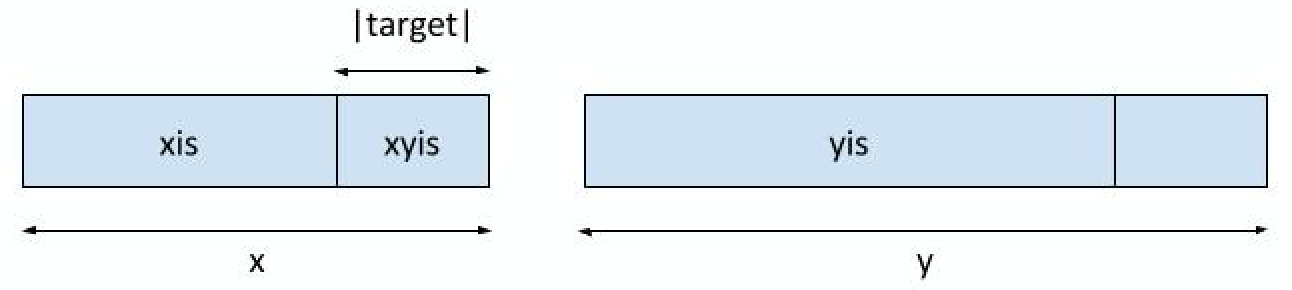
\includegraphics[scale=0.5]{text/stringmatcher/makeIndices}
\caption{Mappend indices of String Matcher.}
\label{fig:mappend:indices}
\end{figure}
%
The Haskell definition of @<>@, the monoid operation for @SM t@, is as follows.
\begin{code}
  (mappend)::forall (t::Symbol). KnownSymbol t => SM t -> SM t -> SM t
  (SM x xis) mappend (SM y yis)
    = SM (x stringMappend y) (xis' listMappend xyis listMappend yis')
    where
      tg   = fromString (symbolVal (Proxy :: Proxy t))
      xis' = map (castGoodIndexLeft tg x y) xis
      xyis = makeNewIndices x y tg
      yis' = map (shiftStringRight tg x y) yis
\end{code}
Note again that capturing target as a type parameter is critical,
otherwise there is no way for the Haskell's type system to specify
that both arguments of @(mappend)@ are string matchers on the same target.

The action of @(<>)@ on the two @input@ fields is straightforward;
however, the action on the two @indices@ is complicated by the need to
shift indices and the possibility of new matches arising from the
concatenation of the two @input@
fields. Figure~\ref{fig:mappend:indices} illustrates the three pieces
of the new @indices@ field which we now explain in more detail.

\mypara{1. Casting Good Indices}
If @xis@ is a list of good indices for the string @x@ and the target
@tg@, then @xis@ is also a list of good indices for the string
@x stringMappend y@ and the target @tg@, for each @y@.
%
To prove this property we need to invoke the property
@subStrAppendRight@ on Refined Strings that establishes
substring preservation on string right appending.
%
\begin{code}
  assume subStrAppendRight
      :: sl:RString -> sr:RString -> j:Int
      -> i:{Int | i + j <= lenStr sl }
      -> {subString sl i j = subString (sl stringMappend sr) i j}
\end{code}
%
The specification of @subStrAppendRight@ ensures that for each
string @sl@ and @sr@ and each integer @i@ and @j@ whose sum is within @sl@,
the substring from @i@ with length @j@ is identical in @sl@ and in @(sl stringMappend sr)@.
%
The function @castGoodIndexLeft@ applies the above property to an index @i@
to cast it from a good index on @sl@ to a good index on @(sl stringMappend sr)@
%
\begin{code}
  castGoodIndexLeft
    :: tg:RString -> sl:RString -> sr:RString
    -> i:GoodIndex sl tg
    -> {v:GoodIndex (sl stringMappend sr) target | v = i}

  castGoodIndexLeft tg sl sr i
    = cast (subStrAppendRight sl sr (lenStr tg) i) i
\end{code}
%
Where @cast p x@ returns @x@, after enforcing the properties of @p@ in the logic
\begin{code}
  cast :: b -> x:a -> {v:a | v = x}
  cast _ x = x
\end{code}
%
Moreover, in the logic, each expression @cast p x@
is reflected as @x@,
thus allowing random (\ie non-reflected) Haskell expressions to appear in @p@.

\mypara{2. Creation of new indices}
The concatenation of two input strings @sl@ and @sr@
may create new good indices.
%
For instance, concatenation of
@"ababcab"@ with @"cab"@
leads to a new occurence of @"abcab"@ at index @5@ which
does not occur in either of the two input strings.
%
These new good indices can appear only at the last @lenStr tg@ positions
of the left input @sl@.
%
@makeNewIndices sl sr tg@ detects all such good new indices.
%
\begin{code}
  makeNewIndices
    :: sl:RString -> sr:RString -> tg:RString
    -> [GoodIndex {sl stringMappend sr} tg]
    
  makeNewIndices sl sr tg
    | lenStr tg < 2 = []
    | otherwise     = makeIndices (sl stringMappend sr) tg lo hi
    where
      lo = maxInt (lenStr sl - (lenStr tg - 1)) 0
      hi = lenStr sl - 1
\end{code}
If the length of the @tg@ is less than 2, then no new good indices are created.
%
Otherwise,
the call on @makeIndices@ returns all the good indices of the input
@sl stringMappend sr@ for target @tg@
in the range from @maxInt (lenStr sl-(lenStr tg-1)) 0@ to  @lenStr sl-1@.
%

Generally, @makeIndices s tg lo hi@ returns the good indices
of the input string @s@ for target @tg@ in the range from @lo@ to @hi@.
%
\begin{code}
  makeIndices :: s:RString -> tg:RString -> lo:Nat
              -> hi:Int -> [GoodIndex s tg]
    
  makeIndices s tg lo hi  
    | hi < lo             = []
    | isGoodIndex s tg lo = lo:rest
    | otherwise           = rest
    where
      rest = makeIndices s tg (lo + 1) hi
\end{code}
%Note the similarity to the functional specification of string matching
%at the beginning of this section.

It is important to note that
@makeNewIndices@ does not scan all the input,
instead only searching at most @lenStr tg@ positions for new good indices.
%
Thus, the time complexity to create the new indices is linear
on the size of the target but independent of the size of the input.

\mypara{3. Shift Good Indices}
If @yis@ is a list of good indices on the string @y@ with target @tg@,
then we need to shift each element of @yis@ right @lenStr x@ units to
get a list of good indices for the string @x stringMappend y@.

%
To prove this property we need to invoke the property
@subStrAppendLeft@ on Refined Strings that establishes
substring shifting on string left appending.
%
\begin{code}
  assume subStrAppendLeft
    :: sl:RString -> sr:RString
    -> j:Int -> i:Int
    -> {subStr sr i j = subStr (sl stringMappend sr) (lenStr sl+i) j}
\end{code}
%
The specification of @subStrAppendLeft@ ensures that for each
string @sl@ and @sr@ and each integers @i@ and @j@,
the substring from @i@ with length @j@ on @sr@
is equal to the substring from @lenStr sl + i@
with length @j@ on @(sl stringMappend sr)@.
%
The function @shiftStringRight@ both shifts the input index @i@ by @lenStr sl@
and applies the @subStrAppendLeft@ property to it,
casting @i@ from a good index on @sr@ to a good index on @(sl stringMappend sr)@

Thus, @shiftStringRight@ both appropriately shifts the index
and casts the shifted index using the above theorem:
\begin{code}
  shiftStringRight
    :: tg:RString -> sl:RString -> sr:RString
    -> i:GoodIndex sr tg
    -> {v:(GoodIndex (sl stringMappend sr) tg) | v = i + lenStr sl}
    
  shiftStringRight tg sl sr i
    = subStrAppendLeft sl sr (lenStr tg) i `cast` i + lenStr sl
\end{code}

\subsubsection{String Matching is a Monoid}
Next we prove that the monoid methods @mempty@ and @(mappend)@ satisfy
the monoid laws.
%
\begin{theorem}[SM is a Monoid]\label{theorem:stringmatchers}
(@SM t@, @mempty@, @mappend@)
is a monoid.
\end{theorem}
%
\begin{proof}
According to the Monoid Definition~\ref{definition:monoid},
we prove that string matching is a monoid,
by providing safe implementations for the monoid law functions.
%
First, we prove \textit{left identity}.
\begin{code}
  idLeft :: x:SM t -> {mempty mappend x = xs}
  
  idLeft (SM i is)
    =   (mempty :: SM t) mappend (SM i is)
    =. (SM stringMempty listMempty) mappend (SM i is)
    =. SM (stringMempty <+> i) (is1 ++ isNew ++ is2)
       ? idLeftStr i
    =. SM i ([] ++ [] ++ is)
       ? (mapShiftZero tg i is && newIsNullRight i tg)
    =. SM i is
       ? idLeftList is
    ** QED
    where
      tg    = fromString (symbolVal (Proxy :: Proxy t))
      is1   = map (castGoodIndexRight tg i stringMempty) []
      isNew = makeNewIndices stringMempty i tg
      is2   = map (shiftStringRight tg stringMempty i) is
\end{code}

The proof proceeds by rewriting, using left identity of the monoid strings and lists,
and two more lemmata.
\begin{itemize}
\item Identity of shifting by an empty string.
\begin{code}
  mapShiftZero :: tg:RString -> i:RString
    -> is:[GoodIndex i target]
    -> {map (shiftStringRight tg stringMempty i) is = is}
\end{code}
The lemma is proven by induction on @is@ and
the assumption that empty strings have length 0.
\item No new indices are created.
\begin{code}
  newIsNullLeft :: s:RString -> t:RString 
                -> {makeNewIndices stringMempty s t = []}
\end{code}
The proof relies on the fact that @makeIndices@
is called on the empty range from @0@ to @-1@
and returns @[]@.
\end{itemize}

Next, we prove \textit{right identity}.
\begin{code}
  idRight :: x:SM t -> {x mappend mempty = x}
  
  idRight (SM i is)
    =  (SM i is) mappend (mempty :: SM t)
    =. (SM i is) mappend (SM stringMempty listMempty)
    =. SM (i stringMappend stringMempty) (is1 listMappend isNew listMappend is2)
       ? idRightStr i
    =. SM i (is listMappend N listMappend N)
       ? (mapCastId tg i stringMempty is && newIsNullLeft i tg)
    =. SM i is
       ? idRightList is
    **  QED
    where
      tg    = fromString (symbolVal (Proxy :: Proxy t))
      is1   = map (castGoodIndexRight tg i stringMempty) is
      isNew = makeNewIndices i stringEmp tg
      is2   = map (shiftStringRight tg i stringMempty) []
\end{code}
The proof proceeds by rewriting,
using right identity on strings and lists and two more lemmata.
\begin{itemize}
\item Identity of casting is proven
\begin{code}
  mapCastId 
    :: tg:RString -> x:RString -> y:RString
    -> is:[GoodIndex x tg] ->
    -> {map (castGoodIndexRight tg x y) is = is}
\end{code}
We prove identity of casts by induction on @is@ and
identity of casting on a single index.
\item No new indices are created.
\begin{code}
  newIsNullLeft 
    :: s:RString -> t:RString
    -> {makeNewIndices s stringMempty t = listMempty}
\end{code}
The proof proceeds by case splitting
on the relative length of @s@ and @t@.
At each case we prove by induction that all
the potential new indices would be out of bounds and thus
no new good indices would be created.
\end{itemize}

- Finally we prove \textit{associativity}.
For space, we only provide a proof sketch.
The whole proof is available online~\cite{implementation}.
%
Our goal is to show equality of the left and right associative string matchers.
%
\begin{code}
  assoc :: x:SM t -> y:SM t -> z:SM t
        -> {x mappend (y mappend z) = (x mappend y) mappend z}
\end{code}
To prove equality of the two string matchers we show
that the input and indices fields are respectively equal.
%
Equality of the input fields follows by associativity of RStrings.
%
Equality of the index list proceeds in three steps.
%
\begin{enumerate}
\item Using list associativity and distribution of index shifting,
we group the indices in the five lists shown in
Figure~\ref{fig:mappend:assoc}: the indices of the input @x@, the new
indices from mappending @x@ to @y@, the indices of the input @y@, the
new indices from mappending @x@ to @y@, and the indices of the input
@z@.
\item The representation of each group depends on the order of appending.
For example, if @zis1@ (resp. @zis2@) is the group @zis@ when
right (resp. left) mappend happened first, then we have
\begin{code}
  zis1 = map (shiftStringRight tg xi (yi stringMappend zi))
             (map (shiftStringRight tg yi zi) zis)

  zis2 = map (shiftStringRight tg (xi stringMappend yi) zi) zis
\end{code}
That is, in right first, the indices of @z@ are first shifted
by the length of @yi@ and then by the length of @xi@,
while in the left first case, the indices of @z@ are shifted by the
length of @xi stringMappend yi@.
In this second step of the proof we prove, using lemmata,
the equivalence of the different group representations.
%
The most interesting lemma we use is called @assocNewIndices@ and proves
equivalence of all the three middle groups together
by case analysis on the relative lengths of the target @tg@ and the middle string @yi@.
\item After proving equivalence of representations,
we again use list associativity and distribution of casts to wrap the
index groups back in string matchers.
\end{enumerate}
\begin{figure}
\centering
\captionsetup{justification=centering}
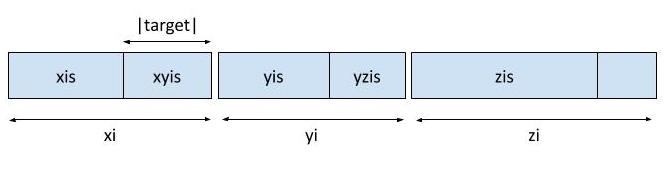
\includegraphics[scale=0.5]{text/stringmatcher/AssociativeIndices}
\caption{Associativity of String Matching.}
\label{fig:mappend:assoc}
\end{figure}
We now sketch the three proof steps, while the whole proof
is available online~\cite{implementation}.
\begin{code}
  assoc x@(SM xi xis) y@(SM yi yis) z@(SM zi zis)
    -- Step 1: unwrapping the indices
    =   x <> (y <> z)
    =. (SM xi xis) <> ((SM yi yis) <> (SM zi zis))
                         ...
    -- via list associativity and distribution of shifts
    =. SM i (xis1 ++ ((xyis1 ++ yis1 ++ yzis1) ++ zis1))
    -- Step 2: Equivalence of representations
    =. SM i (xis2 ++ ((xyis1 ++ yis1 ++ yzis1) ++ zis1))
       ? castConcat tg xi yi zi xis
    =. SM i (xis2 ++ ((xyis1 ++ yis1 ++ yzis1) ++ zis2))
       ? mapLenFusion tg xi yi zi zis
    =. SM i (xis2 ++ ((xyis2 ++ yis2 ++ yzis2) ++ zis2))
       ? assocNewIndices y tg xi yi zi yis
    -- Step 3: Wrapping the indices
                         ...
    -- via list associativity and distribution of casts
    =. (SM xi xis <> SM yi yis) <> SM zi zis
    =. (x <> y) <> z
    ** QED
    where
      i     = xi stringMappend (yi stringMappend zi)

      yzis1 = map (shiftStringRight tg xi (yi <+> zi)) yzis
      yzis2 = makeNewIndices (xi <+> yi) zi tg
      yzis  = makeNewIndices yi zi tg
      ...
\end{code}
\cqed\end{proof}


\subsection{String Matching Monoid Morphism}\label{subsec:smmorphism}
Next, we define the function @toSM :: RString -> SM target@ which does
the actual string matching computation for a set
target~\footnote{\texttt{toSM} assumes the target is clear from the
  calling context; it is also possible to write a wrapper function
  taking an explicit target which gets existentially reflected into
  the type.}
%
\ignore{ The function @toSM input@ creates a string matcher @SM
  target@ structure that matches the type level symbol target to the
  string value argument @input@.  }
%
\begin{code}
toSM :: forall (target :: Symbol). (KnownSymbol target)
     => RString -> SM target
toSM input = SM input (makeSMIndices input tg) where
  tg = fromString (symbolVal (Proxy :: Proxy target))

makeSMIndices
  :: x:RString -> tg:RString -> [GoodIndex x tg]
makeSMIndices x tg
  = makeIndices x tg 0 (lenStr tg - 1)
\end{code}
%
The input field of the result is the input string;
the indices field is computed by calling @makeIndices@
within the range of the @input@, that is from
@0@ to @lenStr input - 1@.
%
\begin{code}
\end{code}

We now prove that @toSM@ is a monoid morphism.
%
\begin{theorem}[$\texttt{toSM}$ is a Morphism]\label{theorem:smmorphism}
@toSM :: RString -> SM t@ is a morphism between the monoids
(@RString@, @stringMempty@, @stringMappend@) and (@SM t@, @mempty@, @mappend@).
\end{theorem}
\begin{proof}
Based on definition~\ref{definition:morphism}, proving @toSM@
is a morphism requires constructing a valid inhabitant of the type
\begin{code}
Morphism RString (SM t) toSM
  = x:RString -> y:RString
  -> {toSM stringMempty = mempty && toSM (x <+> y) = toSM x <> toSM y}
\end{code}
%
We define the function @distributestoSM :: Morphism RString (SM t) toSM@
to be the required valid inhabitant.

The core of the proof starts from
exploring the string matcher @toSM x <> toSM y@.
%
This string matcher contains three sets of indices
as illustrated in Figure~\ref{fig:mappend:indices}:
(1) @xis@ from the input @x@,
(2) @xyis@ from appending the two strings, and
(3) @yis@ from the input @y@.
%
We prove that appending these three groups of indices together gives
exactly the good indices of @x stringMappend y@, which are also the
value of the indices field in the result of
%
@toSM (x stringMappend y)@.
\begin{code}
distributestoSM x y
  =   (toSM x :: SM target) <> (toSM y :: SM target)
  ==. (SM x is1) <> (SM y is2)
  ==. SM i (xis ++ xyis ++ yis)
  ==. SM i (makeIndices i tg 0 hi1 ++ yis)
      ? (mapCastId tg x y is1 && mergeNewIndices tg x y)
  ==. SM i (makeIndices i tg 0       hi1
         ++ makeIndices i tg (hi1+1) hi)
      ? shiftIndicesRight 0 hi2 x y tg
  ==. SM i is
      ? mergeIndices i tg 0 hi1 hi
  ==. toSM (x <+> y)
  *** QED
  where
    xis  = map (castGoodIndexRight tg x y) is1
    xyis = makeNewIndices x y tg
    yis  = map (shiftStringRight   tg x y) is2
    tg   = fromString (symbolVal (Proxy::Proxy target))
    is1  = makeSMIndices x tg
    is2  = makeSMIndices y tg
    is   = makeSMIndices i tg
    i    = x <+> y
    hi1  = lenStr x - 1
    hi2  = lenStr y - 1
    hi   = lenStr i - 1
\end{code}
%
The most interesting lemma we use is
@mergeIndices x tg lo mid hi@
that states that for the input @x@ and the target @tg@
if we append the indices in the range  from @to@ to @mid@
with the indices in the range from @mid+1@ to @hi@,
we get exactly the indices in the range from @lo@ to @hi@.
%
This property is formalized in the type of the lemma.
\begin{code}
mergeIndices
 :: x:RString -> tg:RString
  -> lo:Nat -> mid:{Int | lo <= mid} -> hi:{Int | mid <= hi}
  -> {   makeIndices x tg lo hi
     =  makeIndices x tg lo mid
     ++ makeIndices x tg (mid+1) hi}
\end{code}
%
The proof proceeds by induction on @mid@ and using three more lemmata:
\begin{itemize}
\item @mergeNewIndices@ states that appending the indices @xis@ and @xyis@
is equivalent to the good indices of @x stringMappend y@ from @0@ to @lenStr x - 1@.
%
The proof case splits on the relative sizes of @tg@ and @x@
and is using @mergeIndices@ on @mid = lenStr x1 - lenStr tg@
in the case where @tg@ is smaller than @x@.
%
\item @mapCastId@ states that casting a list of indices returns the same list.
\item @shiftIndicesRight@ states that shifting right @i@ units the indices from @lo@ to @hi@
is equivalent to computing the indices from @i + lo@
to @i + hi@ on the string @x stringMappend y@, with @lenStr x = i@.
\end{itemize}
%%\begin{code}
%%mergeNewIndices
%%  :: tg:RString -> x:RString -> y:RString
%%  -> { makeSMIndices x tg
%%    ++ makeNewIndices x y tg
%%    == makeIndices (x <+> y) tg 0 (lenStr x - 1)}
%%\end{code}
%%The theorem states that appending the indices that appear in the first string @x@,
%%that is the indices @xis@ that do not and the indices @xyis@ that do involve @y@,
%%is equivalent to the indices @is@ on the input @x stringMappend y@
%%in the range from @0@ to @lenStr x -1@.
%%%
%%The proof case splits on the sizes of @tg@ and @x@.
%%%
%%If the size of the target is less than two, then @xyis@ is empty,
%%but @xis == is@, as appending @y@ to the input cannot create more indices.
%%%
%%Otherwise, if the input @x@ is smaller than the target,
%%then @xis@ is empty and @xyis@ is equal to @is@.
%%%
%%Otherwise, we set
%%and use the previous @mergeIndices@ lemma to merge @xis@ and @yis@ into @is@.
%%\item Shifting is left concatenation.
%%\begin{code}
%%shiftIndicesRight
%%  :: lo:Nat -> hi:Int
%%  -> x:RString -> y:RString
%%  -> tg:RString
%%  -> { map (shiftStringRight tg x y)
%%           (makeIndices y tg lo hi)
%%  == makeIndices (x stringMappend y) tg
%%                 (lenStr x + lo) (lenStr x + hi) }
%%
%%\end{code}
%%The lemma states that shifting indices from @lo@ to @hi@ on @y@
%%is equivalent to computing the indices from @lenStr x + lo@
%%to @lenStr x + hi@ on @x stringMappend y@,
%%and it is proved by induction on the difference @hi - lo@.
%%\end{itemize}
\qed\end{proof}


\subsection{Parallel String Matching}\label{subsec:parallel-string-matching}
We conclude this section with
the definition of a parallelized version of string matching.
%
We put all the theorems together to prove 
that the sequential and parallel versions always give the same result.
% and compare their time complexities.

We define @toSMPar@ as a parallel version of @toSM@ using machinery of section~\ref{sec:parallelization}.
\begin{code}
toSMPar :: forall (target :: Symbol). (KnownSymbol target)
        => Int -> Int -> RString -> SM target
toSMPar i j = pmconcat i . pmap toSM . chunkStr j
\end{code}
%
First, @chunkStr@ splits the input into @j@ chunks.
%
Then, @pmap@ applies @toSM@ at each chunk in parallel.
Finally, @pmconat@ concatenates the mapped chunks in parallel
using @mappend@, the monoidal operation for @SM target@.

\paragraph{Correctness.}
We prove correctness of @toSMPar@ directly from
Theorem~\ref{theorem:two-level}.
\begin{theorem}[Correctness of Parallel String Matching]\label{theorem:correctness}
For each parameter @i@ and @j@, and input @x@,
@toSMPar i j x@ is always equal to @toSM x@.
\begin{code}
correctness :: i:Int -> j:Int -> x:RString
             -> {toSM x = toSMPar i j x}
\end{code}
\end{theorem}

\begin{proof}
The proof follows by direct application of Theorem~\ref{theorem:two-level}
on the chunkable monoid (@RString@, @$\eta$@, @<+>@) (by Assumption~\ref{assumption:rstring})
and the monoid (@SM t@, @$\epsilon$@, @<>@) (by Theorem~\ref{theorem:stringmatchers}).
%
\begin{code}
correctness i j x
  =   toSMPar i j x
  ==. pmconcat i (pmap toSM (chunkStr j x))
  ==. toSM is
    ? parallelismEquivalence toSM distributestoSM x i j
  *** QED
\end{code}
%
Note that application of the theorem @parallelismEquivalence@
requires a proof that its first argument @toSM@ is a morphism.
%
By Theorem~\ref{theorem:monoid:distribution},
the required proof is provided as the function @distributestoSM@.
\qed\end{proof}

\ignore{

\paragraph{Time Complexity.}
Counting only string comparisons as the expensive operations,
the sequential string matcher on input @x@ runs in time
linear to @n = lenStr x@. Thus $T_\texttt{toSM}(n) = O(n)$.

We get time complexity of @toSMPar@ by the time complexity of
two-level parallel algorithms equation~\ref{eq:complexity},
with the time of string matching mappend being linear on the length
of the target @t = lenStr tg@, or
$T_\mappend(\texttt{SM})= O(t)$.
%
$$
T_\texttt{toSMPar} (n, t, i, j) =
O((i-1)(\frac{\log n - \log j}{\log i}) t  + \frac{n}{j})
$$
%
The above analysis refers to a model with infinite processor and no caching.
To compare the algorithms in practice,
we matched the target "the"
in  Oscar Wilde's "The Picture of Dorian Gray", a text of @n = 431372@ characters
using a two processor Intel Core i5.
%
The sequential algorithm detected 4590 indices in 40 ms.
%
We experimented with different parallization factors @i@ and chunk sizes @j / n@
and observed up to $50\%$ speedups of the parallel algorithm for parallelization factor
@4@ and @8@ chunks.
%
As a different experiment, we matched the input against its size @t = 400@ prefix,
a size comparable to the input size @n@.
%
For bigger targets,
mappend gets slower, as it has complexity linear to the size of target.
%
We observed $20\%$ speedups for @t=400@ target but also $30\%$ slow downs for various sizes of @i@ and @j@.
%
In all cases the indices returned by the sequential and the parallel algorithms were the same.
}


\section{Evaluation: Strengths \& Limitations}\label{sec:evaluation}

Verification of Parallel String Matching is the first realistic
proof that uses (Liquid) Haskell
to prove properties \textit{about} program functions.
%
In this section we use the String Matching proof
to quantitatively and qualitatively evaluate theorem proving in Haskell.

\paragraph{Quantitative Evaluation.}
The Correctness of Parallel String Matching proof
can be found online~\cite{implementation}.
%
Verification time, that is the time Liquid Haskell needs to check the proof,
is 75 sec on a dual-core Intel Core i5-4278U processor.
%
The proof consists of \textit{1839} lines of code.
%
Out of those
\begin{itemize}
\item \textit{226} are Haskell ``runtime'' code,
\item \textit{112} are liquid comments on the ``runtime'' Haskell code,
\item \textit{1307} are Haskell proof terms, that is functions with @Proof@ result type, and
\item \textit{194}  are liquid comments to specify theorems.
\end{itemize}
Counting both liquid comments and Haskell proof terms as verification code,
we conclude that the proof requires 7x the lines of ``runtime'' code.
%
This ratio is high and takes us to 2006 Coq,
when Leroy~\cite{Leroy06formalcertification} verified
the initial CompCert C compiler with
the ratio of verification to compiler lines being 6x.
% 4,400 lines of compiler code and 28,000 lines devoted to verification.

\paragraph{Strengths.}
Though currently verbose,
deep verification using Liquid Haskell has many benefits.
%
First and foremost,
\textit{the target code is written in the general purpose Haskell}
and thus can use advanced Haskell features, including
type literals, deriving instances, inline annotations
and optimized library functions like @ByteString@.
Even diverging functions can coexist with the target code, as long
as they are not reflected into logic~\cite{Vazou14}.

Moreover, \textit{SMTs are used to automate the proofs}
over key theories like linear arithmetic and equality.
%
As an example, associativity of @(+)@
is assumed throughout the proofs while shifting indices.
%
Our proof could be further automated 
by mapping refined strings to SMT strings and  
using the automated SMT string theory.
%
We did not follow this approach because we want to show that
our techinique can be used to prove any (and not only domain specific)
program properties.

Finally, we get further automation via
\textit{Liquid Type Inference}~\cite{LiquidPLDI08}.
%
Properties about program functions,
expressed as type specifications with unit result,
often depend on program invariants,
expressed as vanilla refinement types, and vice versa.
%
For example, we need the invariant that all indices of
a string matcher are good indices
to prove associativity of @(mappend)@.
%%NV simplify the above.
%%%For example, we need the invariant that all indices of
%%%a string matcher are good indices
%%%to prove that
%%%when the target is smaller than the input
%%%then the indices field is an empty list,
%%%which is required to prove associativity of @(mappend)@
%
Even though Liquid Haskell cannot currently synthesize proof terms,
it performs really well at inferring and propagating program invariants (like good indices)
via the abstract interpretation framework of Liquid Types.

\paragraph{Limitations.}
There are severe limitations that should be addressed
to make theorem proving in Haskell a pleasant and usable technique.
%
As mentioned earlier \textit{the proofs are verbose}.
%
There are a few cases where the proofs require domain specific knowledge.
%
For example, to prove associativity of string matching
@x mappend (y mappend z) = (x mappend y) mappend z@
we need a theorem that performs case analysis on the relative length of
the input field of @y@ and the target string.
%
Unlike this case split though, most proofs
do not require domain specific knowledge and merely proceed
by term rewriting and structural inductuction
that should be automated
via Coq-like~\cite{coq-book} tactics or/and Dafny-like~\cite{dafny} heuristics.
%
For example, synquid~\cite{polikarpova16} could be used to automatically
synthesize proof terms.

Currently, we suffer from two engineering limitations.
%
First, all reflected function should exist in the same module,
as reflection needs access to the function implementation
that is unknown for imported functions.
%
This is the reason why we need to use a user defined,
instead of Haskell's built-in, list.
%
In our implementation we used @CPP@ as a current workaround
of the one module restriction.
%
Second, class methods
cannot be currently reflected.
%
Our current workaround is to define Haskell functions instead
of class instances.
For example (@append@, @nil@) and (@concatStr@, @emptyStr@)
define the monoid methods of List and Refined String respectively.

Overall, we believe that the strengths outweigh the limitations which
will be addressed in the near future,
rendering Haskell a powerful theorem prover.



\chapter{Related Work}\label{chapter:related}

\section{Refinement Types in Practice}\label{sec:realword:related}

Next, we situate \toolname with 
existing Haskell verifiers.

\spara{Dependent Types} are the basis of many verifiers, 
or more generally, proof assistants.
%
Verification of haskell code is possible with
``full'' dependently typed systems like Coq~\cite{coq-book}, 
Agda~\cite{norell07}, Idris~\cite{Brady13}, Omega~\cite{Sheard06}, and
 {$\lambda_\rightarrow$}~\cite{LohMS10}.
 %
 While these systems are highly expressive,
their expressiveness comes at the cost of making logical validity checking undecidable
thus rendering verification cumbersome.	
 %
 Haskell itself can be considered a dependently-typed language,
 as type level computation is allowed via 
 Type Families~\cite{McBride02},
 Singleton Types\cite{Weirich12}, 
 Generalized Algebraic  Datatypes (GADTs)~\cite{JonesVWW06, SchrijversJSV09}, 
 and type-level functions~\cite{ChakravartyKJ05}.
 %
Again, 
verification in haskell itself turns out to be quite painful~\cite{LindleyM13}.

\spara{Refinement Types} are a form of dependent types where 
invariants are encoded via a combination of types and predicates
from a restricted \emph{SMT-decidable} 
logic~\cite{Rushby98,pfenningxi98,Dunfield07,GordonTOPLAS2011}. 
%
\toolname uses Liquid Types~\cite{LiquidPLDI09} 
that restrict the invariants even more
to allow type inference, a crucial feature of a usable type system.
%
Even though the language of refinements is restricted,
as we presented, the combination of
Abstract Refinements~\cite{vazou13} 
with sophisticated measure definitions 
allows specification and verification of a wide variety 
of program properties.

\spara{Static Contract Checkers} 
like ESCJava~\cite{ESCJava} are a classical way of verifying 
correctness through assertions and pre- and post-conditions. 
%
\cite{XuPOPL09} describes a static contract checker for 
Haskell that uses symbolic execution to unroll procedures
upto some fixed depth, yielding weaker ``bounded'' soundness
guarantees.
% 

Similarly, Zeno~\cite{ZENO} is an automatic Haskell 
prover that combines unrolling with heuristics for rewriting
and proof-search. 
%%Based on rewriting, it is sound but 
%%``Zeno might loop forever'' when faced with 
%%non-termination.
%
Finally, the Halo~\cite{halo} contract checker encodes 
Haskell programs into first-order logic by directly 
modeling the code's denotational semantics,
again, requiring heuristics for instantiating axioms 
describing functions' behavior.
%


\spara{Totality Checking}
is feasible by GHC itself, via an option flag that warns of any incomplete patterns.
%
Regrettably, GHC's warnings are local, \ie
GHC will raise a warning for @head@'s partial definition, 
but not for its caller, as the programmer would desire.
%%(2)~ and preservative:
%%a warning will be raised for any incomplete pattern
%%without an attempt to reason if it is reachable or not.
%
Catch~\cite{catch}, 
a fully automated tool that tracks incomplete patterns,
addresses the above issue
%
by computing functions' pre- and post-conditions.
Moreover, catch statically analyses the code 
to track reachable incomplete patterns.
%
\toolname allows more precise analysis than catch, 
thus, by assigning the appropriate
types to $\star$Error functions (\S~\ref{sec:totality}) 
it tracks reachable incomplete patters 
%we get catch analysis
as a side-effect of verification.

\spara{Termination Analysis}
is crucial for \toolname's soundness 
and is implemented in a technique inspired by~\cite{XiTerminationLICS01}, 
%
Various other authors have proposed techniques to verify termination of
recursive functions, either using the ``size-change
principle''~\cite{JonesB04,Sereni05}, or by annotating types with size indices
and verifying that the arguments of recursive calls have smaller
indices~\cite{HughesParetoSabry96,BartheTermination}.
%
To our knowledge, none of the above analyses have been empirically
evaluated on large and complex real-world libraries.

AProVE~\cite{Giesl11} implements a powerful, fully-automatic
termination analysis for Haskell based on term-rewriting.
%
Compared to AProVE,
encoding the termination proof via 
refinements provides advantages that are crucial in 
large, real-world code bases. 
Specifically, refinements
let us
%
(1) prove termination over a subset 
    (not all) of inputs; many functions (\eg @fac@) 
    terminate only on @Nat@ inputs and not all @Int@s,
%
(2) encode pre-conditions, 
    post-conditions, and auxiliary invariants that 
    are essential for proving termination, (\eg @qsort@),
%
(3) easily specify non-standard 
    decreasing metrics and prove termination, (\eg @range@).
%
In each case, the code could be (significantly) 
\emph{rewritten} to be amenable to AProVE but this defeats
the purpose of an automatic checker.
%


\section{Refinement Types for Haskell}\label{sec:refinedhaskell:related}

Next we situate our work with closely related lines of research.

\spara{Dependent Types} are the basis of many verifiers, 
or more generally, proof assistants.
%
In this setting arbitrary terms may appear inside types,
so to prevent logical inconsistencies, and enable
the checking of type equivalence, all terms must
terminate.
%
``Full'' dependently typed systems like Coq~\cite{coq-book}, 
Agda~\cite{norell07}, and Idris~\cite{Brady13} typically use 
\emph{structural} checks where recursion is allowed on 
sub-terms of ADTs to ensure that \emph{all} terms terminate.
%
We differ in that, since the refinement logic is
restricted, we do not require that all functions terminate,
and hence, we can prove properties of possibly diverging 
functions like @collatz@ as well as lazy functions like @repeat@.
%
Recent languages like Aura~\citep{AURA} and Zombie~\citep{Zombie}
allow general recursion, but constrain the logic to a terminating 
sublanguage, as we do, to avoid reasoning 
about divergence in the logic.
%
In contrast to us, the above systems crucially assume 
\emph{call-by-value} semantics to ensure that binders are bound
to values, \ie cannot diverge.





   Haskell itself can be used to \emph{fake} ``lightweight'' dependent 
   types~\citep{ChakravartyKJ05,JonesVWW06,Weirich12}.
   In this style, the invariants are expressed in 
   a restricted~\citep{Jia10} total 
   index language and relationships (\eg $x<y$ and $y<z$) 
   are combined (\eg $x<z$) by explicitly constructing
   a term denoting the consequent from terms 
   denoting the antecedents.
   %
   On the plus side this ``constructive'' approach
   ensures soundness. 
   It is impossible to witness inconsistencies, 
   as doing so triggers diverging computations.
   %
   However, it is not easy to use restricted indices
   with explicitly constructed relations to verify 
   complex properties~\citep{hasochism}.


\spara{Refinement Types} are a form of dependent types where 
invariants are encoded via a combination of types and predicates
from a restricted \emph{SMT-decidable} 
logic~\cite{Rushby98,pfenningxi98,Dunfield07,GordonTOPLAS2011}. 
%
The restriction makes it safe to support arbitrary recursion, 
which has hitherto never been a problem for refinement types.
%
However, we show that this is because all the above systems 
implicitly assume that all free variables are bound to values, 
which is only guaranteed under CBV and, as we have seen, leads 
to unsoundness under lazy evaluation.



\spara{Tracking Divergent Computations}
The notion of type stratification to track potentially 
diverging computations dates to at least~\citep{ConstableS87} 
which uses $\bar{\typ}$ to encode diverging terms, and types 
$\efix{}$ as $(\bar{\typ}\rightarrow\bar{\typ}) \rightarrow \bar{\typ}$).
%
More recently, \cite{Capretta05} tracks diverging 
computations within a \emph{partiality monad}.
%
Unlike the above, we use refinements to 
obtain terminating fixpoints (\etfix{}), which let us prove 
the vast majority (of sub-expressions) in real world libraries 
as non-diverging, avoiding the restructuring that would
be required by the partiality monad.

\spara{Termination Analyses}
Various authors have proposed techniques to verify termination 
of recursive functions, either using the ``size-change principle'' 
\cite{JonesB04,Sereni05}, or by annotating types with size indices 
and verifying that the arguments of recursive calls have smaller 
indices~\cite{HughesParetoSabry96,BartheTermination}.
%
Our use of refinements to encode terminating fixpoints is most 
closely related to~\cite{XiTerminationLICS01}, but this work 
also crucially assumes CBV semantics for soundness.

AProVE~\cite{Giesl11} implements a powerful, fully-automatic
termination analysis for Haskell based on term-rewriting.
%
While we could use an external analysis like AProVE,
we have found that encoding the termination proof via 
refinements provided advantages that are crucial in 
large, real-world code bases. Specifically, refinements
let us
%
(1) prove termination over a subset 
    (not all) of inputs; many functions (\eg @fac@) 
    terminate only on @Nat@ inputs and not all @Int@s,
%
(2) encode pre-conditions, 
    post-conditions, and auxiliary invariants that 
    are essential for proving termination, (\eg @gcd@),
%
(3) easily specify non-standard 
    decreasing metrics and prove termination, (\eg @range@).
%
In each case, the code could be (significantly) 
\emph{rewritten} to be amenable to AProVE but this defeats
the purpose of an automatic checker.
%
Finally, none of the above analyses have been empirically
evaluated on large and complex real-world libraries.


\spara{Static Contract Checkers} 
like ESCJava~\cite{ESCJava} are a classical way of verifying 
correctness through assertions and pre- and post-conditions. 
%
Side-effects like modifications of global variables are a 
well known issue for static checkers for imperative languages;
the standard approach is to use an effect analysis to determine
the ``modifies clause'' \ie the set of globals modified by a procedure.
%
Similarly, one can view our approach as implicitly computing 
the non-termination effects.
%
%
\cite{XuPOPL09} describes a static contract checker for 
Haskell that uses symbolic execution to unroll procedures
upto some fixed depth, yielding weaker ``bounded'' soundness
guarantees.
% 

%
Similarly, Zeno~\cite{ZENO} is an automatic Haskell 
prover that combines unrolling with heuristics for rewriting
and proof-search. 
Based on rewriting, it is sound but 
``Zeno might loop forever'' when faced with 
non-termination.
%
Finally, the Halo~\cite{halo} contract checker encodes 
Haskell programs into first-order logic by directly 
modeling the code's denotational semantics,
again, requiring heuristics for instantiating axioms 
describing functions' behavior. Halo's translation of Haskell
programs directly encodes constructors as uninterpreted functions,
axiomatized to be injective (as the denotational semantics requires).
This heavyweight encoding is more precise than predicate abstraction 
but leads to model-theoretic problems (outlined in the Halo paper) and 
affects the efficiency of the encoding when scaling to larger programs 
(see also \ref{sec:refinedhaskell:conclusion}, paragraph B) in the lack of specialized 
decisions procedures.
%
Unlike any of the above, our type-based approach does 
not rely on heuristics for unrolling recursive procedures, 
or instantiating axioms. 
%
Instead we are based on decidable SMT validity 
checking and abstract interpretation~\cite{LiquidPLDI08} 
which makes the tool predictable and the overall workflow
scale to the verification of large, real-world
code bases.

\section{Abstract Refinement Types}\label{sec:related}

The notion of type refinements was introduced by Freeman and
Pfenning~\cite{FreemanPfenning91}, with refinements limited to
restrictions on the structure of algebraic datatypes, for which
inference is decidable.
%
Our present notion of refinement types has its roots in the
\emph{indexed types} of Xi and Pfenning~\cite{pfenningxi98}, wherein
data types' ranges are restricted by \emph{indices}, analogous to our
refinement predicates, drawn from a decidable domain; in the example
case explored by Xi and Pfenning, types were indexed by terms from
Presburger arithmetic.
%
Since then, several approaches to developing richer refinement type
systems and accompanying methods for type checking have been
developed.
%
Knowles and Flanagan~\cite{Knowles10} allow refinement predicates to
be arbitrary terms of the language being typechecked and present a
technique for deciding some typing obligations statically and
deferring others to runtime.
%; Gronksi \etal~\cite{Gronski06} present animplementation of such a system.
%
Findler and Felleisen's~\cite{Findler02} higher-order contracts, which
extend Eiffel's~\cite{MeyerBook} first-order contracts --- ordinary
program predicates acting as dynamic pre- and post-conditions --- to
the setting of higher-order programs, eschew any form of static
checking, and can be seen as a dynamically-checked refinement type
system.
%
Bengtson \etal~\cite{GordonTOPLAS2011} present a refinement type
system in which type refinements are drawn from a decidable logic,
making static type checking tractable.
%
Greenberg \etal~\cite{Greenberg11} gives a rigorous treatment of the
metatheoretic properties of such a refinement type system.

Refinement types have been applied to the verification of a variety of
program properties~\cite{pfenningxi98,Dunfield,GordonTOPLAS2011,FournetCCS11}.
%
In the most closely related work to our own, Kawaguchi \etal~\cite{LiquidPLDI09} 
introduce \emph{recursive} and \emph{polymorphic} refinements for data
structure properties.
%
The present work unifies and generalizes these two somewhat ad-hoc notions 
into a single, strictly and significantly more expressive mechanism of
abstract refinements.

%  Higher-order logics: Coq/HTT/F*/Agda which have explicit predicates, quantification 
A number of higher-order logics and corresponding verification tools
have been developed for reasoning about programs.
%
Example of systems of this type include NuPRL \cite{Constable86},
%F$_{<:}$ \cite{Cardelli91},
Coq \cite{coq-book}, F$^\star$ \cite{SwamyCFSBY11} and Agda \cite{norell07}
which support the development and verification of higher-order, 
pure functional programs.
%
While these systems are highly expressive, their expressiveness comes at the
cost of making logical validity checking undecidable.
%
To help automate validity checking, both built-in and user-provided
tactics are used to attempt to discharge proof obligations; however,
the user is ultimately responsible for manually proving any
obligations which the tactics are unable to discharge.

\section{Bounded Refinement Types}\label{sec:abstractrefinements:related}

\paragraph{Higher order Logics and Dependent Type Systems}
%
including
NuPRL~\citep{Constable86},
Coq~\citep{coq-book}, Agda~\citep{norell07},
and even to some extent, \haskell~\citep{JonesVWW06, McBride02},
occupy the maximal extreme of the expressiveness spectrum.
However, in these settings, checking requires explicit
proof terms which can add considerable programmer overhead.
%
Our goal is to eliminate the programmer overhead of
proof construction by restricting specifications to
decidable, first order logics and to see how far
we can go without giving up on expressiveness.
%
The \fstar system enables full dependent typing via
SMT solvers via a higher-order universally quantified
logic that permit specifications similar to ours
(\eg @compose@, @filter@ and @foldr@).
%% https://github.com/FStarLang/FStar/
%
While this approach is at least as expressive
as bounded refinements it has two drawbacks.
%
First, due to the quantifiers, the generated VCs
fall outside the SMT decidable theories.
This renders the type system undecidable (in theory),
forcing a dependency on the solver's unpredictable
quantifier instantiation heuristics (in practice).
%
Second, more importantly, % perhaps more importantly,
the higher order
predicates must be \emph{explicitly} instantiated,
placing a heavy annotation burden on the programmer.
%
In contrast, bounds permit decidable
checking, and are automatically instantiated
via Liquid Types.


\paragraph{Our notion of Refinement Types}
%
has its roots in the predicate subtyping
of PVS~\cite{Rushby98} and \emph{indexed types}
(DML~\cite{pfenningxi98}) where types are constrained
by predicates drawn from a logic.
%
To ensure decidable checking several refinement
type systems including~\citep{pfenningxi98,Dunfield07,LiquidICFP14}
restrict refinements to decidable, quantifier free logics.
%
While this ensures predictable checking and inference~\cite{LiquidPLDI08}
it severely limits the language of specifications, and makes it hard to
fashion simple higher order abstractions like @filter@ (let alone the more
complex ones like relational algebras and state transformers.)

\paragraph{To Reconcile Expressiveness and Decidability}
%
\catalyst~\citep{catalyst} permits a form of
higher order specifications where refinements
are relations which may themselves be parameterized
by other relations, which allows for example, a
way to precisely type @filter@ by suitably
composing relations.
%
However, to ensure decidable checking, \catalyst
is limited to relations that can be specified as
catamorphisms over inductive types, precluding
for example, theories like arithmetic.
More importantly, (like \fstar), \catalyst provides
no inference: higher order relations must be
\emph{explicitly} instantiated.
%
Bounded refinements build directly upon
abstract refinements~\citep{vazou13},
a form of refinement polymorphism
analogous to parametric polymorphism.
%
While \cite{vazou13} adds expressiveness via
abstract refinements, without bounds we cannot
specify any \emph{relationships between} the
abstract refinements. The addition of bounds
makes it possible to specify and verify the examples
shown in this paper,
while preserving decidability and inference.

\paragraph{Our Relational Algebra Library} builds on a long
line of work on type safe database access.
%
The HaskellDB~\citep{haskellDB}
showed how phantom types could be used to eliminate
certain classes of errors.
%
Haskell's HList library~\citep{heterogeneous}
extends this work with type-level computation
features to encode heterogeneous lists, which
can be used to encode database schema, and
(unlike HaskellDB) statically reject accesses
of ``missing'' fields.
%
The HList implementation is non-trivial,
requiring new type-classes for new operations
(\eg @append@ing lists); \citep{thepipower}
shows how a dependently typed language greatly
simplifies the implementation.
%
Much of this simplicity can be recovered in
Haskell using the @singleton@ library~\citep{Weirich12}.
%
Our goal is to show that bounded refinements
are expressive enough to permit the construction
of rich abstractions like a relational algebra
and generic combinators for safe database access
while using SMT solvers to provide decidable
checking and inference. Further, unlike the
HList based approaches, refinements they can
be used to \emph{retroactively} or \emph{gradually}
verify safety; if we erase the types we still
get a valid Haskell program operating over
homogeneous lists.


\paragraph{Our Approach for Verifying Stateful Computations} using monads
indexed by pre- and post-conditions is inspired by the method of
Filli\^atre~\citep{Filliatre98}, which was later enriched with
separation logic in Ynot~\citep{ynot}. In future work it would
be interesting to use separation logic based refinements to specify
and verify the complex sharing and aliasing patterns allowed by Ynot.
%
\fstar encodes stateful computations in a special Dijkstra
Monad~\citep{dijkstramonad} that replaces the two assertions with
a single (weakest-precondition) predicate transformer which
can be composed across sub-computations to yield a transformer
for the entire computation.
%
Our \RIO approach uses the idea of indexed monads but
has two concrete advantages.
%
First, we show how bounded refinements alone suffice to
let us fashion the \RIO abstraction from scratch.
%
Consequently, second, we automate inference of pre- and
post-conditions and loop invariants as refinement instantiation
via Liquid Typing~\citep{LiquidPLDI08}.


\section{Refinement Reflection}\label{sec:refinementreflection:related}

% We compare refinement reflection to the most closely related
% lines of work in the vast literature on program verification.

\mypara{SMT-Based Verification}
%
SMT-solvers have been extensively used to automate
program verification via Floyd-Hoare logics~\cite{Nelson81}.
%
Our work is inspired by Dafny's Verified
Calculations~\citep{LeinoPolikarpova16},
a framework for proving theorems in
Dafny~\citep{dafny}, but differs in
%
(1)~our use of reflection instead of axiomatization and
(2)~our use of refinements to compose proofs.
%
Dafny, and the related \fstar~\citep{fstar}
which like \toolname, uses types to compose
proofs, offer more automation by translating
recursive functions to SMT axioms.
However, unlike reflection, this axiomatic
approach renders typechecking and verification
undecidable (in theory) and leads to
unpredictability and divergence
(in practice)~\citep{Leino16}.
%\NV{CHECL Relational-F*, Barthe et al, from POPL 2014, and EasyCrypt}

%% In a work more closely related to
%% ours, \fstar uses refinement types
%% for program verification supporting
%% expressiveness of fully dependent types.
%% %
%% As in Dafny, \fstar directly translates
%% recursive functions to axioms in the logic
%% thus suffers from the ``butterfly effect''
%% and allows the user to explicitly write SMT tactics to control it.

%% Leino \etal~\citep{Leino16}
%% name this problem as the ``butterfly
%% effect'', in which minor modifications
%% to the program source cause significant
%% instabilities in verification and propose
%% trigger selection strategies to address it.
%% %
%% We avoid the ``butterfly effect'' by not
%% directly axiomatizing functions into logic.
%% Instead the information about the function's
%% body is exactly captured in function's result
%% type and user needs to explicitly invoke the function to push
%% the function's definition information into the logic.


\mypara{Dependent types}
%
Our work is also inspired by dependently typed
systems like Coq~\citep{coq-book} and
Agda~\citep{agda}.
%
Reflection shows how deep specification
and verification in the style of Coq and Agda
can be \emph{retrofitted} into existing languages
via refinement typing.
%
Furthermore, we can use SMT to significantly
automate reasoning over important theories like
arithmetic, equality and functions.
%
It would be interesting to investigate how
the tactics and sophisticated proof search
of Coq \etc can be adapted to the refinement setting.

% which allow for arbitrary expressiveness of the type system
% in the cost of automatic verification.
%
%% The syntax of \libname's operators is inspired by
%% Equational Reasoning in Agda~\citep{agda}.
%% Here we extended these equational operators
%% to support linear arithmetic and, for example, prove
%% properties of Ackermann function.
%% %
%% Unlike Adga, proof term are explicit in \libname,
%% we do not use heuristics to infer proofs.


\mypara{Dependent Types for Non-Terminating Programs}
%
Zombie~\citep{Zombie, Sjoberg2015} integrates
dependent types in non terminating programs
and supports automatic reasoning for equality.
%
Vazou \etal have previously~\citep{Vazou14} shown
how Liquid Types can be used to check
non-terminating programs.
%
Reflection makes \toolname at least as
expressive as Zombie, \emph{without}
having to axiomatize the theory of
equality within the type system.
%
Consequently, in contrast to Zombie,
SMT based reflection lets \toolname
verify higher-order specifications
like @foldr_fusion@.

% which lets us use SMT automation
% to verify deep specifications of
% non-trivial programs.
%
% Our current extension is orthogonal to the
% previous work: our system remains sound as
% long as logical terms provably terminate.
%
% We get automation from SMT solvers for not only
% the theory of equality, but also linear arithmetic.
%
% \NV{Zombie with rewritting does not allow HIGHER ORDER reasoning}

\mypara{Dependent Types in Haskell}
%
Integration of dependent types into Haskell
has been a long standing goal that dates back
to Cayenne~\citep{cayenne}, a Haskell-like,
fully dependent type language with undecidable
type checking.
%
In a recent line of work~\citep{EisenbergS14}
Eisenberg \etal aim to allow fully dependent
programming within Haskell, by making
``type-level programming ... at least as
  expressive as term-level programming''.
%
Our approach differs in two significant ways.
%
First, reflection allows SMT-aided verification,
which drastically simplifies proofs over key theories
like linear arithmetic and equality.
%
Second, refinements are completely erased at run-time.
That is, while both systems automatically lift Haskell
code to either uninterpreted logical functions
or type families, with refinements, the logical
functions are not accessible at run-time and
promotion cannot affect the semantics of
the program.
%
As an advantage (resp. disadvantage), refinements
cannot degrade (resp. optimize)
the performance of programs.

\mypara{Proving Equational Properties}
% of Haskell Programs}
%
Several authors have proposed tools for proving
(equational) properties of (functional) programs.
%
Systems~\citep{sousa16} and \citep{KobayashiRelational15}
extend classical safety verification algorithms,
respectively based on Floyd-Hoare logic and Refinement Types,
to the setting of relational or $k$-safety properties
that are assertions over $k$-traces of a program.
%
Thus, these methods can automatically prove that
certain functions are associative, commutative \etc.
but are restricted to first-order properties and
are not programmer-extensible.
%
Zeno~\citep{ZENO} generates proofs by term
rewriting and Halo~\citep{halo} uses an axiomatic
encoding to verify contracts.
%
Both the above are automatic, but unpredictable and not
programmer-extensible, hence, have been limited to
far simpler properties than the ones checked here.
%
HERMIT~\citep{Farmer15} proves equalities by rewriting
the GHC core language, guided by user specified scripts.
%
In contrast, our proofs are simply Haskell programs,
we can use SMT solvers to automate reasoning, and,
most importantly, we can connect the validity of
proofs with the semantics of the programs.

% \RJ{say: hermit does typeclass laws}
%
% \NV{TO ADD Naoki and class laws for TFP}
%
%% Compared to these systems, our proofs are
%% expressed as Haskell programs and do not
%% require the user to learn a different
%% tactic languages.
%% %
%% Moreover, our system is more general
%% as it allows for both equational
%% and linear arithmetic proofs.
%% %
%% On the other hand, \libname requires
%% explicit proofs and does not currently
%% support any automatic heuristics.

\mypara{Deterministic Parallelism}
%
Deterministic parallelism has plenty of theory but relatively few practical
implementations.  Early discoveries were based on limited producer-consumer
communication, such as single-assignment variables \cite{Tesler-1968,IStructures}, Kahn
process networks~\cite{kahn-1974}, and synchronous dataflow~\cite{lee-sdf}.
Other models use synchronous updates to shared state, as in
Esterel~\cite{synchronous-overview} or PRAM.  Finally, work on type systems for
permissions management \cite{permission-types,habanero-java-permissions},
supports the development of {\em non-interfering} parallel programs that access
disjoint subsets of the heap in parallel.  Parallel functional programming is
also non-interfering~\cite{manticore,multicore-ghc}.
%
Irrespective of which theory is used to support deterministic parallel
programming, practical implementations such as Cilk~\cite{cilk} or Intel
CnC~\cite{cnc} are limited by host languages with type systems insufficient to
limit side effects, much less prove associativity.  Conversely, dependently
typed languages like Agda and Idris do not have parallel programming APIs and
runtime systems.

% synchronous languages such as Esterel


\section{String Matcher}\label{sec:stringmatcher:related}


\paragraph{SMT-Based Verification}
%
SMT solvers have been extensively used to automate
reasoning on verification languages like
Dafny~\cite{dafny}, Fstar~\cite{fstar} and Why3~\cite{why3}.
%
These languages are designed for verification,
thus have limited support for commonly used language
features like parallelism and optimized libraries
that we use in our verified implementation.
%
Refinement Types~\cite{ConstableS87,FreemanPfenningDONTCITE91,Rushby98}
on the other hand, target existing general purpose languages,
such as
ML~\cite{pfenningxi98,GordonRefinement09,LiquidPLDI08},
C~\cite{deputy,LiquidPOPL10},
Haskell~\cite{Vazou14},
Racket~\cite{RefinedRacket}
and Scala~\cite{refinedscala}.
However, before Refinement Reflection~\cite{reflection} was introduced,
they only allowed ``shallow'' program specifications,
that is, properties that only talk about behaviors of program functions
but not functions themselves.
%

\paragraph{Dependent Types}
Unlike Refinement Types, dependent type systems,
like Coq~\cite{coq-book}, Adga~\cite{agda} and Isabelle/HOL~\cite{isabelle} allow for ``deep'' specifications
which talk about program functions,
such as the program equivalence reasoning we presented.
%
Compared to (Liquid) Haskell,
these systems allow for tactics and heuristics
that automate proof term generation
but lack SMT automations and
general-purpose language features,
like non-termination, exceptions and IO.
%
Zombie~\cite{Zombie,Sjoberg2015} and Fstar~\cite{fstar} allow dependent types to
coexist with divergent and effectful programs,
but still lack the optimized libraries,
like @ByteSting@, which come
with a general purpose language
with long history, like Haskell.



\paragraph{Parallel Code Verification}
Dependent type theorem provers have been used before to
verify parallel code.
%
BSP-Why~\cite{bspwhy} is an extension to Why2 that is using both Coq and SMTs
to discharge user specified verification conditions.
%
Daum~\cite{daum07} used Isabelle to formalize the semantics
of a type-safe subset of C, 
by extending Schirmer's~\cite{schirmer06}
formalization of sequential imperative languages.
%
Finally, Swierstra~\cite{wouter10} formalized mutable arrays in Agda
and used them to reason about distributed maps and sums.

One work  closely related to ours is
SyDPaCC~\cite{SyDPaCC}, a Coq library that
automatically parallelizes list homomorphisms
by extracting parallel Ocaml versions of user provided Coq functions.
%
Unlike SyDPaCC, we are not automatically generating the parallel
function version, because of engineering limitations
(\S~\ref{sec:evaluation}).  Once these are addressed, code extraction
can be naturally implemented by turning
Theorem~\ref{theorem:two-level} into a Haskell type class with a
default parallelization method.
%
SyDPaCC used maximum prefix sum as a case study,
whose morphism verification is
much simpler than our string matching case study.
%
Finally, our implementation consists of
2K lines of Liquid Haskell, which we consider verbose and aim to
use tactics to simplify.
On the contrary, the SyDPaCC implementation
requires three different languages:
2K lines of Coq with tactics, 600 lines of Ocaml and 120 lines of C,
and is considered ``very concise''.



\chapter{Conclusion \& Future Work}\label{chapter:conclusion}
% \todonum{conclusion}
This is a conclusion also containing future directions.

\section{Proof Automation}\label{future:proofautomation}
\begin{itemize}
\item Fully verify XMonad~\ref{sec:structures}
\end{itemize}

\section{Intersection Types}\label{future:intersection}
\begin{itemize}
\item Various Versions of library functions (XMonad)~\ref{sec:structures}
\item Various labels for primitive types~\ref{sec:typing}
\end{itemize}

\section{Bound Inference}\label{future:ghost}
\begin{itemize}
\item How can we \textit{infer} bounded refinement types
to eliminate ghost arguments (~\ref{sec:discussion})?
\end{itemize}

\section{{Fixed-width integer and floating-point numbers}}\label{future:fp}
\begin{itemize}
\item Soundness of fixpoint operators (~\ref{sec:discussion})?
\end{itemize}


\section{How do we measure the size of a continuation}\label{future:continuations}
\begin{itemize}
\item For termination on text~\ref{sec:memory-safety} and awake (see github issue)
\end{itemize}


\section{Gradual Refinement Types}\label{future:gradual}
\begin{itemize}
\item How should assumptions~\ref{sec:discussion} behave in the code? 
\end{itemize}


\section{Error Reporting \& Diagnosis}\label{future:errorreporting}
\begin{itemize}
\item Counter example generation 
\item Code and spec completion synthesis
\end{itemize}

\section{Inference of Abstract and Bounded Refinement Types}


\section{Automation on Theorem Prover}\label{future:theoremproving}
Our evaluation shows that refinement reflection
lets us prove deep specifications of a variety
of implementations, and identifies
important avenues for research.
%
First, while proofs are \emph{possible}, they can
sometimes be \emph{cumbersome}. For example, in
the proof of associativity of the monadic bind
operator for the @Reader@ monad three of eight
(extensional) equalities required explanations,
some nested under multiple $\lambda$-abstractions.
%
Thus, it would be valuable to use recent
advances in refinement-based synthesis~\cite{polikarpova16}
to automate proof construction.
%
Second, while our approach to $\alpha$- and
$\beta$-equivalence is sound, we do not know
if it is \emph{complete}. We conjecture it is,
due to the fact that our refinement terms
are from the simply typed lambda calculus (STLC).
%
Thus, it would be interesting to use the
normalization of STLC to develop a sound
and complete SMT axiomatization, thereby
automating proofs predictably.

%%\appendix
%%\Blinddocument

% Stuff at the end of the dissertation goes in the back matter
\backmatter
\end{comment}

\bibliographystyle{abbrv} % Or whatever style you want like plainnat
\bibliography{text/references}
\end{document}
